\documentclass[]{book}
\usepackage{lmodern}
\usepackage{amssymb,amsmath}
\usepackage{ifxetex,ifluatex}
\usepackage{fixltx2e} % provides \textsubscript
\ifnum 0\ifxetex 1\fi\ifluatex 1\fi=0 % if pdftex
  \usepackage[T1]{fontenc}
  \usepackage[utf8]{inputenc}
\else % if luatex or xelatex
  \ifxetex
    \usepackage{mathspec}
  \else
    \usepackage{fontspec}
  \fi
  \defaultfontfeatures{Ligatures=TeX,Scale=MatchLowercase}
\fi
% use upquote if available, for straight quotes in verbatim environments
\IfFileExists{upquote.sty}{\usepackage{upquote}}{}
% use microtype if available
\IfFileExists{microtype.sty}{%
\usepackage{microtype}
\UseMicrotypeSet[protrusion]{basicmath} % disable protrusion for tt fonts
}{}
\usepackage[margin=1in]{geometry}
\usepackage{hyperref}
\hypersetup{unicode=true,
            pdftitle={R Lab for Regression Analysis},
            pdfborder={0 0 0},
            breaklinks=true}
\urlstyle{same}  % don't use monospace font for urls
\usepackage{natbib}
\bibliographystyle{apalike}
\usepackage{color}
\usepackage{fancyvrb}
\newcommand{\VerbBar}{|}
\newcommand{\VERB}{\Verb[commandchars=\\\{\}]}
\DefineVerbatimEnvironment{Highlighting}{Verbatim}{commandchars=\\\{\}}
% Add ',fontsize=\small' for more characters per line
\usepackage{framed}
\definecolor{shadecolor}{RGB}{248,248,248}
\newenvironment{Shaded}{\begin{snugshade}}{\end{snugshade}}
\newcommand{\AlertTok}[1]{\textcolor[rgb]{0.94,0.16,0.16}{#1}}
\newcommand{\AnnotationTok}[1]{\textcolor[rgb]{0.56,0.35,0.01}{\textbf{\textit{#1}}}}
\newcommand{\AttributeTok}[1]{\textcolor[rgb]{0.77,0.63,0.00}{#1}}
\newcommand{\BaseNTok}[1]{\textcolor[rgb]{0.00,0.00,0.81}{#1}}
\newcommand{\BuiltInTok}[1]{#1}
\newcommand{\CharTok}[1]{\textcolor[rgb]{0.31,0.60,0.02}{#1}}
\newcommand{\CommentTok}[1]{\textcolor[rgb]{0.56,0.35,0.01}{\textit{#1}}}
\newcommand{\CommentVarTok}[1]{\textcolor[rgb]{0.56,0.35,0.01}{\textbf{\textit{#1}}}}
\newcommand{\ConstantTok}[1]{\textcolor[rgb]{0.00,0.00,0.00}{#1}}
\newcommand{\ControlFlowTok}[1]{\textcolor[rgb]{0.13,0.29,0.53}{\textbf{#1}}}
\newcommand{\DataTypeTok}[1]{\textcolor[rgb]{0.13,0.29,0.53}{#1}}
\newcommand{\DecValTok}[1]{\textcolor[rgb]{0.00,0.00,0.81}{#1}}
\newcommand{\DocumentationTok}[1]{\textcolor[rgb]{0.56,0.35,0.01}{\textbf{\textit{#1}}}}
\newcommand{\ErrorTok}[1]{\textcolor[rgb]{0.64,0.00,0.00}{\textbf{#1}}}
\newcommand{\ExtensionTok}[1]{#1}
\newcommand{\FloatTok}[1]{\textcolor[rgb]{0.00,0.00,0.81}{#1}}
\newcommand{\FunctionTok}[1]{\textcolor[rgb]{0.00,0.00,0.00}{#1}}
\newcommand{\ImportTok}[1]{#1}
\newcommand{\InformationTok}[1]{\textcolor[rgb]{0.56,0.35,0.01}{\textbf{\textit{#1}}}}
\newcommand{\KeywordTok}[1]{\textcolor[rgb]{0.13,0.29,0.53}{\textbf{#1}}}
\newcommand{\NormalTok}[1]{#1}
\newcommand{\OperatorTok}[1]{\textcolor[rgb]{0.81,0.36,0.00}{\textbf{#1}}}
\newcommand{\OtherTok}[1]{\textcolor[rgb]{0.56,0.35,0.01}{#1}}
\newcommand{\PreprocessorTok}[1]{\textcolor[rgb]{0.56,0.35,0.01}{\textit{#1}}}
\newcommand{\RegionMarkerTok}[1]{#1}
\newcommand{\SpecialCharTok}[1]{\textcolor[rgb]{0.00,0.00,0.00}{#1}}
\newcommand{\SpecialStringTok}[1]{\textcolor[rgb]{0.31,0.60,0.02}{#1}}
\newcommand{\StringTok}[1]{\textcolor[rgb]{0.31,0.60,0.02}{#1}}
\newcommand{\VariableTok}[1]{\textcolor[rgb]{0.00,0.00,0.00}{#1}}
\newcommand{\VerbatimStringTok}[1]{\textcolor[rgb]{0.31,0.60,0.02}{#1}}
\newcommand{\WarningTok}[1]{\textcolor[rgb]{0.56,0.35,0.01}{\textbf{\textit{#1}}}}
\usepackage{longtable,booktabs}
\usepackage{graphicx,grffile}
\makeatletter
\def\maxwidth{\ifdim\Gin@nat@width>\linewidth\linewidth\else\Gin@nat@width\fi}
\def\maxheight{\ifdim\Gin@nat@height>\textheight\textheight\else\Gin@nat@height\fi}
\makeatother
% Scale images if necessary, so that they will not overflow the page
% margins by default, and it is still possible to overwrite the defaults
% using explicit options in \includegraphics[width, height, ...]{}
\setkeys{Gin}{width=\maxwidth,height=\maxheight,keepaspectratio}
\IfFileExists{parskip.sty}{%
\usepackage{parskip}
}{% else
\setlength{\parindent}{0pt}
\setlength{\parskip}{6pt plus 2pt minus 1pt}
}
\setlength{\emergencystretch}{3em}  % prevent overfull lines
\providecommand{\tightlist}{%
  \setlength{\itemsep}{0pt}\setlength{\parskip}{0pt}}
\setcounter{secnumdepth}{5}
% Redefines (sub)paragraphs to behave more like sections
\ifx\paragraph\undefined\else
\let\oldparagraph\paragraph
\renewcommand{\paragraph}[1]{\oldparagraph{#1}\mbox{}}
\fi
\ifx\subparagraph\undefined\else
\let\oldsubparagraph\subparagraph
\renewcommand{\subparagraph}[1]{\oldsubparagraph{#1}\mbox{}}
\fi

%%% Use protect on footnotes to avoid problems with footnotes in titles
\let\rmarkdownfootnote\footnote%
\def\footnote{\protect\rmarkdownfootnote}

%%% Change title format to be more compact
\usepackage{titling}

% Create subtitle command for use in maketitle
\providecommand{\subtitle}[1]{
  \posttitle{
    \begin{center}\large#1\end{center}
    }
}

\setlength{\droptitle}{-2em}

  \title{R Lab for Regression Analysis}
    \pretitle{\vspace{\droptitle}\centering\huge}
  \posttitle{\par}
    \author{\href{https://github.com/ygeunkim}{Young-geun Kim}\\
\href{https://stat.skku.edu/stat/index.jsp}{Department of Statistics}, \href{https://www.skku.edu/skku/index.do}{SKKU}\\
\href{mailto:dudrms33@g.skku.edu}{\nolinkurl{dudrms33@g.skku.edu}}}
    \preauthor{\centering\large\emph}
  \postauthor{\par}
      \predate{\centering\large\emph}
  \postdate{\par}
    \date{18 Jun, 2019}

\usepackage{booktabs}
\usepackage{float}
\usepackage{hyperref}
\usepackage{enumitem}
\usepackage{pdfpages}
\usepackage[linesnumbered, ruled]{algorithm2e}
\usepackage[normalem]{ulem}

\newcommand{\iid}{\stackrel{iid}{\sim}}
\newcommand{\indep}{\stackrel{indep}{\sim}}
\newcommand{\hsim}{\stackrel{H_0}{\sim}}
\newcommand{\ind}{\perp\!\!\!\perp}
\newcommand{\R}{\mathbb{R}}
\newcommand{\B}{\boldsymbol\beta}
\newcommand{\hb}{\boldsymbol{\hat\beta}}
\newcommand{\E}{\boldsymbol\epsilon}
\newcommand{\msout}[1]{\text{\sout{\ensuremath{#1}}}}
\DeclareMathOperator*{\argmin}{argmin}
\DeclareMathOperator*{\argmax}{argmax}

\setlength{\algoheightrule}{0pt}
\setlength{\algotitleheightrule}{0pt}

\let\oldmaketitle\maketitle
\AtBeginDocument{\let\maketitle\relax}

\usepackage{amsthm}
\newtheorem{theorem}{Theorem}[chapter]
\newtheorem{lemma}{Lemma}[chapter]
\newtheorem{corollary}{Corollary}[chapter]
\newtheorem{proposition}{Proposition}[chapter]
\newtheorem{conjecture}{Conjecture}[chapter]
\theoremstyle{definition}
\newtheorem{definition}{Definition}[chapter]
\theoremstyle{definition}
\newtheorem{example}{Example}[chapter]
\theoremstyle{definition}
\newtheorem{exercise}{Exercise}[chapter]
\theoremstyle{remark}
\newtheorem*{remark}{Remark}
\newtheorem*{solution}{Solution}
\let\BeginKnitrBlock\begin \let\EndKnitrBlock\end
\begin{document}
\maketitle

\begin{titlepage}
  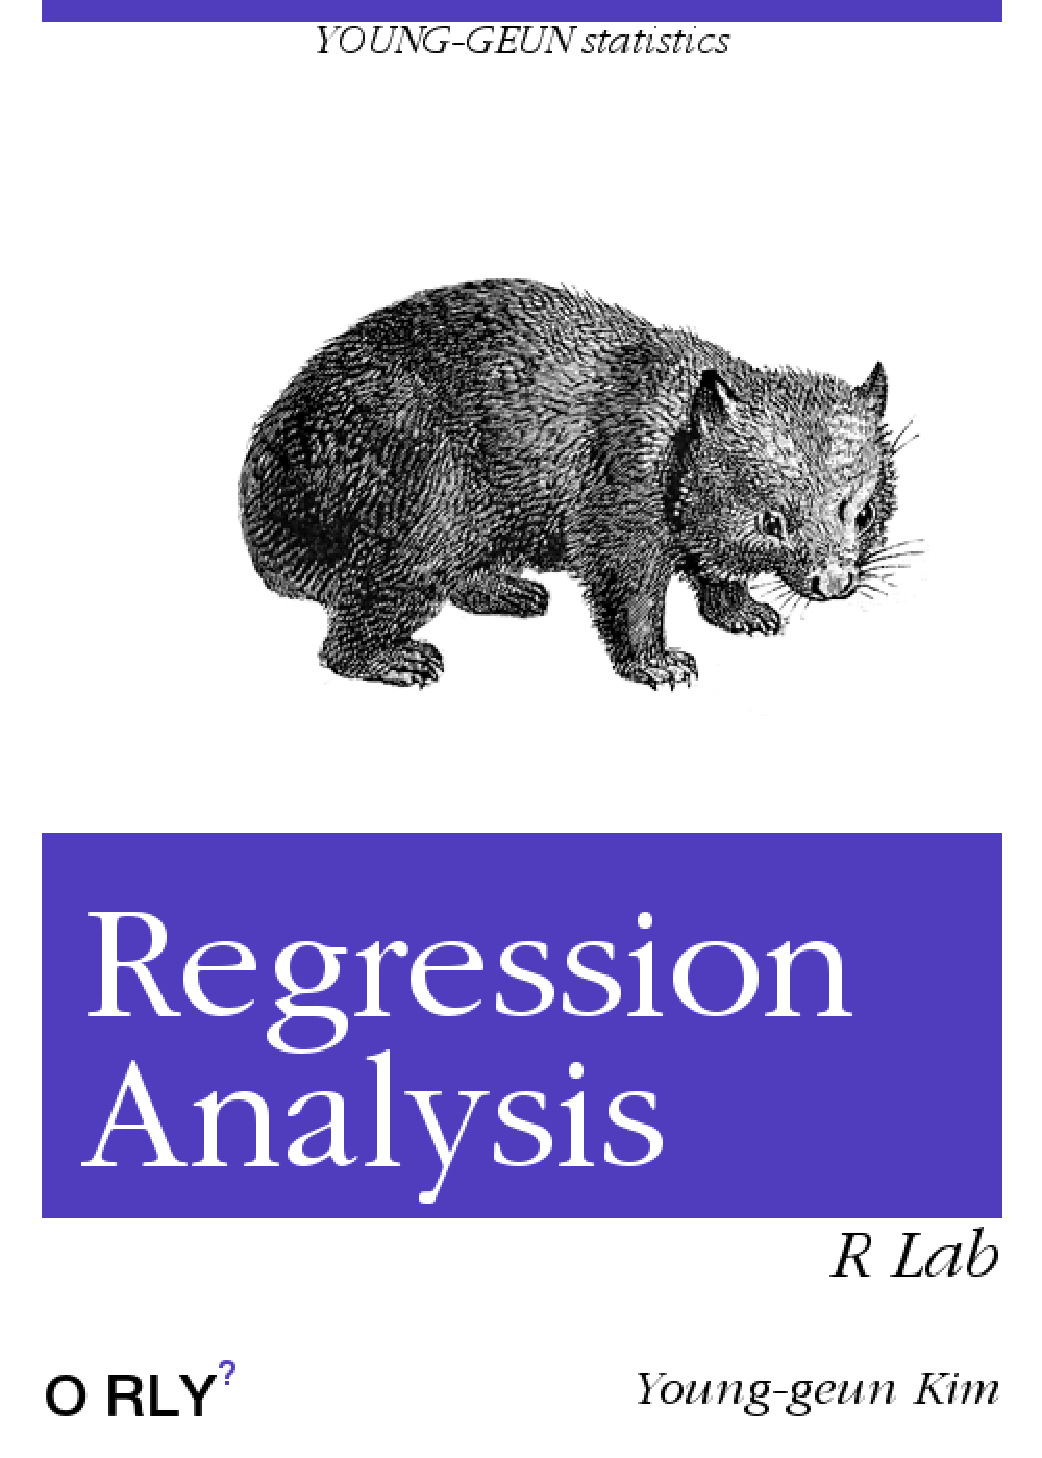
\includepdf{cover.pdf}
\end{titlepage}

\let\maketitle\oldmaketitle
\maketitle

{
\setcounter{tocdepth}{1}
\tableofcontents
}
\hypertarget{welcome}{%
\chapter*{Welcome}\label{welcome}}
\addcontentsline{toc}{chapter}{Welcome}

This book aims at covering materials of regression analysis. Also, there will be R programming for regression.

\begin{Shaded}
\begin{Highlighting}[]
\KeywordTok{library}\NormalTok{(tidyverse)}
\end{Highlighting}
\end{Shaded}

\texttt{tidyverse} package will be used in every chapter, so loading step will be hidden.

\hypertarget{linear-regression-analysis}{%
\section*{Linear Regression Analysis}\label{linear-regression-analysis}}
\addcontentsline{toc}{section}{Linear Regression Analysis}

\begin{Shaded}
\begin{Highlighting}[]
\KeywordTok{data}\NormalTok{(BioOxyDemand, }\DataTypeTok{package =} \StringTok{"MPV"}\NormalTok{)}
\NormalTok{(BioOxyDemand <-}
\StringTok{  }\NormalTok{BioOxyDemand }\OperatorTok\StringTok{ }
\StringTok{  }\KeywordTok{tbl_df}\NormalTok{())}
\CommentTok{#> # A tibble: 14 x 2}
\CommentTok{#>       x     y}
\CommentTok{#>   <int> <int>}
\CommentTok{#> 1     3     4}
\CommentTok{#> 2     8     7}
\CommentTok{#> 3    10     8}
\CommentTok{#> 4    11     8}
\CommentTok{#> 5    13    10}
\CommentTok{#> 6    16    11}
\CommentTok{#> # ... with 8 more rows}
\end{Highlighting}
\end{Shaded}

\hypertarget{relation}{%
\subsection*{Relation}\label{relation}}
\addcontentsline{toc}{subsection}{Relation}

We wonder how \texttt{x} affects \texttt{y}, especially linearly.

\begin{itemize}
\tightlist
\item
  Functional relation: mathematical equation, \[y = \beta_0 + \beta_1 x\]
\item
  Statistical relation: embeded with noise
\end{itemize}

So we try to estimate

\[y = \beta_0 + \beta_1 x + \epsilon\]

\begin{Shaded}
\begin{Highlighting}[]
\NormalTok{BioOxyDemand }\OperatorTok\StringTok{ }
\StringTok{  }\KeywordTok{ggplot}\NormalTok{(}\KeywordTok{aes}\NormalTok{(x, y)) }\OperatorTok{+}
\StringTok{  }\KeywordTok{geom_point}\NormalTok{()}
\end{Highlighting}
\end{Shaded}

\begin{center}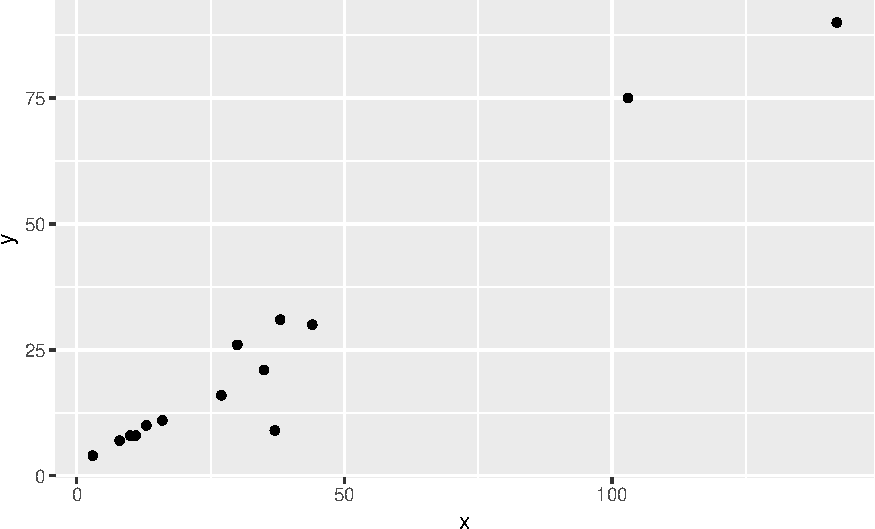
\includegraphics[width=0.7\linewidth]{regression-analysis_files/figure-latex/unnamed-chunk-5-1} \end{center}

Looking just with the eyes, we can see the linear relationship. Regression analysis estimates the relationship statistically.

\begin{Shaded}
\begin{Highlighting}[]
\NormalTok{BioOxyDemand }\OperatorTok\StringTok{ }
\StringTok{  }\KeywordTok{ggplot}\NormalTok{(}\KeywordTok{aes}\NormalTok{(x, y)) }\OperatorTok{+}
\StringTok{  }\KeywordTok{geom_smooth}\NormalTok{(}\DataTypeTok{method =} \StringTok{"lm"}\NormalTok{) }\OperatorTok{+}
\StringTok{  }\KeywordTok{geom_point}\NormalTok{()}
\end{Highlighting}
\end{Shaded}

\begin{center}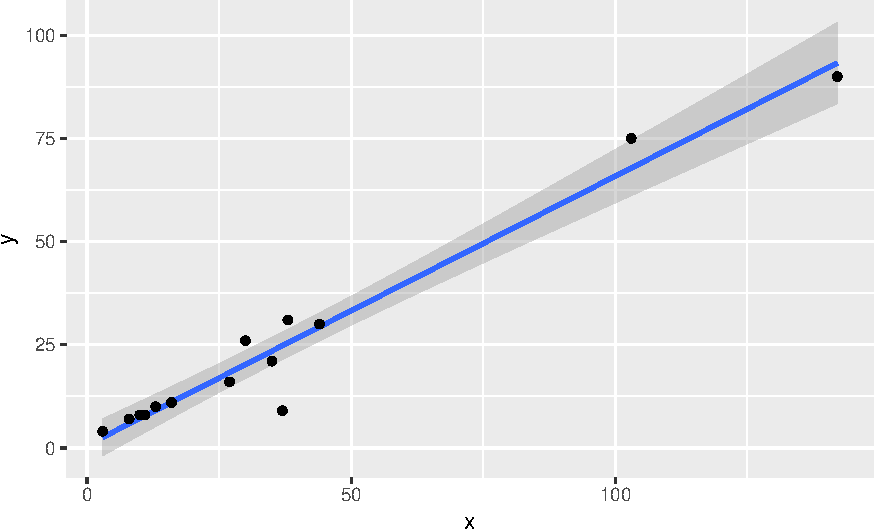
\includegraphics[width=0.7\linewidth]{regression-analysis_files/figure-latex/unnamed-chunk-6-1} \end{center}

\hypertarget{simple}{%
\chapter{Simple Linear Regression}\label{simple}}

\hypertarget{model}{%
\section{Model}\label{model}}

\begin{Shaded}
\begin{Highlighting}[]
\NormalTok{delv <-}\StringTok{ }\NormalTok{MPV}\OperatorTok{::}\NormalTok{p2}\FloatTok{.9} \OperatorTok\StringTok{ }\KeywordTok{tbl_df}\NormalTok{()}
\end{Highlighting}
\end{Shaded}

\begin{Shaded}
\begin{Highlighting}[]
\NormalTok{delv }\OperatorTok\StringTok{ }
\StringTok{  }\KeywordTok{ggplot}\NormalTok{(}\KeywordTok{aes}\NormalTok{(}\DataTypeTok{x =}\NormalTok{ x, }\DataTypeTok{y =}\NormalTok{ y)) }\OperatorTok{+}
\StringTok{  }\KeywordTok{geom_point}\NormalTok{() }\OperatorTok{+}
\StringTok{  }\KeywordTok{labs}\NormalTok{(}
    \DataTypeTok{x =} \StringTok{"Number of Cases"}\NormalTok{,}
    \DataTypeTok{y =} \StringTok{"Delivery Time"}
\NormalTok{  )}
\end{Highlighting}
\end{Shaded}

\begin{figure}[H]

{\centering 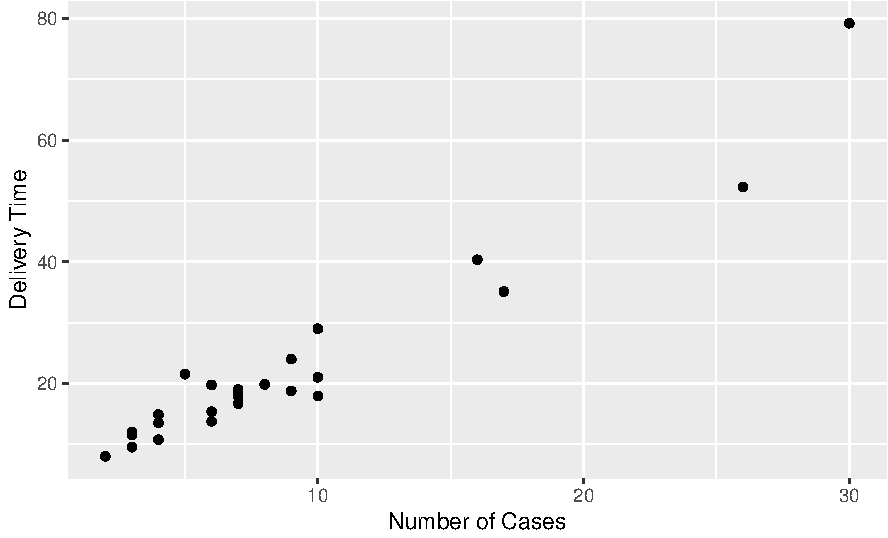
\includegraphics[width=0.7\linewidth]{regression-analysis_files/figure-latex/delivery-1} 

}

\caption{The Delivery Time Data}\label{fig:delivery}
\end{figure}

Given data \((x_1, Y_1), \ldots, (x_n, Y_n)\), we try to fit linear model

\[Y_i = \beta_0 + \beta_1 x_i + \epsilon_i\]

Here \(\epsilon_i\) is a error term, which is a random variable.

\[\epsilon \stackrel{iid}{\sim} (0, \sigma^2)\]

It gives the problem of estimating three parameters \((\beta_0, \beta_1, \sigma^2)\). Before estimating these, we set some assumptions.

\begin{enumerate}
\def\labelenumi{\arabic{enumi}.}
\tightlist
\item
  linear relationship
\item
  \(\epsilon_i\)s are independent
\item
  \(\epsilon_i\)s are identically destributed, i.e.~\emph{constant variance}
\item
  In some setting, \(\epsilon_i \sim N\)
\end{enumerate}

\hypertarget{least-squares-estimation}{%
\section{Least Squares Estimation}\label{least-squares-estimation}}

\begin{figure}[H]

{\centering 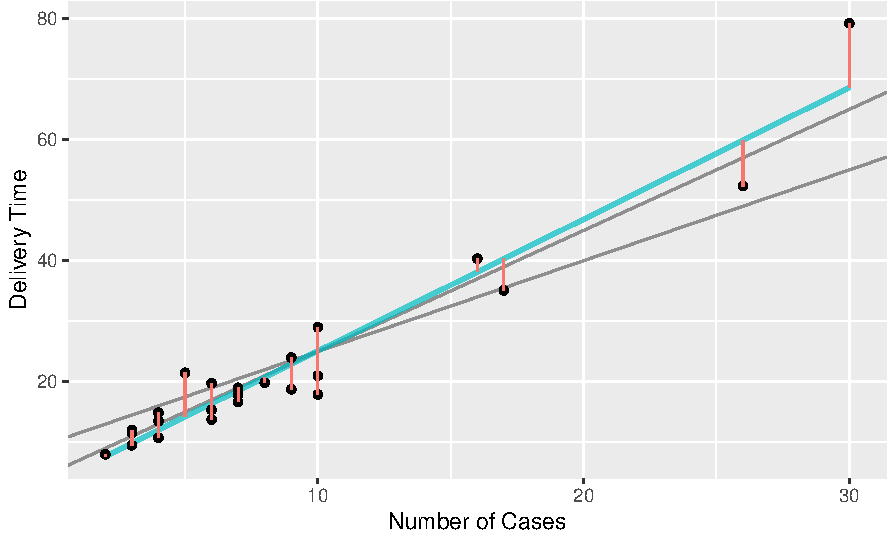
\includegraphics[width=0.7\linewidth]{regression-analysis_files/figure-latex/lsefig-1} 

}

\caption{Idea of the least square estimation}\label{fig:lsefig}
\end{figure}

We try to find \(\beta_0\) and \(\beta_1\) that minimize the sum of squares of the vertical distances, i.e.

\begin{equation}
  (\beta_0, \beta_1) = \arg\min \sum_{i = 1}^n (Y_i - \beta_0 - \beta_1 x_i)^2
  \label{eq:ssq}
\end{equation}

\hypertarget{normal-equations}{%
\subsection{Normal equations}\label{normal-equations}}

Denote that Equation \eqref{eq:ssq} is quadratic. Then we can find its minimum by find the zero point of the first derivative. Set

\[Q(\beta_0, \beta_1) := \sum_{i = 1}^n (Y_i - \beta_0 - \beta_1 x_i)^2\]

Then we have

\begin{equation}
  \frac{\partial Q}{\partial \beta_0} = -2 \sum_{i = 1}^n(Y_i - \beta_0 - \beta_1 x_i) = 0
  \label{eq:normbeta0}
\end{equation}

and

\begin{equation}
  \frac{\partial Q}{\partial \beta_1} = -2 \sum_{i = 1}^n (Y_i - \beta_0 - \beta_1 x_i)x_i = 0
  \label{eq:normbeta1}
\end{equation}

From Equation \eqref{eq:normbeta0},

\[\sum_{i = 1}^n Y_i - n \hat\beta_0 - \hat\beta_1 \sum_{i = 1}^n x_i = 0\]

Thus,

\[\hat\beta_0 = \overline{Y} - \hat\beta_1 \overline{x}\]

Equation \eqref{eq:normbeta1} gives

\[\sum_{i = 1}^n x_i (Y_i - \overline{Y} + \hat\beta_1\overline{x} - \hat\beta_1 x_i) = \sum_{i = 1}^n x_i(Y_i - \overline{Y}) - \hat\beta_1\sum_{i = 1}^n x_i (x_i - \overline{x}) = 0\]

Thus,

\[\hat\beta_1 = \frac{\sum\limits_{i = 1}^nx_i(Y_i - \overline{Y})}{\sum\limits_{i = 1}^n x_i (x_i - \overline{x})}\]

\BeginKnitrBlock{remark}
\iffalse{} {Remark. } \fi{}\[\hat\beta_1 = \frac{S_{XY}}{S_{XX}}\]

where \(S_{XX} := \sum\limits_{i = 1}^n (x_i - \overline{x})^2\) and \(S_{XY} := \sum\limits_{i = 1}^n (x_i - \overline{x})(Y_i - \overline{Y})\)
\EndKnitrBlock{remark}

\BeginKnitrBlock{proof}
\iffalse{} {Proof. } \fi{}Note that \(\overline{x}^2 = \frac{1}{n^2}\bigg(\sum\limits_{i = 1}^n x_i\bigg)^2\). Then we have

\begin{equation}
  \begin{split}
    S_{XX} & = \sum_{i = 1}^n (x_i - \overline{x})^2 \\
    & = \sum_{i = 1}^n x_i^2 - 2\sum_{i = 1}^n x_i \overline{x} + \sum_{i = 1}^n\overline{x}^2 \\
    & = \sum_{i = 1}^n x_i^2 - \frac{2}{n}\bigg(\sum\limits_{i = 1}^n x_i\bigg)^2 + \frac{1}{n}\bigg(\sum\limits_{i = 1}^n x_i\bigg)^2 \\
    & = \sum_{i = 1}^n x_i^2 - \frac{1}{n}\bigg(\sum\limits_{i = 1}^n x_i\bigg)^2
  \end{split}
  \label{eq:sxx}
\end{equation}

It follows that

\begin{equation*}
  \begin{split}
    \hat\beta_1 & = \frac{\sum x_i(Y_i - \overline{Y})}{\sum x_i (x_i - \overline{x})} \\
    & = \frac{\sum x_i (Y_i - \overline{Y}) - \overline{x}\sum (Y_i - \overline{Y})}{\sum x_i^2 - \frac{1}{n} (\sum x_i)^2} \qquad \because \sum (Y_i - \overline{Y}) = 0 \\
    & = \frac{\sum (x_i - \overline{x})(Y_i - \overline{Y})}{\sum x_i^2 - \frac{1}{n} (\sum x_i)^2} \\
    & = \frac{S_{XY}}{S_{XX}}
  \end{split}
\end{equation*}
\EndKnitrBlock{proof}

\begin{Shaded}
\begin{Highlighting}[]
\KeywordTok{lm}\NormalTok{(y }\OperatorTok{~}\StringTok{ }\NormalTok{x, }\DataTypeTok{data =}\NormalTok{ delv)}
\CommentTok{#> }
\CommentTok{#> Call:}
\CommentTok{#> lm(formula = y ~ x, data = delv)}
\CommentTok{#> }
\CommentTok{#> Coefficients:}
\CommentTok{#> (Intercept)            x  }
\CommentTok{#>        3.32         2.18}
\end{Highlighting}
\end{Shaded}

\hypertarget{prediction-and-mean-response}{%
\subsection{Prediction and Mean response}\label{prediction-and-mean-response}}

\begin{quote}
``Essentially, all models are wrong, but some are useful.''

---George Box
\end{quote}

Recall that we have assumed the \textbf{linear assumption} between the predictor and the response variables, i.e.~the true model. Estimating \(\beta_0\) and \(\beta_1\) is same as estimating the \emph{assumed true model}.

\BeginKnitrBlock{definition}[Mean response]
\protect\hypertarget{def:eyx}{}{\label{def:eyx} \iffalse (Mean response) \fi{} }\[E(Y \mid X = x) = \beta_0 + \beta_1 x\]
\EndKnitrBlock{definition}

We can estimate this mean resonse by

\begin{equation}
  \widehat{E(Y \mid x)} = \hat\beta_0 + \hat\beta_1 x
  \label{eq:meanres}
\end{equation}

However, in practice, the model might not be true, which is included in \(\epsilon\) term.

\[Y_i = \beta_0 + \beta_1 x_i + \epsilon_i\]

Our real problem is predicting individual \(Y\), not the mean. The \emph{prediction} of response can be done by

\begin{equation}
  \hat{Y_i}  = \hat\beta_0 + \hat\beta_1 x_i
  \label{eq:indpred}
\end{equation}

Observe that the values of Equations \eqref{eq:meanres} and \eqref{eq:indpred} are same. However, due to the \textbf{error term in the prediction}, it has larger standard error.

\hypertarget{lseprop}{%
\subsection{Properties of LSE}\label{lseprop}}

Parameters \(\beta_0\) and \(\beta_1\) have some properties related to the expectation and variance. We can notice that these lse's are \textbf{unbiased linear estimator}. In fact, these are the \emph{best unbiased linear estimator}. This will be covered in the Gauss-Markov theorem.

\BeginKnitrBlock{lemma}
\protect\hypertarget{lem:sxy}{}{\label{lem:sxy} }\[S_{XX} = \sum_{i = 1}^n x_i^2 - \frac{1}{n}\bigg(\sum\limits_{i = 1}^n x_i\bigg)^2 = \sum_{i = 1}^n x_i(x_i - \overline{x})\]

\[S_{XY} = \sum_{i = 1}^n x_i Y_i - \frac{1}{n}\bigg(\sum_{i = 1}^n x_i\bigg)\bigg(\sum_{i = 1}^n Y_i\bigg) = \sum_{i = 1}^n Y_i(x_i - \overline{x}) = \sum_{i = 1}^n x_i(Y_i - \overline{Y})\]
\EndKnitrBlock{lemma}

\BeginKnitrBlock{proof}
\iffalse{} {Proof. } \fi{}We already proven the first part of \(S_{XX}\). See the Equation \eqref{eq:sxx}. The second part is tivial. Since \(\sum (x_i - \overline{x}) = 0\),

\[S_{XX} = \sum_{i = 1}^n (x_i - \overline{x})^2 = \sum_{i = 1}^n (x_i - \overline{x})x_i\]

For the first part of \(S_{XY}\),

\begin{equation*}
  \begin{split}
    S_{XY} & = \sum_{i = 1}^n (x_i - \overline{x})(Y_i - \overline{Y}) \\
    & = \sum_{i = 1}^n x_i Y_i - \overline{x} \sum_{i = 1}^n Y_i - \overline{Y} \sum_{i = 1}^n x_i + n \overline{x} \overline{Y} \\
    & = \sum_{i = 1}^n x_i Y_i - \frac{1}{n}\bigg(\sum_{i = 1}^n x_i\bigg)\bigg(\sum_{i = 1}^n Y_i\bigg)
  \end{split}
\end{equation*}

Second part of \(S_{XY}\) also can be proven from the definition.

\begin{equation*}
  \begin{split}
    S_{XY} & = \sum_{i = 1}^n (x_i - \overline{x})(Y_i - \overline{Y}) \\
    & = \sum_{i = 1}^n Y_i (x_i - \overline{x}) - \overline{Y} \sum_{i = 1}^n (x_i - \overline{x}) \\
    & = \sum_{i = 1}^n Y_i (x_i - \overline{x}) \qquad \because \sum_{i = 1}^n (x_i - \overline{x}) = 0
  \end{split}
\end{equation*}

Same for the last part.
\EndKnitrBlock{proof}

\BeginKnitrBlock{lemma}[Linearity]
\protect\hypertarget{lem:linbet}{}{\label{lem:linbet} \iffalse (Linearity) \fi{} }Each coefficient is a linear estimator.

\[\hat\beta_1 = \sum_{i = 1}^n\frac{(x_i - \overline{x})}{S_{XX}}Y_i\]

\[\hat\beta_0 = \sum_{i = 1}^n \bigg( \frac{1}{n} - \frac{(x_i - \overline{x})\overline{x}}{S_{XX}} \bigg) Y_i\]
\EndKnitrBlock{lemma}

\BeginKnitrBlock{proof}
\iffalse{} {Proof. } \fi{}From lemma \ref{lem:sxy},

\begin{equation*}
  \begin{split}
    \hat\beta_1 & = \frac{S_{XY}}{S_{XX}} \\
    & = \frac{1}{S_{XX}}\sum_{i = 1}^n (x_i - \overline{x}) Y_i
  \end{split}
\end{equation*}

It gives that

\begin{equation*}
  \begin{split}
    \hat\beta_0 & = \overline{Y} - \hat\beta_1 \overline{x} \\
    & = \frac{1}{n}\sum_{i = 1}^n Y_i - \overline{x} \sum_{i = 1}^n\frac{(x_i - \overline{x})}{S_{XX}}Y_i \\
    & = \sum_{i = 1}^n\bigg(\frac{1}{n} - \frac{(x_i - \overline{x})\overline{x}}{S_{XX}} \bigg)Y_i
  \end{split}
\end{equation*}
\EndKnitrBlock{proof}

\BeginKnitrBlock{proposition}[Unbiasedness]
\protect\hypertarget{prp:ue}{}{\label{prp:ue} \iffalse (Unbiasedness) \fi{} }Both coefficients are unbiased.

\begin{enumerate}
  \item $E\hat\beta_1 = \beta_1$
  \item $E\hat\beta_0 = \beta_0$
\end{enumerate}
\EndKnitrBlock{proposition}

From the model, \(Y_1, \ldots, Y_n \stackrel{indep}{\sim} (\beta_0 + \beta_1 x_i, \sigma^2)\).

\BeginKnitrBlock{proof}
\iffalse{} {Proof. } \fi{}From lemma \ref{lem:sxy},

\begin{equation*}
  \begin{split}
    E\hat\beta_1 & = \sum_{i = 1}^n \bigg[ \frac{(x_i - \overline{x})}{S_{XX}} E(Y_i) \bigg] \\
    & = \sum_{i = 1}^n \frac{(x_i - \overline{x})}{S_{XX}}(\beta_0 + \beta_1 x_i) \\
    & = \frac{\beta_1 \sum (x_i - \overline{x})x_i}{\sum (x_i - \overline{x})x_i} \qquad \because \sum (x_i - \overline{x}) = 0 \\
    & = \beta_1
  \end{split}
\end{equation*}

It follows that

\begin{equation*}
  \begin{split}
    E\hat\beta_0 & = E(\overline{Y} - \hat\beta_1 \overline{x}) \\
    & = E(\overline{Y}) - \overline{x}E(\hat\beta_1) \\
    & = E(\beta_0 + \beta_1 \overline{x} + \overline{\epsilon}) - \beta_1 \overline{x} \\
    & = \beta_0 + \beta_1 \overline{x} - \beta_1 \overline{x} \\
    & = \beta_0
  \end{split}
\end{equation*}
\EndKnitrBlock{proof}

\BeginKnitrBlock{proposition}[Variances]
\protect\hypertarget{prp:vb}{}{\label{prp:vb} \iffalse (Variances) \fi{} }Variances and covariance of coefficients

\begin{enumerate}[label=(\alph*)]
  \item $Var\hat\beta_1 = \frac{\sigma^2}{S_{XX}}$ \label{itm:vbone}
  \item $Var\hat\beta_0 = \bigg( \frac{1}{n} + \frac{\overline{x}^2}{S_{XX}} \bigg)\sigma^2$ \label{itm:vbtwo}
  \item $Cov(\hat\beta_0, \hat\beta_1) = - \frac{\overline{x}}{S_{XX}} \sigma^2$ \label{itm:vbthree}
\end{enumerate}
\EndKnitrBlock{proposition}

\BeginKnitrBlock{proof}
\iffalse{} {Proof. } \fi{}Proving is just arithmetic.

\(\ref{itm:vbone}\)

\begin{equation*}
  \begin{split}
    Var\hat\beta_1 & = \frac{1}{S_{XX}^2}\sum_{i = 1}^n \bigg[ (x_i - \overline{x})^2 Var(Y_i) \bigg] + \frac{1}{S_{XX}^2} \sum_{j \neq k}^n \bigg[ (x_j - \overline{x})(x_k - \overline{x}) Cov(Y_j, Y_k) \bigg] \\
    & = \frac{\sigma^2}{S_{XX}} \qquad \because Cov(Y_j, Y_k) = 0 \: \text{if} \: j \neq k
  \end{split}
\end{equation*}

\(\ref{itm:vbtwo}\)

\begin{equation*}
  \begin{split}
    Var\hat\beta_0 & = \sum_{i = 1}^n \bigg( \frac{1}{n} - \frac{(x_i - \overline{x})\overline{x}}{S_{XX}} \bigg)^2Var(Y_i) + \sum_{j \neq k} \bigg( \frac{1}{n} - \frac{(x_j - \overline{x})\overline{x}}{S_{XX}} \bigg)\bigg( \frac{1}{n} - \frac{(x_k - \overline{x})\overline{x}}{S_{XX}} \bigg) Cov(Y_j, Y_k) \\
    & = \frac{\sigma^2}{n} - 2 \sigma^2 \frac{\overline{x}}{S_{XX}} \sum_{i = 1}^n (x_i - \overline{x}) + \frac{\sigma^2 \overline{x}^2 \sum (x_i - \overline{x})^2}{S_{XX}^2} \\
    & = \bigg( \frac{1}{n} + \frac{\overline{x}^2}{S_{XX}} \bigg) \sigma^2 \qquad \because \sum (x_i - \overline{x}) = 0
  \end{split}
\end{equation*}

\(\ref{itm:vbthree}\)

\begin{equation*}
  \begin{split}
    Cov(\hat\beta_0, \hat\beta_1) & = Cov(\overline{Y} - \hat\beta_1 \overline{x}, \hat\beta_1) \\
    & = - \overline{x} Var\hat\beta_1 \\
    & = - \frac{\overline{x}}{S_{XX}} \sigma^2
  \end{split}
\end{equation*}
\EndKnitrBlock{proof}

\hypertarget{gauss-markov-theorem}{%
\subsection{Gauss-Markov Theorem}\label{gauss-markov-theorem}}

Chapter \ref{lseprop} shows that the \(\beta_0^{LSE}\) and \(\beta_1^{LSE}\) are the \textbf{linear unbiased estimators}. Are these good? Good compared to \emph{what estimators}? Here we consider \emph{linear unbiased estimator}. If variances in the proposition \ref{prp:vb} are lower than any parameters in this parameter family, \(\beta_0^{LSE}\) and \(\beta_1^{LSE}\) are the \textbf{best linear unbiased estimators}.

\BeginKnitrBlock{theorem}[Gauss Markov Theorem]
\protect\hypertarget{thm:gmt}{}{\label{thm:gmt} \iffalse (Gauss Markov Theorem) \fi{} }\(\hat\beta_0\) and \(\hat\beta_1\) are BLUE, i.e.~the best linear unbiased estimator.

\[Var(\hat\beta_0) \le Var\Big( \sum_{i = 1}^n a_i Y_i \Big) \: \forall a_i \in \mathbb{R} \: \text{s.t.} \: E\Big( \sum_{i = 1}^n a_i Y_i \Big) = \beta_0\]

\[Var(\hat\beta_1) \le Var\Big( \sum_{i = 1}^n b_i Y_i \Big) \: \forall b_i \in \mathbb{R} \: \text{s.t.} \: E\Big( \sum_{i = 1}^n b_i Y_i \Big) = \beta_1\]
\EndKnitrBlock{theorem}

\BeginKnitrBlock{proof}[Bestness of $\beta_1$]
\iffalse{} {Proof (Bestness of \(\beta_1\)). } \fi{}Consider \(\Theta := \bigg\{ \sum\limits_{i = 1}^n b_i Y_i \in \mathbb{R} : E\Big( \sum\limits_{i = 1}^n b_i Y_i \Big) = \beta_1 \bigg\}\).

Claim: \(Var( \sum b_i Y_i) - Var(\hat\beta_1) \ge 0\)

Let \(\sum b_i Y_i \in \Theta\). Then \(E(\sum b_i Y_i) = \beta_1\).

Since \(E(Y_i) = \beta_0 + \beta_1 x_i\),

\[\beta_0 \sum b_i + \beta_1 \sum b_i x_i = \beta_1\]

It gives

\begin{equation} \label{eq:ule}
  \begin{cases}
    \sum b_i = 0 \\
    \sum b_i x_i = 1
  \end{cases}
\end{equation}

Then

\begin{equation*}
  \begin{split}
    0 \le Var\Big(\sum b_i Y_i - \hat\beta_1\Big) & = Var\Big( \sum b_i Y_i - \sum \frac{(x_i - \bar{x})}{S_{XX}} Y_i \Big) \\
    & \stackrel{indep}{=} \sum \bigg( b_i - \frac{(x_i - \bar{x})}{S_{XX}} \bigg)^2 \sigma^2 \\
    & = \sum \bigg( b_i^2 - \frac{2b_i (x_i - \bar{x})}{S_{XX}} + \frac{(x_i - \bar{x})^2}{S_{XX}^2} \bigg) \sigma^2 \\
    & = \sum b_i^2 \sigma^2 - \frac{2 \sigma^2}{S_{XX}} \sum b_i x_i + \frac{2 \bar{x} \sigma^2}{S_{XX}} \sum b_i + \sigma^2 \frac{\sum (x_i - \bar{x})^2}{S_{XX}^2} \\
    & = \sum b_i^2 \sigma^2 - \frac{\sigma^2}{S_{XX}} \qquad \because \eqref{eq:ule} \:\text{and}\: S_{XX} = \sum (x_i - \bar{x})^2 \\
    & = Var(\sum b_i Y_i) - Var(\hat\beta_1)
  \end{split}
\end{equation*}

Hence,

\[Var(\sum b_i Y_i) \ge Var(\hat\beta_1)\]
\EndKnitrBlock{proof}

\BeginKnitrBlock{proof}[Bestness of $\beta_0$]
\iffalse{} {Proof (Bestness of \(\beta_0\)). } \fi{}Consider \(\Theta := \bigg\{ \sum\limits_{i = 1}^n a_i Y_i \in \mathbb{R} : E\Big( \sum\limits_{i = 1}^n a_i Y_i \Big) = \beta_0 \bigg\}\).

Claim: \(Var( \sum a_i Y_i) - Var(\hat\beta_0) \ge 0\)

Let \(\sum a_i Y_i \in \Theta\). Then \(E(\sum a_i Y_i) = \beta_0\).

Since \(E(Y_i) = \beta_0 + \beta_1 x_i\),

\[\beta_0 \sum a_i + \beta_1 \sum a_i x_i = \beta_0\]

It gives

\begin{equation} \label{eq:ule0}
  \begin{cases}
    \sum a_i = 1 \\
    \sum a_i x_i = 0
  \end{cases}
\end{equation}

Then

\begin{equation*}
  \begin{split}
    0 \le Var\Big(\sum a_iY_i - \hat\beta_0 \Big) & = Var\bigg[\sum a_iY_i - \sum\Big( \frac{1}{n} - \frac{(x_k - \bar{x})\bar{x}}{S_{XX}} \Big) Y_k \bigg] \\
    & = \sum \bigg(a_i - \frac{1}{n} +  \frac{(x_i - \bar{x})\bar{x}}{S_{XX}} \bigg)^2\sigma^2 \\
    & = \sum \bigg[ a_i^2 - 2a_i\Big( \frac{1}{n} - \frac{(x_i - \bar{x})\bar{x}}{S_{XX}} \Big) + \Big( \frac{1}{n} - \frac{(x_i - \bar{x})\bar{x}}{S_{XX}} \Big)^2 \bigg]\sigma^2 \\
        & = \sum a_i^2\sigma^2 -\frac{2\sigma^2}{n}\sum a_i + \frac{2\bar{x}\sigma^2\sum a_ix_i}{S_{XX}} - \frac{2\bar{x}^2\sigma^2\sum a_i}{S_{XX}} \\
        & \qquad + \sigma^2\bigg( \frac{1}{n} - \frac{2\bar{x}}{nS_{XX}} \sum(x_i - \bar{x}) + \frac{\bar{x}^2\sum(x_i - \bar{x})^2}{S_{XX}^2} \bigg) \\
        & = \sum a_i^2\sigma^2 -\frac{2\sigma^2}{n} - \frac{2\bar{x}^2\sigma^2}{S_{XX}} \qquad \because \eqref{eq:ule0} \\
        & \qquad + \bigg(\frac{1}{n} + \frac{\bar{x}^2}{S_{XX}} \bigg)\sigma^2 \qquad \because \sum(x_i - \bar{x}) = 0 \: \text{and} \: S_{XX} := \sum (x_i - \bar{x})^2 \\
        & = \sum a_i^2\sigma^2 - \bigg( \frac{1}{n} + \frac{\bar{x}^2}{S_{XX}} \bigg)\sigma^2 \\
        & = Var\Big( \sum a_i Y_i \Big) - Var\hat\beta_0
  \end{split}
\end{equation*}

Hence,

\[Var(\sum a_i Y_i) \ge Var(\hat\beta_0)\]
\EndKnitrBlock{proof}

\BeginKnitrBlock{example}
\protect\hypertarget{exm:usingnormal}{}{\label{exm:usingnormal} }Show that \(\sum (Y_i - \hat{Y_i}) = 0\), \(\sum x_i (Y_i - \hat{Y_i}) = 0\), and \(\sum \hat{Y_i} (Y_i - \hat{Y_i}) = 0\).
\EndKnitrBlock{example}

\BeginKnitrBlock{solution}
\iffalse{} {Solution. } \fi{}Consider the two normal equations \eqref{eq:normbeta0} and \eqref{eq:normbeta1}. Note that \(\hat{Y_i} = \hat\beta_0 + \hat\beta_1 x_i\).

From the Equation \eqref{eq:normbeta0}, we have \(\sum (Y_i - \hat{Y_i}) = 0\).

From the Equation \eqref{eq:normbeta1}, we have \(\sum x_i (Y_i - \hat{Y_i}) = 0\).

It follows that

\begin{equation*}
  \begin{split}
    \sum \hat{Y_i} (Y_i - \hat{Y_i}) & = \sum (\hat\beta_0 + \hat\beta_1 x_i) (Y_i - \hat{Y_i}) \\
    & = \hat\beta_0 \sum (Y_i - \hat{Y_i}) + \hat\beta_1 \sum x_i (Y_i - \hat{Y_i}) \\
    & = 0
  \end{split}
\end{equation*}
\EndKnitrBlock{solution}

\hypertarget{estimation-of-sigma2}{%
\subsection{\texorpdfstring{Estimation of \(\sigma^2\)}{Estimation of \textbackslash sigma\^{}2}}\label{estimation-of-sigma2}}

There is the last parameter, \(\sigma^2 = Var(Y_i)\). In the \emph{least squares estimation literary}, we estimate \(\sigma^2\) by

\begin{equation}
  \hat\sigma^2 = \frac{1}{n - 2} \sum_{i = 1}^n (Y_i - \hat\beta_0 - \hat\beta_1 x_i)^2
  \label{eq:siglse}
\end{equation}

Why \(n - 2\)? This makes the estimator unbiased.

\BeginKnitrBlock{proposition}[Unbiasedness]
\protect\hypertarget{prp:sigex}{}{\label{prp:sigex} \iffalse (Unbiasedness) \fi{} }\[E(\hat\sigma^2) = \sigma^2\]
\EndKnitrBlock{proposition}

\BeginKnitrBlock{proof}
\iffalse{} {Proof. } \fi{}Note that

\[(Y_i - \hat\beta_0 - \hat\beta_1 x_i) = (Y_i - \overline{Y}) - \hat\beta_1(x_i - \overline{x})\]

Then

\begin{equation*}
  \begin{split}
    E(\hat\sigma^2) & = \frac{1}{n - 2} E \bigg[ \sum (Y_i - \hat\beta_0 - \hat\beta_1 x_i)^2 \bigg] \\
    & = \frac{1}{n - 2} E \bigg[ \sum (Y_i - \overline{Y})^2 + \hat\beta_1^2 \sum (x_i - \overline{x})^2 -2\hat\beta_1 \sum (Y_i - \overline{Y})(x_i - \overline{x}) \bigg] \\
    & = \frac{1}{n - 2} E ( S_{YY} + \hat\beta_1^2 S_{XX} - 2 \hat\beta_1 S_{XY}) \\
    & = \frac{1}{n - 2} E ( S_{YY} - \hat\beta_1^2 S_{XX}) \qquad \because S_{XY} = \hat\beta_1 S_{XX} \\
    & = \frac{1}{n - 2} \Big(  \underset{(a)}{\underline{ES_{YY}}} - S_{XX} \underset{(b)}{\underline{E\hat\beta_1^2}} \Big)
  \end{split}
\end{equation*}

\begin{enumerate}
\def\labelenumi{(\alph{enumi})}
\item
\end{enumerate}

\begin{equation*}
  \begin{split}
    ES_{YY} & = E\Big[ \sum (Y_i - \overline{Y})^2 \Big] \\
    & = E \Big[ \sum \Big( (\beta_0 + \beta_1 x_i + \epsilon_i) - (\beta_0 + \beta_1 \overline{x} + \overline{\epsilon}) \Big)^2 \Big] \\
    & = E \Big[ \sum \Big( \beta_1 (x_i - \overline{x}) + (\epsilon_i - \overline{\epsilon}) \Big)^2 \Big] \\
    & = \beta_1^2 S_{XX} + E\Big( \sum (\epsilon_i - \overline{\epsilon})^2 \Big) + 2\beta_1 \sum (x_i - \overline{x}) E(\epsilon_i - \overline{\epsilon}) \\
    & = \beta_1^2 S_{XX} + E\Big( \sum (\epsilon_i - \overline{\epsilon})^2 \Big)
  \end{split}
\end{equation*}

Since \(E(\bar\epsilon) = 0\) and \(Var(\bar\epsilon) = \frac{\sigma^2}{n}\),

\begin{equation*}
  \begin{split}
    E\Big( \sum (\epsilon_i - \overline{\epsilon})^2 \Big) & = E \Big( \sum (\epsilon_i^2 + \bar\epsilon^2 - 2\epsilon_i \bar\epsilon) \Big) \\
    & = \sum E(\epsilon_i^2) - n E(\bar\epsilon^2) \qquad \because \sum \epsilon = n \bar\epsilon \\
    & = \sum (Var(\epsilon_i) + E(\epsilon_i)^2) - n(Var(\bar\epsilon) + E(\bar\epsilon)^2) \\
    & = n\sigma^2 - \sigma^2 \\
    & = (n - 1)\sigma^2
  \end{split}
\end{equation*}

Thus,

\[ES_{YY} = \beta_1^2 S_{XX} + (n - 1)\sigma^2\]

\begin{enumerate}
\def\labelenumi{(\alph{enumi})}
\setcounter{enumi}{1}
\item
\end{enumerate}

\begin{equation*}
  \begin{split}
    E\hat\beta_1^2 & = Var\hat\beta_1 + E(\hat\beta_1)^2 \\
    & = \frac{\sigma^2}{S_{XX}} + \beta_1^2
  \end{split}
\end{equation*}

It follows that

\begin{equation*}
  \begin{split}
    E(\hat\sigma^2) & = \frac{1}{n - 2} \Big(  \underset{(a)}{\underline{ES_{YY}}} - S_{YY} \underset{(b)}{\underline{E\hat\beta_1^2}} \Big) \\
    & = \frac{1}{n - 2} \bigg( \Big(\beta_1^2 S_{XX} + (n - 1)\sigma^2 \Big) - S_{XX}\Big(\frac{\sigma^2}{S_{XX}} + \beta_1^2 \Big) \bigg) \\
    & = \frac{1}{n - 2}((n - 2)\sigma^2) \\
    & = \sigma^2
  \end{split}
\end{equation*}
\EndKnitrBlock{proof}

\hypertarget{maximum-likelihood-estimation}{%
\section{Maximum Likelihood Estimation}\label{maximum-likelihood-estimation}}

In this section, we add an assumption to an random errors \(\epsilon_i\).

\[\epsilon_i \stackrel{iid}{\sim} N(0, \sigma^2)\]

\BeginKnitrBlock{example}[Gaussian Likelihood]
\protect\hypertarget{exm:gmle}{}{\label{exm:gmle} \iffalse (Gaussian Likelihood) \fi{} }Note that \(Y_i \stackrel{indep}{\sim} N(\beta_0 + \beta_1 x_i, \sigma^2)\). Then the likelihood function is

\[L(\beta_0, \beta_1, \sigma^2) = \prod_{i = 1}^n\bigg( \frac{1}{\sqrt{2\pi\sigma^2}} \exp \bigg(- \frac{(Y_i - \beta_0 - \beta_1 x_i)^2}{2 \sigma^2} \bigg) \bigg)\]

and so the log-likelihood function can be computed as

\[l(\beta_0, \beta_1, \sigma^2) = -\frac{n}{2}\ln(2\pi\sigma^2) - \frac{1}{2\sigma^2}\sum_{i = 1}^n(Y_i - \beta_0 - \beta_1 x_i)^2\]
\EndKnitrBlock{example}

\hypertarget{likelihood-equations}{%
\subsection{Likelihood equations}\label{likelihood-equations}}

\BeginKnitrBlock{definition}[Maximum Likelihood Estimator]
\protect\hypertarget{def:mledef}{}{\label{def:mledef} \iffalse (Maximum Likelihood Estimator) \fi{} }\[(\hat\beta_0^{MLE}, \hat\beta_1^{MLE}, \hat\sigma^{2MLE}) := \arg\sup L(\beta_0, \beta_1, \sigma^2)\]
\EndKnitrBlock{definition}

Since \(l(\cdot) = \ln L(\cdot)\) is monotone,

\BeginKnitrBlock{remark}
\iffalse{} {Remark. } \fi{}\[(\hat\beta_0^{MLE}, \hat\beta_1^{MLE}, \hat\sigma^{2MLE}) = \arg\sup l(\beta_0, \beta_1, \sigma^2)\]
\EndKnitrBlock{remark}

We can find the maximum of this \emph{quadratic} function by making first derivative.

\begin{equation}
  \frac{\partial l}{\partial \beta_0} = \frac{1}{\sigma^2} \sum_{i = 1}^n (Y_i - \beta_0 - \beta_1 x_i) = 0
  \label{eq:mlbeta0}
\end{equation}

\begin{equation}
  \frac{\partial l}{\partial \beta_1} = \frac{1}{\sigma^2} \sum_{i = 1}^n x_i (Y_i - \beta_0 - \beta_1 x_i) = 0
  \label{eq:mlbeta1}
\end{equation}

\begin{equation}
  \frac{\partial l}{\partial \sigma^2} = - \frac{n}{2\sigma^2} + \frac{1}{2\sigma^4} \sum_{i = 1}^n (Y_i - \beta_0 - \beta_1 x_i)^2 = 0
  \label{eq:mlsig}
\end{equation}

Denote that Equations \eqref{eq:mlbeta0} and \eqref{eq:mlbeta1} given \(\hat\sigma^2\) are equivalent to the normal equations. Thus,

\[\hat\beta_0^{MLE} = \hat\beta_0^{LSE}, \quad \hat\beta_1^{MLE} = \hat\beta_1^{LSE}\]

From Equation \eqref{eq:mlsig},

\[\hat\sigma^{2MLE} = \frac{1}{n}\sum_{i = 1}^n(Y_i - \beta_0 - \beta_1 x_i)^2 = \frac{n - 2}{n} \hat\sigma^{2LSE}\]

While \(\hat\sigma^{2LSE}\) is an unbiased, above \emph{MLE is not an unbiased estimator}. Since \(\hat\sigma^{2MLE} \approx \hat\sigma^{2LSE}\) for large \(n\), howerver, it is \emph{asymptotically unbiased}.

\BeginKnitrBlock{theorem}[Rao-Cramer Lower Bound, univariate case]
\protect\hypertarget{thm:rclb}{}{\label{thm:rclb} \iffalse (Rao-Cramer Lower Bound, univariate case) \fi{} }Let \(X_1, \ldots, X_n \stackrel{iid}{\sim} f(x ; \theta)\). If \(\hat\theta\) is an unbiased estimator of \(\theta\),

\[Var(\hat\theta) \ge \frac{1}{I_n(\theta)}\]

where \(I_n(\theta) = -E\bigg(\frac{\partial^2 l(\theta)}{\partial \theta^2} \bigg)\)
\EndKnitrBlock{theorem}

To apply this theorem \ref{thm:rclb} in the simple linear regression setting, i.e.~\((\beta_0, \beta_1)\), we need to look at the \emph{bivariate case}.

\BeginKnitrBlock{theorem}[Rao-Cramer Lower Bound, bivariate case]
\protect\hypertarget{thm:rclb2}{}{\label{thm:rclb2} \iffalse (Rao-Cramer Lower Bound, bivariate case) \fi{} }Let \(X_1, \ldots, X_n \stackrel{iid}{\sim} f(x ; \theta1, \theta_2)\) and let \(\boldsymbol{\theta} = (\theta_1, \theta_2)^T\). If each \(\hat\theta_1\), \(\hat\theta_2\) is an unbiased estimator of \(\theta_1\) and \(\theta_2\), then

\[
Var(\boldsymbol{\theta}) := \begin{bmatrix}
Var(\hat\theta_1) & Cov(\hat\theta_1, \hat\theta_2) \\
Cov(\hat\theta_1, \hat\theta_2) & Var(\hat\theta_2)
\end{bmatrix} \ge I_n^{-1}(\theta_1, \theta_2)
\]

where

\[
I_n(\theta_1, \theta_2) = - \begin{bmatrix}
  E\bigg( \frac{\partial^2 l(\theta_1, \theta_2)}{\partial \theta_1^2} \bigg) & E\bigg( \frac{\partial^2 l(\theta_1, \theta_2)}{\partial \theta_1 \partial \theta_2} \bigg) \\
  E\bigg( \frac{\partial^2 l(\theta_1, \theta_2)}{\partial \theta_1 \partial \theta_2} \bigg) & E\bigg( \frac{\partial^2 l(\theta_1, \theta_2)}{\partial \theta_2^2} \bigg)
\end{bmatrix}
\]
\EndKnitrBlock{theorem}

Assume that \(\sigma^2\) is \textbf{known}. From the Equations \eqref{eq:mlbeta0} and \eqref{eq:mlbeta1},

\[
\begin{cases}
  \frac{\partial^2 l}{\partial \beta_0^2} = - \frac{n}{\sigma^2} \\
  \frac{\partial^2 l}{\partial \beta_1^2} = - \frac{\sum x_i^2}{\sigma^2} \\
  \frac{\partial^2 l}{\partial \beta_0 \partial \beta_1} = - \frac{\sum x_i}{\sigma^2}
\end{cases}
\]

Thus,

\[
I_n(\beta_0, \beta_1) = \begin{bmatrix}
  \frac{n}{\sigma^2} & \frac{\sum x_i}{\sigma^2} \\
  \frac{\sum x_i}{\sigma^2} & \frac{\sum x_i^2}{\sigma^2}
\end{bmatrix}
\]

Applying gaussian elimination,

\begin{equation*}
  \begin{split}
    \left[
    \begin{array}{cc|cc}
      \frac{n}{\sigma^2} & \frac{\sum x_i}{\sigma^2} & 1 & 0 \\
      \frac{\sum x_i}{\sigma^2} & \frac{\sum x_i^2}{\sigma^2} & 0 & 1
    \end{array}
    \right] & \leftrightarrow \left[
    \begin{array}{cc|cc}
      \frac{n}{\sigma^2} & \frac{\sum x_i}{\sigma^2} & 1 & 0 \\
      \frac{\sum x_i}{\sigma^2}\Big(\frac{n}{\sum x_i} \Big) & \frac{\sum x_i^2}{\sigma^2}\Big(\frac{n}{\sum x_i} \Big) & 0 & \frac{1}{\overline{x}}
    \end{array}
    \right] \\
    & \leftrightarrow \left[
    \begin{array}{cc|cc}
      \frac{n}{\sigma^2} & \frac{\sum x_i}{\sigma^2} & 1 & 0 \\
      0 & \frac{\sum x_i^2 - \overline{x}\sum x_i}{\sigma^2\overline{x}} = \frac{S_{XX}}{\sigma^2\overline{x}} & -1 & \frac{1}{\overline{x}}
    \end{array}
    \right] \\
    & \leftrightarrow \left[
    \begin{array}{cc|cc}
      1 & \overline{x} & \frac{\sigma^2}{n} & 0 \\
      0 & 1 & -\frac{\overline{x}}{S_{XX}}\sigma^2 & \frac{\sigma^2}{S_{XX}}
    \end{array}
    \right] \\
    & \leftrightarrow \left[
    \begin{array}{cc|cc}
      1 & 0 & \bigg(\frac{1}{n} + \frac{\overline{x}^2}{S_{XX}} \bigg)\sigma^2 & -\frac{\overline{x}}{S_{XX}}\sigma^2 \\
      0 & 1 & -\frac{\overline{x}}{S_{XX}}\sigma^2 & \frac{\sigma^2}{S_{XX}}
    \end{array}
    \right]
  \end{split}
\end{equation*}

Hence,

\[
I_n^{-1}(\beta_0, \beta_1) = \begin{bmatrix}
  \bigg(\frac{1}{n} + \frac{\overline{x}^2}{S_{XX}} \bigg)\sigma^2 & -\frac{\overline{x}}{S_{XX}}\sigma^2 \\
  -\frac{\overline{x}}{S_{XX}}\sigma^2 & \frac{\sigma^2}{S_{XX}}
\end{bmatrix} = \begin{bmatrix}
  Var(\hat\beta_0) & Cov(\hat\beta_0, \hat\beta_1) \\
  Cov(\hat\beta_0, \hat\beta_1) & Var(\hat\beta_1)
\end{bmatrix}
\]

Since \(Var(\boldsymbol{\hat\beta}) - I^{-1} = 0\) is non-negative definite, each \(Var(\hat\beta_0) = \bigg(\frac{1}{n} + \frac{\overline{x}^2}{S_{XX}} \bigg)\sigma^2\) and \(Var(\hat\beta_1) = \frac{\sigma^2}{S_{XX}}\) is a theoretical bound.

\BeginKnitrBlock{remark}
\iffalse{} {Remark. } \fi{}This says that \(\hat\beta_0^{LSE} = \hat\beta_0^{MLE}\) and \(\hat\beta_1^{LSE} = \hat\beta_1^{MLE}\) have the smallest variance among all unbiased estimator.
\EndKnitrBlock{remark}

This result is \emph{stronger than Gauss-Markov theorem} \ref{thm:gmt}, where the LSE has the smalleset variance among all \emph{linear unbiased} estimators. It can be simply obtained from the \emph{Lehmann-Scheffe Theorem}: If some unbiased estimator is a function of complete sufficient statistic, then this estimator is the unique MVUE \citep{Hogg:2018aa}.

\BeginKnitrBlock{remark}[Lehmann and Scheffe for regression coefficients]
\iffalse{} {Remark (Lehmann and Scheffe for regression coefficients). } \fi{}\(u\Big(\sum Y_i, S_{XY} \Big)\) is CSS in this regression problem, i.e.~known \(\sigma^2\).
\EndKnitrBlock{remark}

\BeginKnitrBlock{proof}
\iffalse{} {Proof. } \fi{}From the example \ref{exm:gmle},

\begin{equation*}
  \begin{split}
    L(\beta_0, \beta_1) & = (2\pi\sigma^2)^{-\frac{n}{2}}\exp\bigg[-\frac{1}{2\sigma^2} \sum(Y_i - \beta_0 - \beta_1 x_i)^2 \bigg] \\
    & = (2\pi\sigma^2)^{-\frac{n}{2}}\exp\bigg[-\frac{1}{2\sigma^2} \sum \Big(Y_i^2 - (\beta_0 + \beta_1 x_i)Y_i + (\beta_0 + \beta_1 x_i)^2 \Big) \bigg] \\
    & = (2\pi\sigma^2)^{-\frac{n}{2}}\exp\bigg[-\frac{1}{2\sigma^2} \Big( -\beta_0 \sum Y_i - \beta_1 \sum x_i Y_i \Big) \bigg] \exp\bigg[-\frac{1}{2\sigma^2} \Big( \sum Y_i^2 + (\beta_0 + \beta_1 x_i)^2 \Big) \bigg]
  \end{split}
\end{equation*}

By the Factorization theorem, both \(\sum Y_i\) and \(\sum x_i Y_i\) are sufficient statistics. Since \(S_{XY}\) is one-to-one function of \(\sum x_i Y_i\), it is also a sufficient statistic.

Denote that the normal distribution is in exponential family.

Hence, \((\sum Y_i, S_{XY})\) are CSS.
\EndKnitrBlock{proof}

\hypertarget{residuals}{%
\section{Residuals}\label{residuals}}

\BeginKnitrBlock{definition}[Residuals]
\protect\hypertarget{def:res}{}{\label{def:res} \iffalse (Residuals) \fi{} }\[e_i := Y_i - \hat{Y_i}\]
\EndKnitrBlock{definition}

\hypertarget{prediction-error}{%
\subsection{Prediction error}\label{prediction-error}}

\begin{Shaded}
\begin{Highlighting}[]
\NormalTok{delv }\OperatorTok\StringTok{ }
\StringTok{  }\KeywordTok{mutate}\NormalTok{(}\DataTypeTok{yhat =} \KeywordTok{predict}\NormalTok{(}\KeywordTok{lm}\NormalTok{(y }\OperatorTok{~}\StringTok{ }\NormalTok{x))) }\OperatorTok\StringTok{ }
\StringTok{  }\KeywordTok{ggplot}\NormalTok{(}\KeywordTok{aes}\NormalTok{(}\DataTypeTok{x =}\NormalTok{ x, }\DataTypeTok{y =}\NormalTok{ y)) }\OperatorTok{+}
\StringTok{  }\KeywordTok{geom_smooth}\NormalTok{(}\DataTypeTok{method =} \StringTok{"lm"}\NormalTok{, }\DataTypeTok{se =} \OtherTok{FALSE}\NormalTok{) }\OperatorTok{+}
\StringTok{  }\KeywordTok{geom_point}\NormalTok{() }\OperatorTok{+}
\StringTok{  }\KeywordTok{geom_linerange}\NormalTok{(}\KeywordTok{aes}\NormalTok{(}\DataTypeTok{ymin =}\NormalTok{ y, }\DataTypeTok{ymax =}\NormalTok{ yhat), }\DataTypeTok{col =} \KeywordTok{I}\NormalTok{(}\StringTok{"red"}\NormalTok{), }\DataTypeTok{alpha =} \FloatTok{.7}\NormalTok{) }\OperatorTok{+}
\StringTok{  }\KeywordTok{labs}\NormalTok{(}
    \DataTypeTok{x =} \StringTok{"Number of Cases"}\NormalTok{,}
    \DataTypeTok{y =} \StringTok{"Delivery Time"}
\NormalTok{  )}
\end{Highlighting}
\end{Shaded}

\begin{figure}[H]

{\centering 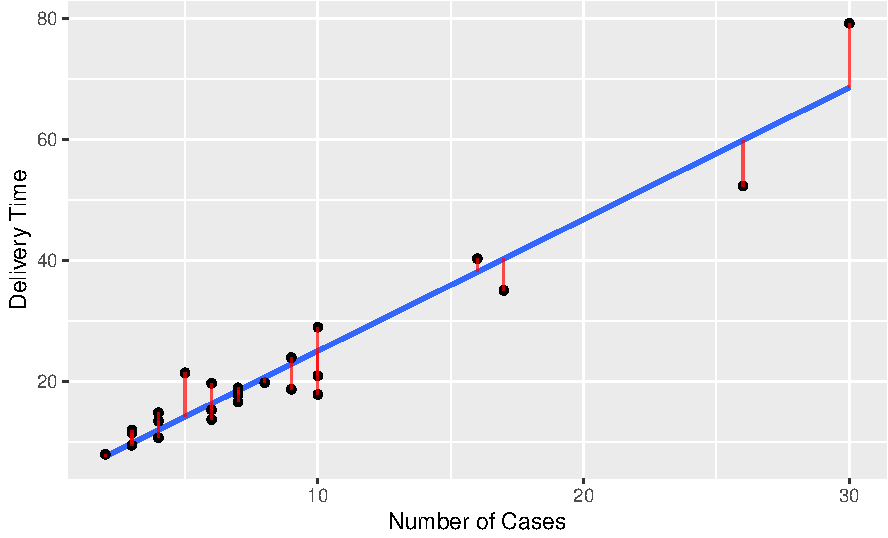
\includegraphics[width=0.7\linewidth]{regression-analysis_files/figure-latex/regplot-1} 

}

\caption{Fit and residuals}\label{fig:regplot}
\end{figure}

See Figure \ref{fig:regplot}. Each red line is \(e_i\). As we can see, \(e_i\) represents the difference between \emph{observed} response and \emph{predicted} response. A large \(\lvert e_i \rvert\) indicates a large prediction error. You can call this \(e_i\) for each \(Y_i\) by \texttt{lm()\$residuals} or \texttt{residuals()}.

\begin{Shaded}
\begin{Highlighting}[]
\NormalTok{delv_fit <-}\StringTok{ }\KeywordTok{lm}\NormalTok{(y }\OperatorTok{~}\StringTok{ }\NormalTok{x, }\DataTypeTok{data =}\NormalTok{ delv)}
\NormalTok{delv_fit}\OperatorTok{$}\NormalTok{residuals}
\CommentTok{#>      1      2      3      4      5      6      7      8      9     10 }
\CommentTok{#> -1.874  1.651  2.181  2.855 -2.628 -0.444  0.327 -0.724 10.634  7.298 }
\CommentTok{#>     11     12     13     14     15     16     17     18     19     20 }
\CommentTok{#>  2.191 -4.082  1.475  3.372  1.094  3.918 -1.028  0.446 -0.349 -5.216 }
\CommentTok{#>     21     22     23     24     25 }
\CommentTok{#> -7.182 -7.581 -4.156 -0.900 -1.275}
\end{Highlighting}
\end{Shaded}

\(\sum e_i^2\), which has been minimized in the procedure of LSE, can be used to see \emph{overall size of prediction errors}.

\BeginKnitrBlock{definition}[Residual Sum of Squares]
\protect\hypertarget{def:sse}{}{\label{def:sse} \iffalse (Residual Sum of Squares) \fi{} }\[SSE := \sum_{i = 1}^n e_i^2\]
\EndKnitrBlock{definition}

\hypertarget{residuals-and-the-variance}{%
\subsection{Residuals and the variance}\label{residuals-and-the-variance}}

\(e_i\) is a random quantity, which contains the information for \(\epsilon_i\). \(\sum e_i^2\) can give information about \(\sigma^2 = Var(\epsilon_i)\). For this, it is expected that \(e_i\) and \(\epsilon_i\) have similar feature.

\BeginKnitrBlock{lemma}
\protect\hypertarget{lem:yandbet}{}{\label{lem:yandbet} }Covriance between Y and each coefficient

\begin{enumerate}[label=(\alph*)]
  \item $Cov(\hat\beta_0, Y_i) = \bigg( \frac{1}{n} - \frac{(x_i - \overline{x})\overline{x}}{S_{XX}} \bigg)\sigma^2$ \label{itm:yandbetone}
  \item $Cov(\hat\beta_1, Y_i) = \frac{(x_i - \overline{x})}{S_{XX}}\sigma^2$ \label{itm:yandbettwo}
\end{enumerate}
\EndKnitrBlock{lemma}

\BeginKnitrBlock{proof}
\iffalse{} {Proof. } \fi{}\(\ref{itm:yandbetone}\)

\begin{equation*}
  \begin{split}
    Cov(\hat\beta_0, Y_i) & = Cov(\sum a_i Y_i, Y_i) \\
    & = \bigg( \frac{1}{n} - \frac{(x_i - \overline{x})\overline{x}}{S_{XX}} \bigg)\sigma^2
  \end{split}
\end{equation*}

\(\ref{itm:yandbettwo}\)

\begin{equation*}
  \begin{split}
    Cov(\hat\beta_1, Y_i) & = Cov(\sum b_i Y_i, Y_i) \\
    & = \frac{(x_i - \overline{x})}{S_{XX}}\sigma^2
  \end{split}
\end{equation*}
\EndKnitrBlock{proof}

\BeginKnitrBlock{proposition}[Properties of residuals]
\protect\hypertarget{prp:resprop}{}{\label{prp:resprop} \iffalse (Properties of residuals) \fi{} }Mean and variance of the residual

\begin{enumerate}[label=(\alph*)]
  \item $E(e_i) = 0$ \label{itm:respropone}
  \item $Var(e_i) \neq \sigma^2$ \label{itm:resproptwo}
  \item $\forall i \neq j : Cov(e_i, e_j) \neq 0$ \label{itm:respropthree}
\end{enumerate}
\EndKnitrBlock{proposition}

\BeginKnitrBlock{proof}
\iffalse{} {Proof. } \fi{}\(\ref{itm:respropone}\) Recall that this is the assumption of the regression model.

\(\ref{itm:resproptwo}\) Lemma \ref{lem:yandbet} implies that

\begin{equation*}
  \begin{split}
    Cov(\overline{Y}, \hat\beta_1) & = Cov(\frac{1}{n}\sum Y_i, \hat\beta_1) \\
    & = \frac{1}{n} \sum_{i = 1}^n \frac{(x_i - \overline{x})}{S_{XX}}\sigma^2 \\
    & = 0 \qquad \because \sum (x_i - \overline{x}) = 0
  \end{split}
\end{equation*}

Then

\begin{equation}
  \begin{split}
    Var(\hat{Y_i}) & = Var(\hat\beta_0 + \hat\beta_1 x_i) \\
    & = Var \bigg[ \overline{Y} + (x_i - \overline{x}) \hat\beta_1 \bigg] \qquad \because \hat\beta_0 = \overline{Y} - \hat\beta_1 \overline{x} \\
    & = Var(\overline{Y}) + (x_i - \overline{x})^2 Var(\hat\beta_1) + 2(x_i - \overline{x}) Cov(\overline{Y}, \hat\beta_1) \\
    & = \frac{\sigma^2}{n} + (x_i - \overline{x})^2\frac{\sigma^2}{S_{XX}} + 0 \\
    & = \bigg( \frac{1}{n} + \frac{(x_i - \overline{x})^2}{S_{XX}} \bigg)\sigma^2
  \end{split}
  \label{eq:predvar}
\end{equation}

From the same lemma \ref{lem:yandbet},

\begin{equation}
  \begin{split}
    Cov(Y_i, \hat{Y_i}) & = Cov(Y_i, \overline{Y} + (x_i - \overline{x}) \hat\beta_1) \\
    & = Cov(Y_i, \overline{Y}) + (x_i - \overline{x}) Cov(Y_i, \hat\beta_1) \\
    & = \frac{\sigma^2}{n} + \frac{(x_i - \overline{x})^2}{S_{XX}}\sigma^2 \qquad \because Cov(Y_i, \hat\beta_1) = \frac{(x_i - \overline{x})}{S_{XX}}\sigma^2 \\
    & = \bigg( \frac{1}{n} + \frac{(x_i - \overline{x})^2}{S_{XX}} \bigg)\sigma^2
  \end{split}
  \label{eq:yyhat}
\end{equation}

These Equations \eqref{eq:predvar} and \eqref{eq:yyhat} give that

\begin{equation}
  \begin{split}
    Var(e_i) & = Var(Y_i) + Var(\hat{Y_i}) -2Cov(Y_i, \hat{Y_i}) \\
    & = \sigma^2 + \bigg( \frac{1}{n} + \frac{(x_i - \overline{x})^2}{S_{XX}} \bigg)\sigma^2 - 2 \bigg( \frac{1}{n} + \frac{(x_i - \overline{x})^2}{S_{XX}} \bigg)\sigma^2 \\
    & = \bigg(1 - \frac{1}{n} - \frac{(x_i - \overline{x})^2}{S_{XX}} \bigg)\sigma^2 \\
    & \neq \sigma^2
  \end{split}
  \label{eq:residvar}
\end{equation}

\(\ref{itm:respropthree}\) Let \(i \neq j\). Then

\begin{equation*}
  \begin{split}
    Cov(e_i, e_j) & = Cov\Big( Y_i - (\hat\beta_0 + \hat\beta_1 x_i), Y_j - (\hat\beta_0 + \hat\beta_1 x_j) \Big) \\
    & = Cov(Y_i, Y_j) - Cov\Big(Y_i, (\hat\beta_0 + \hat\beta_1 x_j) \Big) - Cov((\hat\beta_0 + \hat\beta_1 x_i), Y_j) + Cov((\hat\beta_0 + \hat\beta_1 x_i), (\hat\beta_0 + \hat\beta_1 x_j)) \\
    & = 0 - \bigg( \frac{1}{n} - \frac{(x_i - \overline{x})\overline{x}}{S_{XX}} \bigg)\sigma^2 - \frac{(x_i - \overline{x})x_j}{S_{XX}}\sigma^2 \\
    & \qquad - \bigg( \frac{1}{n} - \frac{(x_j - \overline{x})\overline{x}}{S_{XX}} \bigg)\sigma^2 - \frac{(x_i - \overline{x})x_i}{S_{XX}}\sigma^2 \\
    & \qquad + \bigg( \frac{1}{n} + \frac{\overline{x}^2 + x_i x_j - \overline{x}(x_i + x_j)}{S_{XX}} \bigg)\sigma^2 \\
    & = - \bigg( \frac{1}{n} + \frac{\overline{x}^2 + x_i x_j - \overline{x}(x_i + x_j)}{S_{XX}} \bigg)\sigma^2 \\
    & = - \bigg( \frac{1}{n} + \frac{(x_i - \overline{x})(x_j - \overline{x})}{S_{XX}} \bigg)\sigma^2 \\
    & \neq 0
  \end{split}
\end{equation*}
\EndKnitrBlock{proof}

\hypertarget{decomposition-of-total-variability}{%
\section{Decomposition of Total Variability}\label{decomposition-of-total-variability}}

\hypertarget{total-sum-of-squares}{%
\subsection{Total sum of squares}\label{total-sum-of-squares}}

\BeginKnitrBlock{definition}[Uncorrected Total Sum of Squares]
\protect\hypertarget{def:unsst}{}{\label{def:unsst} \iffalse (Uncorrected Total Sum of Squares) \fi{} }\[SST_{uncor} := \sum_{i = 1}^n Y_i^2\]
\EndKnitrBlock{definition}

\BeginKnitrBlock{definition}[Corrected Total Sum of Squares]
\protect\hypertarget{def:sst}{}{\label{def:sst} \iffalse (Corrected Total Sum of Squares) \fi{} }\[SST := \sum_{i = 1}^n (Y_i - \overline{Y})^2\]
\EndKnitrBlock{definition}

What does this total sum of squares mean? To know this, we should know \(\overline{Y}\) first.

\begin{Shaded}
\begin{Highlighting}[]
\NormalTok{delv }\OperatorTok\StringTok{ }
\StringTok{  }\KeywordTok{ggplot}\NormalTok{(}\KeywordTok{aes}\NormalTok{(}\DataTypeTok{x =}\NormalTok{ x, }\DataTypeTok{y =}\NormalTok{ y)) }\OperatorTok{+}
\StringTok{  }\KeywordTok{geom_smooth}\NormalTok{(}\DataTypeTok{method =} \StringTok{"lm"}\NormalTok{, }\DataTypeTok{formula =}\NormalTok{ y }\OperatorTok{~}\StringTok{ }\DecValTok{1}\NormalTok{, }\DataTypeTok{se =} \OtherTok{FALSE}\NormalTok{) }\OperatorTok{+}
\StringTok{  }\KeywordTok{geom_point}\NormalTok{() }\OperatorTok{+}
\StringTok{  }\KeywordTok{labs}\NormalTok{(}
    \DataTypeTok{x =} \StringTok{"Number of Cases"}\NormalTok{,}
    \DataTypeTok{y =} \StringTok{"Delivery Time"}
\NormalTok{  )}
\end{Highlighting}
\end{Shaded}

\begin{figure}[H]

{\centering 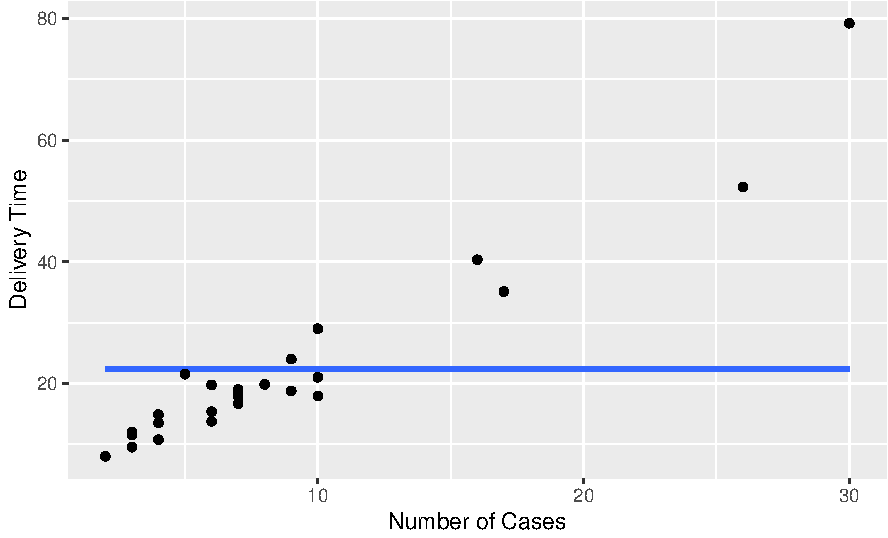
\includegraphics[width=0.7\linewidth]{regression-analysis_files/figure-latex/ybarpred-1} 

}

\caption{Regression without predictor}\label{fig:ybarpred}
\end{figure}

See Figure \ref{fig:ybarpred}. The line represents the closest line when we use only intercept term for the regression model. In other words, \emph{if we use no information for the response}, i.e.~no predictor variables, we will get just average of the response variable. Consider

\[Y_i = \beta_0 + \epsilon_i\]

Then we can get only one normal equation

\[\sum (Y_i - \hat\beta_0) = 0\]

Hence,

\[\hat\beta_0 = \frac{1}{n} \sum_{i = 1}^n Y_i \equiv \overline{Y}\]

From this fact, \(SST\) implies \textbf{total variance}.

\hypertarget{regression-sum-of-squares}{%
\subsection{Regression sum of squares}\label{regression-sum-of-squares}}

\BeginKnitrBlock{definition}[Regression Sum of Squares]
\protect\hypertarget{def:ssr}{}{\label{def:ssr} \iffalse (Regression Sum of Squares) \fi{} }\[SSR := \sum_{i = 1}^n (\hat{Y_i} - \overline{Y})^2\]
\EndKnitrBlock{definition}

This \(SSR\) compares \(\hat{Y_i}\) versus \(\overline{Y}\), computing the sum of squares for difference between predicted values from \emph{regression model} and \emph{model not using predictors}.

\hypertarget{residual-sum-of-squares}{%
\subsection{Residual sum of squares}\label{residual-sum-of-squares}}

Now consider the \emph{residual sum of squares} \(SSE\) in the definition \ref{def:sse}. As mentioned, this is related to the \emph{prediction errors}, which the regression model could not explain the data.

\hypertarget{decompsst}{%
\subsection{Decomposition of total sum of squares}\label{decompsst}}

\(SST\) can be decomposed by construction of sum of squares.

\BeginKnitrBlock{proposition}[Decomposition of SST]
\protect\hypertarget{prp:decom}{}{\label{prp:decom} \iffalse (Decomposition of SST) \fi{} }\[SST = SSR + SSE\]

where \(SST = \sum (Y_i - \overline{Y})^2\), \(SSR = \sum (\hat{Y_i} - \overline{Y})^2\), and \(SSE = \sum (Y_i - \hat{Y_i})\)
\EndKnitrBlock{proposition}

\BeginKnitrBlock{proof}
\iffalse{} {Proof. } \fi{}From the Example \ref{exm:usingnormal},

\begin{equation*}
  \begin{split}
    \sum_{i = 1}^n (Y_i - \overline{Y})^2 & = \sum_{i = 1}^n (Y_i - \hat{Y_i} + \hat{Y_i} - \overline{Y})^2 \\
    & = \sum_{i = 1}^n (Y_i - \hat{Y_i})^2 + 2 \sum_{i = 1}^n (Y_i - \hat{Y_i})(\hat{Y_i} - \overline{Y}) + \sum_{i = 1}^n (\hat{Y_i} - \overline{Y})^2 \\
    & = \sum_{i = 1}^n (Y_i - \hat{Y_i})^2 + \sum_{i = 1}^n (\hat{Y_i} - \overline{Y})^2 \qquad \because \sum (Y_i - \hat{Y_i}) = 0 \: \text{and} \: \sum (Y_i - \hat{Y_i})\hat{Y_i} = 0
  \end{split}
\end{equation*}
\EndKnitrBlock{proof}

This represents each \(SSR\) and \(SSE\) divides total variability as following.

\[\overset{SST}{\text{total variability}} = \overset{SSR}{\text{explained by regression}} + \overset{SSE}{\text{left unexplained by regression}}\]

Denote that the total variability \(SST\) is \emph{constant given data set}. If our model is good, \(SSR\) grows and \(SSE\) flattens. Thus the larger \(SSR\) is, the better. The lower \(SSE\) is, the better.

\hypertarget{coefficient-of-determination}{%
\subsection{Coefficient of determination}\label{coefficient-of-determination}}

We have discussed in the previous section \ref{decompsst} that \(SSR\) and \(SSE\) splits the total variability into \emph{explained part and not-explained part by our regression model}. Our first interest is whether the model works well for the data well, so we can think about the \emph{proportion of explained part to the total variance}. The following measure \(R^2\) computes this kind of value.

\BeginKnitrBlock{definition}[Coefficient of Determination]
\protect\hypertarget{def:rsq}{}{\label{def:rsq} \iffalse (Coefficient of Determination) \fi{} }\[R^2 := \frac{SSR}{SST} = 1 - \frac{1 - SSE}{SST}\]
\EndKnitrBlock{definition}

By construction,

\[0 \le R^2 \le 1\]

As \(R^2\) goes to \(0\), the model goes wrong. As \(R^2\) is close to \(1\), large proportion of variability has been explained. So we prefer large values rather than small.

\BeginKnitrBlock{proposition}
\protect\hypertarget{prp:rsqlin}{}{\label{prp:rsqlin} }\(R^2\) shows the strength of linear relation between two variables \(x\) and \(Y\) in the simple linear regression.

\[R^2 = \hat\rho_{XY}\]

where \(\hat\rho_{XY} := \frac{\sum (X_i - \overline{X})(Y_i - \overline{Y})}{\sqrt{\sum (X_i - \overline{X})^2} \sqrt{\sum (Y_i - \overline{Y})^2}}\) is the sample correlation coefficients
\EndKnitrBlock{proposition}

\BeginKnitrBlock{proof}
\iffalse{} {Proof. } \fi{}Note that \(\hat{Y_i} - \overline{Y} = \hat\beta_1 (x_i - \overline{x}) = \frac{S_{XY}}{S_{XX}} (x_i - \overline{x})\). Then

\begin{equation*}
  \begin{split}
    \sum (\hat{Y_i} - \overline{Y})^2 & = \frac{S_{XY}^2}{S_{XX}^2} \sum (x_i - \overline{x})^2 \\
    & = \frac{S_{XY}^2}{S_{XX}}
  \end{split}
\end{equation*}

It follows that

\begin{equation*}
  \begin{split}
    R^2 & = \frac{\sum (\hat{Y_i} - \overline{Y})^2}{\sum (Y_i - \overline{Y})^2} \\
    & = \frac{S_{XY}^2}{S_{XX}S_{YY}} \\
    & =: \hat\rho_{XY}^2
  \end{split}
\end{equation*}
\EndKnitrBlock{proof}

In this relation, we can know that \(R^2\) statistic performs as a measure of the linear relationship in the simple linear regression setting.

\hypertarget{matnot}{%
\section{Geometric Interpretations}\label{matnot}}

\hypertarget{fundamental-subspaces}{%
\subsection{Fundamental subspaces}\label{fundamental-subspaces}}

These linear algebra concepts might be more useful for \emph{multiple linear regression}, but let's briefly recap \citep{Leon:2014aa}.

\BeginKnitrBlock{definition}[Fundamental Subspaces]
\protect\hypertarget{def:subspace}{}{\label{def:subspace} \iffalse (Fundamental Subspaces) \fi{} }Let \(X \in \mathbb{R}^{n \times (p + 1)}\).

Then the Null space is defined by

\[N(X) := \{ \mathbf{b} \in \mathbb{R}^n \mid X\mathbf{b} = \mathbf{0} \}\]

The Row space is defined by

\[Row(X) := sp(\{\mathbf{r}_1, \ldots, \mathbf{r}_{p + 1} \}) \quad \text{where} \: X^T = [\mathbf{r}_1^T, \ldots, \mathbf{r}_{n}^T]\]

The Column space is defined by

\[Col(X) := sp(\{\mathbf{c}_1, \ldots, \mathbf{c}_{n} \}) \quad \text{where} \: X = [\mathbf{c}_1, \ldots, \mathbf{c}_{p + 1}]\]

The Range of \(X\) is defined by

\[R(X) := \{ \mathbf{y} \in \mathbb{R}^n \mid \mathbf{y} = X\mathbf{b} \quad \text{for some} \: \mathbf{b} \in \mathbb{R}^{p + 1} \}\]
\EndKnitrBlock{definition}

These spaces have some constructional relationship.

\BeginKnitrBlock{theorem}[Fundamental Subspaces Theorem]
\protect\hypertarget{thm:fundsub}{}{\label{thm:fundsub} \iffalse (Fundamental Subspaces Theorem) \fi{} }Let \(X \in \mathbb{R}^{n \times (p + 1)}\). Then

\[N(X) = R(X^T)^{\perp} = Col(X^T)^{\perp} = Row(X)^{\perp}\]

Transposed matrix also satisfy this.

\[N(X^T) = R(X)^{\perp} = Col(X)^{\perp}\]
\EndKnitrBlock{theorem}

\BeginKnitrBlock{proof}
\iffalse{} {Proof. } \fi{}Let \(\mathbf{a} \in N(X)\). Then \(X\mathbf{a} = \mathbf{0}\).

Let \(\mathbf{y} \in R(X^T)\). Then \(X^T \mathbf{b} = \mathbf{y}\) for some \(\mathbf{b} \in \mathbb{R}^{p + 1}\).

Choose \(\mathbf{b} \in \mathbb{R}^{p + 1}\) such that \(X^T \mathbf{b} = \mathbf{y}\). Then

\begin{equation*}
  \begin{split}
    \mathbf{0} & = X\mathbf{a} \\
    & = \mathbf{b}^T X\mathbf{a} \\
    & = \mathbf{y}^T \mathbf{a}
  \end{split}
\end{equation*}

Hence,

\[N(X) \perp R(X^T)\]

Since

\[X^T \mathbf{b} = \mathbf{c}_1 \mathbf{b} + \cdots + \mathbf{c}_{p + 1} \mathbf{b}\]

it is trivial that \(R(X) = Col(X)\) and \(R(X^T) = Col(X^T)\).

If \(\mathbf{a} \in N(X)\), then

\[
X\mathbf{a} = \begin{bmatrix}
  \mathbf{r}_1 \\
  \mathbf{r}_2 \\
  \cdots \\
  \mathbf{r}_n
\end{bmatrix} \begin{bmatrix}
  a_1 \\
  \cdots \\
  a_{p + 1}
\end{bmatrix} = \begin{bmatrix}
  0 \\
  0 \\
  \cdots \\
  0
\end{bmatrix}
\]

Thus,

\[\forall i :  \mathbf{a}^T \mathbf{r}_i = 0\]

and so

\[N(X) \subseteq Row(X)^{\perp}\]

Conversely, if \(\mathbf{a} \in Row(X)^{\perp}\), then \(\forall i : \mathbf{a}^T \mathbf{r}_i = 0\). This implies that \(X\mathbf{a} = \mathbf{0}\). Thus,

\[Row(X)^{\perp} \subseteq N(X)\]

and so

\[N(X) = Row(X)^{\perp}\]
\EndKnitrBlock{proof}

\(N(X^T) = R(X)^{\perp}\) part in Theorem \ref{thm:fundsub} will give the geometric insight to \emph{least squares solution}.

\BeginKnitrBlock{theorem}
\protect\hypertarget{thm:perpbasis}{}{\label{thm:perpbasis} }Let \(S\) be a subspace of \(\mathbb{R}^n\). Then

\[dim S + dim S^{\perp} = n\]

If \(\{ \mathbf{x}_1, \ldots, \mathbf{x}_r \}\) is a basis for \(S\) and \(\{ \mathbf{x}_{r + 1}, \ldots, \mathbf{x}_n \}\) is a basis for \(S^{\perp}\), then \(\{ \mathbf{x}_1, \ldots, \mathbf{x}_r, \mathbf{x}_{r + 1}, \ldots, \mathbf{x}_n \}\) is a basis for \(\mathbb{R}^n\).
\EndKnitrBlock{theorem}

\BeginKnitrBlock{theorem}
\protect\hypertarget{thm:dsum}{}{\label{thm:dsum} }Let \(S\) be a subspace of \(\mathbb{R}^n\). Then

\[\mathbb{R}^n = S \oplus S^{\perp}\]
\EndKnitrBlock{theorem}

\hypertarget{simple-linear-regression}{%
\subsection{Simple linear regression}\label{simple-linear-regression}}

\BeginKnitrBlock{theorem}
\protect\hypertarget{thm:projection}{}{\label{thm:projection} }Let \(S\) be a subspace of \(\mathbb{R}^n\). For each \(\mathbf{y} \in \mathbf{R}^n\), there exists a unique \(\mathbf{p} \in S\) that is closest to \(\mathbf{y}\), i.e.

\[\Vert \mathbf{y} - \mathbf{p}  \Vert > \Vert \mathbf{y} - \mathbf{\hat{y}} \Vert\]

for any \(\mathbf{p} \neq \mathbf{\hat{y}}\). Furthermore, a given vector \(\mathbf{p} \in S\) will be the closest to a given vector \(\mathbf{y} \in \mathbb{R}^n\) if and only if

\[\mathbf{y} - \mathbf{\hat{y}} \in S^{\perp}\]
\EndKnitrBlock{theorem}

Least square estimator \((\hat\beta_0, \hat\beta_1)^T\) minimizes

\begin{equation}
  \sum_{i = 1}^n (Y_i - \beta_0 - \beta_1 x_i)^2 = \Vert \mathbf{Y} - (\beta_0 \mathbf{1} + \beta_1 \mathbf{x}) \Vert^2
  \label{eq:qmatrix}
\end{equation}

with respect to \((\hat\beta_0, \hat\beta_1)^T \in \mathbb{R}^2\) (where \(\mathbf{1} := (1, 1)^T\)). Recall that the normal equation gives

\[\sum_{i = 1}^n(Y_i - \hat\beta_0 - \hat\beta_1 x_i) = \Big( \mathbf{Y} - (\hat\beta_0 \mathbf{1} + \hat\beta_1 \mathbf{x}) \Big)^T \mathbf{1} = 0\]

and

\[\sum_{i = 1}^n (Y_i - \hat\beta_0 - \hat\beta_1 x_i)x_i = \Big( \mathbf{Y} - (\hat\beta_0 \mathbf{1} + \hat\beta_1 \mathbf{x}) \Big)^T \mathbf{x} = 0\]

These two relation give

\[\mathbf{Y} - (\hat\beta_0 \mathbf{1} + \hat\beta_1 \mathbf{x}) \perp sp(\{ \mathbf{1}, \mathbf{x} \})^{\perp}\]

i.e.~\(\mathbf{\hat{Y}} = \hat\beta_0 \mathbf{1} + \hat\beta_1 \mathbf{x}\) is the projection of \(\mathbf{Y}\).

Theorem \ref{thm:projection} can give the same result.

\[\hat\beta_0 \mathbf{1} + \hat\beta_1 \mathbf{x} \in R([\mathbf{1}, \mathbf{x}])^{\perp} = sp(\{ \mathbf{1}, \mathbf{x} \})^{\perp}\]

\begin{figure}[H]

{\centering 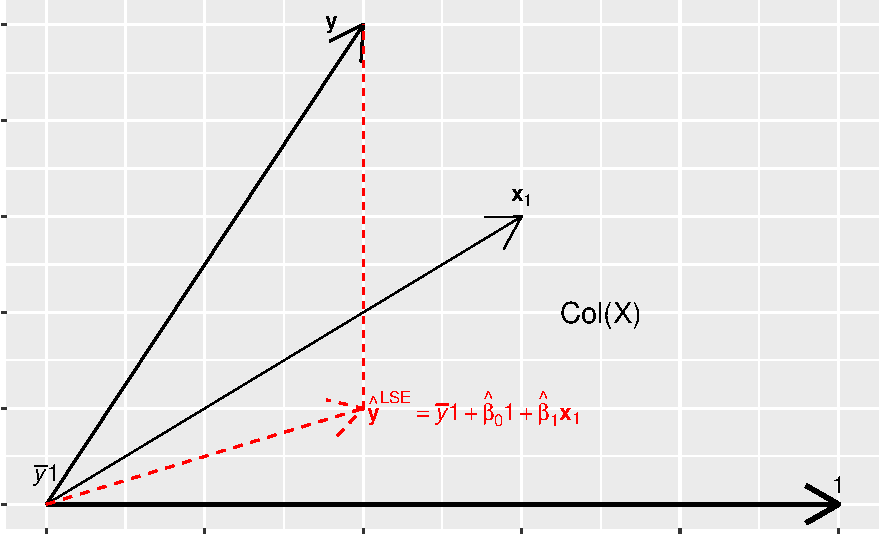
\includegraphics[width=0.7\linewidth]{regression-analysis_files/figure-latex/simpledraw-1} 

}

\caption{Geometric Illustration of Simple Linear Regression}\label{fig:simpledraw}
\end{figure}

We can see the details from Figure \ref{fig:simpledraw}. In fact, decomposition of \(SST\) and \(R^2\) are also in here.

\begin{figure}[H]

{\centering 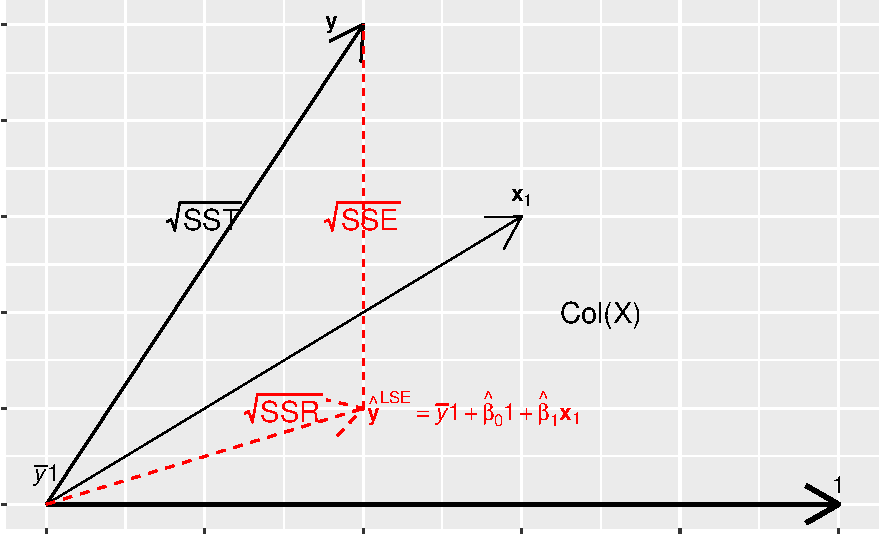
\includegraphics[width=0.7\linewidth]{regression-analysis_files/figure-latex/simpledraw2-1} 

}

\caption{Geometric Illustration of Decomposing SST}\label{fig:simpledraw2}
\end{figure}

See Figure \ref{fig:simpledraw2}.

\[
\begin{cases}
  SST = \lVert \mathbf{Y} - \overline{Y} \mathbf{1} \rVert^2 \\
  SSR = \lVert \mathbf{\hat{Y}} - \overline{Y} \mathbf{1} \rVert^2 \\
  SSE = \lVert \mathbf{Y} - \mathbf{\hat{Y}} \rVert^2
\end{cases}
\]

Pythagorean law implies that

\[SST = SSR + SSE\]

Also,

\begin{equation}
  R^2 = \frac{SSR}{SST} = cos^2\theta = \hat\rho_{XY}^2
  \label{eq:rsqcos}
\end{equation}

\hypertarget{solproj}{%
\subsection{Projection mapping}\label{solproj}}

Look again Figure \ref{fig:simpledraw}. Let \(X \equiv [\mathbf{1}, \mathbf{x}] \in \mathbb{R}^{n \times 2}\) and let \(\boldsymbol\beta \equiv (\beta_0, \beta_1)^T\). By the fundamental subspaces theorem \ref{thm:fundsub},

\[\mathbf{Y} - X\boldsymbol{\hat\beta} \in Col(X)^{\perp} = N(X^T)\]

Thus,

\begin{equation}
  X^T(\mathbf{Y} - X\boldsymbol{\hat\beta}) = \mathbf{0}
  \label{eq:projeq}
\end{equation}

This is the another representation of normal equation. Then we now have

\begin{equation*}
  \begin{split}
    & X^T\mathbf{Y} - X^TX\boldsymbol{\hat\beta} = \mathbf{0} \\
    & \Leftrightarrow X^T\mathbf{Y} = X^TX\boldsymbol{\hat\beta}
  \end{split}
\end{equation*}

If \(X^TX\) is nonsingular,

\[\boldsymbol{\hat\beta} = (X^TX)^{-1}X^T \mathbf{Y}\]

It follows that

\[\mathbf{\hat{Y}} = X\boldsymbol{\hat\beta} = X(X^TX)^{-1}X^T \mathbf{Y}\]

Combining this equation and our figure, we can know that \(X(X^TX)^{-1}X^T\) projects \(\mathbf{Y}\) from \(\mathbb{R}^n\) onto \(Col(X) = R(X)\). This is called projection operator/mapping.

\BeginKnitrBlock{definition}[Projection matrix]
\protect\hypertarget{def:projop}{}{\label{def:projop} \iffalse (Projection matrix) \fi{} }Projection operator or mapping from \(\mathbb{R}^n\) to \(W\) is written by

\[\Pi(\cdot \mid W) := X(X^TX)^{-1}X^T\]

It can also be called \textbf{\textit{Hat matrix}} and written as \(H\).
\EndKnitrBlock{definition}

As mentioned, \(X^TX\) should be invertible to get the LSE solution.

\BeginKnitrBlock{theorem}
\protect\hypertarget{thm:fullrank}{}{\label{thm:fullrank} }Let \(\mathbf{Y} = X\boldsymbol\beta\) inconsistent and let \(X \in \mathbb{R}^{n \times (p + 1)}\) with \(n > p + 1\).

If \(rank(X) = p + 1\), i.e.~full rank, then \(X^T X\) is invertible.
\EndKnitrBlock{theorem}

\BeginKnitrBlock{proof}
\iffalse{} {Proof. } \fi{}Suppose that \((X^TX)\mathbf{b} = \mathbf{0}\). Then

\[X^T (X\mathbf{b}) = \mathbf{0}\]

By the fundamental subspaces theorem \ref{thm:fundsub},

\[X\mathbf{b} \in N(X^T) = Col(X)^{\perp}\]

By construction,

\[X\mathbf{b} \in Col(X) = N(X^T)^{\perp}\]

Then

\[X\mathbf{b} \in N(X^T) \cap N(X^T)^{\perp} = \{ \mathbf{0} \}\]

It follows that

\[X\mathbf{b} = \mathbf{0}\]

If \(rank(X) = \min(n, p + 1)\), then the linear equation system has trivial solution \(\mathbf{b} = \mathbf{0}\) and so does \(X^T (X\mathbf{b}) = \mathbf{0}\). Hence, \(X^T X\) is invertible.
\EndKnitrBlock{proof}

Using projection matrix \(\Pi_W\), we can re-express each sum of squares. Recall that when we only use \(y_i\) for regression fitting, the result becomes its average. It is because \(\mathbf{Y}\) vector has been projected onto \(sp(\{ \mathbf{1} \})\) line.

\BeginKnitrBlock{remark}
\iffalse{} {Remark. } \fi{}\[\overline{Y}\mathbf{1} = \mathbf{1}(\mathbf{1}^T\mathbf{1})^{-1}\mathbf{1}^T\mathbf{Y} = \Pi_{\mathbf{1}}\mathbf{Y}\]

\[\mathbf{\hat{Y}} = X(X^TX)^{-1}X^T \mathbf{Y} = \Pi_X \mathbf{Y}\]
\EndKnitrBlock{remark}

Intuitively, every projection matrix is idempotent and symmetric. Once projected, the result is same when projecting it again.

\BeginKnitrBlock{corollary}[Sum of squares]
\protect\hypertarget{cor:projss}{}{\label{cor:projss} \iffalse (Sum of squares) \fi{} }\(\Pi_{\mathbf{1}}\) and \(\Pi_X\) can express each \(SS\) as following.

\begin{enumerate}[label=(\roman*)]
  \item $$SST = \mathbf{Y}^T (I - \Pi_{\mathbf{1}}) \mathbf{Y}$$
  \item $$SSR = \mathbf{Y}^T (\Pi_X - \Pi_{\mathbf{1}}) \mathbf{Y}$$
  \item $$SSE = \mathbf{Y}^T (I - \Pi_X) \mathbf{Y}$$
\end{enumerate}
\EndKnitrBlock{corollary}

\hypertarget{simpledist}{%
\section{Distributions}\label{simpledist}}

\hypertarget{mean-response-and-response}{%
\subsection{Mean response and response}\label{mean-response-and-response}}

We have already look at predicting each mean response and response from equation \eqref{eq:meanres} and \eqref{eq:indpred}.

\BeginKnitrBlock{theorem}[Estimation of the mean response]
\protect\hypertarget{thm:mux}{}{\label{thm:mux} \iffalse (Estimation of the mean response) \fi{} }\[\hat\mu_x \equiv \widehat{E(Y \mid x)} = \hat\beta_0 + \hat\beta_1 x\]
\EndKnitrBlock{theorem}

\BeginKnitrBlock{theorem}[(out of sample) Prediction of a response]
\protect\hypertarget{thm:yhatx}{}{\label{thm:yhatx} \iffalse ((out of sample) Prediction of a response) \fi{} }\[\hat{Y_x}  = \hat\beta_0 + \hat\beta_1 x\]
\EndKnitrBlock{theorem}

Recall that predicting \ref{thm:mux} targets at

\[\mu_x \equiv E(Y \mid x) = \beta_0 + \beta_1 x\]

which have been assumed to be true model. On the other hand, predicting \ref{thm:yhatx} targets at

\[Y = \beta_0 + \beta_1 + \epsilon_x\]

The linearity is not true in reality. So the errors caused by modeling linear model are included in \(\epsilon_x\). This error term makes difference between properties of \ref{thm:mux} and \ref{thm:yhatx}.

To derive their distribution and see the difference, we additionaly assume Normality, i.e.

\[\epsilon_i \stackrel{iid}{\sim} N(0, \sigma^2)\]

\hypertarget{simplebdist}{%
\subsection{Regression coefficients}\label{simplebdist}}

Under Normality, we have

\[Y_i \stackrel{indep}{\sim} N(\beta_0 + \beta_1 x_i, \sigma^2)\]

Then

\[
\mathbf{Y} = \begin{bmatrix}
  Y_1 \\
  Y_2 \\
  \vdots \\
  Y_n
\end{bmatrix} \sim MVN_n\Bigg( \boldsymbol\mu \equiv \begin{bmatrix}
  \beta_0 + \beta_1 x_1 \\
  \beta_0 + \beta_1 x_2 \\
  \vdots \\
  \beta_0 + \beta_1 x_n
\end{bmatrix}, \Sigma \equiv \sigma^2 I = \begin{bmatrix}
  \sigma^2 & 0 & \cdots & 0 \\
  0 & \sigma^2 & \cdots & 0 \\
  \vdots & \vdots & \vdots & \vdots \\
  0 & 0 & 0 & \sigma^2
\end{bmatrix} \Bigg)
\]

Write \(\boldsymbol{\hat\beta} = (\hat\beta_0, \hat\beta_1)^T\). From Lemma \ref{lem:linbet},

\[\hat\beta_0 = \mathbf{a}^T\mathbf{Y}\]

where \(\mathbf{a} = (a_1, \ldots, a_n)^T \in \mathbb{R}^n\) with \(a_i = \bigg( \frac{1}{n} - \frac{(x_i - \overline{x})\overline{x}}{S_{XX}} \bigg)\)

and

\[\hat\beta_1 = \mathbf{b}^T\mathbf{Y}\]

where \(\mathbf{b} = (b_1, \ldots, b_n)^T \in \mathbb{R}^n\) with \(b_i = \frac{(x_i - \overline{x})}{S_{XX}}\).

Let

\[
A = \begin{bmatrix}
  \mathbf{a}^T \\ \hline
  \mathbf{b}^T
\end{bmatrix} \in \mathbb{R}^{2 \times n}
\]

Then

\[
\boldsymbol{\hat\beta} = A\mathbf{Y}
\]

Linearity of the multivariate normal distribution, Proposition \ref{prp:ue} and \ref{prp:vb} imply that

\begin{equation}
  \boldsymbol{\hat\beta} = \begin{bmatrix}
    \hat\beta_0 \\ \hline
    \hat\beta_1
  \end{bmatrix} \sim MVN \bigg( A\boldsymbol\mu = \begin{bmatrix}
    \beta_0 \\ \hline
    \beta_1
  \end{bmatrix},
  A\Sigma A^T = \sigma^2 AA^T = \begin{bmatrix}
    \bigg( \frac{1}{n} + \frac{\overline{x}^2}{S_{XX}} \bigg)\sigma^2 & - \frac{\overline{x}}{S_{XX}}\sigma^2 \\ \hline
    - \frac{\overline{x}}{S_{XX}}\sigma^2 & \frac{\sigma^2}{S_{XX}}
  \end{bmatrix} \bigg)
  \label{eq:b01mvn}
\end{equation}

Since the joint random vector follows multivariate normal distribution, each \emph{partitioned subset follow normal}. For this theorem, see \citet{Johnson:2013aa}. Hence, we finally get the following result.

\BeginKnitrBlock{theorem}[Distributions of regression coefficients]
\protect\hypertarget{thm:b01dist}{}{\label{thm:b01dist} \iffalse (Distributions of regression coefficients) \fi{} }Each regression coefficient follows Normal distribution.

\[\hat\beta_0 \sim N \bigg( \beta_0, \bigg( \frac{1}{n} + \frac{\overline{x}^2}{S_{XX}} \bigg)\sigma^2 \bigg)\]

\[\hat\beta_1 \sim N \bigg( \beta_1, \frac{\sigma^2}{S_{XX}} \bigg)\]
\EndKnitrBlock{theorem}

\hypertarget{mean-response}{%
\subsection{Mean response}\label{mean-response}}

In simple linear regression setting, we assume \(\mu_x = E(Y \mid x) = \beta_0 + \beta_1 x\) is true.

\begin{Shaded}
\begin{Highlighting}[]
\NormalTok{delv }\OperatorTok\StringTok{ }
\StringTok{  }\KeywordTok{ggplot}\NormalTok{(}\KeywordTok{aes}\NormalTok{(}\DataTypeTok{x =}\NormalTok{ x, }\DataTypeTok{y =}\NormalTok{ y)) }\OperatorTok{+}
\StringTok{  }\KeywordTok{geom_smooth}\NormalTok{(}\DataTypeTok{method =} \StringTok{"lm"}\NormalTok{) }\OperatorTok{+}
\StringTok{  }\KeywordTok{geom_point}\NormalTok{(}\DataTypeTok{alpha =} \FloatTok{.7}\NormalTok{) }\OperatorTok{+}
\StringTok{  }\KeywordTok{labs}\NormalTok{(}
    \DataTypeTok{x =} \StringTok{"Number of Cases"}\NormalTok{,}
    \DataTypeTok{y =} \StringTok{"Delivery Time"}
\NormalTok{  )}
\end{Highlighting}
\end{Shaded}

\begin{figure}[H]

{\centering 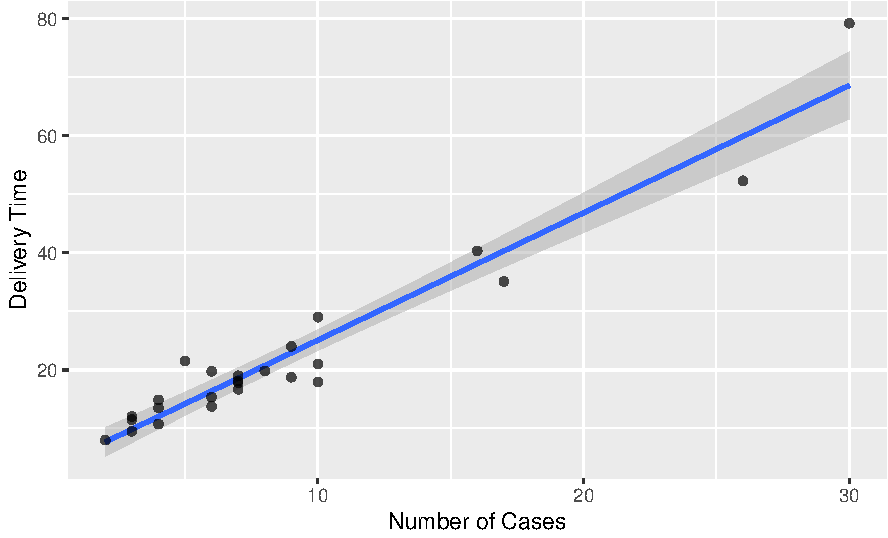
\includegraphics[width=0.7\linewidth]{regression-analysis_files/figure-latex/smoothline-1} 

}

\caption{Mean response and its standard deviation}\label{fig:smoothline}
\end{figure}

For example, in the Figure \ref{fig:smoothline}, the blue line indicates \(E(Y \mid X = x)\) for each point \(x\). Without fitting using \texttt{lm()}, \texttt{geom\_smooth(method\ =\ "lm")} let us visualize the fitted line. Since the default method is not the linear regression, the \texttt{method} option should be specified.

\begin{Shaded}
\begin{Highlighting}[]
\NormalTok{delv }\OperatorTok\StringTok{ }
\StringTok{  }\KeywordTok{mutate}\NormalTok{(}\DataTypeTok{eyx =} \KeywordTok{predict}\NormalTok{(delv_fit, }\DataTypeTok{newdata =} \KeywordTok{data.frame}\NormalTok{(}\DataTypeTok{x =}\NormalTok{ x)))}
\CommentTok{#> # A tibble: 25 x 3}
\CommentTok{#>       y     x   eyx}
\CommentTok{#>   <dbl> <dbl> <dbl>}
\CommentTok{#> 1  16.7     7 18.6 }
\CommentTok{#> 2  11.5     3  9.85}
\CommentTok{#> 3  12.0     3  9.85}
\CommentTok{#> 4  14.9     4 12.0 }
\CommentTok{#> 5  13.8     6 16.4 }
\CommentTok{#> 6  18.1     7 18.6 }
\CommentTok{#> # ... with 19 more rows}
\end{Highlighting}
\end{Shaded}

We have already seen in section \ref{simplebdist} that the estimators \(\hat\beta_0\) and \(\hat\beta_1\) are random variables. So \(\hat\mu_x\) is. In fact, the ribbon of the line in Figure \ref{fig:smoothline} represents upper and lower confidence limits on mean response. In the later section, we get to know that it is \(+ t(n - 2)\widehat{SE}(\hat\mu_x)\) and \(- t(n - 2) \widehat{SE}(\hat\mu_x)\). It can be drawn by default with the option of the \texttt{geom\_smooth(se\ =\ TRUE)}.

\BeginKnitrBlock{theorem}[Distribution of mean response estimator]
\protect\hypertarget{thm:mrdist}{}{\label{thm:mrdist} \iffalse (Distribution of mean response estimator) \fi{} }\(\hat\mu_x\) is also Normally distributed.

\[\hat\mu_x \sim N\bigg( \mu_x, \sigma^2\bigg( \frac{1}{n} + \frac{(x - \overline{x})^2}{S_{XX}} \bigg) \bigg)\]
\EndKnitrBlock{theorem}

\BeginKnitrBlock{proof}
\iffalse{} {Proof. } \fi{}Since \(\hat\mu_x = \hat\beta_0 + \hat\beta_1 x\) is the linear combination of \((\hat\beta_0, \hat\beta_1)^T\),

\[\hat\mu_x \sim N\Big(E(\hat\mu_x), Var(\hat\mu_x)\Big)\]

From Theorem \ref{thm:b01dist},

\[E(\hat\mu_x) = E(\hat\beta_0) + E(\hat\beta_1)x = \beta_0 + \beta_1x \equiv \mu_x\]

and from Proposition \ref{prp:vb}

\begin{equation*}
  \begin{split}
    Var(\hat\mu_x) & = Var(\hat\beta_0 + \hat\beta_1 x) \\
    & = Var(\hat\beta_0) + x^2Var(\hat\beta_1) + 2xCov(\hat\beta_0, \hat\beta_1) \\
    & = \bigg( \frac{1}{n} + \frac{\overline{x}^2}{S_{XX}} \bigg)\sigma^2 + \frac{x^2\sigma^2}{S_{XX}} - \frac{2\overline{x}x\sigma^2}{S_{XX}} \\
    & = \sigma^2\bigg(\frac{1}{n} + \frac{(x - \overline{x})^2}{S_{XX}} \bigg)
  \end{split}
\end{equation*}
\EndKnitrBlock{proof}

\BeginKnitrBlock{corollary}
\protect\hypertarget{cor:mrdiff}{}{\label{cor:mrdiff} }\[\hat\mu_x - \mu_x \sim N\bigg( 0, \sigma^2\bigg( \frac{1}{n} + \frac{(x - \overline{x})^2}{S_{XX}} \bigg) \bigg)\]
\EndKnitrBlock{corollary}

Denote that in both Theorem \ref{thm:mrdist} and Corollary \ref{cor:mrdiff}, \(\sigma^2\) is parameter. So to use \(SE(\hat\mu_x) = \sqrt{Var(\hat\mu_x)}\) in practice we plug in its estimator, usually Equation \eqref{eq:siglse}.

\BeginKnitrBlock{corollary}[Standard error of mean response estimator]
\protect\hypertarget{cor:mrse}{}{\label{cor:mrse} \iffalse (Standard error of mean response estimator) \fi{} }\[\widehat{SE}(\hat\mu_x) = \hat\sigma \sqrt{\bigg( \frac{1}{n} + \frac{(x - \overline{x})^2}{S_{XX}} \bigg)}\]

where \(\hat\sigma^2 = MSE\)
\EndKnitrBlock{corollary}

\hypertarget{response}{%
\subsection{Response}\label{response}}

Our goal is to predict each response at each point, i.e.~\(Y_x = \beta_0 + \beta_1 x + \epsilon_x\). \(\epsilon_x \sim N(0, \sigma^2)\) is independent of the given data (\(\epsilon_1, \ldots, \epsilon_n\)). In this sense, this prediction is called \emph{out of sample prediction}. This setting makes difference between the \emph{residuals, which are correlated to the data}. See Proposition \ref{prp:resprop} for this. This is occurred because each \(\hat\beta_0\) and \(\hat\beta_1\) is linear combination of \(Y_1, \ldots, Y_n\), not \(Y_x\).

While \(Cov(Y_i, \hat{Y_i}) > 0, i = 1, \ldots, n\) (See Equation \eqref{eq:yyhat}), in case of out-of-sample \(Y_x\),

\[Cov(Y_x, \hat{Y_x}) = Cov(Y_x, \hat\beta_0 + \hat\beta_1 x) = 0\]

Hence, arithmetically, this \emph{out of sample prediction becomes to have larger standard error}.

\BeginKnitrBlock{proposition}[Joint distribution of coefficients and error term]
\protect\hypertarget{prp:bepsmvn}{}{\label{prp:bepsmvn} \iffalse (Joint distribution of coefficients and error term) \fi{} }\((\hat\beta_0, \hat\beta_1, \epsilon_x)^T\) is Normally distributed.
\EndKnitrBlock{proposition}

\BeginKnitrBlock{proof}
\iffalse{} {Proof. } \fi{}Want 1: \((\hat\beta_0, \hat\beta_1)^T \perp\!\!\!\perp \epsilon_x\)

We have

\begin{equation}
  \begin{split}
    Cov((\hat\beta_0, \hat\beta_1)^T, \epsilon_x) & = \Big[Cov(\hat\beta_i, \epsilon_x) \Big]_{2 \times 1} \\
    & = \bigg[Cov\bigg(\sum_{i = 1}^n k_i Y_i, \epsilon_x \bigg) \bigg]_{2 \times 1} \qquad k_i = \text{each linear coefficient for}\: \hat\beta_0, \hat\beta_1 \\
    & = \mathbf{0}
  \end{split}
  \label{eq:betaepsind}
\end{equation}

From Equation \eqref{eq:b01mvn},

\[(\hat\beta_0, \hat\beta_1)^T \sim MVN\]

and from assumption,

\[\epsilon_x \sim N(0, \sigma^2)\]

It follows from Equation \eqref{eq:betaepsind} that (\citet{Johnson:2013aa})

\[(\hat\beta_0, \hat\beta_1)^T \perp\!\!\!\perp \epsilon_x\]

Want 2: \((\hat\beta_0, \hat\beta_1, \epsilon_x)^T \sim MVN\)

From independency, we have (\citet{Johnson:2013aa})

\[
\begin{bmatrix}
  \hat\beta_0 \\
  \hat\beta_1 \\ \hline
  \epsilon_x
\end{bmatrix} \sim MVN_{2 + 1} \bigg( \begin{bmatrix}
  \beta_0 \\
  \beta_1 \\ \hline
  0
\end{bmatrix}, \left[
  \begin{array}{c|c}
    Cov(\boldsymbol{\hat\beta}) \in \mathbb{R}^{2 \times 2} & \mathbf{0} \in \mathbb{R}^2 \\ \hline
    \mathbf{0}^T \in \mathbb{R}^{2 \times 1} & \sigma^2
  \end{array}
\right] \bigg)
\]
\EndKnitrBlock{proof}

This proposition gives clue to distribution of prediction error.

\BeginKnitrBlock{theorem}[Distribution of out-of-sample prediction error]
\protect\hypertarget{thm:preddist}{}{\label{thm:preddist} \iffalse (Distribution of out-of-sample prediction error) \fi{} }Out of sample prediction error \(\hat{Y_x} - Y_x\) is Normally distributed

\[\hat{Y_x} - Y_x \sim N\bigg( 0, \sigma^2 \bigg( 1 + \frac{1}{n} + \frac{(x - \overline{x})^2}{S_{XX}} \bigg) \bigg)\]
\EndKnitrBlock{theorem}

\BeginKnitrBlock{proof}
\iffalse{} {Proof. } \fi{}Note that

\begin{equation*}
  \begin{split}
    \hat{Y_x} - Y_x & = (\hat\beta_0 + \hat\beta_1 x) - (\beta_0 + \beta_1 x + \epsilon_x) \\
    & = [1, x, -1] (\hat\beta_0, \hat\beta_1, \epsilon_x)^T - \beta_0 - \beta_1 x
  \end{split}
\end{equation*}

i.e.~\(\hat{Y_x} - Y_x\) is a linear combination of \((\hat\beta_0, \hat\beta_1, \epsilon_x)^T\). From prosition \ref{prp:bepsmvn},

\begin{equation}
  \begin{split}
    \hat{Y_x} - Y_x & \sim MVN \Bigg( [1, x, -1]\begin{bmatrix}
    \beta_0 \\
    \beta_1 \\
    0
    \end{bmatrix} - \beta_0 - \beta_1 x,
    [1, x, -1]
    \left[
      \begin{array}{c|c}
        Cov(\boldsymbol{\hat\beta}) \in \mathbb{R}^{2 \times 2} & \mathbf{0} \in \mathbb{R}^2 \\ \hline
        \mathbf{0}^T \in \mathbb{R}^{2 \times 1} & \sigma^2
      \end{array}
    \right]
    \begin{bmatrix}
      1 \\
      x \\
      -1
    \end{bmatrix}
     \Bigg) \\
    & \stackrel{d}{=} MVN \bigg( 0, \sigma^2\bigg( \frac{1}{n} + \frac{\overline{x}^2}{S_{XX}} - 2 \frac{\overline{x}x}{S_{XX}} + \frac{x^2}{S_{XX}} \bigg) + 1 \bigg) \\
    & \stackrel{d}{=} MVN \bigg( 0, \sigma^2\bigg( 1 + \frac{1}{n} + \frac{(x - \overline{x})^2}{S_{XX}} \bigg) \bigg)
  \end{split}
  \label{eq:prederrmvn}
\end{equation}
\EndKnitrBlock{proof}

Now we know the standard error of this out-of-sample prediction error.

\[SE(\hat{Y_x} - Y_x) = \sigma \sqrt{\bigg( 1 + \frac{1}{n} + \frac{(x - \overline{x})^2}{S_{XX}} \bigg)}\]

We can see this standard error is \emph{always larger than of mean response estimator} due to \(1\) in the bracket, i.e.~\(\sigma^2\). As mentioned, this is due to \(\epsilon\) term. When we estimate or predict the mean response the model have been assumed to be true. In this out-of-sample prediction setting, however, the model can be wrong. This assumption error is also included in \(\epsilon\) term and it is called \emph{irreducible error}, which cannot be reduced anymore.

\BeginKnitrBlock{remark}
\iffalse{} {Remark. } \fi{}\[SE(\hat\mu_x - \mu_x) < SE(\hat{Y_x} - Y_x)\]
\EndKnitrBlock{remark}

It might be more clear if we see the inequality in the above remark. We know the fact that \(\hat{Y_x}\) and \(Y_x\) are uncorrelated in this out-of-sample setting. \(Y_x\) is random variable, while \(\mu_x\) is constant. Then we can re-express the inequality as

\[SE(\hat\mu_x) < SE(\hat{Y_x}) + SE(Y_x)\]

Actually, both \(\hat\mu_x\) and \(\hat{Y_x}\) are estimated as \(\hat\beta_0 + \hat\beta_1 x\). Thus, \(SE(Y_x) = \sigma^2\) makes out-of-sample more noisy.

To use standard error practically, we use \(\hat\sigma^2\) as in corollary \ref{cor:mrse}.

\BeginKnitrBlock{corollary}[Standard error of out-of-sample prediction error]
\protect\hypertarget{cor:predse}{}{\label{cor:predse} \iffalse (Standard error of out-of-sample prediction error) \fi{} }\[\widehat{SE}(\hat{Y_x} - Y_x) = \hat\sigma \sqrt{\bigg( 1 + \frac{1}{n} + \frac{(x - \overline{x})^2}{S_{XX}} \bigg)}\]

where \(\hat\sigma^2 = MSE\)
\EndKnitrBlock{corollary}

\hypertarget{statistical-inference}{%
\section{Statistical Inference}\label{statistical-inference}}

Based on each distribution of estimator in section \ref{simpledist}, we can construct various inferece for each

\begin{itemize}
\tightlist
\item
  \(\beta_0\)
\item
  \(\beta_1\)
\item
  \(\mu_x\)
\item
  \(Y_x\)
\item
  \(\sigma^2\)
\end{itemize}

We can get the standard error for each coefficient through \texttt{summary()} function.

\begin{Shaded}
\begin{Highlighting}[]
\KeywordTok{summary}\NormalTok{(delv_fit)}
\CommentTok{#> }
\CommentTok{#> Call:}
\CommentTok{#> lm(formula = y ~ x, data = delv)}
\CommentTok{#> }
\CommentTok{#> Residuals:}
\CommentTok{#>    Min     1Q Median     3Q    Max }
\CommentTok{#> -7.581 -1.874 -0.349  2.181 10.634 }
\CommentTok{#> }
\CommentTok{#> Coefficients:}
\CommentTok{#>             Estimate Std. Error t value Pr(>|t|)    }
\CommentTok{#> (Intercept)    3.321      1.371    2.42    0.024 *  }
\CommentTok{#> x              2.176      0.124   17.55  8.2e-15 ***}
\CommentTok{#> ---}
\CommentTok{#> Signif. codes:  0 '***' 0.001 '**' 0.01 '*' 0.05 '.' 0.1 ' ' 1}
\CommentTok{#> }
\CommentTok{#> Residual standard error: 4.18 on 23 degrees of freedom}
\CommentTok{#> Multiple R-squared:  0.93,   Adjusted R-squared:  0.927 }
\CommentTok{#> F-statistic:  308 on 1 and 23 DF,  p-value: 8.22e-15}
\end{Highlighting}
\end{Shaded}

Or more state-or-art way, \texttt{broom:tidy()} function has a method for each model object to make tidy data: \texttt{tibble}.

\begin{Shaded}
\begin{Highlighting}[]
\NormalTok{broom}\OperatorTok{::}\KeywordTok{tidy}\NormalTok{(delv_fit)}
\CommentTok{#> # A tibble: 2 x 5}
\CommentTok{#>   term        estimate std.error statistic  p.value}
\CommentTok{#>   <chr>          <dbl>     <dbl>     <dbl>    <dbl>}
\CommentTok{#> 1 (Intercept)     3.32     1.37       2.42 2.37e- 2}
\CommentTok{#> 2 x               2.18     0.124     17.5  8.22e-15}
\end{Highlighting}
\end{Shaded}

\hypertarget{confidence-interval}{%
\subsection{Confidence interval}\label{confidence-interval}}

Consider standardization.

\[\frac{\hat\theta - \theta}{SE(\hat\theta)}\]

Each \(SE\) includes \(\sigma^2\) as we have already seen. First think about \textbf{known} \(\sigma^2\) setting. All three estimators follow Normal distribution, and \(SE\) is constant by our the setting. Then we can construct each confidence interval as

\[\hat\theta \pm z_{\frac{\alpha}{2}} SE(\hat\theta)\]

\begin{figure}[H]

{\centering 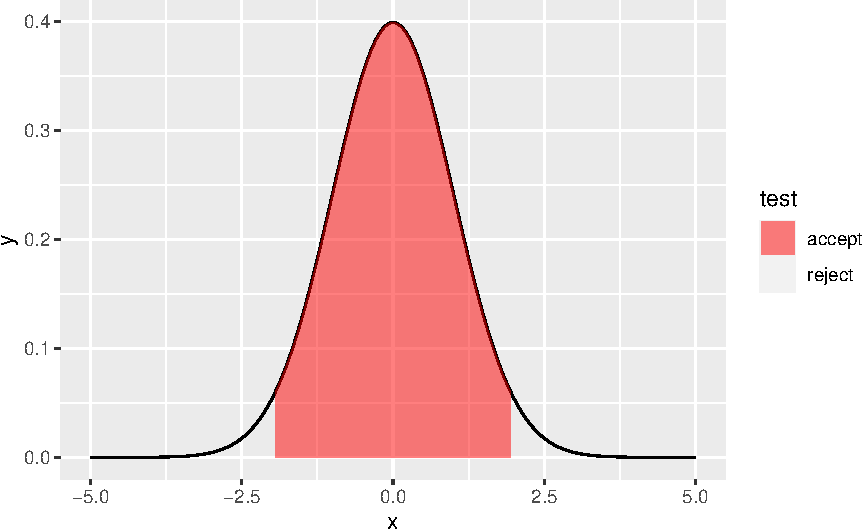
\includegraphics[width=0.7\linewidth]{regression-analysis_files/figure-latex/estci-1} 

}

\caption{Confidence Interval when $\sigma^2$ is known}\label{fig:estci}
\end{figure}

Now just plug in the results of section \ref{simpledist}. For each regression coefficient,

\BeginKnitrBlock{proposition}[Confidence intervals on $\beta$]
\protect\hypertarget{prp:betaci}{}{\label{prp:betaci} \iffalse (Confidence intervals on \(\beta\)) \fi{} }With known \(\sigma^2\), \((1 - \alpha)100 \%\) confidence intervals on \(\beta_0\) and \(\beta_1\) are given as

\[\beta_0 : \quad \hat\beta_0 \pm z_{\frac{\alpha}{2}} \sqrt{\bigg( \frac{1}{n} + \frac{\overline{x}^2}{S_{XX}} \bigg) \sigma^2}\]

\[\beta_1 : \quad \hat\beta_1 \pm z_{\frac{\alpha}{2}} \sqrt{\frac{\sigma^2}{S_{XX}}}\]
\EndKnitrBlock{proposition}

\BeginKnitrBlock{proposition}[Confidence interval on $\hat\mu_x$]
\protect\hypertarget{prp:mrci}{}{\label{prp:mrci} \iffalse (Confidence interval on \(\hat\mu_x\)) \fi{} }With known \(\sigma^2\), \((1 - \alpha)100 \%\) confidence interval on \(\hat\mu_x\) is given as

\[\mu_x : \quad \hat\mu_x \pm z_{\frac{\alpha}{2}} \sqrt{\sigma^2 \bigg( \frac{1}{n} + \frac{(x - \overline{x})^2}{S_{xx}} \bigg)}\]
\EndKnitrBlock{proposition}

In practice, however, we do not know \(\sigma^2\). In this case, we replace \(\sigma^2\) with \(\hat\sigma^2 = \frac{1}{n - 2}\sum\limits_{i = 1}^n (\hat{Y_i} - Y_i)^2 = MSE\). Then

\[\frac{\hat\theta - \theta}{\widehat{SE}} = \frac{\frac{\hat\theta - \theta}{\sqrt{Var = \sigma^2(\cdot)}}}{\sqrt{\frac{\frac{SSE}{\sigma^2}}{n - 2}\bigg( \cdot \bigg)}} =  \frac{\frac{\hat\theta - \theta}{\sqrt{Var = \sigma^2}} \sim N(0, 1)}{\sqrt{\frac{\frac{SSE}{\sigma^2} \sim \chi^2(n - 2)}{n - 2}}} \sim t(n - 2)\]

Thus, we need to replace \(z_{\frac{\alpha}{2}}\) with \(t_{\frac{\alpha}{2}}(n - 2)\).

\BeginKnitrBlock{proposition}[Confidence intervals on $\beta$ when unknown $\sigma^2$]
\protect\hypertarget{prp:betaci2}{}{\label{prp:betaci2} \iffalse (Confidence intervals on \(\beta\) when unknown \(\sigma^2\)) \fi{} }With unknown \(\sigma^2\), \((1 - \alpha)100 \%\) confidence intervals on \(\beta_0\) and \(\beta_1\) are given as

\[\beta_0 : \quad \hat\beta_0 \pm t_{\frac{\alpha}{2}}(n - 2) \sqrt{\bigg( \frac{1}{n} + \frac{\overline{x}^2}{S_{XX}} \bigg) \hat\sigma^2}\]

\[\beta_1 : \quad \hat\beta_1 \pm t_{\frac{\alpha}{2}}(n - 2) \sqrt{\frac{\hat\sigma^2}{S_{XX}}}\]

where \(\hat\sigma^2 = MSE\)
\EndKnitrBlock{proposition}

Here we can estimate the intervals. Basically, \texttt{confint()} function gives this interval.

\begin{Shaded}
\begin{Highlighting}[]
\KeywordTok{confint}\NormalTok{(delv_fit, }\DataTypeTok{level =} \FloatTok{.95}\NormalTok{)}
\CommentTok{#>             2.5 % 97.5 %}
\CommentTok{#> (Intercept) 0.484   6.16}
\CommentTok{#> x           1.920   2.43}
\end{Highlighting}
\end{Shaded}

\BeginKnitrBlock{proposition}[Confidence interval on $\hat\mu_x$ when unknown $\sigma^2$]
\protect\hypertarget{prp:mrci2}{}{\label{prp:mrci2} \iffalse (Confidence interval on \(\hat\mu_x\) when unknown \(\sigma^2\)) \fi{} }With unknown \(\sigma^2\), \((1 - \alpha)100 \%\) confidence interval on \(\hat\mu_x\) is given as

\[\mu_x : \quad \hat\mu_x \pm t_{\frac{\alpha}{2}}(n - 2) \sqrt{\hat\sigma^2 \bigg( \frac{1}{n} + \frac{(x - \overline{x})^2}{S_{xx}} \bigg)}\]

where \(\hat\sigma^2 = MSE\)
\EndKnitrBlock{proposition}

\texttt{predict()} provides options for this confidence interval. Specify \texttt{interval\ =\ "confidence"}. This argument has three option.

\begin{enumerate}
\def\labelenumi{\arabic{enumi}.}
\tightlist
\item
  \texttt{"none"}: just compute fitted value, by default.
\item
  \texttt{"confidence"}: confidence interval of mean response
\item
  \texttt{"prediction"}: prediction interval of out-of-sample prediction
\end{enumerate}

Default \texttt{level} is \texttt{0.95}.

\begin{Shaded}
\begin{Highlighting}[]
\KeywordTok{predict}\NormalTok{(delv_fit, }\DataTypeTok{interval =} \StringTok{"confidence"}\NormalTok{, }\DataTypeTok{level =} \FloatTok{.95}\NormalTok{) }\OperatorTok\StringTok{ }\KeywordTok{tbl_df}\NormalTok{()}
\CommentTok{#> # A tibble: 25 x 3}
\CommentTok{#>     fit   lwr   upr}
\CommentTok{#>   <dbl> <dbl> <dbl>}
\CommentTok{#> 1 18.6  16.8   20.3}
\CommentTok{#> 2  9.85  7.57  12.1}
\CommentTok{#> 3  9.85  7.57  12.1}
\CommentTok{#> 4 12.0   9.91  14.1}
\CommentTok{#> 5 16.4  14.5   18.2}
\CommentTok{#> 6 18.6  16.8   20.3}
\CommentTok{#> # ... with 19 more rows}
\end{Highlighting}
\end{Shaded}

\hypertarget{prediction-interval}{%
\subsection{Prediction interval}\label{prediction-interval}}

One proceeds in a similar way for out-of-sample \(Y_x\).

\BeginKnitrBlock{proposition}[Prediction interval on $\hat{Y_x}$]
\protect\hypertarget{prp:predci}{}{\label{prp:predci} \iffalse (Prediction interval on \(\hat{Y_x}\)) \fi{} }With known \(\sigma^2\), \((1 - \alpha)100 \%\) confidence interval on \(\hat\mu_x\) is given as

\[Y_x : \quad \hat{Y_x} \pm z_{\frac{\alpha}{2}} \sqrt{\sigma^2 \bigg( 1 + \frac{1}{n} + \frac{(x - \overline{x})^2}{S_{xx}} \bigg)}\]
\EndKnitrBlock{proposition}

Also, with unknown \(\sigma^2\),

\BeginKnitrBlock{proposition}[Prediction interval on $\hat{Y_x}$ when unknown $\sigma^2$]
\protect\hypertarget{prp:predci2}{}{\label{prp:predci2} \iffalse (Prediction interval on \(\hat{Y_x}\) when unknown \(\sigma^2\)) \fi{} }With unknown \(\sigma^2\), \((1 - \alpha)100 \%\) confidence interval on \(\hat\mu_x\) is given as

\[Y_x : \quad \hat{Y_x} \pm t_{\frac{\alpha}{2}}(n - 2) \sqrt{\hat\sigma^2 \bigg( 1 + \frac{1}{n} + \frac{(x - \overline{x})^2}{S_{xx}} \bigg)}\]

where \(\hat\sigma^2 = MSE\)
\EndKnitrBlock{proposition}

Since this is out-of-sample setting, we should also give \texttt{newdata} option. Otherwise, we will get warning message. Denote that this argument only receive \texttt{data.frame} object with same element names.

\begin{Shaded}
\begin{Highlighting}[]
\KeywordTok{predict}\NormalTok{(delv_fit, }\DataTypeTok{newdata =} \KeywordTok{data.frame}\NormalTok{(}\DataTypeTok{x =} \DecValTok{31}\OperatorTok{:}\DecValTok{35}\NormalTok{), }\DataTypeTok{interval =} \StringTok{"prediction"}\NormalTok{, }\DataTypeTok{level =} \FloatTok{.95}\NormalTok{)}
\CommentTok{#>    fit  lwr  upr}
\CommentTok{#> 1 70.8 60.3 81.3}
\CommentTok{#> 2 73.0 62.3 83.6}
\CommentTok{#> 3 75.1 64.3 85.9}
\CommentTok{#> 4 77.3 66.4 88.3}
\CommentTok{#> 5 79.5 68.4 90.6}
\end{Highlighting}
\end{Shaded}

\hypertarget{hypothesis-testing}{%
\subsection{Hypothesis testing}\label{hypothesis-testing}}

Look again the output of \texttt{summary.lm()} and \texttt{broom::tidy.lm()}.

\begin{Shaded}
\begin{Highlighting}[]
\KeywordTok{summary}\NormalTok{(delv_fit)}
\CommentTok{#> }
\CommentTok{#> Call:}
\CommentTok{#> lm(formula = y ~ x, data = delv)}
\CommentTok{#> }
\CommentTok{#> Residuals:}
\CommentTok{#>    Min     1Q Median     3Q    Max }
\CommentTok{#> -7.581 -1.874 -0.349  2.181 10.634 }
\CommentTok{#> }
\CommentTok{#> Coefficients:}
\CommentTok{#>             Estimate Std. Error t value Pr(>|t|)    }
\CommentTok{#> (Intercept)    3.321      1.371    2.42    0.024 *  }
\CommentTok{#> x              2.176      0.124   17.55  8.2e-15 ***}
\CommentTok{#> ---}
\CommentTok{#> Signif. codes:  0 '***' 0.001 '**' 0.01 '*' 0.05 '.' 0.1 ' ' 1}
\CommentTok{#> }
\CommentTok{#> Residual standard error: 4.18 on 23 degrees of freedom}
\CommentTok{#> Multiple R-squared:  0.93,   Adjusted R-squared:  0.927 }
\CommentTok{#> F-statistic:  308 on 1 and 23 DF,  p-value: 8.22e-15}
\end{Highlighting}
\end{Shaded}

We can see \texttt{t\ value} and \texttt{Pr(\textgreater{}\textbar{}t\textbar{})}. At the same time, \texttt{statistic} and \texttt{p.value}. What are these values? These are the results of the following tests.

\[H_0 : \beta_0 = \alpha_0 \qquad \text{vs} \qquad H_1 : \beta_0 \neq \alpha_0\]

\begin{equation}
  T = \frac{\hat\beta_0 - \alpha_0}{\hat\sigma \sqrt{\bigg( \frac{1}{n} + \frac{\overline{x}^2}{S_{xx}} \bigg)}} \stackrel{H_0}{\sim} t(n - 2)
  \label{eq:b0test}
\end{equation}

For this test statistic \eqref{eq:b0test},

\[\text{reject}\: H_0 \quad \text{if} \: \lvert T \rvert > t_{\frac{\alpha}{2}}(n - 2)\]

\begin{figure}[H]

{\centering 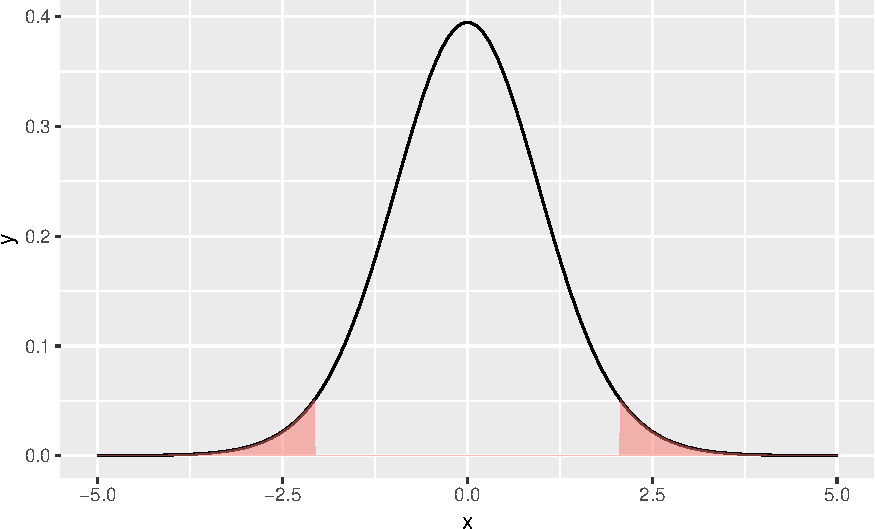
\includegraphics[width=0.7\linewidth]{regression-analysis_files/figure-latex/b0rjt-1} 

}

\caption{Rejection region for $\beta_0$}\label{fig:b0rjt}
\end{figure}

More importantly, we test \(\beta_1\) which means slope

\[H_0 : \beta_1 = \alpha_1 \qquad \text{vs} \qquad H_1 : \beta_1 \neq \alpha_1\]

\begin{equation}
  T = \frac{\hat\beta_1 - \alpha_1}{\hat\sigma \sqrt{\frac{1}{S_{xx}}}} \stackrel{H_0}{\sim} t(n - 2)
  \label{eq:b1test}
\end{equation}

For this test statistic \eqref{eq:b1test},

\[\text{reject}\: H_0 \quad \text{if} \: \lvert T \rvert > t_{\frac{\alpha}{2}}(n - 2)\]

Looking at these two statistics, we can intuitively know the meaning. As \(\lvert \hat\beta_1 - \alpha_1 \rvert\) becomes larger, the data support \(H_1\).

\hypertarget{analysis-of-variance}{%
\section{Analysis of Variance}\label{analysis-of-variance}}

\hypertarget{useful-distributions}{%
\subsection{Useful distributions}\label{useful-distributions}}

In linear regression setting, we usually assume \(\epsilon_i \stackrel{iid}{\sim}N(0, \sigma^2)\). There are some useful distributions around Normal.

\BeginKnitrBlock{proposition}[$\chi^2$-distribution]
\protect\hypertarget{prp:chisq}{}{\label{prp:chisq} \iffalse (\(\chi^2\)-distribution) \fi{} }Square of standard normal follows \(\chi^2\)-distribution.

If \(Z \sim N(0, 1)\), then \(Z^2 \sim \chi^2(1)\)

If \(Z_i \stackrel{indep}{\sim}N(0, 1)\), then \(Z_1^2 + \cdots + Z_n^2 \sim \chi^2(n)\)
\EndKnitrBlock{proposition}

\BeginKnitrBlock{proposition}[t-distribution]
\protect\hypertarget{prp:tdist}{}{\label{prp:tdist} \iffalse (t-distribution) \fi{} }Let \(Z \sim N(0, 1) \perp\!\!\!\perp V \sim \chi^2(m)\). Then

\[T = \frac{Z}{\sqrt{V / m}} \sim t(m)\]
\EndKnitrBlock{proposition}

\BeginKnitrBlock{proposition}[F-distribution]
\protect\hypertarget{prp:fdist}{}{\label{prp:fdist} \iffalse (F-distribution) \fi{} }Let \(V \sim \chi^2(m) \perp\!\!\!\perp W \sim \chi^2(n)\). Then

\[F = \frac{V / m}{W / n} \sim F(m, n)\]
\EndKnitrBlock{proposition}

Also, there is \emph{non-central analogue} of these three distributions, i.e.~starting from \(Z \sim N(\mu, 1)\).

\BeginKnitrBlock{proposition}[Noncentral $\chi^2$-distribution]
\protect\hypertarget{prp:nonchi}{}{\label{prp:nonchi} \iffalse (Noncentral \(\chi^2\)-distribution) \fi{} }Square of scaled normal follows non-central \(\chi^2\)-distribution.

If \(Z_i \stackrel{indep}{\sim}N(\mu_i, 1)\), then \(Z_1^2 + \cdots + Z_n^2 \sim \chi^2(n, \sum\limits_{i = 1}^n \mu_i^2)\)

\(\sum\limits_{i = 1}^n \mu_i^2\) is called a non-central parameter.
\EndKnitrBlock{proposition}

\BeginKnitrBlock{proposition}[Noncentral t-distribution]
\protect\hypertarget{prp:nontdist}{}{\label{prp:nontdist} \iffalse (Noncentral t-distribution) \fi{} }Let \(X \sim N(\mu, 1) \perp\!\!\!\perp V \sim \chi^2(m)\). Then

\[T = \frac{Z}{\sqrt{V / m}} \sim t(m, \mu)\]

\(\mu\) is called a non-central parameter.
\EndKnitrBlock{proposition}

\BeginKnitrBlock{proposition}[Noncentral F-distribution]
\protect\hypertarget{prp:nonfdist}{}{\label{prp:nonfdist} \iffalse (Noncentral F-distribution) \fi{} }Let \(V \sim \chi^2(m, \delta) \perp\!\!\!\perp W \sim \chi^2(n)\). Then

\[F = \frac{V / m}{W / n} \sim F(m, n, \delta)\]

\(\delta\) is called a non-central parameter.
\EndKnitrBlock{proposition}

\hypertarget{quadratic-form}{%
\subsection{Quadratic form}\label{quadratic-form}}

Now we can determine the distributions of various quadratic forms. The reason we are taking care of this is ANOVA deals with sum of squares, i.e.~quadratic form. See Corollary \ref{cor:projss} for this.

\begin{itemize}
\tightlist
\item
  \(SST = \mathbf{Y}^T(I - \Pi_{\mathbf{1}})\mathbf{Y}\)
\item
  \(SSR = \mathbf{Y}^T(\Pi_X - \Pi_{\mathbf{1}})\mathbf{Y}\)
\item
  \(SSE = \mathbf{Y}^T(I - \Pi_X)\mathbf{Y}\)
\end{itemize}

\BeginKnitrBlock{theorem}[Idempotent and symmetric]
\protect\hypertarget{thm:idem}{}{\label{thm:idem} \iffalse (Idempotent and symmetric) \fi{} }Let \(A \in \mathbb{R}^{k \times k}\) be idempotent and symmetric. Then

\begin{enumerate}[label=(\alph*)]
  \item $A^n$ is also idempotent \label{itm:idemone}
  \item $I - A$ is also idempotent \label{itm:idemtwo}
  \item Every eigenvalue of $A$ is either $0$ or $1$ so that $tr(A) = rank(A)$ \label{itm:idemthree}
\end{enumerate}
\EndKnitrBlock{theorem}

\BeginKnitrBlock{proof}
\iffalse{} {Proof. } \fi{}\(\ref{itm:idemone}\) and \(\ref{itm:idemtwo}\) are trivial.

\[(A^n)^2 = (A^2)^n = A^n\]

\[(I - A)^2 = I - 2A + A^2 = I - A\]

\(\ref{itm:idemthree}\)

Fix \(\lambda\) an eigenvalue of \(A\). Let \(\mathbf{v} \neq \mathbf{0}\) be the corresponding eigenvector.

By definition,

\[A\mathbf{v} = \lambda \mathbf{v}\]

Then

\[A^2\mathbf{v} = \lambda(A\mathbf{v}) = \lambda^2\mathbf{v}\]

and so \(\lambda^2\) is eigenvalue of \(A^2\).

Since \(A^2 = A\),

\[\lambda = \lambda^2\]

Hence,

\[\lambda = 0 \:\text{or}\: 1\]

Note that for every matrix and its eigenvalues \(\lambda_j\)

\[tr(A) = \sum_{j = 1}^p \lambda_j, \quad rank(A) = \text{the number of non-zero}\: \lambda_j\]

Since \(\lambda = 0, 1\) of A,

\[tr(A) = rank(A)\]
\EndKnitrBlock{proof}

\BeginKnitrBlock{proposition}[Independence]
\protect\hypertarget{prp:quadmvn}{}{\label{prp:quadmvn} \iffalse (Independence) \fi{} }Assume \(\mathbf{Y} \sim MVN(\mathbf\mu, \Sigma)\). Then

\begin{enumerate}[label=(\roman*)]
  \item If $A$ and $B$ are symmetric, $$Y^T AY \perp\!\!\!\perp Y^T BY \Leftrightarrow A\Sigma B = 0$$
  \item If $A$ is symmetric, $$Y^T AY \perp\!\!\!\perp BY \Leftrightarrow B\Sigma A = 0$$
\end{enumerate}
\EndKnitrBlock{proposition}

\BeginKnitrBlock{theorem}[Distribution of quadratic form]
\protect\hypertarget{thm:quaddist}{}{\label{thm:quaddist} \iffalse (Distribution of quadratic form) \fi{} }Assume that \(\mathbf{Y} \sim MVN(\mathbf\mu, I)\) and that \(A\) is symmetric and idempotent. Then

\[Y^T AY \sim \chi^2(K, \delta)\]

where \(K = rank(A)\) and \(\delta = \boldsymbol\mu^T A \boldsymbol\mu\). Furthermore,

\[
\begin{cases}
  E(Y^T AY) = K + \delta \\
  Var(Y^T AY) = 2(K + 2\delta)
\end{cases}
\]
\EndKnitrBlock{theorem}

\BeginKnitrBlock{corollary}[Inner product of standard normal vector]
\protect\hypertarget{cor:mvnchi}{}{\label{cor:mvnchi} \iffalse (Inner product of standard normal vector) \fi{} }Let \(\mathbf{Z} = (Z_1, \ldots, Z_n)^T \sim MVN(\mathbf{0}, I_n)\). Then

\[\mathbf{Z}^T\mathbf{Z} = \sum_{i = 1}^n Z_i^2 \sim \chi^2(n)\]
\EndKnitrBlock{corollary}

\BeginKnitrBlock{proof}
\iffalse{} {Proof. } \fi{}From Theorem \ref{thm:quaddist} point of view,

\[\mathbf{Z}^T\mathbf{Z} = \mathbf{Z}^T I_n \mathbf{Z}\]

Thus,

\[K = rank(I_n) = n\]

\[\delta = \mathbf{0}\]
\EndKnitrBlock{proof}

Using the above facts, we can now show distributions of sums of squares. First recall that

\[\mathbf{Y} \sim MVN(X\boldsymbol\beta, \sigma^2 I)\]

\BeginKnitrBlock{proposition}[Distribution of SSE]
\protect\hypertarget{prp:ssedist}{}{\label{prp:ssedist} \iffalse (Distribution of SSE) \fi{} }\[\frac{SSE}{\sigma^2} \sim \chi^2(n - 2, 0)\]
\EndKnitrBlock{proposition}

\BeginKnitrBlock{proof}
\iffalse{} {Proof. } \fi{}From Corollary \ref{cor:projss}, write

\[\frac{SSE}{\sigma^2} = \bigg(\frac{\mathbf{Y}}{\sigma}\bigg)^T (I - \Pi_X) \bigg(\frac{\mathbf{Y}}{\sigma}\bigg)\]

Note that

\[\frac{\mathbf{Y}}{\sigma} \sim MVN(\frac{1}{\sigma}X\boldsymbol\beta, I)\]

Since \(I - \Pi_X\) is idempotent and symmetric,

\[K = rank(I - \Pi_X) = tr(I - \Pi_X) = n - rank(\Pi_X) = n - 2\]

\begin{equation} \label{eq:delta1}
  \begin{split}
    \delta & = \bigg(\frac{X\boldsymbol\beta}{\sigma}\bigg)^T (I - \Pi_X) \bigg(\frac{X\boldsymbol\beta}{\sigma}\bigg) \\
    & = \frac{\boldsymbol\beta^TX^TX\boldsymbol\beta}{\sigma^2} - \frac{(\boldsymbol\beta^TX^T)X(X^TX)^{-1}X^T(X\boldsymbol\beta)}{\sigma^2} \\
    & = \frac{\boldsymbol\beta^TX^TX\boldsymbol\beta}{\sigma^2} - \frac{\boldsymbol\beta^TX^TX\boldsymbol\beta}{\sigma^2} \\
    & = 0
  \end{split}
\end{equation}

Hence,

\[\frac{SSE}{\sigma^2} \sim \chi^2(n - 2, 0)\]
\EndKnitrBlock{proof}

In case of \(SSE\), it always follows \(\chi^2(n - 2)\) no matter what \(H_0\) is. However, \(SSR\) and \(SST\) depend on \(\beta_1\) that we want to test.

\BeginKnitrBlock{proposition}[Distribution of SSR]
\protect\hypertarget{prp:ssrdist}{}{\label{prp:ssrdist} \iffalse (Distribution of SSR) \fi{} }\[\frac{SSR}{\sigma^2} \sim \chi^2(1, \delta)\]

where \(\delta = \frac{1}{\sigma^2}\sum\limits_{i = 1}^n (x_i - \overline{x})^2 \beta_1^2 = \frac{S_{xx}\beta_1^2}{\sigma^2}\)
\EndKnitrBlock{proposition}

\BeginKnitrBlock{proof}
\iffalse{} {Proof. } \fi{}From Corollary \ref{cor:projss}, write

\[\frac{SSR}{\sigma^2} = \bigg(\frac{\mathbf{Y}}{\sigma}\bigg)^T (\Pi_X - \Pi_{\mathbf{1}}) \bigg(\frac{\mathbf{Y}}{\sigma}\bigg)\]

Note that \(\Pi_X - \Pi_{\mathbf{1}}\) is symmetric idempotent. One proceeds in a similar way.

\[K = rank(\Pi_X - \Pi_{\mathbf{1}}) = tr(\Pi_X - \Pi_{\mathbf{1}}) = rank(\Pi_X) - rank(\Pi_{\mathbf{1}}) = 2 - 1 = 1\]

\begin{equation*}
  \begin{split}
    \delta & = \bigg(\frac{X\boldsymbol\beta}{\sigma}\bigg)^T (\Pi_X - \Pi_{\mathbf{1}}) \bigg(\frac{X\boldsymbol\beta}{\sigma}\bigg) \qquad \because \frac{\mathbf{Y}}{\sigma} \sim MVN(\frac{1}{\sigma}X\boldsymbol\beta, I) \\
    & = \frac{\boldsymbol\beta^T \Big\{ X^T(\Pi_X - \Pi_{\mathbf{1}})X \Big\} \boldsymbol\beta }{\sigma^2}
  \end{split}
\end{equation*}

Since \(\mathbf{1} \in Col(X)\),

\[\Pi_X \mathbf{1} = \mathbf{1}\]

It gives that

\begin{equation} \label{eq:ssrquad1}
  \mathbf{1}^T(\Pi_X - \Pi_{\mathbf{1}})\mathbf{1} = 0
\end{equation}

If \(\mathbf{x} \neq \mathbf{1}\), then we have

\begin{equation} \label{eq:ssrquad2}
  \mathbf{x}^T(\Pi_X - \Pi_{\mathbf{1}})\mathbf{x} = \sum_{i = 1}^n (x_i - \overline{x})^2 = S_{xx}
\end{equation}

Recall that

\[\overline{x}\mathbf{1} = \mathbf{1}(\mathbf{1}^T\mathbf{1})^{-1}\mathbf{1}^T\mathbf{x} = \Pi_{\mathbf{1}}\mathbf{x}\]

Then we have

\begin{equation} \label{eq:ssrquad3}
  \mathbf{1}^T(\Pi_X - \Pi_{\mathbf{1}})\mathbf{x} = \sum x_i - n \overline{x} = 0
\end{equation}

By symmetry,

\begin{equation} \label{eq:ssrquad4}
  \mathbf{x}^T(\Pi_X - \Pi_{\mathbf{1}})\mathbf{1} = n \overline{x} - \sum x_i = 0
\end{equation}

Hence by partitioning \(X = [\mathbf{1} \mid \mathbf{x}]\),

\begin{equation} \label{eq:delta2}
  \begin{split}
    \delta & = \frac{\boldsymbol\beta^T \Big\{ [\mathbf{1} \mid \mathbf{x}]^T(\Pi_X - \Pi_{\mathbf{1}})[\mathbf{1} \mid \mathbf{x}] \Big\} \boldsymbol\beta }{\sigma^2} \\
    & = \frac{\boldsymbol\beta^T \begin{bmatrix} \eqref{eq:ssrquad1} & \eqref{eq:ssrquad3} \\ \eqref{eq:ssrquad4} & \eqref{eq:ssrquad2} \end{bmatrix} \boldsymbol\beta}{\sigma^2} \\
    & = \frac{\boldsymbol\beta^T \begin{bmatrix} 0 & 0 \\ 0 & S_{xx} \end{bmatrix} \boldsymbol\beta}{\sigma^2} \\
    & = \frac{S_{xx}\beta_1^2}{\sigma^2}
  \end{split}
\end{equation}
\EndKnitrBlock{proof}

\BeginKnitrBlock{proposition}[Independence]
\protect\hypertarget{prp:ssind}{}{\label{prp:ssind} \iffalse (Independence) \fi{} }SSE and SSR are independent, i.e.

\[SSE \perp\!\!\!\perp SSR\]
\EndKnitrBlock{proposition}

\BeginKnitrBlock{proof}
\iffalse{} {Proof. } \fi{}Note that both \(SSE\) and \(SSR\) are quadratic forms of \(\mathbf{Y} \sim MVN(X\boldsymbol\beta, \sigma^2 I)\) and that each \(I - \Pi_X\) and \(\Pi_X - \Pi_{\mathbf{1}}\) is symmetric. Then from Proposition \ref{prp:quadmvn},

Claim: \((I - \Pi_X)(\sigma^2I)(\Pi_X - \Pi_{\mathbf{1}}) = 0\), i.e.~\((I - \Pi_X)(\Pi_X - \Pi_{\mathbf{1}}) = 0\)

It is obvious that

\[\Pi_X\Pi_{\mathbf{1}} = \Pi_{\mathbf{1}}\]

Then

\begin{equation*}
  \begin{split}
    (I - \Pi_X)(\Pi_X - \Pi_{\mathbf{1}}) & = \Pi_X - \Pi_{\mathbf{1}} - \Pi_X^2 + \Pi_X\Pi_{\mathbf{1}} \\
    & = \Pi_X - \Pi_{\mathbf{1}} - \Pi_X + \Pi_{\mathbf{1}} \qquad \because \text{idempotent} \\
    & = 0
  \end{split}
\end{equation*}

This completes the proof.
\EndKnitrBlock{proof}

\BeginKnitrBlock{proposition}[Independence]
\protect\hypertarget{prp:ssbind}{}{\label{prp:ssbind} \iffalse (Independence) \fi{} }SSE and \((\hat\beta_0, \hat\beta_1)\) are independent, i.e.

\[SSE \perp\!\!\!\perp(\hat\beta_0, \hat\beta_1)^T\]
\EndKnitrBlock{proposition}

\BeginKnitrBlock{proof}
\iffalse{} {Proof. } \fi{}Note that

\[\boldsymbol{\hat\beta}= (\hat\beta_0, \hat\beta_1)^T = (X^TX)^{-1}X^T\mathbf{Y}\]

Since \(I - \Pi_X\) of \(SSE\) is symmetric, from Proposition \ref{prp:quadmvn},

Claim: \(((X^TX)^{-1}X^T)(\sigma^2I)(I - \Pi_X) = 0\), i.e.~\(((X^TX)^{-1}X^T)(I - \Pi_X) = 0\)

Since \(\Pi_X = X(X^TX)^{-1}X^T\),

\begin{equation*}
  \begin{split}
    ((X^TX)^{-1}X^T)(I - \Pi_X) & = (X^TX)^{-1}X^T - (X^TX)^{-1}X^TX(X^TX)^{-1}X^T \\
    & = (X^TX)^{-1}X^T - (X^TX)^{-1}X^T \\
    & = 0
  \end{split}
\end{equation*}

This completes the proof.
\EndKnitrBlock{proof}

\BeginKnitrBlock{proposition}[Distribution of SST]
\protect\hypertarget{prp:sstdist}{}{\label{prp:sstdist} \iffalse (Distribution of SST) \fi{} }\[\frac{SST}{\sigma^2} \sim \chi^2(n - 1, \delta)\]

where \(\delta = \sum\limits_{i = 1}^n (x_i - \overline{x})^2 \beta_1^2 = \frac{S_{xx}\beta_1^2}{\sigma^2}\)
\EndKnitrBlock{proposition}

\BeginKnitrBlock{proof}
\iffalse{} {Proof. } \fi{}It proceedes in a similary way from Corollary \ref{cor:projss}

\[\frac{SST}{\sigma^2} = \bigg(\frac{\mathbf{Y}}{\sigma}\bigg)^T (I - \Pi_{\mathbf{1}}) \bigg(\frac{\mathbf{Y}}{\sigma}\bigg)\]

Since \(I - \Pi_{\mathbf{1}}\) is symmetric idempotent,

\[K = rank(I - \Pi_{\mathbf{1}}) = tr(I - \Pi_{\mathbf{1}}) = n - rank(\Pi_{\mathbf{1}}) = n - 1\]

Since \(\mathbf{1} \in sp( \{ \mathbf{1} \})\),

\[\Pi_{\mathbf{1}} \mathbf{1} = \mathbf{1}\]

Hence,

\begin{equation*}
  \begin{split}
    \delta & = \bigg(\frac{X\boldsymbol\beta}{\sigma}\bigg)^T (I - \Pi_{\mathbf{1}}) \bigg(\frac{X\boldsymbol\beta}{\sigma}\bigg) \\
    & = \frac{S_{xx}\beta_1^2}{\sigma^2} \qquad \because \eqref{eq:delta1} \:\text{and}\: \eqref{eq:delta2} 
  \end{split}
\end{equation*}
\EndKnitrBlock{proof}

\hypertarget{anova-for-testing-significance-of-regression}{%
\subsection{ANOVA for testing significance of regression}\label{anova-for-testing-significance-of-regression}}

Recall that

\[SST = SSR + SSE\]

\begin{itemize}
\tightlist
\item
  \(SST\): the variation of a response itself
\item
  \(SSR\): the variation of a response \emph{explained by the model}
\item
  \(SSE\): the variation of a response that \emph{cannot be explained by the model}
\end{itemize}

As mentioned in section \ref{decompsst}, whether the model is useful or not can depend on the proportion of \(SSR\) versus \(SSE\) in constant \(SST\). When \(SSR\) is large compared to \(SSE\), we can say that the model is good. On the other hand, when \(SSR\) is not large, the model might be poor. This is what \(R^2\) measures intuitively.

However, this direct comparison somtimes does not work in many times. Both \(SSR\) and \(SSE\) comes from different distribution, which have different degrees of freedom. So we \emph{compare standardized versions}, i.e.~divided by the degrees of freedom.

\BeginKnitrBlock{definition}[Degrees of freedom]
\protect\hypertarget{def:dof}{}{\label{def:dof} \iffalse (Degrees of freedom) \fi{} }Degrees of freedom of each sum of squares is

\[df = \text{the number of deviation} - \text{the number of linear constraints}\]
\EndKnitrBlock{definition}

\BeginKnitrBlock{corollary}[df of SS]
\protect\hypertarget{cor:dfss}{}{\label{cor:dfss} \iffalse (df of SS) \fi{} }\(df\) of each sum of square is computed as

\begin{enumerate}[label=(\alph*)]
  \item $df(SST) = n - 1$ \label{itm:dfssone}
  \item $df(SSR) = 1$ \label{itm:dfsstwo}
  \item $df(SSE) = n - 2$ \label{itm:dfssthree}
\end{enumerate}
\EndKnitrBlock{corollary}

\BeginKnitrBlock{proof}
\iffalse{} {Proof. } \fi{}\(\ref{itm:dfssone}\)

Since \(\sum (Y_i - \overline{Y}) = 0\), we have \(1\) linear constraints. Thus,

\[df(SST) = n - 1\]

\(\ref{itm:dfsstwo}\)

Note that \(\hat{Y_i} - \overline{Y} = \hat\beta_1(x_i - \overline{x})\)

where \(\sum (x_i - \overline{x}) = 0\).

Thus,

\[df(SSR) = n - (n - 1) = 1\]

\(\ref{itm:dfssthree}\)

From Example \ref{exm:usingnormal}, \(\sum (Y_i - \hat{Y_i}) = 0\) and \(\sum x_i (Y_i - \hat{Y_i}) = 0\).

Thus,

\[df(SSE) = n - 2\]
\EndKnitrBlock{proof}

Dividing sum of squares in \(df\), we can standardize it.

\BeginKnitrBlock{definition}[Mean square]
\protect\hypertarget{def:ms}{}{\label{def:ms} \iffalse (Mean square) \fi{} }Mean square is a sum of square \(SS\) divided by its degree of freedom \(df\)

\[MS := \frac{SS}{df}\]
\EndKnitrBlock{definition}

Using the values of corollary \ref{cor:dfss} we can define each mean square for \(SSR\) and \(SSE\).

\BeginKnitrBlock{definition}[Regression mean square]
\protect\hypertarget{def:msr}{}{\label{def:msr} \iffalse (Regression mean square) \fi{} }\[MSR := \frac{SSR}{1} = SSR\]
\EndKnitrBlock{definition}

From Proposition \ref{prp:ssrdist}, the following corollary can be drawn.

\BeginKnitrBlock{corollary}[Distribution of MSR]
\protect\hypertarget{cor:msrdist}{}{\label{cor:msrdist} \iffalse (Distribution of MSR) \fi{} }Under \(H_0: \beta_1 = 0\),

\[\frac{SSR}{\sigma^2} \stackrel{H_0}{\sim} \chi^2(1)\]
\EndKnitrBlock{corollary}

Now standardize residual sum of square.

\BeginKnitrBlock{definition}[Residual mean square]
\protect\hypertarget{def:mse}{}{\label{def:mse} \iffalse (Residual mean square) \fi{} }\[MSE := \frac{SSE}{n - 2}\]
\EndKnitrBlock{definition}

From Proposition \ref{prp:ssrdist}, we can construct same statistic. In fact, \(\frac{SSE}{\sigma^2}\) follows \(\chi^2(n - 2)\) whether or not \(\beta_1\) is zero. Its \(\delta = 0\).

\BeginKnitrBlock{corollary}[Distribution of MSE]
\protect\hypertarget{cor:msedist}{}{\label{cor:msedist} \iffalse (Distribution of MSE) \fi{} }\[\frac{SSE}{\sigma^2} \sim \chi^2(n - 2)\]
\EndKnitrBlock{corollary}

Finally, we can now use Proposition \ref{prp:fdist} so that

\[
F \equiv \frac{MSR}{MSE} = \frac{\frac{SSE / \sigma^2 \sim \chi^2(1)}{1}}{\frac{SSR / \sigma^2 \stackrel{H_0}{\sim}\chi^2(n - 2)}{n - 2}} \stackrel{H_0}{\sim}F(1, n - 2)
\]

By construction, this test statistic is used for

\[H_0: \beta_1 = 0\]

which means that the predictor does not explain the response anything. In other words, we are testing that

\begin{equation}
  H_0: \text{Model is not useful at all} \qquad \text{vs} \qquad H_1: \text{Model can explain data}
  \label{eq:goodfit}
\end{equation}

\BeginKnitrBlock{remark}[F statistic on testing significance]
\iffalse{} {Remark (F statistic on testing significance). } \fi{}Null hypothesis \eqref{eq:goodfit} can be tested with \(F\)-statistic.

\[F_0 = \frac{MSR}{MSE} = \frac{SSR / df(SSR)}{SSE / df(SSE)} \stackrel{H_0}{\sim}F(df(SSR), df(SSE))\]
\EndKnitrBlock{remark}

Here, it is

\[F_0 = \frac{SSR / 1}{SSE / (n - 2)}\]

Then we reject \(H_0\) if

\[F_0 > F_\alpha\bigg( df(SSR), df(SSE) \bigg)\]

\begin{figure}[H]

{\centering 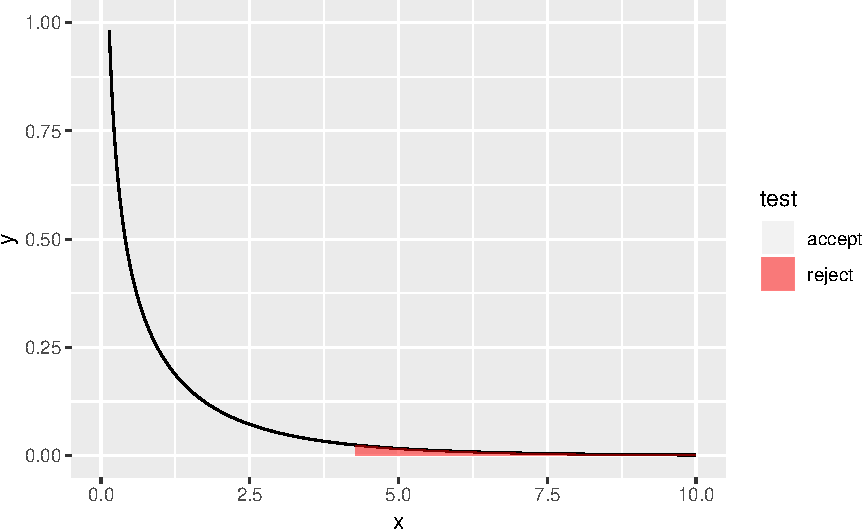
\includegraphics[width=0.7\linewidth]{regression-analysis_files/figure-latex/goodfitfig-1} 

}

\caption{Rejection region for significance testing}\label{fig:goodfitfig}
\end{figure}

\begin{Shaded}
\begin{Highlighting}[]
\KeywordTok{summary}\NormalTok{(delv_fit)}
\CommentTok{#> }
\CommentTok{#> Call:}
\CommentTok{#> lm(formula = y ~ x, data = delv)}
\CommentTok{#> }
\CommentTok{#> Residuals:}
\CommentTok{#>    Min     1Q Median     3Q    Max }
\CommentTok{#> -7.581 -1.874 -0.349  2.181 10.634 }
\CommentTok{#> }
\CommentTok{#> Coefficients:}
\CommentTok{#>             Estimate Std. Error t value Pr(>|t|)    }
\CommentTok{#> (Intercept)    3.321      1.371    2.42    0.024 *  }
\CommentTok{#> x              2.176      0.124   17.55  8.2e-15 ***}
\CommentTok{#> ---}
\CommentTok{#> Signif. codes:  0 '***' 0.001 '**' 0.01 '*' 0.05 '.' 0.1 ' ' 1}
\CommentTok{#> }
\CommentTok{#> Residual standard error: 4.18 on 23 degrees of freedom}
\CommentTok{#> Multiple R-squared:  0.93,   Adjusted R-squared:  0.927 }
\CommentTok{#> F-statistic:  308 on 1 and 23 DF,  p-value: 8.22e-15}
\end{Highlighting}
\end{Shaded}

This statistic is \texttt{F-statistic} included in \texttt{summary.lm()} output. This is saved as \texttt{\$fstatistic}.

\begin{Shaded}
\begin{Highlighting}[]
\KeywordTok{summary}\NormalTok{(delv_fit)}\OperatorTok{$}\NormalTok{fstatistic}
\CommentTok{#> value numdf dendf }
\CommentTok{#>   308     1    23}
\end{Highlighting}
\end{Shaded}

We usually summarize these statistic in table form, so called \emph{ANOVA table}.

\begin{longtable}[]{@{}cccccc@{}}
\toprule
Source & SS & df & MS & F & p-value\tabularnewline
\midrule
\endhead
Model & \(SSR\) & \(1\) & \(MSR\) & \(F_0\) & p-value\tabularnewline
Error & \(SSE\) & \(n - 2\) & \(MSE\) & &\tabularnewline
Total & \(SST\) & \(n - 1\) & & &\tabularnewline
\bottomrule
\end{longtable}

To get this table, just use \texttt{anova()} for \texttt{lm} object.

\begin{Shaded}
\begin{Highlighting}[]
\KeywordTok{anova}\NormalTok{(delv_fit)}
\CommentTok{#> Analysis of Variance Table}
\CommentTok{#> }
\CommentTok{#> Response: y}
\CommentTok{#>           Df Sum Sq Mean Sq F value  Pr(>F)    }
\CommentTok{#> x          1   5382    5382     308 8.2e-15 ***}
\CommentTok{#> Residuals 23    402      17                    }
\CommentTok{#> ---}
\CommentTok{#> Signif. codes:  0 '***' 0.001 '**' 0.01 '*' 0.05 '.' 0.1 ' ' 1}
\end{Highlighting}
\end{Shaded}

Since the last \texttt{Total} row is just sum of the model and error, the function does not give it. To use this table as \texttt{data.frame} more easily, just implement \texttt{broom::tidy} as before.

\begin{Shaded}
\begin{Highlighting}[]
\KeywordTok{anova}\NormalTok{(delv_fit) }\OperatorTok\StringTok{ }
\StringTok{  }\NormalTok{broom}\OperatorTok{::}\KeywordTok{tidy}\NormalTok{()}
\CommentTok{#> # A tibble: 2 x 6}
\CommentTok{#>   term         df sumsq meansq statistic   p.value}
\CommentTok{#>   <chr>     <int> <dbl>  <dbl>     <dbl>     <dbl>}
\CommentTok{#> 1 x             1 5382. 5382.       308.  8.22e-15}
\CommentTok{#> 2 Residuals    23  402.   17.5       NA  NA}
\end{Highlighting}
\end{Shaded}

Denote that here \emph{simple linear regression setting} \(F\)-statistic and \(t\)-statistic of Equation \eqref{eq:b1test} perform exactly same thing, \(H_0 : \beta_1 = 0\). In fact, we know that

\[F(1, k) \stackrel{d}{=} T_k^2\]

\BeginKnitrBlock{remark}
\iffalse{} {Remark. } \fi{}In the simple linear regression setting, \(F\)-test for significance and \(t\)-test for no slope are equivalent, i.e.~under \(H_0 : \beta_1 = 0\)

\[F_0 = \frac{\hat\beta_1 S_{xx}}{\hat\sigma^2} = \bigg( \frac{\hat\beta_1}{\hat\sigma / \sqrt{S_{xx}}} \bigg) = T_0^2\]
\EndKnitrBlock{remark}

\hypertarget{multiple}{%
\chapter{Multiple Linear Regression}\label{multiple}}

\hypertarget{model-1}{%
\section{Model}\label{model-1}}

\begin{Shaded}
\begin{Highlighting}[]
\NormalTok{(cem <-}\StringTok{ }\NormalTok{MPV}\OperatorTok{::}\NormalTok{cement }\OperatorTok\StringTok{ }\KeywordTok{tbl_df}\NormalTok{())}
\CommentTok{#> # A tibble: 13 x 5}
\CommentTok{#>       y    x1    x2    x3    x4}
\CommentTok{#>   <dbl> <dbl> <dbl> <dbl> <dbl>}
\CommentTok{#> 1  78.5     7    26     6    60}
\CommentTok{#> 2  74.3     1    29    15    52}
\CommentTok{#> 3 104.     11    56     8    20}
\CommentTok{#> 4  87.6    11    31     8    47}
\CommentTok{#> 5  95.9     7    52     6    33}
\CommentTok{#> 6 109.     11    55     9    22}
\CommentTok{#> # ... with 7 more rows}
\end{Highlighting}
\end{Shaded}

Above is a data set about cement and concerning four ingredients from the \citet{Montgomery:2015aa} textbook.

\begin{itemize}
\tightlist
\item
  \texttt{y}: heat evolved in calories per gram of cement
\item
  \texttt{x1}: tricalcium aluminate
\item
  \texttt{x2}: tricalcium silicate
\item
  \texttt{x3}: tetracalcium alumino ferrite
\item
  \texttt{x4}: dicalcium silicate
\end{itemize}

Given data \((x_{11}, x_{12}, \ldots, x_{1p}, Y_1), \ldots, (x_{n1}, x_{n2}, \ldots, x_{np}, Y_n)\) (\(p = 4\)), we try to fit linear regression model

\[Y_i = \beta_0 + \beta_1 x_{i1} + \cdots + \beta_p x_{ip} + \epsilon_{i}\]

with

\[\epsilon_i \stackrel{iid}{\sim}(0, \sigma^2)\]

Compared to simple linear regression problem \ref{simple}, we have more parameters for coefficients

\[(\beta_0, \beta_1, \ldots, \beta_p, \sigma^2)\]

Each \(\beta_j\) is a change of \(Y\) when each predictor variable \(x_j\) increases in 1 unit while the others fixed. In this part, we use \emph{matrix notation}. Extending our former matrix work \ref{matnot},

\[
\underset{\huge \mathbf{Y}}{\begin{bmatrix}
  Y_1 \\
  Y_2 \\
  \vdots \\
  Y_n
\end{bmatrix}} = \underset{\huge X}{\begin{bmatrix}
  1 & x_{11} & \cdots & x_{1p} \\
  1 & x_{21} & \cdots & x_{2p} \\
  \vdots & \vdots & \vdots & \vdots \\
  1 & x_{n1} & \cdots & x_{np}
\end{bmatrix}} \underset{\huge \boldsymbol\beta}{\begin{bmatrix}
  \beta_0 \\
  \vdots \\
  \beta_p
\end{bmatrix}} + \underset{\huge \E}{\begin{bmatrix}
  \epsilon_1 \\
  \epsilon_2 \\
  \vdots \\
  \epsilon_n
\end{bmatrix}}
\]

where \(\epsilon_i\) are i.i.d., and

\[E \E = \mathbf{0}\]

\[Var \E = \sigma^2 I\]

\hypertarget{least-square-estimation}{%
\section{Least Square Estimation}\label{least-square-estimation}}

Write \(\boldsymbol\beta \equiv (\beta_1, \ldots, \beta_p)^T \in \mathbb{R}^{p + 1}\). Extend Equation \eqref{eq:qmatrix}.

\begin{equation}
  \begin{split}
    \boldsymbol{\hat\beta}& = \argmin_{ \boldsymbol\beta\in \mathbb{R}^{p + 1}} \sum_{i = 1}^n (Y_i - \beta_0 - \beta_1 x_{i1} - \cdots - \beta_p x_{ip})^2 \\
    & = \argmin_{ \boldsymbol\beta\in \mathbb{R}^{p + 1}} \lVert \mathbf{Y} - \beta_0 \mathbf{1} - \beta_1 \mathbf{x}_1 - \cdots - \beta_p \mathbf{x}_p \rVert^2 \\
    & = \argmin_{ \boldsymbol\beta\in \mathbb{R}^{p + 1}} \lVert \mathbf{Y} - X \boldsymbol\beta\rVert^2
  \end{split}
  \label{eq:qmultiple}
\end{equation}

As discussed, the solution \(\boldsymbol{\hat\beta}\) is related to the projection. \(X\boldsymbol{\hat\beta}\) is a projection of \(\mathbf{Y}\) onto \(Col(X)\).

\hypertarget{normal-equation}{%
\subsection{Normal equation}\label{normal-equation}}

Now recap the section \ref{solproj}. Fundamental subspaces theorem \ref{thm:fundsub} implies that

\[\mathbf{Y} - X \boldsymbol{\hat\beta}\in Col(X)^{\perp} = N(X^T)\]

From the second part of subset, i.e.~\(N(X^T)\), we now have \emph{Normal equation}

\begin{equation}
  X^T(\mathbf{Y} - X \boldsymbol{\hat\beta}) = \mathbf{0}
  \label{eq:multeq}
\end{equation}

This is equivalent to

\[X^T\mathbf{Y} = X^TX \boldsymbol{\hat\beta}\]

Hence, if \(X^T X\) is invertible, the equation gives unique solution

\[\boldsymbol{\hat\beta}= (X^TX)^{-1}X^T \mathbf{Y}\]

Our first question is when \(X^T X\) is invertible, and Theorem \ref{thm:fullrank} have said that it is when the model matrix \(X\) is full rank.

\BeginKnitrBlock{lemma}
\protect\hypertarget{lem:modelnnd}{}{\label{lem:modelnnd} }Let \(X \in \mathbb{R}^{n \times (p + 1)}\) be any model matrix. Then \(X^T X\) is always non-negative definite.

\[\forall \mathbf{v} \in \mathbb{R}^{p + 1} : \mathbf{v}^T(X^T X)\mathbf{v} \ge 0\]
\EndKnitrBlock{lemma}

\BeginKnitrBlock{proof}
\iffalse{} {Proof. } \fi{}Let \(\mathbf{v} \in \mathbb{R}^{p + 1}\). Then

\[\mathbf{v}^T(X^T X)\mathbf{v} = (X\mathbf{v})^T (X\mathbf{v}) = \lVert X\mathbf{v} \rVert^2 \ge 0\]
\EndKnitrBlock{proof}

This lemma can also prove our Theorem \ref{thm:fullrank}.

\BeginKnitrBlock{theorem}
\protect\hypertarget{thm:fullrank2}{}{\label{thm:fullrank2} }Let \(\mathbf{Y} = X\boldsymbol\beta\) inconsistent and let \(X \in \mathbb{R}^{n \times (p + 1)}\) with \(n > p + 1\).

If \(rank(X) = p + 1\), i.e.~full rank, then \(X^T X\) is invertible.
\EndKnitrBlock{theorem}

\BeginKnitrBlock{proof}
\iffalse{} {Proof. } \fi{}Let \(\mathbf{c} \in \mathbb{R}^{(p + 1)}\)

Suppose that \(X^T X\) is positive definite.

\begin{equation*}
  \begin{split}
    & \Leftrightarrow \mathbf{c}^TX^T X \mathbf{c} = 0 \quad \text{implies} \quad \mathbf{c} = \mathbf{0} \\
    & \Leftrightarrow X\mathbf{c} = \mathbf{0} \quad \text{implies} \quad \mathbf{c} = \mathbf{0} \\
    & \Leftrightarrow \text{columns of}\: X \:\text{linearly independent} \\
    & \Leftrightarrow rank(X) = p + 1
  \end{split}
\end{equation*}
\EndKnitrBlock{proof}

\hypertarget{orthogonal-decomposition}{%
\subsection{Orthogonal decomposition}\label{orthogonal-decomposition}}

\BeginKnitrBlock{theorem}
\protect\hypertarget{thm:orthonormal}{}{\label{thm:orthonormal} }Let \(Col(X)\) be a subspace of \(\mathbb{R}^n\), let \(\mathbf{Y} \in \mathbb{R}^n\), and let \(\{ \mathbf{u}_0, \ldots, \mathbf{u}_{p} \}\) be an orthonormal basis for \(Col(X)\). If

\[\mathbf{\hat{Y}} = \sum_{j = 0}^p \hat\beta_j \mathbf{u}_j\]

where

\[\hat\beta_j = \Pi(\mathbf{Y} \mid R(\mathbf{u}_j)) \quad \text{for each} \: i\]

then \(\mathbf{\hat{Y}} - \mathbf{Y} \in Col(X)^{\perp}\).
\EndKnitrBlock{theorem}

\BeginKnitrBlock{theorem}
\protect\hypertarget{thm:orthonormalproj}{}{\label{thm:orthonormalproj} }Under the hypothesis of Theorem \ref{thm:orthonormal}, \(\mathbf{\hat{Y}} \in Col(X)\) is the closest to \(\mathbf{Y}\) amongst its any element \(\mathbf{p}\), i.e.

\[\Vert \mathbf{p} - \mathbf{Y} \Vert > \Vert \mathbf{\hat{Y}} - \mathbf{Y} \Vert\]

for any \(\mathbf{p} \neq \mathbf{\hat{Y}}\) in \(Col(X)\)
\EndKnitrBlock{theorem}

In other words, projection of \(\mathbf{Y}\) onto \(Col(X)\), \(\mathbf{\hat{Y}}\) can be \emph{represented as sum of projections of} \(\mathbf{Y}\) \emph{onto each (orthogonal) individual variable}. Before looking at individual basis, consider two-block space.

Write

\[
X = \left[\begin{array}{c|ccc}
  1 & x_{11} & \cdots & x_{1p} \\
  1 & x_{21} & \cdots & x_{2p} \\
  \vdots & \vdots & \vdots & \vdots \\
  1 & x_{n1} & \cdots & x_{np}
\end{array}\right] = [\mathbf{1}, \mathbb{X}_A]
\]

Consider \(R(X)\), \(R(\mathbf{1})\), and \(R(\mathbb{X}_A)\).

To decompose subspace \(R(X)\), we try to orthogonalize \(\mathbf{1}\) and \(\mathbb{X}_A\). By Theorem \ref{thm:orthonormal}, we have

\[\mathbf{1} \perp \mathbb{X}_A - \Pi_{\mathbf{1}}\mathbb{X}_A\]

In fact, the right one \(\mathbb{X}_A - \Pi_{\mathbf{1}}\mathbb{X}_A\) is the \emph{residual after simple linear regression} \(\mathbb{X}_A\) onto \(\mathbf{1}\). We have seen in Figure \ref{fig:simpledraw2} of section \ref{matnot} that the \emph{residual is orthogonal to predictor vector}. In this procedure, we choose residual as new predictor instead of response in simple linear regression, i.e.~\(\mathbb{X}_A\). If this is done to individual predictor variables, it is called \emph{successive orthogonalization} and it will be coved next section with QR decomposition.

Theorem \ref{thm:dsum} implies that

\[R(X) = R(\mathbf{1}) \oplus R(\mathbb{X}_A - \Pi_{\mathbf{1}}\mathbb{X}_A)\]

\BeginKnitrBlock{theorem}[Orthogonal decomposition]
\protect\hypertarget{thm:orthdecomp}{}{\label{thm:orthdecomp} \iffalse (Orthogonal decomposition) \fi{} }Let \(X = [\mathbf{1}, \mathbb{X}_A]\). Then

\begin{enumerate}[label=(\roman*)]
  \item $$R(X) = R(\mathbf{1}) \oplus R(\mathbb{X}_A - \Pi_{\mathbf{1}}\mathbb{X}_A)$$ \label{itm:orthdecompone}
  \item $$\Pi(\cdot \mid R(X)) = \Pi(\cdot \mid R(\mathbf{1})) + \Pi(\cdot \mid R(\mathbb{X}_A - \Pi_{\mathbf{1}}\mathbb{X}_A))$$ \label{itm:orthdecomptwo}
\end{enumerate}
\EndKnitrBlock{theorem}

Write

\[\mathbb{X}_{A, \perp} := \mathbb{X}_A - \Pi_{\mathbf{1}}\mathbb{X}_A\]

Note that

\[\Pi_{\mathbf{1}} = \mathbf{1}(\mathbf{1}^T\mathbf{1})^{-1}\mathbf{1}^T = \frac{1}{n}\mathbf{1}\mathbf{1}^T\]

Then

\begin{equation}
  \begin{split}
    X\boldsymbol{\hat\beta} & = \hat\beta_0\mathbf{1} + \mathbb{X}_A\boldsymbol{\hat\beta}_A \\
    & = \hat\beta_0\mathbf{1} + (\mathbb{X}_{A, \perp} + \Pi_{\mathbf{1}}\mathbb{X}_A)\boldsymbol{\hat\beta}_A \\
    & = \Big(\hat\beta_0 + \frac{1}{n}\mathbf{1}^T\mathbb{X}_A\boldsymbol{\hat\beta}_A \Big)\mathbf{1} + \mathbb{X}_{A,\perp}\boldsymbol{\hat\beta}_A \qquad \because \hat\beta_0 + \frac{1}{n}\mathbf{1}^T\mathbb{X}_A\boldsymbol{\hat\beta}_A \in \mathbb{R}
  \end{split}
  \label{eq:blockfit}
\end{equation}

From (ii) of Theorem \ref{thm:orthdecomp},

\begin{equation}
  \begin{split}
    \Pi(\mathbf{Y} \mid R(X)) & = \Pi(\mathbf{Y} \mid R(\mathbf{1})) + \Pi(\mathbf{Y} \mid R(\mathbb{X}_{A,\perp})) \\
    & = \overline{Y}\mathbf{1} + \mathbb{X}_{A,\perp}(\mathbb{X}_{A,\perp}^T\mathbb{X}_{A,\perp})^{-1}\mathbb{X}_{A,\perp}^T\mathbf{Y}
  \end{split}
  \label{eq:decompfit}
\end{equation}

Since \(\mathbf{1} \perp \mathbb{X}_{A, \perp}\), Equations \eqref{eq:blockfit} and \eqref{eq:decompfit} imply that

\begin{equation}
  \begin{cases}
    \hat\beta_0 = \overline{Y} - \frac{1}{n}\mathbf{1}^T\mathbb{X}_A\boldsymbol{\hat\beta}_A \\
    \boldsymbol{\hat\beta}_A = (\mathbb{X}_{A,\perp}^T\mathbb{X}_{A,\perp})^{-1}\mathbb{X}_{A,\perp}^T\mathbf{Y}
  \end{cases}
  \label{eq:orthbeta}
\end{equation}

\begin{figure}[H]

{\centering 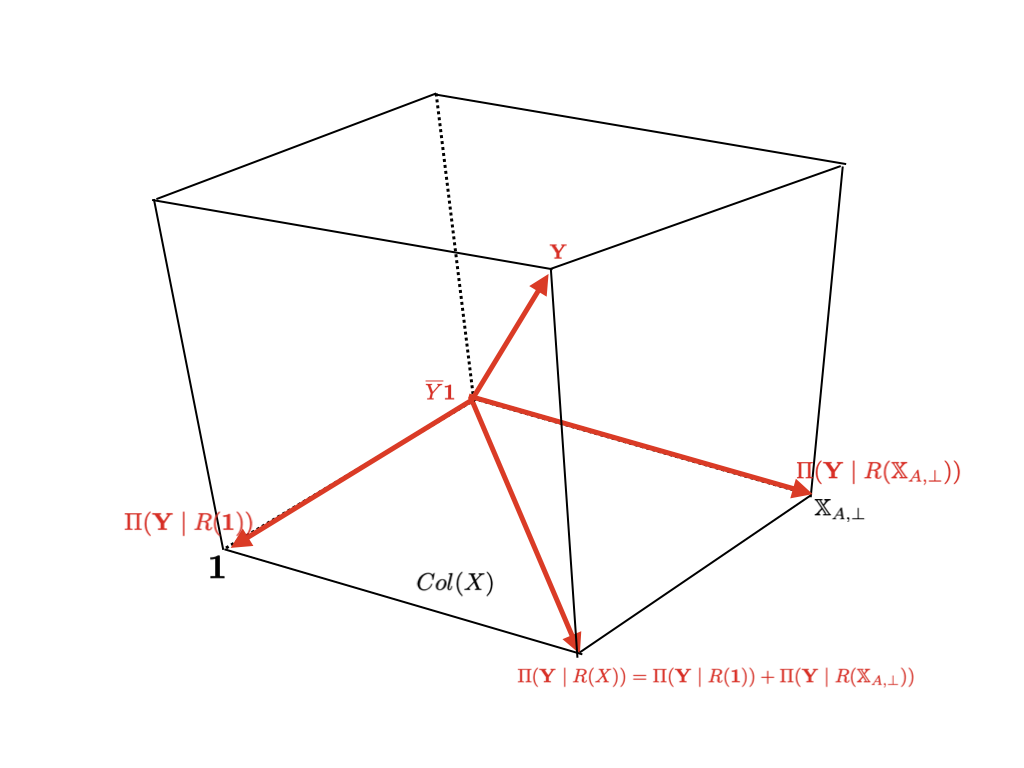
\includegraphics[width=0.7\linewidth]{images/multiple-orthogonal} 

}

\caption{Orthogonal decomposition of the column space and LSE}\label{fig:illdecomp}
\end{figure}

See Figure \ref{fig:illdecomp}. Two are orthogonal, so sum of projections onto them become LSE. In fact, \emph{each projection indicate each regression coefficient}. When we do not have orthogonal basis, however, each projection is nothing.

\begin{figure}[H]

{\centering 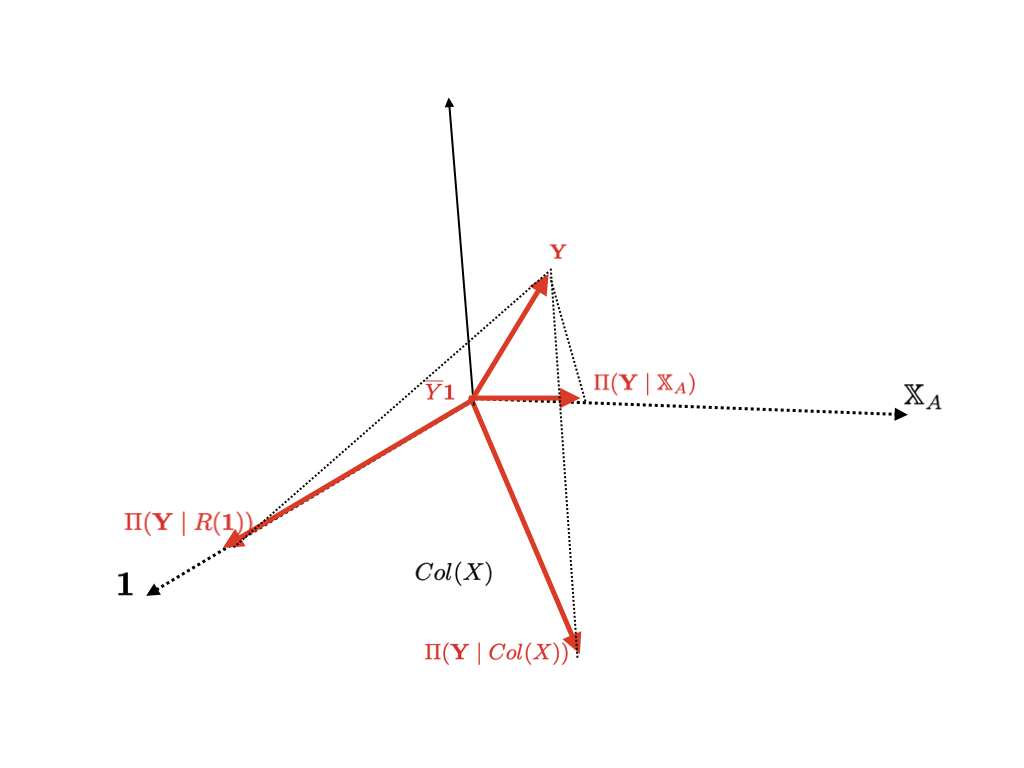
\includegraphics[width=0.7\linewidth]{images/multiple-nonorth} 

}

\caption{Non-orthongality}\label{fig:illdecomp2}
\end{figure}

So what we have done is orthogonalization.

\[\tilde{\mathbb{X}}_A = \Pi_{\mathbf{1}}\mathbb{X}_A + (\mathbb{X}_A - \Pi_{\mathbf{1}}\mathbb{X}_A)\]

\hypertarget{gram-schmidt-qr-factorization}{%
\subsection{Gram-Schmidt QR factorization}\label{gram-schmidt-qr-factorization}}

Let's briefly look at orthogonalization process. From Theorem \ref{thm:orthonormal}, we can derive following \emph{orthonormalization process}.

\BeginKnitrBlock{theorem}[Gram-Schmidt Process]
\protect\hypertarget{thm:gs}{}{\label{thm:gs} \iffalse (Gram-Schmidt Process) \fi{} }Let \(\{ \mathbf{x}_1, \ldots, \mathbf{x}_{p + 1} \}\) be a basis for the inner product space \(V\). Let

\[\mathbf{u}_1 = \bigg( \frac{1}{\lVert \mathbf{x}_1 \rVert} \bigg) \mathbf{x}_1\]

and define next \(\mathbf{u}_2, \ldots, \mathbf{u}_{p + 1}\) recursively by

\[\mathbf{u}_{k + 1} = \frac{1}{\lVert \mathbf{x}_{k + 1} - \mathbf{r}_k^{*} \rVert}(\mathbf{x}_{k + 1} - \mathbf{r}_k^{*})\]

for \(k = 1, \ldots, p\), where

\[\mathbf{r}_k^{*} = <\mathbf{x}_{k + 1}, \mathbf{u}_1> \mathbf{u}_1 + <\mathbf{x}_{k + 1}, \mathbf{u}_2 >\mathbf{u}_2 + \cdots + < \mathbf{x}_{k + 1}, \mathbf{u}_k > \mathbf{u}_k\]

is the projection of \(\mathbf{x}_{k + 1}\) onto \(sp(\{ \mathbf{u}_1, \ldots, \mathbf{u}_k \})\).

Hence, we get \(\{ \mathbf{u}_1, \ldots, \mathbf{u}_{p + 1} \}\) is an orthonormal basis for \(V\).
\EndKnitrBlock{theorem}

\begin{algorithm} \label{alg:alggs}
  \SetAlgoLined
  \SetKwInOut{Input}{input}
  \Input{basis $\{ \mathbf{x}_0, \ldots, \mathbf{x}_p \}$}
  Initialize $\mathbf{v}_0 = \mathbf{x}_0$\;
  \For{$k \leftarrow 1$ \KwTo $p$}{
    $\mathbf{u}_{k - 1} = \frac{\mathbf{v}_{k - 1}}{\lVert \mathbf{v}_{k - 1} \rVert}$\;
    $\mathbf{r}_k^{*} = <\mathbf{x}_{k + 1}, \mathbf{u}_0> \mathbf{u}_0 + <\mathbf{x}_{k + 1}, \mathbf{u}_1 >\mathbf{u}_1 + \cdots + < \mathbf{x}_{k + 1}, \mathbf{u}_k > \mathbf{u}_k$\;
    $\mathbf{v}_{k + 1} = \mathbf{x}_{k + 1} - \mathbf{r}_k^{*}$
  }
  $\mathbf{u}_p = \frac{\mathbf{v}_p}{\lVert \mathbf{v}_p \rVert}$
  \caption{Gram-schmidt process}
\end{algorithm}

Our interest is \(Col(X)\), and we can factorizae this model matrix so that it represents orthonormalization process \ref{thm:gs}.

\BeginKnitrBlock{theorem}[Gram-Schmidt QR factorization]
\protect\hypertarget{thm:gsqr}{}{\label{thm:gsqr} \iffalse (Gram-Schmidt QR factorization) \fi{} }Let \(X \in \mathbb{R}^{n \times (p + 1)}\). Then \(X\) can be factored into

\[X = QR\]

where \(Q \in \mathbb{R}^{n \times (p + 1)}\) is an orthogonal matrix, i.e.~its column vectors are orthonormal and \(R \in \mathbb{R}^{(p + 1) \times (p + 1)}\) is an upper triangular matrix whose diagonal entries are all positive.
\EndKnitrBlock{theorem}

\BeginKnitrBlock{proof}
\iffalse{} {Proof. } \fi{}Denote that this is just the representation of Gram-schmidt orthogonalization. Then it gives

\[\mathbf{u}_1 = \frac{\mathbf{x}_1}{\lVert \mathbf{x}_1 \rVert} \Rightarrow \mathbf{x}_1 = \lVert \mathbf{x}_1 \rVert \mathbf{u}_1\]

\begin{equation*}
  \begin{split}
    & \mathbf{v}_2 = \mathbf{x}_2 - <\mathbf{x}_2, \mathbf{u}_1> \mathbf{u}_1, \quad \mathbf{u}_2 = \frac{\mathbf{v}_2}{\lVert \mathbf{v}_2 \rVert} \\
    & \Rightarrow \mathbf{x}_2 = <\mathbf{x}_2, \mathbf{u}_1>\mathbf{u}_1 + \lVert \mathbf{v}_2 \rVert \mathbf{u}_2 \\
    & \Rightarrow \mathbf{x}_2 = \left[\begin{array}{c|c}
      \mathbf{u}_1 & \mathbf{u}_2
    \end{array}\right] \begin{bmatrix}
      <\mathbf{x}_2, \mathbf{u}_1> \\
      \lVert \mathbf{v}_2 \rVert
    \end{bmatrix}
  \end{split}
\end{equation*}

It procees in a simlar way to the others. Hence,

\begin{equation}
  \begin{split}
    X & = \begin{bmatrix} \mathbf{x}_1 & \cdots & \mathbf{x}_{p+1} \end{bmatrix} \\
    & = \begin{bmatrix}
      \mathbf{u}_1 & \mathbf{u}_2 & \cdots & \mathbf{u}_{p + 1}
    \end{bmatrix} \begin{bmatrix}
      \lVert \mathbf{v}_1 \rVert & < \mathbf{x}_2, \mathbf{u}_1> & < \mathbf{x}_3, \mathbf{u}_1> & \cdots & < \mathbf{x}_{p + 1}, \mathbf{u}_1> \\
      0 & \lVert \mathbf{v}_2 \rVert & < \mathbf{x}_3, \mathbf{u}_2> & \cdots & < \mathbf{x}_{p + 1}, \mathbf{u}_2> \\
      0 & 0 & \lVert \mathbf{v}_3 \rVert & \cdots & < \mathbf{x}_{p + 1}, \mathbf{u}_3> \\
      \vdots & \vdots & \vdots & \vdots & \vdots \\
      0 & 0 & 0 & 0 & \lVert \mathbf{v}_{p + 1} \rVert
    \end{bmatrix} \\
    & \equiv QR
  \end{split}
  \label{eq:qrrep}
\end{equation}
\EndKnitrBlock{proof}

Look again the equation in Theorem \ref{thm:gs}. In each process \(k\), the projection is done to the \((k - 1)\)-dimensional space. In other words, as process goes through, dimension increases. So we try to project each vector only in 1-dimension each step.

\BeginKnitrBlock{theorem}[Modified Gram-Schmidt Process]
\protect\hypertarget{thm:modgs}{}{\label{thm:modgs} \iffalse (Modified Gram-Schmidt Process) \fi{} }Let \(\{ \mathbf{x}_1, \ldots, \mathbf{x}_{p + 1} \}\) be a basis for the inner product space \(V\) and let \(\{ \mathbf{q}_1, \ldots, \mathbf{q}_{p + 1} \}\) be an orthonormal basis.

Set \(\mathbf{q}_1 = \frac{\mathbf{x}_1}{\lVert \mathbf{x}_1 \rVert}\). Then consider \(sp(\{ \mathbf{q}_1 \})\).

In the first step, make every \(\{ \mathbf{x}_2, \ldots, \mathbf{x}_{p + 1} \}\) orthogonal to \(\mathbf{q}_1\).

\[\mathbf{x}_k^{(1)} = \mathbf{x}_k - (\mathbf{q}_1^T \mathbf{x}_k)\mathbf{q}_1, \quad k = 2, \ldots, p + 1\]

So we get orthogonal set \(\{ \mathbf{q}_1, \mathbf{x}_2^{(1)}, \ldots, \mathbf{x}_{p + 1}^{(1)} \}\). Next, set \(\mathbf{q}_2 = \frac{\mathbf{x}^{(1)}}{\lVert \mathbf{x}_2^{(2)} \rVert}\). Consider \(sp(\{ \mathbf{q}_2 \})\). Since we have \(\mathbf{q}_1 \perp \mathbf{q}_2\),

\[\mathbf{x}_k^{(2)} = \mathbf{x}_k^{(1)} - (\mathbf{q}_2^T \mathbf{x}_k^{(1)})\mathbf{q}_2 \perp \mathbf{q}_2 , \quad k = 3, \ldots, p + 1\]

Thus, get \(\{ \mathbf{q}_1, \mathbf{q}_2, \mathbf{x}_3^{(2)}, \ldots, \mathbf{x}_{p + 1}^{(2)} \}\). \(\mathbf{q}_3, \ldots, \mathbf{q}_{p + 1}\) are successively determined in a similary way.

At the last step, set

\[\mathbf{q}_{p + 1} = \frac{\mathbf{x}_{p + 1}^{(p)}}{\lVert \mathbf{x}_{p + 1}^{(p)} \rVert}\]
\EndKnitrBlock{theorem}

Since each projection is done in 1-dimension, the algorithm becomes more understandable. Consider

\[
Q = \begin{bmatrix}
  \mathbf{q}_1 & \mathbf{q}_2 & \cdots \mathbf{q}_{p + 1}
\end{bmatrix} \in \mathbb{R}^{n \times (p + 1)} \quad \text{orthogonal}
\]

and

\[
R = [r_{kj}] = \begin{bmatrix}
  r_{11} & r_{12} & \cdots & r_{1,p+1} \\
  0 & r_{22} & \cdots & r_{2, p+1} \\
  0 & 0 & \cdots & r_{3,p+1} \\
  \vdots & \vdots & \vdots & \vdots \\
  0 & 0 & 0 & r_{p+1, p+1}
\end{bmatrix} \in \mathbb{R}^{(p+1) \times (p + 1)}
\]

We can perform \(QR\) factorization by following step.

\begin{algorithm} \label{alg:algqr}
  \SetAlgoLined
  \For{$k \leftarrow 1$ \KwTo $(p + 1)$}{
    $r_{kk} = \lVert \mathbf{x}_{k} \rVert$\;
    $\mathbf{q}_k = \frac{\mathbf{x}_k}{r_{kk}}$\;
    \For{$j \leftarrow 1$ \KwTo $(p + 1)$}{
      $r_{kj} = \mathbf{q}_k^T\mathbf{x}_j$\;
      $\mathbf{x}_j = \mathbf{x}_j - r_{kj}\mathbf{q}_k$\;
    }
  }
  \caption{QR decomposition for modified G-S process}
\end{algorithm}

This \emph{orthonormal basis} gives some useful facts with least squares problem \citep{Leon:2014aa}.

\hypertarget{successive-orthogonalization}{%
\subsection{Successive orthogonalization}\label{successive-orthogonalization}}

In fact, G-S process \(\ref{alg:alggs}\) is equivalent to succesive orthogonalization, i.e.~regress(project) \(\mathbf{x}_j\) onto the others \citep{Hastie:2013aa}.

\begin{algorithm} \label{alg:algorth}
  \SetAlgoLined
  Initialize $\mathbf{v}_0 = \mathbf{1}$\;
  \For{$k \leftarrow 1$ \KwTo $p$}{
    Regress $\mathbf{x}_k$ on $\mathbf{q}_0, \ldots, \mathbf{q}_{k - 1}$\;
    $\hat\beta_{lk} = \frac{<\mathbf{v}_l, \mathbf{x}_k>}{< \mathbf{v}_l, \mathbf{v}_l>}, l = 0, \ldots, k - 1$\;
    Residual $\mathbf{v}_k = \mathbf{x}_k - \sum\limits_{l = 0}^{k - 1}\hat\beta_{lk}\mathbf{v}_k$\;
  }
  Regress $\mathbf{Y}$ on $\mathbf{v}_p$
  \caption{Successive orthogonalization}
\end{algorithm}

Now we can solve least squares problem using QR decomposition. Recall that

\[X = QR\]

as specified in Theorem \ref{thm:gsqr}. Then normal equation implies that

\begin{equation}
  \begin{split}
    & (X^TX)\boldsymbol{\hat\beta} = X^T\mathbf{Y} \\
    & \Leftrightarrow R^TQ^TQR \boldsymbol{\hat\beta} = R^TQ^T \mathbf{Y} \\
    & \Leftrightarrow R^TR \boldsymbol{\hat\beta} = R^TQ^T \mathbf{Y} \qquad \because Q^TQ = I \\
    & \Leftrightarrow R \boldsymbol{\hat\beta} = Q^T \mathbf{Y} \qquad \text{if}\: R \:\text{is invertible}
  \end{split}
  \label{eq:qrbeta}
\end{equation}

Hence,

\begin{equation}
  \boldsymbol{\hat\beta} = R^{-1}Q^T\mathbf{Y}
  \label{eq:qrhat}
\end{equation}

It follows that

\begin{equation}
  \mathbf{\hat{Y}} = (QR)\boldsymbol{\hat\beta} = QQ^T\mathbf{Y}
  \label{eq:qrfit}
\end{equation}

Let's compare the result. Base function \texttt{qr()} give the QR factorization. Given this object, we can get each \(Q\) and \(R\) by \texttt{qr.Q()} and \texttt{qr.R()}.

\begin{Shaded}
\begin{Highlighting}[]
\NormalTok{cem_qr <-}
\StringTok{  }\NormalTok{cem }\OperatorTok\StringTok{ }
\StringTok{  }\KeywordTok{model.matrix}\NormalTok{(y }\OperatorTok{~}\StringTok{ }\NormalTok{., }\DataTypeTok{data =}\NormalTok{ .) }\OperatorTok\StringTok{ }
\StringTok{  }\KeywordTok{qr}\NormalTok{()}
\NormalTok{cem_q <-}\StringTok{ }\KeywordTok{qr.Q}\NormalTok{(cem_qr)}
\NormalTok{cem_r <-}\StringTok{ }\KeywordTok{qr.R}\NormalTok{(cem_qr)}
\end{Highlighting}
\end{Shaded}

Using Equation \eqref{eq:qrhat}, we get each coefficient as follow.

\begin{Shaded}
\begin{Highlighting}[]
\KeywordTok{solve}\NormalTok{(cem_r) }\OperatorTok\StringTok{ }\KeywordTok{t}\NormalTok{(cem_q) }\OperatorTok\StringTok{ }\NormalTok{cem}\OperatorTok{$}\NormalTok{y}
\CommentTok{#>               [,1]}
\CommentTok{#> (Intercept) 62.405}
\CommentTok{#> x1           1.551}
\CommentTok{#> x2           0.510}
\CommentTok{#> x3           0.102}
\CommentTok{#> x4          -0.144}
\end{Highlighting}
\end{Shaded}

On the other hand, \texttt{lm()} gives the following result.

\begin{Shaded}
\begin{Highlighting}[]
\KeywordTok{lm}\NormalTok{(y }\OperatorTok{~}\StringTok{ }\NormalTok{., }\DataTypeTok{data =}\NormalTok{ cem)}
\CommentTok{#> }
\CommentTok{#> Call:}
\CommentTok{#> lm(formula = y ~ ., data = cem)}
\CommentTok{#> }
\CommentTok{#> Coefficients:}
\CommentTok{#> (Intercept)           x1           x2           x3           x4  }
\CommentTok{#>      62.405        1.551        0.510        0.102       -0.144}
\end{Highlighting}
\end{Shaded}

We can check the result is same. In fact, \texttt{lm()} fits the model by default \texttt{method\ =\ "qr"}.

\begin{quote}
the method to be used; for fitting, currently only method = ``qr'' is supported; method = ``model.frame'' returns the model frame (the same as with model = TRUE, see below).
\end{quote}

By default and only way, \texttt{lm()} fits the model using \(QR\) factorization. What does this orthogonal basis mean? For simplicity, consider simple linear regression problem.

\begin{figure}[H]

{\centering 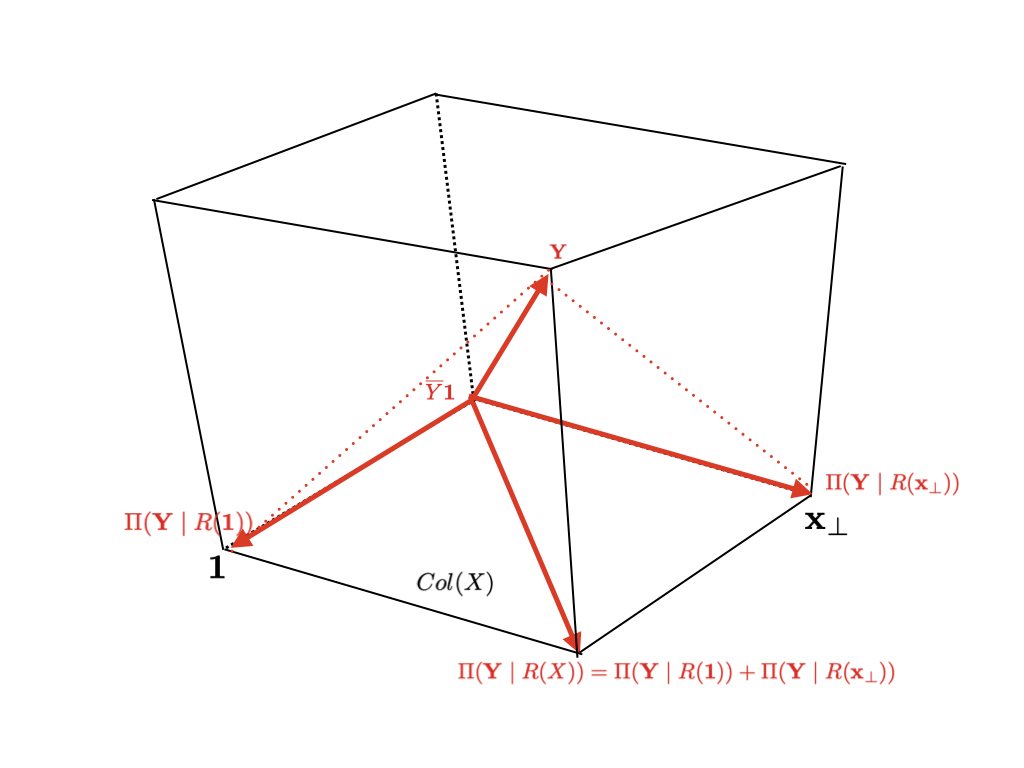
\includegraphics[width=0.7\linewidth]{images/multiple-qr1} 

}

\caption{Orthogonalized basis}\label{fig:qrpng}
\end{figure}

\begin{figure}[H]

{\centering 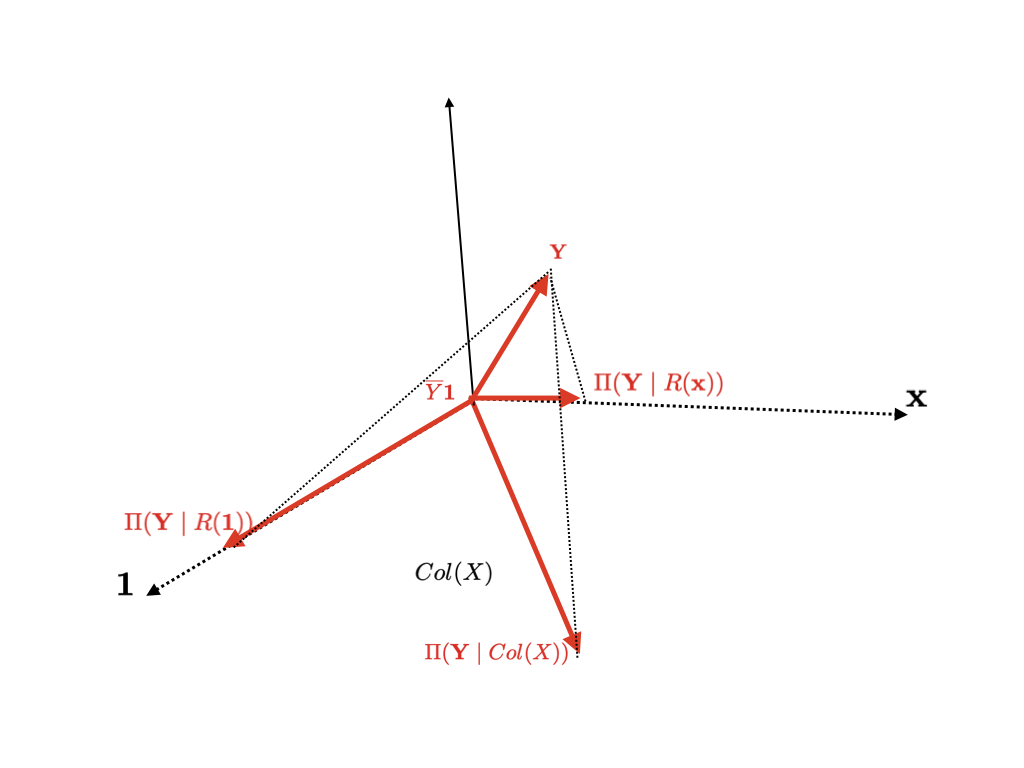
\includegraphics[width=0.7\linewidth]{images/multiple-qr2} 

}

\caption{Non-orthogonal basis}\label{fig:qrpng2}
\end{figure}

See Figure \ref{fig:qrpng}. By construction, projection onto each basis is same as \(\hat\beta_0\) and \(\hat\beta_1\). In Figure \ref{fig:qrpng2}, however, each projection is not regression coefficient.

\begin{figure}[H]

{\centering 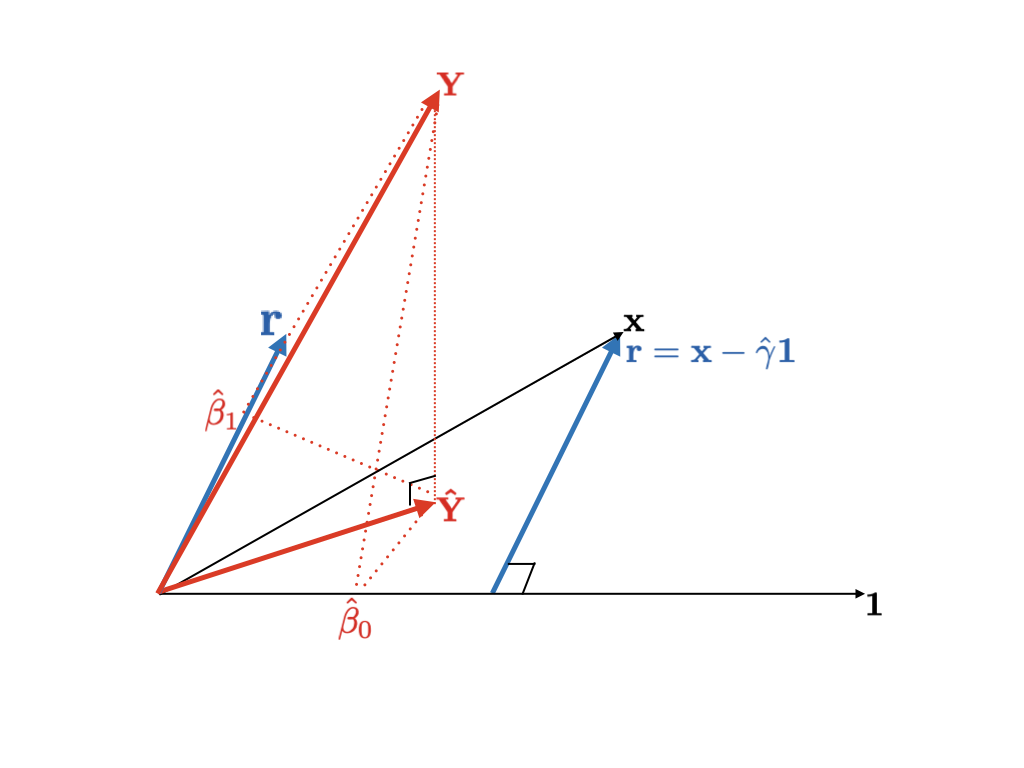
\includegraphics[width=0.7\linewidth]{images/multiple-qr3} 

}

\caption{QR decomposition for model matrix}\label{fig:simpledraw3}
\end{figure}

Regress \(\mathbf{x}\) onto \(\mathbf{1}\). Its residual can be a new orthogonalized predictor.

\hypertarget{properties-of-lse}{%
\subsection{Properties of LSE}\label{properties-of-lse}}

We have seen how we extend point estimator \(\boldsymbol{\hat\beta}\). In turn, we can check this is unbiased, and BLUE.

\BeginKnitrBlock{proposition}[Expectation and Variance]
\protect\hypertarget{prp:multbmoment}{}{\label{prp:multbmoment} \iffalse (Expectation and Variance) \fi{} }\(\boldsymbol{\hat\beta}\) is unbiased.

\begin{enumerate}
  \item $E\boldsymbol{\hat\beta} = \boldsymbol\beta$
  \item $Var\boldsymbol{\hat\beta} = \sigma^2(X^TX)^{-1}$
\end{enumerate}
\EndKnitrBlock{proposition}

\BeginKnitrBlock{proof}
\iffalse{} {Proof. } \fi{}\begin{equation*}
  \begin{split}
    E\boldsymbol{\hat\beta} & = E\bigg( (X^TX)^{-1}X^T\mathbf{Y} \bigg) \\
    & = (X^TX)^{-1}X^T E\mathbf{Y} \\
    & = (X^TX)^{-1}X^T X\boldsymbol\beta \\
    & = \boldsymbol\beta
  \end{split}
\end{equation*}

Hence, \(\boldsymbol{\hat\beta}\) is unbiased.

\begin{equation*}
  \begin{split}
    Var\boldsymbol{\hat\beta} & = Var\bigg( (X^TX)^{-1}X^T\mathbf{Y} \bigg) \\
    & = (X^TX)^{-1}X^T Var(\mathbf{Y}) X(X^TX)^{-1} \\
    & = (X^TX)^{-1}X^T(\sigma^2 I)X(X^TX)^{-1} \\
    & = \sigma^2 (X^TX)^{-1}
  \end{split}
\end{equation*}
\EndKnitrBlock{proof}

Since the variance of LSE have been revealed, now we want to know if this is the lowest one among estimators. Gauss-Markov theorem states that LSE has the lowest variance among linear unbiased estimators for \(\boldsymbol\beta\), so called the \textbf{best linear unbiased estimator (BLUE)}.

\BeginKnitrBlock{theorem}[Gauss-Markov Theorem]
\protect\hypertarget{thm:multgm}{}{\label{thm:multgm} \iffalse (Gauss-Markov Theorem) \fi{} }\(\boldsymbol{\hat\beta} = (X^TX)^{-1}X^T\mathbf{Y}\) is BLUE, i.e.

For any \(\tilde{\boldsymbol\beta} \in \Omega \equiv \{ \tilde{\boldsymbol\beta} : \tilde{\boldsymbol\beta} = C\mathbf{Y} , E\tilde{\boldsymbol\beta} = \boldsymbol\beta \}\),

\[Var(\boldsymbol{\hat\beta}) \le Var(\tilde{\boldsymbol\beta})\]
\EndKnitrBlock{theorem}

\BeginKnitrBlock{proof}
\iffalse{} {Proof. } \fi{}Let \(\tilde{\boldsymbol\beta} \in \Omega \equiv \{ \tilde{\boldsymbol\beta} : \tilde{\boldsymbol\beta} = C\mathbf{Y} , E\tilde{\boldsymbol\beta} = \boldsymbol\beta \}\)

Claim: \(Var(\tilde{\boldsymbol\beta}) - Var(\boldsymbol{\hat\beta})\) is non-negative definite.

Note that \(\boldsymbol{\hat\beta}\) is the one with \(C = (X^TX)^{-1}X^T\).

Set \(D := C - (X^TX)^{-1}X^T\). From unbiasedness,

\begin{equation*}
  \begin{split}
    E\tilde{\boldsymbol\beta} & = CE\mathbf{Y} \\
    & = CX\boldsymbol\beta \\
    & = \Big( (X^TX)^{-1}X^T + D \Big)X\boldsymbol\beta \\
    & = \boldsymbol\beta + DX\boldsymbol\beta \\
    & = \boldsymbol\beta
  \end{split}
\end{equation*}

Since \(\forall \boldsymbol\beta \in \mathbb{R}^{p + 1} : DX \boldsymbol\beta = \mathbf{0}\),

\begin{equation} \label{eq:prgm}
  DX = 0
\end{equation}

\begin{equation*}
  \begin{split}
    Var\tilde{\boldsymbol\beta} & = Var(C\mathbf{Y}) \\
    & = \sigma^2CC^T \\
    & = \sigma^2\Big( (X^TX)^{-1}X^T + D \Big) \Big( (X^TX)^{-1}X^T + D \Big)^T \\
    & = \sigma^2\Big( (X^TX)^{-1} + DX(X^TX)^{-1} + (X^TX)^{-1}X^TD^T + DD^T \Big) \\
    & = \sigma^2\Big( (X^TX)^{-1} + DD^T \Big) \qquad \because \eqref{eq:prgm} \\
    & = Var\boldsymbol{\hat\beta} + \sigma^2DD^T
  \end{split}
\end{equation*}

Note that \(DD^T\) is non-negative definite. Hence,

\[Var\tilde{\boldsymbol\beta} - Var\boldsymbol{\hat\beta} = \sigma^2DD^T\]

is non-negative definite. This completes the proof.
\EndKnitrBlock{proof}

As in simple linear regression setting, we define \emph{residuals} and explain \(\sigma^2\).

\BeginKnitrBlock{definition}[Residuals]
\protect\hypertarget{def:multres}{}{\label{def:multres} \iffalse (Residuals) \fi{} }Let \(\hat{\mathbf{Y}} = (\hat{Y_1}, \ldots, \hat{Y_n})^T\) with \(\hat{Y_i} = \hat\beta_0 + \hat\beta_1 x_{i1} + \cdots + \hat\beta_px_{ip}\). Then the residual is defined by

\[\mathbf{e} := (\ldots,Y_i - \hat\beta_0 - \hat\beta_1 x_{i1} - \cdots - \hat\beta_px_{ip}, \ldots)^T = \mathbf{Y} - \hat{\mathbf{Y}} \in \mathbb{R}^n\]
\EndKnitrBlock{definition}

Extending the simple setting, we estimate \(\sigma^2\) with inner product of residuals divided by its degrees of freedom, i.e.~\emph{MSE}. The degrees of freedom becomes \(n - \text{the number of coefficients}\). Thus, \(n - (p + 1) = n - p - 1\).

\BeginKnitrBlock{proposition}[Estimation of $\sigma^2$]
\protect\hypertarget{prp:multsigma}{}{\label{prp:multsigma} \iffalse (Estimation of \(\sigma^2\)) \fi{} }Let \(\mathbf{e} = \mathbf{Y} - \hat{\mathbf{Y}}\) be residuals as in Definition \ref{def:multres}. Then

\[\hat\sigma^2 = \frac{\lVert \mathbf{e} \rVert}{n - p - 1}\]
\EndKnitrBlock{proposition}

The reason we divide with degrees of freedom is to make \(\hat\sigma^2\) unbiased.

\BeginKnitrBlock{proposition}[Mean of $\hat\sigma^2$]
\protect\hypertarget{prp:multsigmean}{}{\label{prp:multsigmean} \iffalse (Mean of \(\hat\sigma^2\)) \fi{} }\(\hat\sigma^2\) is unbiased, i.e.

\[E\bigg( \lVert \mathbf{Y} - \hat{\mathbf{Y}} \rVert^2 \bigg) = (n - p - 1)\sigma^2\]
\EndKnitrBlock{proposition}

\BeginKnitrBlock{proof}
\iffalse{} {Proof. } \fi{}Since \(\mathbf{Y} = \Pi_X\mathbf{Y}\),

\begin{equation*}
  \begin{split}
    \lVert \mathbf{Y} - \hat{\mathbf{Y}} \rVert^2 & = \lVert (I - \Pi_X)\mathbf{Y} \rVert^2 \\
    & = \mathbf{Y}^T(I - \Pi_X)^T(I - \Pi_X)\mathbf{Y} \\
    & = \mathbf{Y}^T (I - \Pi_X)\mathbf{Y} \qquad \because (I - \Pi_X): \text{symmetric idempotent}
  \end{split}
\end{equation*}

Since \(\mathbf{Y}^T (I - \Pi_X)\mathbf{Y} \in \mathbb{R}\),

\begin{equation*}
  \begin{split}
    \mathbf{Y}^T (I - \Pi_X)\mathbf{Y} & = tr\bigg( \mathbf{Y}^T (I - \Pi_X)\mathbf{Y} \bigg) \\
    & = tr\bigg( (I - \Pi_X)\mathbf{Y} \mathbf{Y}^T \bigg)
  \end{split}
\end{equation*}

Then

\begin{equation*}
  \begin{split}
    E\lVert \mathbf{Y} - \hat{\mathbf{Y}} \rVert^2 & = E\Big[ \mathbf{Y}^T (I - \Pi_X)\mathbf{Y} \Big] \\
    & = E\bigg[ tr\Big( (I - \Pi_X)\mathbf{Y} \mathbf{Y}^T \Big) \bigg] \\
    & = tr\bigg( (I - \Pi_X) \underset{(\ast)}{\underline{E\Big[ \mathbf{Y} \mathbf{Y}^T \Big]}} \bigg)
  \end{split}
\end{equation*}

Consider \((\ast)\).

\begin{equation*}
  \begin{split}
    E(\mathbf{Y}\mathbf{Y}^T) & = Var\mathbf{Y} + (E\mathbf{Y})(E\mathbf{Y})^T \\
    & = \sigma^2 I + X\boldsymbol\beta\boldsymbol\beta^T X^T
  \end{split}
\end{equation*}

Hence,

\begin{equation*}
  \begin{split}
    E\lVert \mathbf{Y} - \hat{\mathbf{Y}} \rVert^2 & = tr\bigg( (I - \Pi_X) E\Big[ \mathbf{Y} \mathbf{Y}^T \Big] \bigg) \\
    & = tr\bigg((I - \Pi_X)\sigma^2 + (I - \Pi_X)X\boldsymbol\beta\boldsymbol\beta^T X^T \bigg) \\
    & = tr\bigg( (I - \Pi_X)\sigma^2 \bigg) + tr\bigg( \boldsymbol\beta^T X^T(I - \Pi_X)X\boldsymbol\beta \bigg) \qquad \because (I - \Pi_X)X\boldsymbol\beta = X\boldsymbol\beta - X\boldsymbol\beta = 0 \\
    & = tr\bigg( (I - \Pi_X)\sigma^2 \bigg) \\
    & = (n - p - 1)\sigma^2 \qquad \because \begin{cases} tr(I) = n \\ tr(\Pi_X) = p + 1 \end{cases}
  \end{split}
\end{equation*}
\EndKnitrBlock{proof}

In this proposition, we have used model matrix directly. Instead, we can use Equation \eqref{eq:qrhat} for simplicity.

\BeginKnitrBlock{proposition}[Variance using QR decomposition]
\protect\hypertarget{prp:qrmoment}{}{\label{prp:qrmoment} \iffalse (Variance using QR decomposition) \fi{} }Let \(X = QR\). Then \(\boldsymbol{\hat\beta} = R^{-1}Q^T\mathbf{Y}\). It follows that

\[Var\boldsymbol{\hat\beta} = \sigma^2(R^TR)^{-1}\]
\EndKnitrBlock{proposition}

\BeginKnitrBlock{proof}
\iffalse{} {Proof. } \fi{}It proceeds in a similar way for \(\boldsymbol{\hat\beta} = R^{-1}Q^T\mathbf{Y}\).

\begin{equation*}
  \begin{split}
    Var\boldsymbol{\hat\beta} & = Var\bigg( R^{-1}Q^T\mathbf{Y} \bigg) \\
    & = R^{-1}Q^T Var(\mathbf{Y}) Q(R^T)^{-1} \\
    & = R^{-1}Q^T (\sigma^2 I) Q(R^T)^{-1} \\
    & = \sigma^2 (R^TR)^{-1} \qquad \because Q^TQ = I \\
  \end{split}
\end{equation*}
\EndKnitrBlock{proof}

\BeginKnitrBlock{proposition}[QR representation for residual]
\protect\hypertarget{prp:qrres}{}{\label{prp:qrres} \iffalse (QR representation for residual) \fi{} }Let \(X = QR\). Then

\[\mathbf{e} = (I - QQ^T)\mathbf{Y}\]
\EndKnitrBlock{proposition}

\BeginKnitrBlock{proof}
\iffalse{} {Proof. } \fi{}From Equation \eqref{eq:qrfit},

\[\Pi_X = QQ^T\]

Hence,

\[\mathbf{e} = (I - \Pi_X)\mathbf{Y} = (I - QQ^T)\mathbf{Y}\]
\EndKnitrBlock{proof}

On Figure \ref{fig:simpledraw3}, we can see these relations. Operation \(Q^T\mathbf{Y}\) is just projection to each orthogonal basis. \(Q\) sums these projection so that we get \(\mathbf{\hat{Y}}\) which projection of \(\mathbf{Y}\) onto the column space of model matrix.

\begin{figure}[H]

{\centering 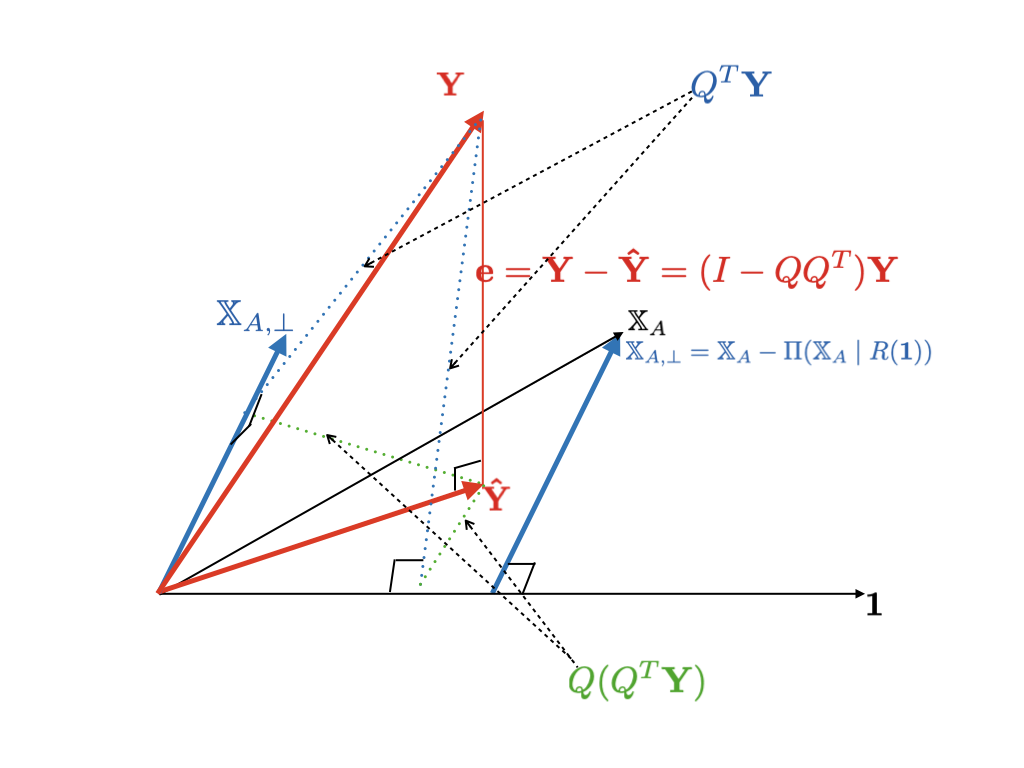
\includegraphics[width=0.7\linewidth]{images/multiple-residual} 

}

\caption{Residual vector}\label{fig:multresfig}
\end{figure}

\hypertarget{mean-response-and-response-1}{%
\subsection{Mean response and response}\label{mean-response-and-response-1}}

Let \(\mathbf{z} = (z_1, \ldots, z_p)^T\).

\BeginKnitrBlock{theorem}[Estimation of the mean response]
\protect\hypertarget{thm:multmeanres}{}{\label{thm:multmeanres} \iffalse (Estimation of the mean response) \fi{} }\[\hat\mu_z = \hat\beta_0 + \mathbf{z}^T\boldsymbol{\hat\beta}_A\]
\EndKnitrBlock{theorem}

\BeginKnitrBlock{theorem}[(out of sample) Prediction of a response]
\protect\hypertarget{thm:multpred}{}{\label{thm:multpred} \iffalse ((out of sample) Prediction of a response) \fi{} }\[\hat{Y}_z = \hat\beta_0 + \mathbf{z}^T \boldsymbol{\hat\beta}_Z\]
\EndKnitrBlock{theorem}

\BeginKnitrBlock{proposition}[Residual vector]
\protect\hypertarget{prp:multresprop}{}{\label{prp:multresprop} \iffalse (Residual vector) \fi{} }Let \(\mathbf{e} = (I - \Pi_X)\mathbf{Y}\). Then

\begin{enumerate}
  \item $Var(\mathbf{e}) = \sigma^2(I - \Pi_X)$
  \item $\mathbf{e} \perp \mathbf{\hat{Y}}$
\end{enumerate}
\EndKnitrBlock{proposition}

\BeginKnitrBlock{proof}[$Var(\mathbf{e})$]
\iffalse{} {Proof (\(Var(\mathbf{e})\)). } \fi{}\begin{equation*}
  \begin{split}
    Var(\mathbf{e}) & = Var\Big( (I - \Pi_X)\mathbf{Y} \Big) \\
    & = (I - \Pi_X) Var(\mathbf{Y}) (I - \Pi_X)^T \\
    & = \sigma^2 (I - \Pi_X) \qquad \because (I - \Pi_X) \:\text{symmetric itempotent}
  \end{split}
\end{equation*}
\EndKnitrBlock{proof}

\BeginKnitrBlock{proof}[$\mathbf{e} \perp \mathbf{\hat{Y}}$]
\iffalse{} {Proof (\(\mathbf{e} \perp \mathbf{\hat{Y}}\)). } \fi{}Note that

\[\mathbf{e} \in Col(X)^{\perp}\]

From the properties of projection, we have

\begin{equation}
  \begin{cases}
    \mathbf{e} \perp \mathbf{1} \\
    \mathbf{e} \perp \mathbf{x}_j & \forall j = 1, 2, \ldots, p
  \end{cases}
  \label{eq:multnormaleq}
\end{equation}

Since \(\hat{Y_i} = \hat\beta_0 + \hat\beta_1 x_{i1} + \cdots + \hat\beta_p x_{ip}\),

\[\mathbf{e} \perp \mathbf{\hat{Y}}\]
\EndKnitrBlock{proof}

Equation \eqref{eq:multnormaleq} is another form of the \emph{normal equation}.

\BeginKnitrBlock{remark}
\iffalse{} {Remark. } \fi{}The least squares regression line \(\{ (\mathbf{z}, y) : y = \hat\beta_0 + \mathbf{z}^T\hat\beta_A \}\) always passes through

\[\bigg( \frac{1}{n} \mathbb{X}_A^T \mathbf{1}, \overline{Y} \bigg)\]

In simple linear regression setting,

\[(\overline{x}, \overline{Y})\]
\EndKnitrBlock{remark}

\BeginKnitrBlock{proof}
\iffalse{} {Proof. } \fi{}First consider \(p = 1\). Normal equation gives directly that

\[\hat\beta_0 = \overline{Y} - \hat\beta_1 \overline{x}\]

Thus,

\[\overline{Y} = \hat\beta_0 + \hat\beta_1 \overline{x}\]

We now give more general proof, i.e.~for \(p \ge 1\).

Claim: \(\overline{Y} = \hat\beta_0 + \bigg(\frac{1}{n} \mathbb{X}_A^T \mathbf{1} \bigg)^T \boldsymbol{\hat\beta}_A\)

From Equation \eqref{eq:orthbeta},

\[\hat\beta_0 = \overline{Y} - \frac{1}{n}\mathbf{1}^T\mathbb{X}_A\boldsymbol{\hat\beta}_A\]

It follows that

\[\overline{Y} = \hat\beta_0 + \frac{1}{n}\mathbf{1}^T\mathbb{X}_A\boldsymbol{\hat\beta}_A\]

This completes the proof.
\EndKnitrBlock{proof}

\hypertarget{analysis-of-variance-1}{%
\section{Analysis of Variance}\label{analysis-of-variance-1}}

\hypertarget{decomposition-of-sst}{%
\subsection{Decomposition of SST}\label{decomposition-of-sst}}

We have

\begin{itemize}
\tightlist
\item
  \(SST = \lVert \mathbf{Y} - \overline{Y}\mathbf{1} \rVert^2 = \mathbf{Y}^T(I - \Pi_{\mathbf{1}})\mathbf{Y}\)
\item
  \(SSR = \lVert \mathbf{\hat{Y}} - \overline{Y}\mathbf{1} \rVert^2 = \mathbf{Y}^T(\Pi_X - \Pi_{\mathbf{1}})\mathbf{Y}\)
\item
  \(SSE = \lVert \mathbf{Y} - \mathbf{\hat{Y}} \rVert^2 = \mathbf{Y}^T(I - \Pi_X)\mathbf{Y}\)
\end{itemize}

\begin{figure}[H]

{\centering 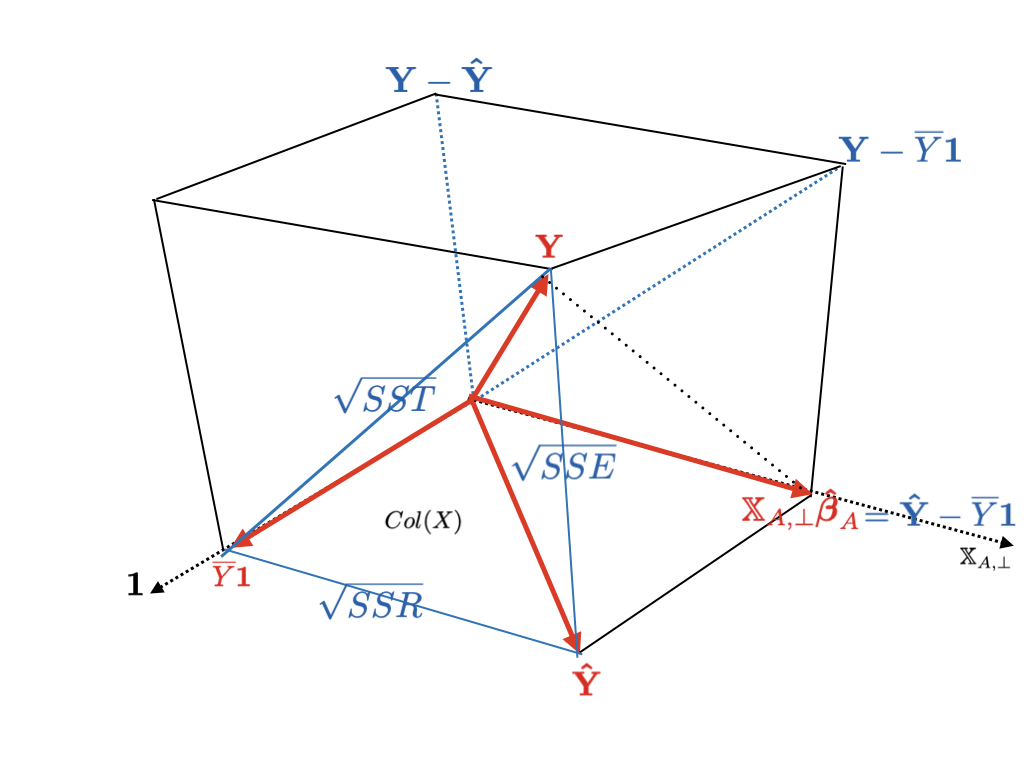
\includegraphics[width=0.7\linewidth]{images/multiple-anova} 

}

\caption{Decomposition of SST}\label{fig:mdecomp}
\end{figure}

In Figure \ref{fig:mdecomp}, Pythagorean law gives

\[SST = SSR + SSE\]

\BeginKnitrBlock{lemma}
\protect\hypertarget{lem:unnamed-chunk-71}{}{\label{lem:unnamed-chunk-71} }Let \(X = [\mathbf{1} \mid \mathbb{X}_A]\) and let \(\mathbb{X}_{A, \perp} = \mathbb{X}_A - \Pi_{\mathbf{1}}\mathbb{X}_A\). Then

\[\mathbf{\hat{Y}} - \overline{Y}\mathbf{1} = \mathbb{X}_{A, \perp}\boldsymbol{\hat\beta}_A\]
\EndKnitrBlock{lemma}

\BeginKnitrBlock{proof}
\iffalse{} {Proof. } \fi{}Note that \(\mathbf{1} \perp \mathbb{X}_{A, \perp}\).

Recall that

\[\Pi(\mathbf{Y} \mid R(\mathbf{1})) = \mathbf{1}(\mathbf{1}^T\mathbf{1})^{-1}\mathbf{1}^T\mathbf{Y} = \overline{Y}\mathbf{1}\]

From Theorem \ref{thm:orthdecomp},

\begin{equation*}
  \begin{split}
    \mathbf{\hat{Y}} & = \Pi(\mathbf{Y} \mid R(\mathbf{1})) + \Pi(\mathbf{Y} \mid R(\mathbb{X}_{A,\perp})) \\
    & = \overline{Y}\mathbf{1} + \mathbb{X}_{A,\perp}\boldsymbol{\hat\beta}_A
  \end{split}
\end{equation*}

Hence,

\[\mathbf{\hat{Y}} - \overline{Y}\mathbf{1} = \mathbb{X}_{A,\perp}\boldsymbol{\hat\beta}_A\]
\EndKnitrBlock{proof}

\hypertarget{distributions}{%
\subsection{Distributions}\label{distributions}}

\BeginKnitrBlock{proposition}[Distribution of SS]
\protect\hypertarget{prp:ssdist}{}{\label{prp:ssdist} \iffalse (Distribution of SS) \fi{} }Extending for \(p > 1\), we can get each result.

\begin{enumerate}
  \item $\frac{SSE}{\sigma^2} \sim \chi^2(n - p - 1)$
  \item $\frac{SSR}{\sigma^2} \sim \chi^2(p, \delta), \quad \delta = \frac{\boldsymbol\beta^TX^T(\Pi_X - \Pi_{\mathbf{1}})X\boldsymbol\beta}{\sigma^2}$
  \item $SSR \perp\!\!\!\perp SSE$
  \item $SSE \perp\!\!\!\perp\boldsymbol{\hat\beta}$
  \item $\frac{SST}{\sigma^2} \sim \chi^2(n - 1, \delta), \quad \delta = \frac{\boldsymbol\beta^TX^T(I - \Pi_{\mathbf{1}})X\boldsymbol\beta}{\sigma^2}$
\end{enumerate}
\EndKnitrBlock{proposition}

\BeginKnitrBlock{proof}[Distribution of SSE]
\iffalse{} {Proof (Distribution of SSE). } \fi{}Note that

\[SSE = \mathbf{Y}^T(I - \Pi_X)\mathbf{Y}\]

From Theorem \ref{thm:quaddist},

\[K = rank(I - \Pi_X) = tr(I - \Pi_X) = n - rank(\Pi_X) = n - p - 1\]

\(\delta\) proof is exactly same as Proposition \ref{prp:ssedist}.

\begin{equation*}
  \begin{split}
    \delta & = \bigg(\frac{X\boldsymbol\beta}{\sigma}\bigg)^T (I - \Pi_X) \bigg(\frac{X\boldsymbol\beta}{\sigma}\bigg) \\
    & = \frac{\boldsymbol\beta^TX^TX\boldsymbol\beta}{\sigma^2} - \frac{(\boldsymbol\beta^TX^T)X(X^TX)^{-1}X^T(X\boldsymbol\beta)}{\sigma^2} \\
    & = \frac{\boldsymbol\beta^TX^TX\boldsymbol\beta}{\sigma^2} - \frac{\boldsymbol\beta^TX^TX\boldsymbol\beta}{\sigma^2} \\
    & = 0
  \end{split}
\end{equation*}

Hence, \(\delta = 0\).
\EndKnitrBlock{proof}

\BeginKnitrBlock{proof}[Distribution of SSR]
\iffalse{} {Proof (Distribution of SSR). } \fi{}Note that

\[SSR = \mathbf{Y}^T(\Pi_X - \Pi_{\mathbf{1}})\mathbf{Y}\]

From Theorem \ref{thm:quaddist},

\[K = rank(\Pi_X - \Pi_{\mathbf{1}}) = tr(\Pi_X) - tr(\Pi_{\mathbf{1}}) = rank(\Pi_X) - rank(\Pi_{\mathbf{1}}) = p + 1 - 1 = p\]

\(\delta\) proof is exactly same as Proposition \ref{prp:ssrdist}.

\begin{equation}
  \begin{split}
    \delta & = \bigg(\frac{X\boldsymbol\beta}{\sigma}\bigg)^T (\Pi_X - \Pi_{\mathbf{1}}) \bigg(\frac{X\boldsymbol\beta}{\sigma}\bigg) \qquad \because \frac{\mathbf{Y}}{\sigma} \sim MVN(\frac{1}{\sigma}X\boldsymbol\beta, I) \\
    & = \frac{\boldsymbol\beta^T \Big\{ X^T(\Pi_X - \Pi_{\mathbf{1}})X \Big\} \boldsymbol\beta }{\sigma^2}
  \end{split}
  \label{eq:multssrdel}
\end{equation}

This completes the proof.
\EndKnitrBlock{proof}

In univariate setting, we have seen that \(\delta\) is expressed in terms of \(\hat\beta_1\) excluding \(\hat\beta_0\). How about in multivariate? In Equation \eqref{eq:multssrdel}, we can block design matrix \(X\) into

\[X = \begin{bmatrix} \mathbf{1} \mid \mathbb{X}_A \end{bmatrix}\]

One proceeds in a similar way. Since both \(\mathbf{1}, \mathbb{X}_A \in Col(X)\),

\[\Pi_X \mathbf{1} = \mathbf{1}, \qquad \Pi_X \mathbb{X}_A = \mathbb{X}_A\]

Since \(\mathbf{1} \in R(\{ \mathbf{1} \})\),

\[\Pi_{\mathbf{1}} \mathbf{1} = \mathbf{1}\]

Since \(\Pi_{\mathbf{1}} = \frac{1}{n}\mathbf{1}\mathbf{1}^T\),

\[
\Pi_{\mathbf{1}}\mathbb{X}_A = \mathbf{1} \mathbf{\overline{x}}^T = \begin{bmatrix}
  \overline{x}_1 & \overline{x}_2 & \cdots & \overline{x}_p \\
  \overline{x}_1 & \overline{x}_2 & \cdots & \overline{x}_p \\
  \vdots & \vdots & \vdots & \vdots \\
  \overline{x}_1 & \overline{x}_2 & \cdots & \overline{x}_p
\end{bmatrix}
\]

Using these facts, we have following

\begin{equation} \label{eq:mssrquad1}
  \mathbf{1}^T (\Pi_X - \Pi_{\mathbf{1}}) \mathbf{1} = \mathbf{1}^T (\mathbf{1} - \mathbf{1}) = 0
\end{equation}

\begin{equation} \label{eq:mssrquad2}
  \begin{split}
    \mathbf{1}^T (\Pi_X - \Pi_{\mathbf{1}}) \mathbb{X}_A & = \mathbf{1}^T (\mathbb{X}_A - \mathbf{1} \mathbf{\overline{x}}^T) \\
    & = \mathbf{1}^T \begin{bmatrix}
      x_{ij} - \overline{x}_j
    \end{bmatrix}_{1 \times j} \\
    & = \begin{bmatrix}
      \sum_i x_{ij} - n \overline{x}_j
    \end{bmatrix}_{1 \times j} \\
    & 0
  \end{split}
\end{equation}

\begin{equation} \label{eq:mssrquad3}
  \mathbb{X}_A^T (\Pi_X - \Pi_{\mathbf{1}}) \mathbf{1} = \mathbb{X}_A^T (\mathbf{1} - \mathbf{1}) = 0
\end{equation}

From Lemma \ref{lem:sxy},

\begin{equation} \label{eq:mssrquad4}
  \begin{split}
    \mathbb{X}_A^T (\Pi_X - \Pi_{\mathbf{1}}) \mathbb{X}_A & = \mathbb{X}_A^T \begin{bmatrix}
      x_{ij} - \overline{x}_j
    \end{bmatrix}_{1 \times j} \\
    & = \begin{bmatrix}
      \sum_i x_{ij}(x_{jk} - \overline{x}_k)
    \end{bmatrix}_{j \times k} \\
    & = \begin{bmatrix}
      \sum_i (x_{ij} - \overline{x}_j) (x_{ik} - \overline{x}_k)
    \end{bmatrix}_{j \times k} \\
    & = (n - 1) Var(\mathbb{X}_A) \\
    & \equiv S
  \end{split}
\end{equation}

Hence,

\begin{equation}
  \begin{split}
    \delta & = \frac{\boldsymbol\beta^T \Big\{ \begin{bmatrix} \mathbf{1} \mid \mathbb{X}_A \end{bmatrix}^T(\Pi_X - \Pi_{\mathbf{1}})\begin{bmatrix} \mathbf{1} \mid \mathbb{X}_A \end{bmatrix} \Big\} \boldsymbol\beta }{\sigma^2} \\
    & = \frac{\boldsymbol\beta^T \left[\begin{array}{c|c}
      \eqref{eq:mssrquad1} & \eqref{eq:mssrquad2} \\ \hline
      \eqref{eq:mssrquad3} & \eqref{eq:mssrquad4}
    \end{array}\right] \boldsymbol\beta}{\sigma^2} \\
    & = \frac{\boldsymbol\beta^T \left[\begin{array}{c|c}
      0 & 0 \\ \hline
      0 & S
    \end{array}\right] \boldsymbol\beta}{\sigma^2} \\
    & = \frac{\boldsymbol\beta_A^T S \boldsymbol\beta_A}{\sigma^2}
  \end{split}
  \label{eq:mssrdelta}
\end{equation}

\BeginKnitrBlock{proof}[Independence between SSE and SSR]
\iffalse{} {Proof (Independence between SSE and SSR). } \fi{}Since \(SSE\) and \(SSR\) are quadratic form of \(\mathbf{Y} \sim MVN(X\boldsymbol\beta, \sigma^2 I)\) and each \(I - \Pi_X\) and \(\Pi_X - \Pi_{\mathbf{1}}\) is symmetric,

Claim: \((I - \Pi_X)(\Pi_X - \Pi_{\mathbf{1}}) = 0\)

We have already shown this in Proposition \ref{prp:ssind}. Using the fact that \(\Pi_X\Pi_{\mathbf{1}} = \Pi_{\mathbf{1}}\),

\begin{equation*}
  \begin{split}
    (I - \Pi_X)(\Pi_X - \Pi_{\mathbf{1}}) & = \Pi_X - \Pi_{\mathbf{1}} - \Pi_X^2 + \Pi_X\Pi_{\mathbf{1}} \\
    & = \Pi_X - \Pi_{\mathbf{1}} - \Pi_X + \Pi_{\mathbf{1}} \qquad \because \text{idempotent} \\
    & = 0
  \end{split}
\end{equation*}
\EndKnitrBlock{proof}

\BeginKnitrBlock{proof}[Independence between SSE and regression vector]
\iffalse{} {Proof (Independence between SSE and regression vector). } \fi{}The proof is same as \ref{prp:ssbind}, by showing that \(((X^TX)^{-1}X^T)(I - \Pi_X) = 0\).

Since \(\Pi_X = X(X^TX)^{-1}X^T\),

\[((X^TX)^{-1}X^T)(I - \Pi_X) = (X^TX)^{-1}X^T - (X^TX)^{-1}X^T = 0\]

This completes the proof.
\EndKnitrBlock{proof}

\BeginKnitrBlock{proof}[Distribution of SST]
\iffalse{} {Proof (Distribution of SST). } \fi{}Note that

\[SST = \mathbf{Y}^T(I - \Pi_{\mathbf{1}})\mathbf{Y}\]

From Theorem \ref{thm:quaddist},

\[K = rank(I - \Pi_{\mathbf{1}}) = tr(I - \Pi_{\mathbf{1}}) = n - 1\]

and

\begin{equation*}
  \begin{split}
    \delta & = \bigg(\frac{X\boldsymbol\beta}{\sigma}\bigg)^T (I - \Pi_{\mathbf{1}}) \bigg(\frac{X\boldsymbol\beta}{\sigma}\bigg) \\
    & = \frac{\boldsymbol\beta^TX^T(I - \Pi_{\mathbf{1}})X\boldsymbol\beta}{\sigma^2}
  \end{split}
\end{equation*}
\EndKnitrBlock{proof}

\hypertarget{anova-for-testing-significance-of-regression-1}{%
\subsection{ANOVA for testing significance of regression}\label{anova-for-testing-significance-of-regression-1}}

Under the normality of error term

\[\boldsymbol\epsilon_i \sim MVN(\mathbf{0}, \sigma^2 I)\]

a test statistic can follow \(F\)-distribution as in univariate setting.

\BeginKnitrBlock{corollary}[F-test]
\protect\hypertarget{cor:ftest}{}{\label{cor:ftest} \iffalse (F-test) \fi{} }Under normality,

\[F = \frac{SSR / p}{SSE / (n - p - 1)} \sim F(p, n - p - 1, \delta)\]

where

\(\delta = \frac{\boldsymbol\beta^TX^T(\Pi_X - \Pi_{\mathbf{1}})X\boldsymbol\beta}{\sigma^2}\)
\EndKnitrBlock{corollary}

In the proof of \ref{prp:ssrdist}, we can understand the structure that \(\delta = 0\) when all coefficients corresponding to predictors are zero.

\[F \stackrel{H_0}{\sim} F(p, n - p - 1)\]

where

\[H_0: \beta_1 = \beta_2 = \cdots = \beta_p = 0\]

As other ordinary test, we just reject this \(H_0\) if observed \(F_0\) is large, i.e.

\[F_0 > F_{\alpha}(p, n - p - 1)\]

See Figure \ref{fig:goodfitfig}. \textbf{ANOVA table} summarizes these statistics in table form.

\begin{longtable}[]{@{}cccccc@{}}
\toprule
Source & SS & df & MS & F & p-value\tabularnewline
\midrule
\endhead
Model & \(SSR\) & \(p\) & \(MSR = \frac{SSR}{p}\) & \(F_0 = \frac{MSR}{MSE}\) & p-value\tabularnewline
Error & \(SSE\) & \(n - p - 1\) & \(MSE = \frac{SSE}{n - p - 1}\) & &\tabularnewline
Total & \(SST\) & \(n - 1\) & & &\tabularnewline
\bottomrule
\end{longtable}

Everything is same in \texttt{R}.

\begin{Shaded}
\begin{Highlighting}[]
\NormalTok{cem_fit <-}\StringTok{ }\KeywordTok{lm}\NormalTok{(y }\OperatorTok{~}\StringTok{ }\NormalTok{., }\DataTypeTok{data =}\NormalTok{ cem)}
\KeywordTok{summary}\NormalTok{(cem_fit)}
\CommentTok{#> }
\CommentTok{#> Call:}
\CommentTok{#> lm(formula = y ~ ., data = cem)}
\CommentTok{#> }
\CommentTok{#> Residuals:}
\CommentTok{#>    Min     1Q Median     3Q    Max }
\CommentTok{#> -3.175 -1.671  0.251  1.378  3.925 }
\CommentTok{#> }
\CommentTok{#> Coefficients:}
\CommentTok{#>             Estimate Std. Error t value Pr(>|t|)  }
\CommentTok{#> (Intercept)   62.405     70.071    0.89    0.399  }
\CommentTok{#> x1             1.551      0.745    2.08    0.071 .}
\CommentTok{#> x2             0.510      0.724    0.70    0.501  }
\CommentTok{#> x3             0.102      0.755    0.14    0.896  }
\CommentTok{#> x4            -0.144      0.709   -0.20    0.844  }
\CommentTok{#> ---}
\CommentTok{#> Signif. codes:  0 '***' 0.001 '**' 0.01 '*' 0.05 '.' 0.1 ' ' 1}
\CommentTok{#> }
\CommentTok{#> Residual standard error: 2.45 on 8 degrees of freedom}
\CommentTok{#> Multiple R-squared:  0.982,  Adjusted R-squared:  0.974 }
\CommentTok{#> F-statistic:  111 on 4 and 8 DF,  p-value: 4.76e-07}
\end{Highlighting}
\end{Shaded}

You can see \texttt{F-statistic} with degrees of freedom 4 8.

\begin{Shaded}
\begin{Highlighting}[]
\KeywordTok{summary}\NormalTok{(cem_fit)}\OperatorTok{$}\NormalTok{fstatistic}
\CommentTok{#> value numdf dendf }
\CommentTok{#>   111     4     8}
\end{Highlighting}
\end{Shaded}

However, \texttt{anova.lm()} gives a bit different format This is related to \emph{extra sum of squares}, which will be covered later.

\begin{Shaded}
\begin{Highlighting}[]
\KeywordTok{anova}\NormalTok{(cem_fit)}
\CommentTok{#> Analysis of Variance Table}
\CommentTok{#> }
\CommentTok{#> Response: y}
\CommentTok{#>           Df Sum Sq Mean Sq F value  Pr(>F)    }
\CommentTok{#> x1         1   1450    1450  242.37 2.9e-07 ***}
\CommentTok{#> x2         1   1208    1208  201.87 5.9e-07 ***}
\CommentTok{#> x3         1     10      10    1.64    0.24    }
\CommentTok{#> x4         1      0       0    0.04    0.84    }
\CommentTok{#> Residuals  8     48       6                    }
\CommentTok{#> ---}
\CommentTok{#> Signif. codes:  0 '***' 0.001 '**' 0.01 '*' 0.05 '.' 0.1 ' ' 1}
\end{Highlighting}
\end{Shaded}

\hypertarget{coefficient-of-determination-1}{%
\subsection{Coefficient of determination}\label{coefficient-of-determination-1}}

In univariate setting, coefficient of determination measures linear relationship based on the \(SST\) decomposition.

\[R^2 = \frac{SSR}{SST} = \hat\rho = \cos\theta\]

Moreover, it becomes to be same as sample correlation \(\hat\rho\) and angle between two vectors. In multivariate setting, we also define this kind of measure.

\BeginKnitrBlock{definition}[Coefficient of Determination]
\protect\hypertarget{def:mrsq}{}{\label{def:mrsq} \iffalse (Coefficient of Determination) \fi{} }For \(\mathbf{Y}_i = X\boldsymbol\beta+ \epsilon_i\),

\[R^2 := \max_{\boldsymbol\beta\in \mathbb{R}^{p + 1}} \hat\rho(\mathbf{Y}, X\boldsymbol\beta)\]

where \(\hat\rho\) means sample correlation.
\EndKnitrBlock{definition}

We have mentioned about \(R^2 = (\cos\theta)^2\) in simple linear regression. See Equation \eqref{eq:rsqcos}. Now we try to see detail of this relation. First, in \citet{Leon:2014aa}, you might see the relation of \(\cos\theta\) and inner product.

\BeginKnitrBlock{lemma}
\protect\hypertarget{lem:cosprod}{}{\label{lem:cosprod} }If \(\mathbf{x}, \mathbf{y} \in \mathbb{R}^n\) are two nonzero vectors and \(\theta\) is the angle between them, then

\[\mathbf{x}^T\mathbf{y} = \lVert \mathbf{x} \rVert \lVert \mathbf{y} \rVert \cos\theta\]
\EndKnitrBlock{lemma}

\begin{figure}[H]

{\centering 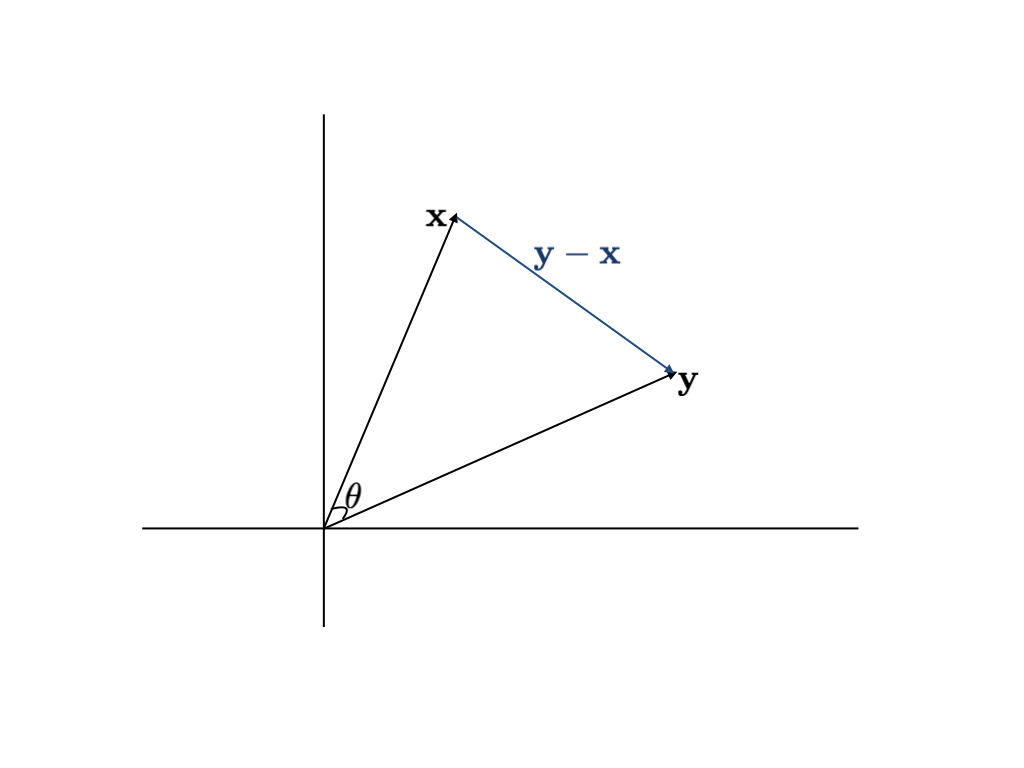
\includegraphics[width=0.7\linewidth]{images/multiple-cos} 

}

\caption{Two vectors in $\mathbb{R}^2$}\label{fig:cosfig}
\end{figure}

\BeginKnitrBlock{proof}
\iffalse{} {Proof. } \fi{}See Figure \ref{fig:cosfig}. We have a triangle. Law of cosines gives that

\[\lVert \mathbf{y} - \mathbf{x} \rVert^2 = \lVert \mathbf{x} \rVert^2 + \lVert \mathbf{y} \rVert^2 -2 \lVert \mathbf{x} \rVert \lVert \mathbf{y} \rVert \cos\theta\]

It follows that

\begin{equation*}
  \begin{split}
    \lVert \mathbf{x} \rVert \lVert \mathbf{y} \rVert \cos\theta & = \frac{1}{2}(\lVert \mathbf{x} \rVert^2 + \lVert \mathbf{y} \rVert^2 - \lVert \mathbf{y} - \mathbf{x} \rVert^2) \\
    & = \frac{1}{2}(\mathbf{x}^T \mathbf{x} + \mathbf{y}^T \mathbf{y} - (\mathbf{y} - \mathbf{x})^T(\mathbf{y} - \mathbf{x})) \\
    & = \mathbf{x}^T\mathbf{y}
  \end{split}
\end{equation*}
\EndKnitrBlock{proof}

This implies the \emph{relationship between sample correlation and the angle}.

\BeginKnitrBlock{theorem}[Sample correlation and the Angle]
\protect\hypertarget{thm:corrangle}{}{\label{thm:corrangle} \iffalse (Sample correlation and the Angle) \fi{} }Let \(\mathbf{X} = (X_1, \ldots, X_n)^T\) and \(\mathbf{Y} = (Y_1, \ldots, Y_n)^T\) be random variables. Then

\[\hat\rho(\mathbf{X}, \mathbf{Y}) = cos \theta\]

where \(\theta\) is the angle between \(\mathbf{X} - \overline{X}\mathbf{1}\) and \(\mathbf{Y} - \overline{Y}\mathbf{1}\).
\EndKnitrBlock{theorem}

\BeginKnitrBlock{proof}
\iffalse{} {Proof. } \fi{}Note that

\[\widehat{Cov}(\mathbf{X}, \mathbf{Y}) = \frac{1}{n - 1} (\mathbf{X} - \overline{X}\mathbf{1})^T(\mathbf{Y} - \overline{Y}\mathbf{1})\]

\[\hat\sigma_{\mathbf{X}} = \sqrt{\frac{1}{n - 1} (\mathbf{X} - \overline{X}\mathbf{1})^T (\mathbf{X} - \overline{X}\mathbf{1})}\]

and

\[\hat\sigma_{\mathbf{Y}} = \sqrt{\frac{1}{n - 1} (\mathbf{Y} - \overline{Y}\mathbf{1})^T (\mathbf{Y} - \overline{Y}\mathbf{1})}\]

and hence it follows that

\begin{equation*}
  \begin{split}
    \hat\rho(\mathbf{X}, \mathbf{Y}) & = \frac{\widehat{Cov}(\mathbf{X}, \mathbf{Y})}{\hat\sigma_{\mathbf{X}}\hat\sigma_{\mathbf{Y}}} \\
    & = \frac{(\mathbf{X} - \overline{X}\mathbf{1})^T(\mathbf{Y} - \overline{Y}\mathbf{1})}{\sqrt{(\mathbf{X} - \overline{X}\mathbf{1})^T (\mathbf{X} - \overline{X}\mathbf{1})}\sqrt{(\mathbf{Y} - \overline{Y}\mathbf{1})^T (\mathbf{Y} - \overline{Y}\mathbf{1})}} \\
    & = \frac{<\mathbf{X} - \overline{X}\mathbf{1}, \mathbf{Y} - \overline{Y}\mathbf{1}>}{\lVert \mathbf{X} - \overline{X}\mathbf{1} \rVert \lVert \mathbf{Y} - \overline{Y}\mathbf{1} \rVert} \\
    & = cos \theta
  \end{split}
\end{equation*}

where \(\theta\) is the angle between \(\mathbf{X} - \overline{X}\mathbf{1}\) and \(\mathbf{Y} - \overline{Y}\mathbf{1}\).
\EndKnitrBlock{proof}

Using this fact, we can finally derive that

\begin{equation}
  \hat\rho(\mathbf{Y}, X\boldsymbol\beta) = \cos\theta
  \label{eq:rsqangle}
\end{equation}

where \(\theta\) is the angle between \(\mathbf{Y} - \overline{Y}\mathbf{1}\) and

\[\beta_1(\mathbf{x}_1 - \overline{x}_1\mathbf{1}) + \cdots \beta_p(\mathbf{x}_p - \overline{x}_p\mathbf{1}) = \mathbb{X}_{A,\perp} \boldsymbol\beta_A \in Col(\mathbb{X}_{A, \perp})\]

\begin{figure}[H]

{\centering 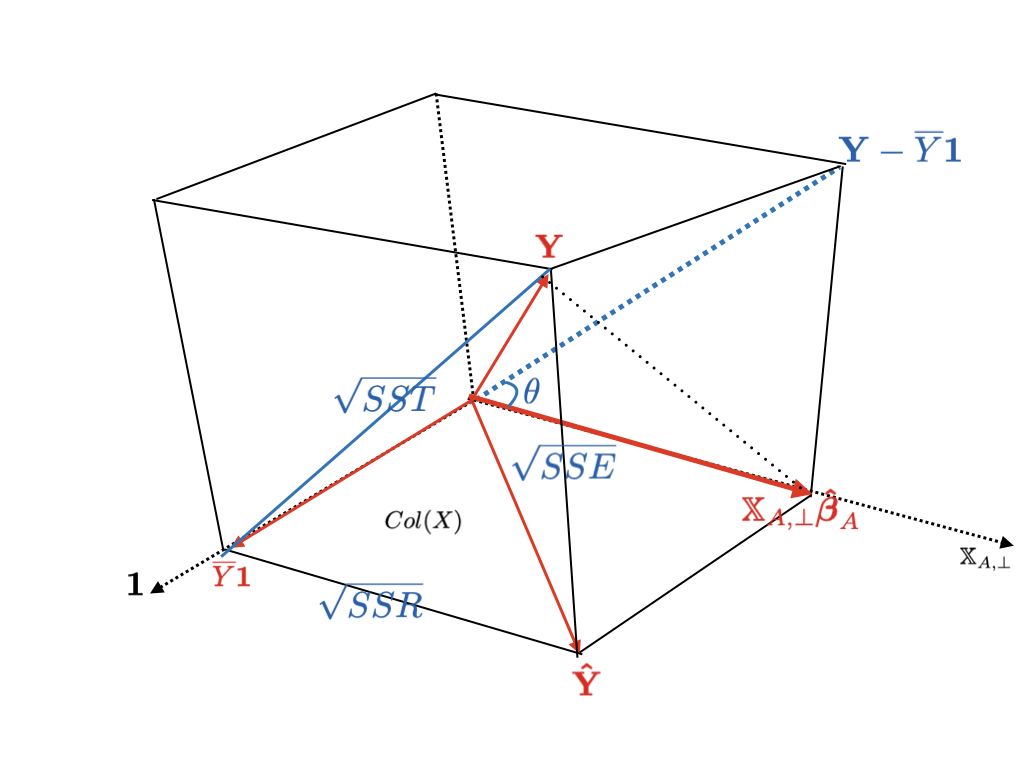
\includegraphics[width=0.7\linewidth]{images/multiple-rsq} 

}

\caption{$R^2$ and Projection}\label{fig:rsqfig}
\end{figure}

See Figure \ref{fig:rsqfig}. \(\theta\) is marked on Figure \ref{fig:mdecomp} setting. In this setting, we know that \(\theta < \frac{\pi}{2}\) is minimized by projection onto \(\mathbb{X}_{A,\perp}\). This means that \(\cos\theta\) is maximized. In other words,

\[R^2 = \frac{SSR}{SST} = (\cos\theta)^2\]

is maximized by the projection of \(\mathbf{Y} - \overline{Y}\mathbf{1}\) onto \(Col(\mathbb{X}_{A, \perp})\). Thus, \(R^2\) can be interpreted as \emph{proportion of variability of \(Y\) that is explained by the set of \(x_j\)s}. It is obvious that \(0 \le R^2 \le 1\).

\(R^2\) becomes larger if a set of \(\mathbb{X}_{A, \perp}\) explains the response well. Is it proper to use this measure as judging \emph{goodness-of-fit}? However, this is not a good measure for model comparison. Model comparison includes different number of predictors. \emph{\(SSE\), however, always decreases when new \(X_j\) is added,} while \(SST = \sum (Y_i - \overline{Y})\) never changes given \(Y\) data. This leads

\[R^2 = 1 - \frac{SSE}{SST}\]

always becomes larger by more predictors. For example,

\[
\begin{cases}
  Y = \beta_0 + \beta_1 X_1 + \epsilon \\
  Y = \beta_0 + \beta_1 X_1 + \beta_1 X_2 + \epsilon
\end{cases}
\]

Whether \(X_2\) additionaly contributes to \(Y\) significantly, \(R^2\) increases and we could judge that second model is better than first one. Hence to use this properly, we need some adjustment. As \(p + 1\) increases, this adjustment should become smaller:

\[\frac{n - 1}{n - p - 1}\]

\BeginKnitrBlock{definition}[Adjusted Rsquared]
\protect\hypertarget{def:ra}{}{\label{def:ra} \iffalse (Adjusted Rsquared) \fi{} }\[R_a^2 := 1 - \frac{SSE / (n - p - 1)}{SST / (n - 1)}\]
\EndKnitrBlock{definition}

\BeginKnitrBlock{remark}[Adjustment]
\iffalse{} {Remark (Adjustment). } \fi{}\[R_a^2 = 1 - \frac{n - 1}{n - p - 1}(1 - R^2)\]
\EndKnitrBlock{remark}

\BeginKnitrBlock{proof}
\iffalse{} {Proof. } \fi{}Note that

\[R^2 = 1 - \frac{SSE}{SST}\]

and hence,

\begin{equation*}
  \begin{split}
    R_a^2 & := 1 - \frac{SSE / (n - p - 1)}{SST / (n - 1)} \\
    & = 1 - \frac{n - 1}{n - p - 1}\bigg(\frac{SSE}{SST}\bigg) \\
    & = 1 - \frac{n - 1}{n - p - 1}(1 - R^2)
  \end{split}
\end{equation*}
\EndKnitrBlock{proof}

So \(R_a^2\) becomes a useful measure for the goodness-of-fit. On the contrary, \emph{it cannot be interpreted as the proportion of total variation in \(Y\) that is explained by \(X_1, \ldots, X_p\).}

\hypertarget{distributions-1}{%
\section{Distributions}\label{distributions-1}}

\hypertarget{individual-regression-coefficients}{%
\subsection{Individual Regression coefficients}\label{individual-regression-coefficients}}

Under Normality,

\[\mathbf{Y} \sim MVN(X\boldsymbol\beta, \sigma^2I)\]

Since \(\boldsymbol{\hat\beta}\) is an unbiased estimator, Proposition \ref{prp:multbmoment} implies that

\begin{equation}
  \boldsymbol{\hat\beta}\sim MVN\bigg( \boldsymbol\beta, \sigma^2(X^TX)^{-1} \bigg)
  \label{eq:hbdist}
\end{equation}

Let \(C \equiv (X^TX)^{-1}\). Then

\[
\begin{bmatrix}
  \hat\beta_0 \\ \hline
  \hat\beta_1 \\ \hline
  \vdots \\ \hline
  \hat\beta_p
\end{bmatrix} \sim MVN\Bigg( \begin{bmatrix}
  \beta_0 \\ \hline
  \beta_1 \\ \hline
  \vdots \\ \hline
  \beta_p
\end{bmatrix}, \sigma^2\begin{bmatrix}
  c_{00} & \cdots & \cdots \\ \hline
  \cdots & c_{11} & \cdots \\ \hline
  \vdots & \vdots & \vdots \\ \hline
  \cdots & \cdots & c_{pp}
\end{bmatrix} \Bigg)
\]

i.e.~Individual coefficient follows

\[\hat\beta_j \sim N(\beta_j, c_{jj}\sigma^2), \quad j = 0, 1, \ldots, p\]

where \(c_{jj}\) is \(j + 1\)th diagonal element of \(C = (X^TX)^{-1}\). Then

\begin{equation}
  \frac{\hat\beta_k - \beta_k}{\sigma\sqrt{c_{kk}}} \sim N(0, 1)
  \label{eq:bejzdist}
\end{equation}

From Proposition \ref{prp:ssdist},

\[\frac{SSE}{\sigma^2} \sim \chi^2(n - p - 1)\]

Since \(\hat\sigma^2 = \frac{SSE}{n - p - 1}\) and \(\hat\beta_k \perp\!\!\!\perp\hat\sigma^2\),

\begin{equation}
  \frac{\hat\beta_k - \beta_k}{\hat\sigma\sqrt{c_{kk}}} = \frac{(\hat\beta_k - \beta_k) / (\sigma\sqrt{c_{kk}}) \sim N(0, 1)}{\sqrt{\frac{SSE}{\sigma^2} / (n - p - 1) \sim \chi^2(n - p - 1)}} \sim t(n - p - 1), \quad k = 0, 1, \ldots, p
  \label{eq:bejtdist}
\end{equation}

\hypertarget{mean-response-1}{%
\subsection{Mean response}\label{mean-response-1}}

Consider prediction at \(\mathbf{z} = (1, z_1, \ldots, z_p)^T\)

Mean response targets

\[\hat\mu_{\mathbf{z}} = \mathbf{z}^T\boldsymbol{\hat\beta}\]

From Equation \eqref{eq:hbdist},

\[\hat\mu_{\mathbf{z}} \sim N(\mathbf{z}^T\boldsymbol\beta, \sigma^2\mathbf{z}^T(X^TX)^{-1}\mathbf{z})\]

Set

\begin{equation}
  C_{\mathbf{z}} := \mathbf{z}^T(X^TX)^{-1}\mathbf{z}
  \label{eq:predse}
\end{equation}

Then by standardization,

\begin{equation}
  \frac{\hat\mu_{\mathbf{z}} - \mu_{\mathbf{z}}}{\sqrt{C_{\mathbf{z}}\sigma^2}} \sim N(0, 1)
  \label{eq:meanreszdist}
\end{equation}

Hence,

\begin{equation}
  \frac{\hat\mu_{\mathbf{z}} - \mu_{\mathbf{z}}}{\sqrt{C_{\mathbf{z}}\hat\sigma^2}} \sim t(n - p - 1)
  \label{eq:meanrestdist}
\end{equation}

\hypertarget{response-1}{%
\subsection{Response}\label{response-1}}

Now we target \(\mathbf{Y}\) at \(\mathbf{z} = (1, z_1, \ldots, z_p)^T\) \emph{out-of-sample}. \(\boldsymbol\epsilon_{\mathbf{z}}\) at this point is independent of the data set.

Consider

\begin{equation}
  \hat{Y}_{\mathbf{z}} - Y_{\mathbf{z}} = \mathbf{z}^T(\boldsymbol{\hat\beta}- \boldsymbol\beta) + \epsilon_{\mathbf{z}}
  \label{eq:prerrz}
\end{equation}

As in Proposition \ref{prp:bepsmvn}, it can be proven that

\[
\begin{bmatrix}
  \boldsymbol{\hat\beta}- \boldsymbol\beta\\
  \epsilon_{\mathbf{z}}
\end{bmatrix} \sim MVN
\]

by showing marginal follows Normal and two are independent. First part - marginal follows normal distribution - has been already shown and assumed. Since these are Normal, it is enough to show covariance is zero.

\begin{equation*}
  \begin{split}
    Cov((\boldsymbol{\hat\beta}- \boldsymbol\beta), \epsilon_{\mathbf{z}}) & = Cov\Big( (X^TX)^{-1}X^T Y, \epsilon_{\mathbf{z}} \Big) \\
    & = (X^TX)^{-1}X^T Cov(Y, \epsilon_{\mathbf{z}}) \\
    & = 0
  \end{split}
\end{equation*}

Hence, the joint distribution

\[
\begin{bmatrix}
  \boldsymbol{\hat\beta}- \boldsymbol\beta\\ \hline
  \epsilon_{\mathbf{z}}
\end{bmatrix} \sim MVN\bigg( \mathbf{0}, \left[\begin{array}{c|c}
  \sigma^2(X^TX)^{-1} & 0 \\ \hline
  0 & \sigma^2
\end{array}\right] \bigg)
\]

From Equation \eqref{eq:prerrz},

\begin{equation*}
  \begin{split}
    \hat{Y}_{\mathbf{z}} - Y_{\mathbf{z}} & = \left[\begin{array}{c|c}
      \mathbf{z}^T & 1
    \end{array}\right] \begin{bmatrix}
      \boldsymbol{\hat\beta}- \boldsymbol\beta\\ \hline
      \epsilon_{\mathbf{z}}
    \end{bmatrix} \\
    & \sim N \Bigg( \mathbf{0}, \left[\begin{array}{c|c}
      \mathbf{z}^T & 1
    \end{array}\right] \left[\begin{array}{c|c}
      \sigma^2(X^TX)^{-1} & 0 \\ \hline
      0 & \sigma^2
    \end{array}\right] \left[\begin{array}{cc}
      \mathbf{z} \\ 1
    \end{array}\right] \Bigg) \\
    & \stackrel{d}{=} N \Big( \mathbf{0}, \sigma^2\mathbf{z}^T(X^TX)^{-1}\mathbf{z} + \sigma^2 \Big)
  \end{split}
\end{equation*}

Using notation from Equation \eqref{eq:predse}, we get

\begin{equation}
  \hat{\mathbf{Y}}_{\mathbf{z}} - \mathbf{Y}_{\mathbf{z}} \sim N\bigg( \mathbf{0}, (C_{\mathbf{z}} + 1)\sigma^2 \bigg)
  \label{eq:resdistn}
\end{equation}

Then standardization gives that

\begin{equation}
  \frac{\hat{Y}_{\mathbf{z}} - Y_{\mathbf{z}}}{\sqrt{(C_{\mathbf{z}} + 1)\sigma^2}} \sim N(0, 1)
  \label{eq:reszdist}
\end{equation}

and hence,

\begin{equation}
  \frac{\hat{Y}_{\mathbf{z}} - Y_{\mathbf{z}}}{\sqrt{(C_{\mathbf{z}} + 1)\hat\sigma^2}} \sim t(n - p - 1)
  \label{eq:restdist}
\end{equation}

Compare Statistic \eqref{eq:restdist} with Statistic \eqref{eq:meanrestdist}. We can see that out-of-sample one has larger standard error by \(\sigma^2\) with same degrees of freedom. This is same as simple regression setting. Error of mean response only comes from \(\boldsymbol{\hat\beta}\). When we predict out-of-sample individual, however, \(Var(\epsilon_{\mathbf{z}})\) is added. Denote that this \(\epsilon_{\mathbf{z}}\) should be independent with given data. Otherwise, we cannot get the distribution as ordinary \citep{Johnson:2013aa}.

\hypertarget{statistical-inference-1}{%
\section{Statistical Inference}\label{statistical-inference-1}}

We have derived basic distributions, so we try to test or build a confidence interval.

\hypertarget{individual-regression-coefficients-1}{%
\subsection{Individual Regression coefficients}\label{individual-regression-coefficients-1}}

From Statistic \eqref{eq:bejtdist}, we can easily make \((1 - \alpha)100\%\) confidence interval \(\hat\theta \pm t_{\frac{\alpha}{2}} SE\) and test statistic.

\BeginKnitrBlock{theorem}[$(1 - \alpha)100\%$ Confidence interval]
\protect\hypertarget{thm:bjci}{}{\label{thm:bjci} \iffalse (\((1 - \alpha)100\%\) Confidence interval) \fi{} }\((1 - \alpha)100\%\) confidence interval for each individual \(\beta_j\) is

\[\bigg[ \hat\beta_j \pm t_{\frac{\alpha}{2}}(n - p - 1) \hat\sigma\sqrt{c_{kk}} \bigg]\]
\EndKnitrBlock{theorem}

In fact, we have already seen the test statistic form.

\BeginKnitrBlock{theorem}[Partial t-test]
\protect\hypertarget{thm:partialt}{}{\label{thm:partialt} \iffalse (Partial t-test) \fi{} }Test \(H_0: \beta_k = \alpha_k \quad \text{vs} \quad H_1: \beta_k \neq \alpha_k\). For given data, partial \(t\)-test computes

\[T_0 = \frac{\hat\beta_k - \alpha_k}{\hat\sigma\sqrt{c_{kk}}} \sim t(n - p - 1)\]

where \((X^TX)^{-1} = (c_{ij})_{0 \le i,j \le p}\)
\EndKnitrBlock{theorem}

As usual test, we reject \(H_0\) when

\[\lvert T_0 \rvert > t_{\frac{\alpha}{2}}(n - p - 1)\]

\begin{figure}[H]

{\centering 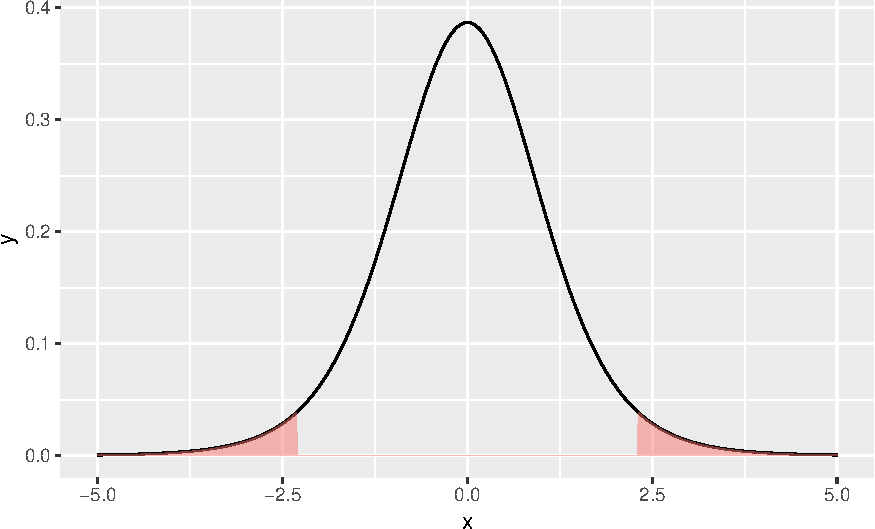
\includegraphics[width=0.7\linewidth]{regression-analysis_files/figure-latex/bjreject-1} 

}

\caption{Rejection region for $\beta_k$}\label{fig:bjreject}
\end{figure}

If we use \texttt{summary()} to \texttt{lm} object, we can get each \(T\) statistic(\texttt{t\ value}), standard error(\texttt{Std.\ Error}), and p-value(\texttt{Pr(\textgreater{}\textbar{}t\textbar{})}). These are the results of partial \(t\)-test.

\begin{Shaded}
\begin{Highlighting}[]
\KeywordTok{summary}\NormalTok{(cem_fit)}
\CommentTok{#> }
\CommentTok{#> Call:}
\CommentTok{#> lm(formula = y ~ ., data = cem)}
\CommentTok{#> }
\CommentTok{#> Residuals:}
\CommentTok{#>    Min     1Q Median     3Q    Max }
\CommentTok{#> -3.175 -1.671  0.251  1.378  3.925 }
\CommentTok{#> }
\CommentTok{#> Coefficients:}
\CommentTok{#>             Estimate Std. Error t value Pr(>|t|)  }
\CommentTok{#> (Intercept)   62.405     70.071    0.89    0.399  }
\CommentTok{#> x1             1.551      0.745    2.08    0.071 .}
\CommentTok{#> x2             0.510      0.724    0.70    0.501  }
\CommentTok{#> x3             0.102      0.755    0.14    0.896  }
\CommentTok{#> x4            -0.144      0.709   -0.20    0.844  }
\CommentTok{#> ---}
\CommentTok{#> Signif. codes:  0 '***' 0.001 '**' 0.01 '*' 0.05 '.' 0.1 ' ' 1}
\CommentTok{#> }
\CommentTok{#> Residual standard error: 2.45 on 8 degrees of freedom}
\CommentTok{#> Multiple R-squared:  0.982,  Adjusted R-squared:  0.974 }
\CommentTok{#> F-statistic:  111 on 4 and 8 DF,  p-value: 4.76e-07}
\end{Highlighting}
\end{Shaded}

If the test is significant, it means that additional contribution of that variable is significant after all other variables are already in the model. This might be understood well with extra sum of squares concept, later.

\hypertarget{prediction-interval-1}{%
\subsection{Prediction interval}\label{prediction-interval-1}}

Consider prediction at \(\mathbf{z} = (1, z_1, \ldots, z_p)^T\). Write

\[C_{\mathbf{z}} := \mathbf{z}^T(X^TX)^{-1}\mathbf{z}\]

\BeginKnitrBlock{theorem}[Prediction or Confidence interval for mean response]
\protect\hypertarget{thm:meanresci}{}{\label{thm:meanresci} \iffalse (Prediction or Confidence interval for mean response) \fi{} }\((1 - \alpha)100\%\) prediction interval for \(\mu_{\mathbf{z}}\) is

\[\bigg[ \hat\mu_{\mathbf{z}} \pm t_{\frac{\alpha}{2}}(n - p - 1)\sqrt{C_{\mathbf{z}}\hat\sigma^2} \bigg]\]
\EndKnitrBlock{theorem}

\BeginKnitrBlock{theorem}[Out-of-sample prediction interval]
\protect\hypertarget{thm:predresci}{}{\label{thm:predresci} \iffalse (Out-of-sample prediction interval) \fi{} }\((1 - \alpha)100\%\) prediction interval for \(Y_{\mathbf{z}}\) is

\[\bigg[ \hat{Y}_{\mathbf{z}} \pm t_{\frac{\alpha}{2}}(n - p - 1)\sqrt{(C_{\mathbf{z}} + 1)\hat\sigma^2} \bigg]\]
\EndKnitrBlock{theorem}

See standard error part of Theorem \ref{thm:meanresci} and Theorem \ref{thm:predresci}. As mentioned, Out of sample prediction interval \emph{always has larger standard error.} This leads to wider interval.

\hypertarget{regression-coefficient-vector}{%
\subsection{Regression coefficient vector}\label{regression-coefficient-vector}}

Now we consider the coefficients simultaneously. For example, \(\boldsymbol\beta= (\beta_0, \beta_1, \ldots, \beta_p)^T\).

Note that

\[\boldsymbol{\hat\beta}- \boldsymbol\beta\sim MVN(\mathbf{0}, \sigma^2(X^TX)^{-1})\]

Then standardization gives

\[\mathbf{Z} \equiv \frac{(X^TX)^{\frac{1}{2}}}{\sigma}(\boldsymbol{\hat\beta}- \boldsymbol\beta) \sim MVN(\mathbf{0}, I)\]

It follows that

\[\mathbf{Z}^T\mathbf{Z} = \frac{(\boldsymbol{\hat\beta}- \boldsymbol\beta)^T X^TX (\boldsymbol{\hat\beta}- \boldsymbol\beta)}{\sigma^2} \sim \chi^2(p + 1)\]

Since \(\frac{SSE}{\sigma^2} \sim \chi^2(n - p - 1)\) and \(\hat\sigma^2 = MSE\),

\begin{equation}
  \begin{split}
    \frac{(\boldsymbol{\hat\beta}- \boldsymbol\beta)^T X^TX (\boldsymbol{\hat\beta}- \boldsymbol\beta)}{\hat\sigma^2 (p + 1)} & = \frac{(X\boldsymbol{\hat\beta}- X\boldsymbol\beta)^T(X\boldsymbol{\hat\beta}- X\boldsymbol\beta)}{MSE} \\
    & = \frac{SSR / (p + 1)}{SSE / (n - p - 1)} \\
    & \sim F(p + 1, n - p - 1, \delta)
  \end{split}
  \label{eq:bvecdist}
\end{equation}

where \(\delta = \frac{\boldsymbol\beta^TX^T(I - \Pi_{\mathbf{1}})X\boldsymbol\beta}{\sigma^2}\).

\BeginKnitrBlock{corollary}[F-test]
\protect\hypertarget{cor:bvech0}{}{\label{cor:bvech0} \iffalse (F-test) \fi{} }Test \(H_0: \boldsymbol\beta= \mathbf{0} \quad \text{vs} \quad H_1: \boldsymbol\beta\neq \mathbf{0}\). For given data, \(F\)-test computes

\[\frac{(\boldsymbol{\hat\beta}- \boldsymbol\beta)^T X^TX (\boldsymbol{\hat\beta}- \boldsymbol\beta)}{\hat\sigma^2 (p + 1)} = \frac{SSR / (p + 1)}{MSE} \stackrel{H_0}{\sim}F(p + 1, n - p - 1)\]
\EndKnitrBlock{corollary}

From the first part, we can get the confidence region for \(\boldsymbol\beta\).

\BeginKnitrBlock{theorem}[Confidence region]
\protect\hypertarget{thm:bveccr}{}{\label{thm:bveccr} \iffalse (Confidence region) \fi{} }\((1 - \alpha)100\%\) confidence interval for \(\boldsymbol\beta= (\beta_0, \beta_1, \ldots, \beta_p)^T\) is

\[\Big\{ \boldsymbol\beta: (\boldsymbol{\hat\beta}- \boldsymbol\beta)^T X^TX (\boldsymbol{\hat\beta}- \boldsymbol\beta) \le (p + 1)\hat\sigma^2 F_{1 - \alpha}(p + 1, n - p - 1) \Big\}\]
\EndKnitrBlock{theorem}

\BeginKnitrBlock{remark}
\iffalse{} {Remark. } \fi{}The confidence region for the vector \(\boldsymbol\beta\) is the ellipsoid that is centered at \(\boldsymbol{\hat\beta}\). Eigenvectors and eigenvalues of \(X^TX\) determines its orientation and size, respectively. See \citet{Johnson:2013aa} for details.
\EndKnitrBlock{remark}

\texttt{ellipse::ellipse()} has method for \texttt{lm} object. So if you provides the regression object, it will give ellipsoid coordinate as \texttt{matrix}. However, this function only supports two variables. By specifying \texttt{which} argument, you can select which variable to get coordinates. By default, first two variables \texttt{c(1,\ 2)}.

\begin{Shaded}
\begin{Highlighting}[]
\NormalTok{ellipse}\OperatorTok{::}\KeywordTok{ellipse}\NormalTok{(cem_fit) }\OperatorTok\StringTok{ }
\StringTok{  }\KeywordTok{tbl_df}\NormalTok{() }\OperatorTok\StringTok{ }\CommentTok{# change to data frame}
\StringTok{  }\KeywordTok{ggplot}\NormalTok{(}\KeywordTok{aes}\NormalTok{(}\DataTypeTok{x =} \StringTok{`}\DataTypeTok{(Intercept)}\StringTok{`}\NormalTok{, }\DataTypeTok{y =}\NormalTok{ x1)) }\OperatorTok{+}
\StringTok{  }\KeywordTok{geom_path}\NormalTok{()}
\end{Highlighting}
\end{Shaded}

\begin{figure}[H]

{\centering 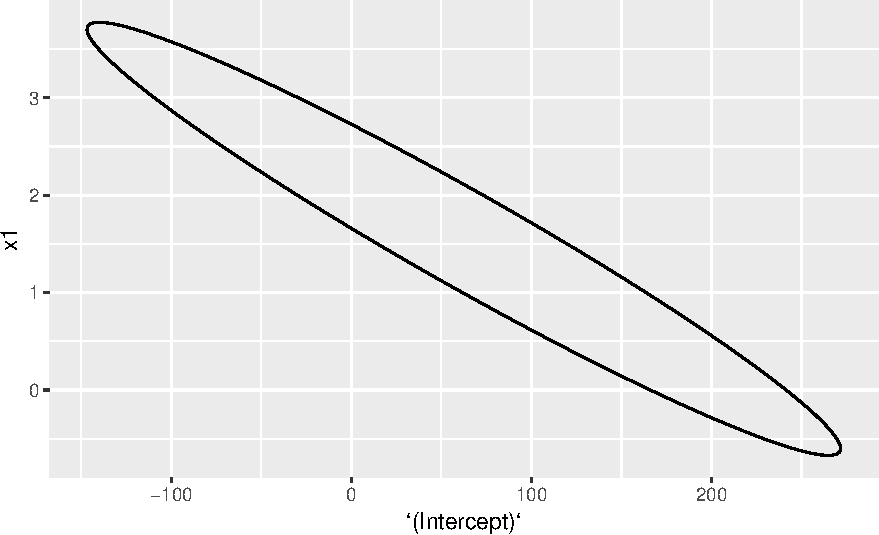
\includegraphics[width=0.7\linewidth]{regression-analysis_files/figure-latex/ellip-1} 

}

\caption{Confidence region for $(\beta_0, \beta_1)$}\label{fig:ellip}
\end{figure}

Look again corollary \ref{cor:bvech0}. Compare this to ANOVA. Something is different. When testing significance in ANOVA, degrees of freedom of \(SSR\) was \(p\). Because when testing regression relation, we only need \(\beta_1\) to \(\beta_p\), i.e.~\(p\) parameters. How can we do this here?

\hypertarget{regression-coefficient-vector-boldsymbolbeta_a}{%
\subsection{\texorpdfstring{Regression coefficient vector \(\boldsymbol\beta_A\)}{Regression coefficient vector \textbackslash boldsymbol\textbackslash beta\_A}}\label{regression-coefficient-vector-boldsymbolbeta_a}}

Consider \(\boldsymbol\beta_A = (\beta_1, \ldots, \beta_p)^T\). In fact, these tell us significance of variables. We can use \(\mathbb{X}_{A, \perp}\) defined before. From Equation \eqref{eq:orthbeta},

\[\boldsymbol{\hat\beta}_A = (\mathbb{X}_{A,\perp}^T\mathbb{X}_{A,\perp})^{-1}\mathbb{X}_{A,\perp}^T\mathbf{Y}\]

The reason using \(\mathbb{X}_{A, \perp}\) is to decomposing the space orthogonally.

\[
\boldsymbol{\hat\beta}- \boldsymbol\beta= \begin{bmatrix}
  \hat\beta_0 - \beta_0 \\ \hline
  \boldsymbol{\hat\beta}_A - \boldsymbol\beta_A
\end{bmatrix} \sim MVN\Bigg( \begin{bmatrix}
  0 \\ \hline
  \mathbf{0}
\end{bmatrix}, \sigma^2 (X^T X)^{-1} \bigg)
\]

with

\[Var(\boldsymbol{\hat\beta}_A - \boldsymbol\beta_A) = \sigma^2 (\mathbb{X}_{A, \perp}^T\mathbb{X}_{A, \perp})^{-1}\]

\BeginKnitrBlock{theorem}[Confidence region]
\protect\hypertarget{thm:bacr}{}{\label{thm:bacr} \iffalse (Confidence region) \fi{} }\((1 - \alpha)100\%\) confidence interval for \(\boldsymbol\beta_A = (\beta_1, \ldots, \beta_p)^T\) is

\[\Big\{ \boldsymbol\beta_A : (\boldsymbol{\hat\beta}_A - \boldsymbol\beta_A)^T \mathbb{X}_{A, \perp}^T\mathbb{X}_{A, \perp} (\boldsymbol{\hat\beta}_A - \boldsymbol\beta_A) \le p \hat\sigma^2 F_{\alpha}(p, n - p - 1) \Big\}\]

where \(\boldsymbol{\hat\beta}_A = (\mathbb{X}_{A,\perp}^T\mathbb{X}_{A,\perp})^{-1}\mathbb{X}_{A,\perp}^T\mathbf{Y}\)
\EndKnitrBlock{theorem}

This tests the same hypothesis as ANOVA for significance.

\BeginKnitrBlock{remark}
\iffalse{} {Remark. } \fi{}As for \(X\), the confidence region for the vector \(\boldsymbol\beta_A\) is the ellipsoid that is centered at \(\boldsymbol{\hat\beta}_A\). Eigenvectors and eigenvalues of \(\mathbb{X}_{A, \perp}^T\mathbb{X}_{A, \perp}\) determines its orientation and size, respectively.
\EndKnitrBlock{remark}

\hypertarget{nested-models}{%
\section{Nested Models}\label{nested-models}}

We have seen \(t\)-test and \(F\)-test testing \(\beta_j = 0\) and \(\beta_1 = \cdots = \beta_p = 0\), respectively. Here, we generalize the hypothesis in terms of \emph{nested model}. Consider several types of hypothesis.

\BeginKnitrBlock{example}[Examples of three types of hypothesis]
\protect\hypertarget{exm:ftestex}{}{\label{exm:ftestex} \iffalse (Examples of three types of hypothesis) \fi{} }We can test if every coefficient is zero or some coefficient is zero, or just test if coefficients are same not specific value.

\begin{enumerate}
  \item $H_0: \beta_1 = \cdots = \beta_p = 0$
  \item $H_0: \beta_{p - 1} = \beta_p = 0$
  \item $H_0: \beta_{p - 1} = \beta_p$
\end{enumerate}
\EndKnitrBlock{example}

What is the unified approach to these kind of test?

\hypertarget{full-model-and-reduced-model}{%
\subsection{Full model and reduced model}\label{full-model-and-reduced-model}}

To test some forms of \(H_0\), consider two nested model.

\BeginKnitrBlock{definition}[Nested models]
\protect\hypertarget{def:fmrm}{}{\label{def:fmrm} \iffalse (Nested models) \fi{} }We name nested models for the test as follow.

\begin{enumerate}
  \item \textbf{\textit{Full model}} (FM) represents the basic starting model
  \item \textbf{\textit{Reduced model}} (RM) represents the null model under $H_0$
\end{enumerate}
\EndKnitrBlock{definition}

In Example \ref{exm:ftestex}, the basic starting model, i.e.~FM is

\[Y_i = \beta_0 + \beta_1 x_{i1} + \cdots + \beta_p x_{ip} + \epsilon_i, \quad \epsilon_i \stackrel{iid}{\sim}N(0, \sigma^2)\]

See the second case.

\[H_0: \beta_{p - 1} = \beta_p = 0 \qquad \text{vs} \qquad H_1: \beta_{p - 1} \neq 0 \:\text{or}\: \beta_p \neq 0\]

This is equivalent to choosing a model between

\[
\begin{cases}
  FM: Y_i = \beta_0 + \beta_1 x_{i1} + \cdots + \beta_p x_{ip} + \epsilon_i \\
  RM: Y_i = \beta_0 + \beta_1 x_{i1} + \cdots + \beta_{p - 2}x_{i,p-2} + \epsilon_i
\end{cases}
\]

Let us define \(SSR\) and \(SSE\) for each model.

\BeginKnitrBlock{definition}[SS of nested models]
\protect\hypertarget{def:ssfmrm}{}{\label{def:ssfmrm} \iffalse (SS of nested models) \fi{} }For each full model and reduced model, compute \(SSR\) and \(SSE\).

\begin{enumerate}
  \item $SSR(FM)$ regression sum of squares after fitting the FM
  \item $SSE(FM)$ error sum of squares after fitting the FM
  \item $SSR(RM)$ regression sum of squares after fitting the RM
  \item $SSR(RM)$ error sum of squares after fitting the RM
\end{enumerate}
\EndKnitrBlock{definition}

By construction, \(SST = \sum\limits_{i = 1}^n(Y_i - \overline{Y})^2\) does not depend on model. This measures variability when no predictor is used. It jus the variation of a response itself. So it becomes consistent with given data.

\BeginKnitrBlock{remark}
\iffalse{} {Remark. } \fi{}\[SST = SSR(FM) + SSE(FM) = SSR(RM) + SSE(RM)\]

and hence

\[SSE(RM) - SSE(FM) = SSR(FM) - SSR(RM)\]
\EndKnitrBlock{remark}

\(SSE\) indicates a variation that cannot be explained by the model. \(SSR\) represents a variation explained by the model. We can compare each between the two model. If \(SSE(RM) - SSE(FM) = SSR(FM) - SSR(RM)\) is large, then we can think that the full model is explaining given data better than reduced model. Or, \(SSE\) says that full model can explain some parts that reduced model have failed to explained. In terms of \(H_0: RM \:\text{vs}\: H_1: FM\), it can be said that it is a strong evidene supporting FM against RM. In turn, we conclude that \(H_1: \beta_{p - 1} \neq 0 \:\text{or}\: \beta_p \neq 0\) from our first hypothesis set.

\BeginKnitrBlock{conjecture}
\protect\hypertarget{cnj:fmrmdist}{}{\label{cnj:fmrmdist} }\[SSR(FM) - SSR(RM) > c \Leftrightarrow \text{reject}\: H_0\]
\EndKnitrBlock{conjecture}

We can test any hypothesis using RM-FM pair as in Conjecture \ref{cnj:fmrmdist}. The question is

\begin{enumerate}
\def\labelenumi{\arabic{enumi}.}
\tightlist
\item
  What is the distribution of \(SSR(FM) - SSR(RM)\)?
\item
  Then what is \(c\)?
\end{enumerate}

Define two design matrices to build full model and reduced model.

\[
Z_1 := \begin{bmatrix}
  1 & x_{11} & \cdots & x_{1, p - 2} \\
  1 & x_{21} & \cdots & x_{2, p - 2} \\
  \vdots & \vdots & \vdots & \vdots \\
  1 & x_{n1} & \cdots & x_{n,p - 2}
\end{bmatrix}, \quad \text{and} \qquad Z_2 := \begin{bmatrix}
  x_{1, p - 1} & x_{1p} \\
  x_{2, p - 1} & x_{2p} \\
  \vdots & \vdots \\
  x_{n, p - 1} & x_{np}
\end{bmatrix}
\]

\(Z_1\) is a design matrix of reduced model, while \(Z_2\) consists of column vector that was not in \(Z_2\), i.e.~which were specified in \(H_0\). It is intended to make

\[
X^{\ast} = \begin{bmatrix}
  Z_1 \mid Z_2
\end{bmatrix} \in \mathbb{R}^{n \times (p + 1)}
\]

where \(X^{\ast}\) can have different column order with original \(X\). It follows that

\[
\begin{cases}
  FM: \mathbf{Y} = X\boldsymbol\beta_F + \E \\
  RM: \mathbf{Y} = Z_1 \boldsymbol\beta_R + \E
\end{cases}
\]

where \(\boldsymbol\beta_F = (\beta_0, \ldots, \beta_p)^T\) and \(\boldsymbol\beta_R = (\beta_0, \beta_1, \ldots, \beta_{p - 2})^T\). Thus,

\begin{equation}
  \begin{cases}
    SSR(FM) = \mathbf{Y}^T (\Pi_X - \Pi_{\mathbf{1}}) \mathbf{Y} \\
    SSR(RM) = \mathbf{Y}^T (\Pi_{Z_1} - \Pi_{\mathbf{1}}) \mathbf{Y}
  \end{cases}
  \label{eq:ssrfmrm}
\end{equation}

and so

\begin{equation}
  \begin{split}
    SSR(FM) - SSR(RM) & = \mathbf{Y}^T (\Pi_X - \Pi_{\mathbf{1}} - \Pi_{Z_1} + \Pi_{\mathbf{1}}) \mathbf{Y} \\
    & = \mathbf{Y}^T (\Pi_X - \Pi_{Z_1}) \mathbf{Y}
  \end{split}
  \label{eq:fmrmstat}
\end{equation}

\BeginKnitrBlock{lemma}
\protect\hypertarget{lem:ssrfmlem}{}{\label{lem:ssrfmlem} }\(SSR(FM) - SSR(RM)\) satisfies following properties.

\begin{enumerate}
  \item $\Pi_X - \Pi_{Z_1}$ is symmetric and idempotent
  \item $tr(\Pi_X - \Pi_{Z_1}) = (p + 1) - \text{number of parameters in reduced model}$
  \item $SSR(FM) - SSR(RM) \perp\!\!\!\perp SSE(FM)$
\end{enumerate}
\EndKnitrBlock{lemma}

\BeginKnitrBlock{proof}
\iffalse{} {Proof. } \fi{}Propery of prjection implies that

\[\Pi_X \Pi_{Z_1} = \Pi_{Z_1}\]

Note that

\[SSE(FM) = \mathbf{Y}^T (I - \Pi_X) \mathbf{Y}\]

Then

\[(\Pi_X - \Pi_{Z_1})(I - \Pi_X) = 0\]

Hence, \(SSR(FM) - SSR(RM) \perp\!\!\!\perp SSE(FM)\)
\EndKnitrBlock{proof}

Go back to our Example \ref{exm:ftestex}. Denote that \(\Pi_X - \Pi_{Z_1}\) implies that \(R_{p - 1}^2 > R_{p - 2}^2\). It is easy to get

\[tr(\Pi_X - \Pi_{Z_1}) = (p + 1) - (p - 1) = 2\]

Then

\begin{equation}
  \frac{SSR(FM) - SSR(RM)}{\sigma^2} \stackrel{H_0}{\sim}\chi^2(2)
  \label{eq:ssrfmnull}
\end{equation}

From Proposition \ref{prp:ssdist}

\[\frac{SSE(FM)}{\sigma^2} \stackrel{H_0}{\sim}\chi^2(n - p - 1)\]

Since \(SSR(FM) - SSR(RM) \perp\!\!\!\perp SSE(FM)\),

\begin{equation}
  \begin{split}
    \frac{(SSR(FM) - SSR(RM)) / 2}{SSE(FM) / (n - p - 1)} & = \frac{\frac{SSR(FM) - SSR(RM)}{\sigma^2} / 2}{\frac{SSE(FM)}{\sigma^2} / (n - p - 1)} \\
    & \stackrel{H_0}{\sim}F(2, n - p - 1)
  \end{split}
  \label{eq:ssrfmstat}
\end{equation}

Hence, for our

\[H_0: \beta_{p - 1} = \beta_p = 0 \qquad \text{vs} \qquad H_1: \beta_{p - 1} \neq 0 \:\text{or}\: \beta_p \neq 0\]

reject \(H_0\) if \(\frac{(SSR(FM) - SSR(RM)) / 2}{SSE(FM) / (n - p - 1)} > F_{\alpha}(2, n - p - 1)\).

See the numerator part \(SSR(FM) - SSR(RM)\) we have been explored. This can be also written as

\[SSR(X_1, \ldots, X_p) - SSR(X_1, \ldots, X_{p - 2})\]

and this is called \emph{extra sum of squares}.

\hypertarget{extra-sum-of-squares}{%
\subsection{Extra sum of squares}\label{extra-sum-of-squares}}

\BeginKnitrBlock{definition}[Extra sum of squares]
\protect\hypertarget{def:ess}{}{\label{def:ess} \iffalse (Extra sum of squares) \fi{} }Extra sum of squares measures the amount of the additional contribution of variables added after the variables that were already considered. For example,

\[SSR(X_2 \mid X_1) := SSR(X_1, X_2) - SSR(X_1)\]

This measures marginal contribution of \(X_2\) after \(X_1\) is considred. Here, the contribution means marginal increase of \(SSR\). Equivalently, marginal decrease of \(SSE\).
\EndKnitrBlock{definition}

\begin{figure}[H]

{\centering 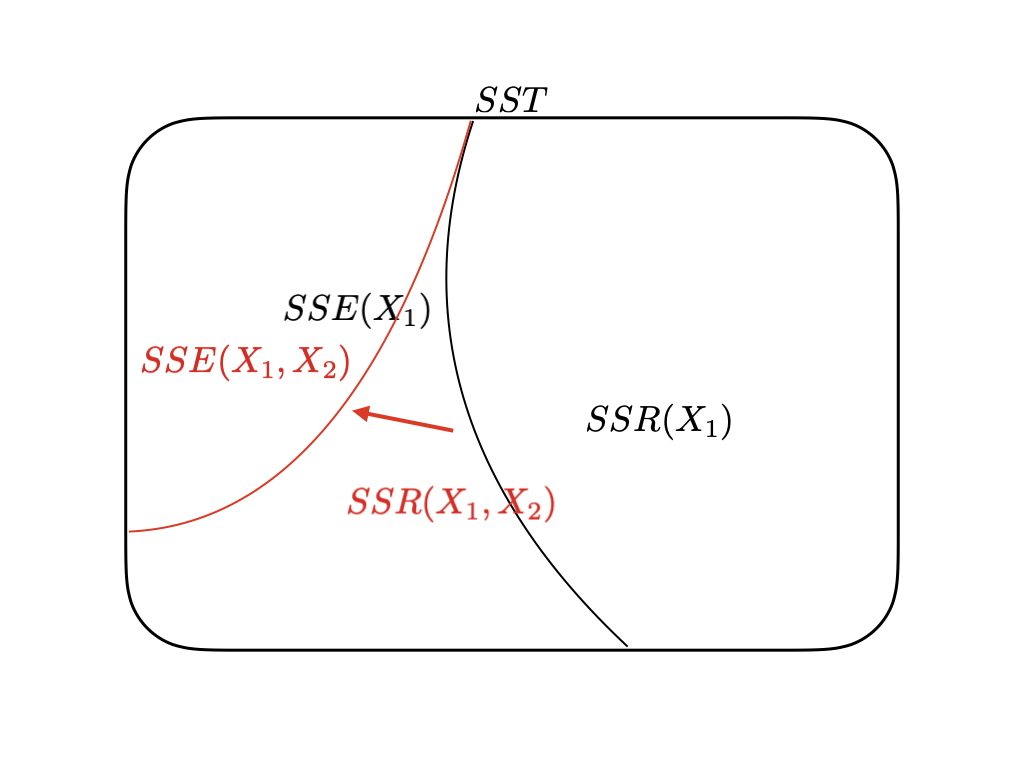
\includegraphics[width=0.7\linewidth]{images/multiple-extrass} 

}

\caption{Extra sum of squares - SSR increases and SSE decreases}\label{fig:essfig}
\end{figure}

Similarly,

\[SSR(X_3, X_4 \mid X_1, X_2) := SSR(X_1, X_2, X_3, X_4) - SSR(X_1, X_2)\]

measures of \(X_3\) and \(X_4\) after \(X_1\) and \(X_2\) are already in the model.

\(SST\) does not change given data. By adding some variables, \(SSR\) increases or \(SSE\) decreases. \emph{We interpret this change as additional contribution of those variables}. If it is large enough, they are significant. Using this idea, we might test any kind of sets of coefficients. Partial \(F\)-test and sequential \(F\)-test are typical forms that we can think of and useful.

\hypertarget{partial-f-test}{%
\subsection{Partial F test}\label{partial-f-test}}

Focus on marginal contribution given that every other predictor is already in the model.

\BeginKnitrBlock{definition}[Partial sum of squares]
\protect\hypertarget{def:pss}{}{\label{def:pss} \iffalse (Partial sum of squares) \fi{} }Partial SS or Type III Sum of squares are following.

\begin{itemize}
  \item $SSR(X_1 \mid X_2, \ldots, X_p)$
  \item $SSR(X_2 \mid X_1, X_3, \ldots, X_p)$
  \item $SSR(X_3 \mid X_1, X_2, X_4, \ldots, X_p)$
  \item $\vdots$
  \item $SSR(X_p \mid X_1, \ldots, X_{p - 1})$
\end{itemize}
\EndKnitrBlock{definition}

\BeginKnitrBlock{remark}
\iffalse{} {Remark. } \fi{}Partial SS satisties following properties.

\begin{enumerate}
  \item $SSR(X_1 \mid X_2, \ldots X_p) + \cdots + SSR(X_p \mid X_1, \ldots, X_{p - 1}) \neq SSR(X_1, \ldots, X_p)$
  \item Partial SS (Type III SS) represents the additional contribution of each predictor after the other predictor variables are considred.
\end{enumerate}
\EndKnitrBlock{remark}

Partial \(F\)-test aims at testing single coefficient.

\[H_0: \beta_j = 0 \qquad \text{vs} \qquad H_1 : \beta_j \neq 0\]

How to make test statistic is same as previous session: using full model and reduced model. Here, one with and without \(\beta_j\).

\begin{equation}
  F_0 = \frac{SSR(X_j \mid X_1, \ldots, X_{j - 1}, X_{j + 1}, \ldots, X_p) / 1}{SSE / (n - p - 1)} \stackrel{H_0}{\sim}F(1, n - p - 1)
  \label{eq:partialstat}
\end{equation}

Hence, reject \(H_0\) if \(F_0 > F_{\alpha}(1, n - p - 1)\). Since the first degrees of freedom is \(1\), we have

\[F_0 = \bigg( \frac{\hat\beta_j}{\widehat{SE}(\hat\beta_j)} \bigg)^2 = T_0^2\]

\BeginKnitrBlock{remark}
\iffalse{} {Remark. } \fi{}Partial \(F\)-test is equivalent to partial \(t\)-test. Both tests the additional contribution of \(X_j\) after the other variables are already considered, not individual significance.
\EndKnitrBlock{remark}

\hypertarget{sequential-f-test}{%
\subsection{Sequential F test}\label{sequential-f-test}}

This sequential \(F\)-test adds variable sequentially.

\BeginKnitrBlock{definition}[Sequential sum of squares]
\protect\hypertarget{def:seqs}{}{\label{def:seqs} \iffalse (Sequential sum of squares) \fi{} }Sequential SS or Type I Sum of squares are following.

\begin{enumerate}
  \item $SSR(X_1)$
  \item $SSR(X_2 \mid X_1)$
  \item $SSR(X_3 \mid X_1, X_2)$
  \item $\vdots$
  \item $SSR(X_p \mid X_1, \ldots, X_{p - 1})$
\end{enumerate}
\EndKnitrBlock{definition}

\BeginKnitrBlock{remark}
\iffalse{} {Remark. } \fi{}Sequential SS satisfies following properties.

\begin{enumerate}
  \item $SSR(X_1) + SSR(X_2 \mid X_1) + \cdots + SSR(X_p \mid X_1, \ldots, X_{p - 1}) = SSR(X_1, \ldots, X_p)$
  \item Sequential SS is useful when we consider nested model. That is, when we know that $X_1$ is the most important, $X_2$ is the second important, and so on.
\end{enumerate}
\EndKnitrBlock{remark}

Following Definition \ref{def:seqs}, start from intercept-only model.

\begin{algorithm}[H] \label{alg:algseq}
  \SetAlgoLined
  \SetKwInOut{Input}{input}
  \SetKwInOut{Output}{output}
  $j \leftarrow 1$\;
  \Repeat{accept $H_0$}{
     $\begin{cases} FM : Y_i = \beta_0 + \cdots + \beta_j x_{1j} + \epsilon_i \\ RM : Y_i = \beta_0 + \ldots + \beta_{j - 1}x_{1, j - 1} + \epsilon_i \end{cases}$\;
    $H_0: \beta_j = 0 (RM) \quad \text{vs} \quad H_1: \beta_j \neq 0 (FM)$\;
    $F_0 = \frac{SSR(X_j \mid X_1, \ldots, X_{j - 1}) / 1}{SSE(X_1, \ldots, X_j) / (n - j - 1)}$\;
    reject $H_0$ if $F_0 > F_{1 - \alpha}(1, n - j - 3)$\;
    $j \leftarrow j + 1$\;
  }
  \Output{accepted model, i.e. final $RM$}
  \caption{Sequential F Test from beginning}
\end{algorithm}

Algorithm \(\ref{alg:algseq}\) shows the logic how to add a variable sequentially. It continues until rejecting \(H_0\). In general form, we can test

\[H_0: \beta_{q + 1} = \beta_{q + 2} = \cdots = \beta_p = 0 \qquad \text{vs} \qquad H_1: \text{not}\: H_0\]

Here, reject \(H_0\) if

\begin{equation}
  \frac{\Big(SSR(X_1, \ldots, X_p) - SSR(X_1, \ldots, X_q)\Big) / (p - q)}{SSE(X_1, \ldots, X_p) / (n - p - 1)} > F_{\alpha}(p - q, n - p - 1)
  \label{eq:seqgen}
\end{equation}

This form of test might be useful when see the significance of categorical predictor. In regression model, quantative predictor is modeled as multiple dummy variables. In this case, we have to see these coefficients all at once and sequential \(F\)-test form might be helpful \citep{Hastie:2013aa}.

\hypertarget{general-linear-hypothesis}{%
\subsection{General linear hypothesis}\label{general-linear-hypothesis}}

See Example \ref{exm:ftestex} again. The third one, \(H_0: \beta_{p - 1} = \beta_p\) can be also tested using \(F\)-test by changing model representation.

\[H_0: \beta_{p - 1} = \beta_p = \alpha \quad \forall \alpha\]

Then null model can be set as

\[Y_i = \beta_0 + \beta_1 x_{i1} + \cdots + \beta_{p - 2} x_{i, p - 2} + \alpha(x_{i, p - 1} + x_{ip}) + \epsilon_i\]

However, there is a more general test procedure: linear combination. For instance, \(\beta_{p - 1} = \beta_p\) can be represented as

\[\beta_{p - 1} - \beta_p = 0 \Leftrightarrow (0, \ldots, 0, 1, -1)^T \boldsymbol\beta= 0\]

Now we analyze this form of hypothesis.

\[H_0: C \boldsymbol\beta= \mathbf{d} \qquad \text{vs} \qquad H_1: C \boldsymbol\beta\neq \mathbf{d}\]

Since \(\hat{\boldsymbol\beta} \sim MVN(\boldsymbol\beta, \sigma^2(X^TX)^{-1})\),

\[C\hat{\boldsymbol\beta} \sim MVN(C \boldsymbol\beta, \sigma^2 C(X^TX)^{-1}C^T)\]

and under \(H_0: C\boldsymbol\beta= \mathbf{d}\),

\[C\hat{\boldsymbol\beta} \stackrel{H_0}{\sim}MVN(\mathbf{d}, \sigma^2 C(X^TX)^{-1}C^T)\]

Set

\[\mathbf{Z} \equiv \frac{1}{\sigma} (C(X^TX)^{-1}C^T)^{-\frac{1}{2}} (C \hat{\boldsymbol\beta} - \mathbf{d}) \stackrel{H_0}{\sim}MVN(\mathbf{0}, I)\]

It follows that

\[\mathbf{Z}^T\mathbf{Z} = \frac{1}{\sigma^2}(C\hat{\boldsymbol\beta} - \mathbf{d})^T(C(X^TX)^{-1}C^T)^{-1}(C\hat{\boldsymbol\beta} - \mathbf{d}) \stackrel{H_0}{\sim}\chi^2(q = rank(C))\]

Since \(SSE \perp\!\!\!\perp\boldsymbol{\hat\beta}\) (See Proposition \ref{prp:ssdist}),

\begin{equation}
  \begin{split}
    \frac{\frac{(C\hat{\boldsymbol\beta} - \mathbf{d})^T(C(X^TX)^{-1}C^T)^{-1}(C\hat{\boldsymbol\beta} - \mathbf{d})}{\sigma^2} / q}{\frac{SSE}{\sigma^2} / (n - p - 1)} & = \frac{(C\hat{\boldsymbol\beta} - \mathbf{d})^T(C(X^TX)^{-1}C^T)^{-1}(C\hat{\boldsymbol\beta} - \mathbf{d}) / q}{\hat\sigma^2} \\
    & \stackrel{H_0}{\sim}F(q, n - p - 1)
  \end{split}
  \label{eq:lincombtest}
\end{equation}

\hypertarget{extra-ss-in-r}{%
\subsection{\texorpdfstring{Extra SS in \texttt{R}}{Extra SS in R}}\label{extra-ss-in-r}}

\texttt{anova.lm()} gives extra sum of squres by default, which is \emph{sequential sum of squares}, i.e.~type I SS.

\begin{Shaded}
\begin{Highlighting}[]
\KeywordTok{anova}\NormalTok{(cem_fit)}
\CommentTok{#> Analysis of Variance Table}
\CommentTok{#> }
\CommentTok{#> Response: y}
\CommentTok{#>           Df Sum Sq Mean Sq F value  Pr(>F)    }
\CommentTok{#> x1         1   1450    1450  242.37 2.9e-07 ***}
\CommentTok{#> x2         1   1208    1208  201.87 5.9e-07 ***}
\CommentTok{#> x3         1     10      10    1.64    0.24    }
\CommentTok{#> x4         1      0       0    0.04    0.84    }
\CommentTok{#> Residuals  8     48       6                    }
\CommentTok{#> ---}
\CommentTok{#> Signif. codes:  0 '***' 0.001 '**' 0.01 '*' 0.05 '.' 0.1 ' ' 1}
\end{Highlighting}
\end{Shaded}

If we change the order,

\begin{Shaded}
\begin{Highlighting}[]
\KeywordTok{anova}\NormalTok{(}\KeywordTok{lm}\NormalTok{(y }\OperatorTok{~}\StringTok{ }\NormalTok{x2 }\OperatorTok{+}\StringTok{ }\NormalTok{x1 }\OperatorTok{+}\StringTok{ }\NormalTok{x3 }\OperatorTok{+}\StringTok{ }\NormalTok{x4, }\DataTypeTok{data =}\NormalTok{ cem))}
\CommentTok{#> Analysis of Variance Table}
\CommentTok{#> }
\CommentTok{#> Response: y}
\CommentTok{#>           Df Sum Sq Mean Sq F value  Pr(>F)    }
\CommentTok{#> x2         1   1809    1809  302.43 1.2e-07 ***}
\CommentTok{#> x1         1    848     848  141.81 2.3e-06 ***}
\CommentTok{#> x3         1     10      10    1.64    0.24    }
\CommentTok{#> x4         1      0       0    0.04    0.84    }
\CommentTok{#> Residuals  8     48       6                    }
\CommentTok{#> ---}
\CommentTok{#> Signif. codes:  0 '***' 0.001 '**' 0.01 '*' 0.05 '.' 0.1 ' ' 1}
\end{Highlighting}
\end{Shaded}

SS differs. To get Type III SS, we can use \texttt{car::Anova()}. This function can compute type II or type III sum of squares. Since it gives type II by default, we should specify \texttt{type\ =\ "III"} or \texttt{type\ =\ 3}.

\begin{Shaded}
\begin{Highlighting}[]
\NormalTok{car}\OperatorTok{::}\KeywordTok{Anova}\NormalTok{(cem_fit, }\DataTypeTok{type =} \DecValTok{3}\NormalTok{)}
\CommentTok{#> Anova Table (Type III tests)}
\CommentTok{#> }
\CommentTok{#> Response: y}
\CommentTok{#>             Sum Sq Df F value Pr(>F)  }
\CommentTok{#> (Intercept)    4.7  1    0.79  0.399  }
\CommentTok{#> x1            26.0  1    4.34  0.071 .}
\CommentTok{#> x2             3.0  1    0.50  0.501  }
\CommentTok{#> x3             0.1  1    0.02  0.896  }
\CommentTok{#> x4             0.2  1    0.04  0.844  }
\CommentTok{#> Residuals     47.9  8                 }
\CommentTok{#> ---}
\CommentTok{#> Signif. codes:  0 '***' 0.001 '**' 0.01 '*' 0.05 '.' 0.1 ' ' 1}
\end{Highlighting}
\end{Shaded}

As base \texttt{anova.lm()}, we can also tidy this object.

\begin{Shaded}
\begin{Highlighting}[]
\NormalTok{car}\OperatorTok{::}\KeywordTok{Anova}\NormalTok{(cem_fit, }\DataTypeTok{type =} \DecValTok{3}\NormalTok{) }\OperatorTok\StringTok{ }
\StringTok{  }\NormalTok{broom}\OperatorTok{::}\KeywordTok{tidy}\NormalTok{()}
\CommentTok{#> # A tibble: 6 x 5}
\CommentTok{#>   term         sumsq    df statistic p.value}
\CommentTok{#>   <chr>        <dbl> <dbl>     <dbl>   <dbl>}
\CommentTok{#> 1 (Intercept)  4.75      1    0.793   0.399 }
\CommentTok{#> 2 x1          26.0       1    4.34    0.0708}
\CommentTok{#> 3 x2           2.97      1    0.497   0.501 }
\CommentTok{#> 4 x3           0.109     1    0.0182  0.896 }
\CommentTok{#> 5 x4           0.247     1    0.0413  0.844 }
\CommentTok{#> 6 Residuals   47.9       8   NA      NA}
\end{Highlighting}
\end{Shaded}

Look p-value of the type III SS, i.e.~partial F-test. Comparing to partial t-test, we can see both are equivalent.

\begin{Shaded}
\begin{Highlighting}[]
\NormalTok{car}\OperatorTok{::}\KeywordTok{Anova}\NormalTok{(cem_fit, }\DataTypeTok{type =} \DecValTok{3}\NormalTok{) }\OperatorTok\StringTok{ }
\StringTok{  }\NormalTok{broom}\OperatorTok{::}\KeywordTok{tidy}\NormalTok{() }\OperatorTok\StringTok{ }
\StringTok{  }\KeywordTok{na.omit}\NormalTok{() }\OperatorTok\StringTok{ }
\StringTok{  }\KeywordTok{select}\NormalTok{(p.value) }\OperatorTok\StringTok{ }
\StringTok{  }\KeywordTok{bind_cols}\NormalTok{(}\DataTypeTok{t_test =}\NormalTok{ broom}\OperatorTok{::}\KeywordTok{tidy}\NormalTok{(cem_fit)}\OperatorTok{$}\NormalTok{p.value)}
\CommentTok{#> # A tibble: 5 x 2}
\CommentTok{#>   p.value t_test}
\CommentTok{#>     <dbl>  <dbl>}
\CommentTok{#> 1  0.399  0.399 }
\CommentTok{#> 2  0.0708 0.0708}
\CommentTok{#> 3  0.501  0.501 }
\CommentTok{#> 4  0.896  0.896 }
\CommentTok{#> 5  0.844  0.844}
\end{Highlighting}
\end{Shaded}

As we can see in the argument of \texttt{car::Anova()}, there are also type II and type IV SS. These are not popular ones, though.

\texttt{car::linearHypothesis()} function peforms test for linear combination. Just specify \(C\) matrix to \texttt{hypothesis.matrix}. If you want additional \(\mathbf{d}\), specify \texttt{rhs}. If this is \texttt{NULL} (by default), test will be done with zero. Try \(H_0: \beta_3 = \beta_4\).

\begin{Shaded}
\begin{Highlighting}[]
\NormalTok{car}\OperatorTok{::}\KeywordTok{linearHypothesis}\NormalTok{(cem_fit, }\DataTypeTok{hypothesis.matrix =} \KeywordTok{c}\NormalTok{(}\DecValTok{0}\NormalTok{, }\DecValTok{0}\NormalTok{, }\DecValTok{0}\NormalTok{, }\DecValTok{1}\NormalTok{, }\DecValTok{-1}\NormalTok{))}
\CommentTok{#> Linear hypothesis test}
\CommentTok{#> }
\CommentTok{#> Hypothesis:}
\CommentTok{#> x3 - x4 = 0}
\CommentTok{#> }
\CommentTok{#> Model 1: restricted model}
\CommentTok{#> Model 2: y ~ x1 + x2 + x3 + x4}
\CommentTok{#> }
\CommentTok{#>   Res.Df  RSS Df Sum of Sq    F Pr(>F)}
\CommentTok{#> 1      9 57.2                         }
\CommentTok{#> 2      8 47.9  1      9.38 1.57   0.25}
\end{Highlighting}
\end{Shaded}

\hypertarget{qualitative-variables-as-predictors}{%
\section{Qualitative Variables as Predictors}\label{qualitative-variables-as-predictors}}

See the example data set from \citet{Chatterjee:2015aa}.

\begin{Shaded}
\begin{Highlighting}[]
\NormalTok{salary <-}\StringTok{ }\NormalTok{haven}\OperatorTok{::}\KeywordTok{read_sav}\NormalTok{(}\StringTok{"data/p124.sav"}\NormalTok{)}
\NormalTok{(salary <-}
\StringTok{  }\NormalTok{salary }\OperatorTok\StringTok{ }
\StringTok{  }\KeywordTok{mutate_at}\NormalTok{(}\DataTypeTok{.vars =} \KeywordTok{vars}\NormalTok{(}\StringTok{"E"}\NormalTok{, }\StringTok{"M"}\NormalTok{), }\DataTypeTok{.funs =}\NormalTok{ factor))}
\CommentTok{#> # A tibble: 46 x 4}
\CommentTok{#>       S     X E     M    }
\CommentTok{#>   <dbl> <dbl> <fct> <fct>}
\CommentTok{#> 1 13876     1 1     1    }
\CommentTok{#> 2 11608     1 3     0    }
\CommentTok{#> 3 18701     1 3     1    }
\CommentTok{#> 4 11283     1 2     0    }
\CommentTok{#> 5 11767     1 3     0    }
\CommentTok{#> 6 20872     2 2     1    }
\CommentTok{#> # ... with 40 more rows}
\end{Highlighting}
\end{Shaded}

\begin{itemize}
\tightlist
\item
  \texttt{S}: salary (\emph{response variable})
\item
  \texttt{X}: year of experiece
\item
  \texttt{E}: education level

  \begin{itemize}
  \tightlist
  \item
    \texttt{1}: high school (HS)
  \item
    \texttt{2}: bachelor degree (BS)
  \item
    \texttt{3}: advanced degree (ADV)
  \end{itemize}
\item
  \texttt{M}: management status

  \begin{itemize}
  \tightlist
  \item
    \texttt{1}: person with management responsibility (MGT)
  \item
    \texttt{0}: otherwise (None)
  \end{itemize}
\end{itemize}

Unlike with previous setting, we have two qualitative variables \texttt{E} and \texttt{M}.

\begin{Shaded}
\begin{Highlighting}[]
\NormalTok{salary }\OperatorTok\StringTok{ }
\StringTok{  }\KeywordTok{ggplot}\NormalTok{(}\KeywordTok{aes}\NormalTok{(}\DataTypeTok{x =}\NormalTok{ X, }\DataTypeTok{y =}\NormalTok{ S)) }\OperatorTok{+}
\StringTok{  }\KeywordTok{geom_point}\NormalTok{(}\KeywordTok{aes}\NormalTok{(}\DataTypeTok{colour =}\NormalTok{ E, }\DataTypeTok{shape =}\NormalTok{ M)) }\OperatorTok{+}
\StringTok{  }\KeywordTok{labs}\NormalTok{(}
    \DataTypeTok{x =} \StringTok{"Experience (year)"}\NormalTok{,}
    \DataTypeTok{y =} \StringTok{"Salary"}
\NormalTok{  ) }\OperatorTok{+}
\StringTok{  }\KeywordTok{scale_colour_discrete}\NormalTok{(}
    \DataTypeTok{name =} \StringTok{"Education"}\NormalTok{,}
    \DataTypeTok{label =} \KeywordTok{c}\NormalTok{(}\StringTok{"High School"}\NormalTok{, }\StringTok{"Bachelor"}\NormalTok{, }\StringTok{"Advanced"}\NormalTok{)}
\NormalTok{  ) }\OperatorTok{+}
\StringTok{  }\KeywordTok{scale_shape_discrete}\NormalTok{(}
    \DataTypeTok{name =} \StringTok{"Management"}\NormalTok{,}
    \DataTypeTok{label =} \KeywordTok{c}\NormalTok{(}\StringTok{"None"}\NormalTok{, }\StringTok{"Management"}\NormalTok{)}
\NormalTok{  )}
\end{Highlighting}
\end{Shaded}

\begin{figure}[H]

{\centering 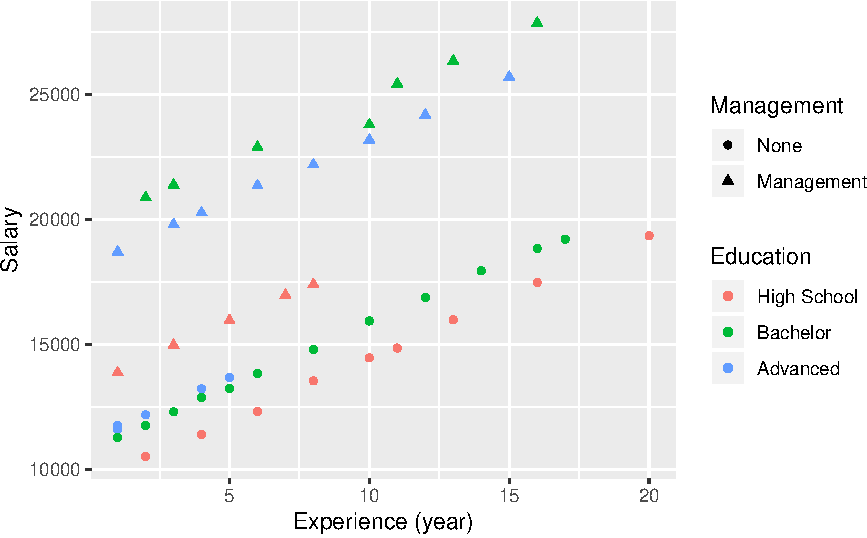
\includegraphics[width=0.7\linewidth]{regression-analysis_files/figure-latex/sald-1} 

}

\caption{Salary Survey Data}\label{fig:sald}
\end{figure}

See Figure \ref{fig:sald}. There are 6 combinations of \texttt{E}-\texttt{M}. For each level, we can see obvious linear relationship between \texttt{S} (salary) and \texttt{X} (experience). Also, person in management statement has larer salary than not. How can we deal with these variables?

\hypertarget{modsep}{%
\subsection{Separate models}\label{modsep}}

The easiest way that we can think of is fit separate regression models for

\begin{enumerate}
\def\labelenumi{\arabic{enumi}.}
\tightlist
\item
  different levels of the qualitative predictor (in case there is only one qualitative predictor)
\item
  \emph{different combinations of the levels.}
\end{enumerate}

In the above salary survey dataset, we can make 6 models.

\begin{longtable}[]{@{}cccc@{}}
\toprule
\begin{minipage}[b]{0.25\columnwidth}\centering
levels\strut
\end{minipage} & \begin{minipage}[b]{0.21\columnwidth}\centering
HS\strut
\end{minipage} & \begin{minipage}[b]{0.21\columnwidth}\centering
BS\strut
\end{minipage} & \begin{minipage}[b]{0.21\columnwidth}\centering
ADV\strut
\end{minipage}\tabularnewline
\midrule
\endhead
\begin{minipage}[t]{0.25\columnwidth}\centering
MGT\strut
\end{minipage} & \begin{minipage}[t]{0.21\columnwidth}\centering
\(Y_i = \beta_{01} + \beta_{11} x_i + \epsilon_{i1}\)\strut
\end{minipage} & \begin{minipage}[t]{0.21\columnwidth}\centering
\(Y_i = \beta_{02} + \beta_{12} x_i + \epsilon_{i2}\)\strut
\end{minipage} & \begin{minipage}[t]{0.21\columnwidth}\centering
\(Y_i = \beta_{03} + \beta_{13} x_i + \epsilon_{i3}\)\strut
\end{minipage}\tabularnewline
\begin{minipage}[t]{0.25\columnwidth}\centering
None\strut
\end{minipage} & \begin{minipage}[t]{0.21\columnwidth}\centering
\(Y_i = \beta_{04} + \beta_{14} x_i + \epsilon_{i4}\)\strut
\end{minipage} & \begin{minipage}[t]{0.21\columnwidth}\centering
\(Y_i = \beta_{05} + \beta_{15} x_i + \epsilon_{i5}\)\strut
\end{minipage} & \begin{minipage}[t]{0.21\columnwidth}\centering
\(Y_i = \beta_{06} + \beta_{16} x_i + \epsilon_{i6}\)\strut
\end{minipage}\tabularnewline
\bottomrule
\end{longtable}

\hypertarget{moddummy1}{%
\subsection{Dummy variables}\label{moddummy1}}

However, we want to explain linear relationship between response variable and qualitative predictors. Commonly, this is done by defining \textbf{dummy variables} or \textbf{indicator variables}. For instance, Define \(E_{i1}\) and \(E_{i2}\) by

\begin{equation*}
  \begin{split}
    & E_{i1} = \begin{cases}
      1 & E = HS \\
      0 & \text{o/w}
    \end{cases} \\
    & E_{i2} = \begin{cases}
      1 & E = BS \\
      0 & \text{o/w}
    \end{cases}
  \end{split}
\end{equation*}

In other words, the last level ADV(\texttt{3}) has value of \(E_{i1} = E_{i2} = 0\). This is called \emph{dummy coding} of the last level as baseline. The following function gives how the coding is happened. In \texttt{R}, baseline is set to be the first level, i.e.~\texttt{base\ =\ 1} by default.

\begin{Shaded}
\begin{Highlighting}[]
\KeywordTok{C}\NormalTok{(salary}\OperatorTok{$}\NormalTok{E, }\DataTypeTok{contr =}\NormalTok{ contr.treatment, }\DataTypeTok{base =} \DecValTok{3}\NormalTok{)}
\CommentTok{#>  [1] 1 3 3 2 3 2 2 1 3 2 1 2 3 1 3 3 2 2 3 1 1 3 2 2 1 2 1 3 1 1 2 3 2 2 1}
\CommentTok{#> [36] 2 3 1 2 2 3 2 2 1 2 1}
\CommentTok{#> attr(,"contrasts")}
\CommentTok{#>   1 2}
\CommentTok{#> 1 1 0}
\CommentTok{#> 2 0 1}
\CommentTok{#> 3 0 0}
\CommentTok{#> Levels: 1 2 3}
\end{Highlighting}
\end{Shaded}

For management status, define \(MGT_i\) by

\[
MGT_i = \begin{cases}
  1 & M = MGT \\
  0 & M = None
\end{cases}
\]

This is the case when \texttt{base\ =\ 1}, i.e.~\texttt{0}(None) in our data set.

\begin{Shaded}
\begin{Highlighting}[]
\KeywordTok{C}\NormalTok{(salary}\OperatorTok{$}\NormalTok{M, }\DataTypeTok{contr =}\NormalTok{ contr.treatment)}
\CommentTok{#>  [1] 1 0 1 0 0 1 0 0 0 0 1 1 1 0 1 0 0 0 0 1 0 1 0 1 1 0 1 1 0 0 0 1 1 1 0}
\CommentTok{#> [36] 0 1 0 1 0 1 1 0 0 0 0}
\CommentTok{#> attr(,"contrasts")}
\CommentTok{#>   2}
\CommentTok{#> 0 0}
\CommentTok{#> 1 1}
\CommentTok{#> Levels: 0 1}
\end{Highlighting}
\end{Shaded}

The we now have regression model as

\begin{equation}
  Y_i = \beta_0 + \beta_1 x_i + \gamma_1 E_{i1} + \gamma_2 E_{i2} + \delta MGT_i + \epsilon_i
  \label{eq:dummymod}
\end{equation}

\begin{Shaded}
\begin{Highlighting}[]
\NormalTok{salary_relev <-}
\StringTok{  }\NormalTok{salary }\OperatorTok\StringTok{ }
\StringTok{  }\KeywordTok{mutate}\NormalTok{(}
    \DataTypeTok{E =} \KeywordTok{C}\NormalTok{(E, }\DataTypeTok{contr =}\NormalTok{ contr.treatment, }\DataTypeTok{base =} \DecValTok{3}\NormalTok{) }\CommentTok{# different with default}
\NormalTok{  )}
\CommentTok{#--------------}
\NormalTok{salary_relev }\OperatorTok\StringTok{ }
\StringTok{  }\KeywordTok{lm}\NormalTok{(S }\OperatorTok{~}\StringTok{ }\NormalTok{., }\DataTypeTok{data =}\NormalTok{ .)}
\CommentTok{#> }
\CommentTok{#> Call:}
\CommentTok{#> lm(formula = S ~ ., data = .)}
\CommentTok{#> }
\CommentTok{#> Coefficients:}
\CommentTok{#> (Intercept)            X           E1           E2           M1  }
\CommentTok{#>       11032          546        -2996          148         6884}
\end{Highlighting}
\end{Shaded}

Plug in each value. Then we can make 6 models as previous section.

\begin{equation}
  \begin{cases}
    Y_i = (\beta_0 + \gamma_1) + \beta_1 x_i + \epsilon_i & \text{HS-None} \qquad E_1 = 1, E_2 = 0, MGT = 0 \\
    Y_i = (\beta_0 + \gamma_1 + \delta) + \beta_1 x_i + \epsilon_i & \text{HS-MGT} \qquad E_1 = 1, E_2 = 0, MGT = 1 \\
    Y_i = (\beta_0 + \gamma_2) + \beta_1 x_i + \epsilon_i & \text{BS-None} \qquad E_1 = 0, E_2 = 1, MGT = 0 \\
    Y_i = (\beta_0 + \gamma_2 + \delta) + \beta_1 x_i + \epsilon_i & \text{BS-MGT} \qquad E_1 = 0, E_2 = 1, MGT = 1 \\
    Y_i = \beta_0 + \beta_1 x_i + \epsilon_i & \text{ADV-None} \qquad E_1 = 0, E_2 = 0, MGT = 0 \\
    Y_i = (\beta_0 + \delta) + \beta_1 x_i + \epsilon_i & \text{ADV-MGT} \qquad E_1 = 0, E_2 = 0, MGT = 1
  \end{cases}
  \label{eq:dummysep}
\end{equation}

Observe that every line has same slope \(\beta_1\).

\begin{Shaded}
\begin{Highlighting}[]
\NormalTok{salary_relev }\OperatorTok\StringTok{ }
\StringTok{  }\KeywordTok{ggplot}\NormalTok{(}\KeywordTok{aes}\NormalTok{(}\DataTypeTok{x =}\NormalTok{ X, }\DataTypeTok{y =}\NormalTok{ S, }\DataTypeTok{colour =}\NormalTok{ E, }\DataTypeTok{linetype =}\NormalTok{ M)) }\OperatorTok{+}
\StringTok{  }\KeywordTok{geom_smooth}\NormalTok{(}\DataTypeTok{method =} \StringTok{"lm"}\NormalTok{, }\DataTypeTok{se =} \OtherTok{FALSE}\NormalTok{, }\DataTypeTok{fullrange =} \OtherTok{TRUE}\NormalTok{) }\OperatorTok{+}
\StringTok{  }\KeywordTok{geom_point}\NormalTok{(}\KeywordTok{aes}\NormalTok{(}\DataTypeTok{shape =}\NormalTok{ M), }\DataTypeTok{alpha =} \FloatTok{.7}\NormalTok{, }\DataTypeTok{show.legend =} \OtherTok{FALSE}\NormalTok{) }\OperatorTok{+}
\StringTok{  }\KeywordTok{labs}\NormalTok{(}
    \DataTypeTok{x =} \StringTok{"Experience (year)"}\NormalTok{,}
    \DataTypeTok{y =} \StringTok{"Salary"}
\NormalTok{  ) }\OperatorTok{+}
\StringTok{  }\KeywordTok{scale_colour_discrete}\NormalTok{(}
    \DataTypeTok{name =} \StringTok{"Education"}\NormalTok{,}
    \DataTypeTok{label =} \KeywordTok{c}\NormalTok{(}\StringTok{"High School"}\NormalTok{, }\StringTok{"Bachelor"}\NormalTok{, }\StringTok{"Advanced"}\NormalTok{)}
\NormalTok{  ) }\OperatorTok{+}
\StringTok{  }\KeywordTok{scale_linetype_discrete}\NormalTok{(}
    \DataTypeTok{name =} \StringTok{"Management"}\NormalTok{,}
    \DataTypeTok{label =} \KeywordTok{c}\NormalTok{(}\StringTok{"None"}\NormalTok{, }\StringTok{"Management"}\NormalTok{)}
\NormalTok{  )}
\end{Highlighting}
\end{Shaded}

\begin{figure}[H]

{\centering 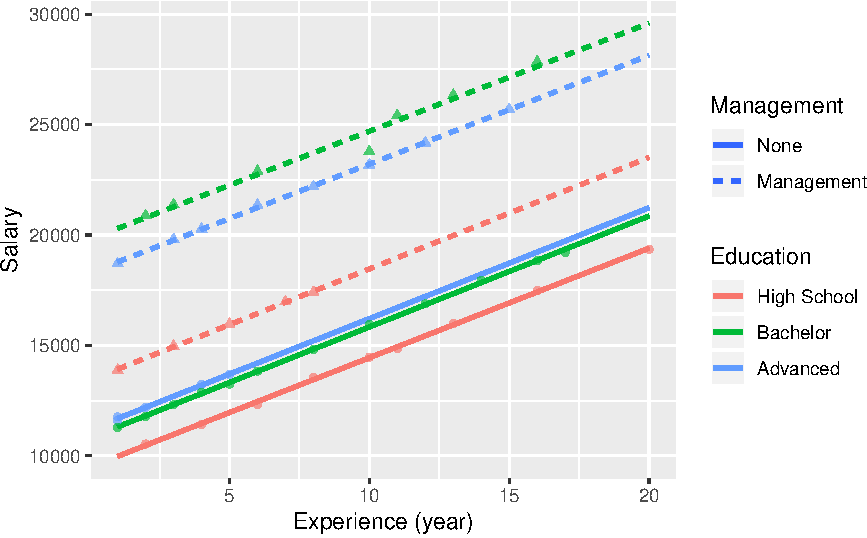
\includegraphics[width=0.7\linewidth]{regression-analysis_files/figure-latex/saldfit-1} 

}

\caption{Salary Survey Data with Dummy variables}\label{fig:saldfit}
\end{figure}

Every line is parallel to each other. In the set of Equations \eqref{eq:dummysep}, we can interpret \(\beta_1\) as the increment of salary when experience increases in 1 year \emph{when the other predictors are fixed}.

\(\gamma_1\), the coefficient of \(E_{i1}\), can be interpreted as the increment of salary for \texttt{HS} compared to \texttt{ADV}(baseline) when the other predictors are fixed. Similarly, we interpret \(\gamma_2\), the coefficient of \(E_{i2}\) as the increment of salary for \texttt{BS} compared to the baseline level \texttt{ADV} when the other predictors are fixed. The coefficient of \(MGT\) \(\delta\) means the increment of salary for management status for none when the other predictors fixed.

In sum, each coefficient for dummy variables is the increment for corresponding level versus baseline level.

\hypertarget{moddummy2}{%
\subsection{Interaction variables}\label{moddummy2}}

See Figure \ref{fig:sald} and focus on education level. Among people in management responsibility, ones with bachelor degrees have the largest salaries and next advanced dgrees. On the other hand, advanced degrees seem to be more important than bachelor among people that are not in management status. The \emph{magnitude of the salary difference between education level also depends management status}. To explain this, we add \emph{interaction term} in the previous model \eqref{eq:dummymod}.

\begin{equation}
  Y_i = \beta_0 + \beta_1 x_i + \gamma_1 E_{i1} + \gamma_2 E_{i2} + \delta MGT_i + {\color{blue}{\alpha_1 (E_{i1} MGT_i)}} + {\color{blue}{\alpha_2 (E_{i2} MGT_i)}} + \epsilon_i
  \label{eq:dummymod2}
\end{equation}

\begin{Shaded}
\begin{Highlighting}[]
\NormalTok{(dum_int1 <-}
\StringTok{  }\NormalTok{salary_relev }\OperatorTok\StringTok{ }
\StringTok{  }\KeywordTok{lm}\NormalTok{(S }\OperatorTok{~}\StringTok{ }\NormalTok{X }\OperatorTok{+}\StringTok{ }\NormalTok{E }\OperatorTok{*}\StringTok{ }\NormalTok{M, }\DataTypeTok{data =}\NormalTok{ .))}
\CommentTok{#> }
\CommentTok{#> Call:}
\CommentTok{#> lm(formula = S ~ X + E * M, data = .)}
\CommentTok{#> }
\CommentTok{#> Coefficients:}
\CommentTok{#> (Intercept)            X           E1           E2           M1  }
\CommentTok{#>       11203          497        -1731         -349         7047  }
\CommentTok{#>       E1:M1        E2:M1  }
\CommentTok{#>       -3066         1836}
\end{Highlighting}
\end{Shaded}

\begin{equation}
  \begin{cases}
    Y_i = (\beta_0 + \gamma_1) + \beta_1 x_i + \epsilon_i & \text{HS-None} \qquad E_1 = 1, E_2 = 0, MGT = 0 \\
    Y_i = (\beta_0 + \gamma_1 + \delta + {\color{blue}{\alpha_1}}) + \beta_1 x_i + \epsilon_i & \text{HS-MGT} \qquad E_1 = 1, E_2 = 0, MGT = 1 \\
    Y_i = (\beta_0 + \gamma_2) + \beta_1 x_i + \epsilon_i & \text{BS-None} \qquad E_1 = 0, E_2 = 1, MGT = 0 \\
    Y_i = (\beta_0 + \gamma_2 + \delta + {\color{blue}{\alpha_2}}) + \beta_1 x_i + \epsilon_i & \text{BS-MGT} \qquad E_1 = 0, E_2 = 1, MGT = 1 \\
    Y_i = \beta_0 + \beta_1 x_i + \epsilon_i & \text{ADV-None} \qquad E_1 = 0, E_2 = 0, MGT = 0 \\
    Y_i = (\beta_0 + \delta) + \beta_1 x_i + \epsilon_i & \text{ADV-MGT} \qquad E_1 = 0, E_2 = 0, MGT = 1
  \end{cases}
  \label{eq:dummysep2}
\end{equation}

To visualize the model, i.e.~get prediction for each grid, we might use \texttt{modelr} library.

\begin{Shaded}
\begin{Highlighting}[]
\KeywordTok{library}\NormalTok{(modelr)}
\end{Highlighting}
\end{Shaded}

\texttt{modelr::data\_grid()} expands predictor grids for prediction. \texttt{modelr::add\_predictions()} add predictions for a given model to a data frame. We can provide multiple models with \texttt{modelr::spread\_predictions()} and \texttt{modelr::gather\_predictions()} each as \texttt{tidyr::spread()} and \texttt{tidyr::gather()}.

\begin{Shaded}
\begin{Highlighting}[]
\NormalTok{salary_relev }\OperatorTok\StringTok{ }
\StringTok{  }\KeywordTok{data_grid}\NormalTok{(X, E, M) }\OperatorTok\StringTok{ }
\StringTok{  }\KeywordTok{add_predictions}\NormalTok{(dum_int1) }\OperatorTok\StringTok{ }
\StringTok{  }\KeywordTok{ggplot}\NormalTok{() }\OperatorTok{+}
\StringTok{  }\KeywordTok{geom_line}\NormalTok{(}\KeywordTok{aes}\NormalTok{(}\DataTypeTok{x =}\NormalTok{ X, }\DataTypeTok{y =}\NormalTok{ pred, }\DataTypeTok{colour =}\NormalTok{ E, }\DataTypeTok{linetype =}\NormalTok{ M)) }\OperatorTok{+}
\StringTok{  }\KeywordTok{geom_point}\NormalTok{(}
    \DataTypeTok{data =}\NormalTok{ salary_relev, }
    \KeywordTok{aes}\NormalTok{(}\DataTypeTok{x =}\NormalTok{ X, }\DataTypeTok{y =}\NormalTok{ S, }\DataTypeTok{colour =}\NormalTok{ E, }\DataTypeTok{shape =}\NormalTok{ M), }
    \DataTypeTok{alpha =} \FloatTok{.7}\NormalTok{, }
    \DataTypeTok{show.legend =} \OtherTok{FALSE}
\NormalTok{  ) }\OperatorTok{+}
\StringTok{  }\KeywordTok{labs}\NormalTok{(}
    \DataTypeTok{x =} \StringTok{"Experience (year)"}\NormalTok{,}
    \DataTypeTok{y =} \StringTok{"Salary"}
\NormalTok{  ) }\OperatorTok{+}
\StringTok{  }\KeywordTok{scale_colour_discrete}\NormalTok{(}
    \DataTypeTok{name =} \StringTok{"Education"}\NormalTok{,}
    \DataTypeTok{label =} \KeywordTok{c}\NormalTok{(}\StringTok{"High School"}\NormalTok{, }\StringTok{"Bachelor"}\NormalTok{, }\StringTok{"Advanced"}\NormalTok{)}
\NormalTok{  ) }\OperatorTok{+}
\StringTok{  }\KeywordTok{scale_linetype_discrete}\NormalTok{(}
    \DataTypeTok{name =} \StringTok{"Management"}\NormalTok{,}
    \DataTypeTok{label =} \KeywordTok{c}\NormalTok{(}\StringTok{"None"}\NormalTok{, }\StringTok{"Management"}\NormalTok{)}
\NormalTok{  )}
\end{Highlighting}
\end{Shaded}

\begin{figure}[H]

{\centering 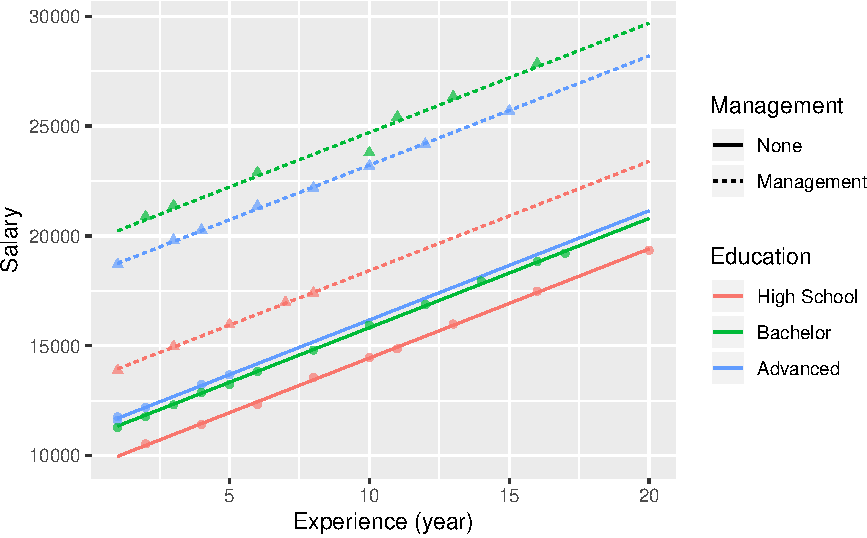
\includegraphics[width=0.7\linewidth]{regression-analysis_files/figure-latex/saldfit2-1} 

}

\caption{Interaction between qualitative variables}\label{fig:saldfit2}
\end{figure}

Here the increment for experience is also same for each level.

\hypertarget{general-models-with-interaction}{%
\subsection{General models with interaction}\label{general-models-with-interaction}}

In the previous section \ref{moddummy1} and \ref{moddummy2}, there have been some assumptions in the model. In Model \eqref{eq:dummymod}, \emph{additive assumption} is given. Effects of each predictors do note depend on the others. It means that in the separate model setting \ref{modsep} we give conditions

\[
\begin{cases}
  \beta_{11} = \beta_{12} = \cdots = \beta_{16} \equiv \beta_1 \\
  \beta_{01} - \beta_{04} = \beta_{02} - \beta_{05} = \beta_{03} - \beta_{06} \equiv \delta
\end{cases}
\]

Next model \eqref{eq:dummymod2} quite weakens this assumption, i.e.~remove the second condition for \(\delta\) by adding an interaction term between qualitative predictors. Instead, it still assumes that \emph{every combination of levels always has same slope} \(\beta_1\). Now we want more general one without the first assumption. Add interaction between \(x_i\) and other dummy variables.

\begin{equation}
  \begin{split}
    Y_i = \beta_0 & + \beta_1 x_i + \gamma_1 E_{i1} + \gamma_2 E_{i2} + \delta MGT_i \\
    & + {\color{blue}{\alpha_1 (E_{i1} MGT_i)}} + {\color{blue}{\alpha_2 (E_{i2} MGT_i)}} \\
    & + {\color{red}{\eta_1(x_i E_{i1})}} + {\color{red}{\eta_2(x_i E_{i2})}} + {\color{red}{\eta_3(x_i MGT_i)}} \\
    & + {\color{red}{\eta_4(x_i MGT_i E_{i1})}} + {\color{red}{\eta_5(x_i MGT_i E_{i2})}} \\
    & + \epsilon_i
  \end{split}
  \label{eq:dummymod3}
\end{equation}

\begin{Shaded}
\begin{Highlighting}[]
\NormalTok{(dum_int2 <-}
\StringTok{  }\NormalTok{salary_relev }\OperatorTok\StringTok{ }
\StringTok{  }\KeywordTok{lm}\NormalTok{(S }\OperatorTok{~}\StringTok{ }\NormalTok{X }\OperatorTok{*}\StringTok{ }\NormalTok{E }\OperatorTok{*}\StringTok{ }\NormalTok{M, }\DataTypeTok{data =}\NormalTok{ .))}
\CommentTok{#> }
\CommentTok{#> Call:}
\CommentTok{#> lm(formula = S ~ X * E * M, data = .)}
\CommentTok{#> }
\CommentTok{#> Coefficients:}
\CommentTok{#> (Intercept)            X           E1           E2           M1  }
\CommentTok{#>   11189.455      502.364    -1708.064     -381.019     7094.382  }
\CommentTok{#>        X:E1         X:E2         X:M1        E1:M1        E2:M1  }
\CommentTok{#>      -6.247        0.246       -9.850    -3158.650     1904.041  }
\CommentTok{#>     X:E1:M1      X:E2:M1  }
\CommentTok{#>      18.416       -3.645}
\end{Highlighting}
\end{Shaded}

In the same process, we have separate model. Since we have added terms with \(x_i\), the only change from Equation \eqref{eq:dummysep2} is slope part.

\begin{equation}
  \begin{alignedat}{5}
    & Y_i = (\beta_0 + \gamma_1) && + (\beta_1 + {\color{red}{\eta_1}}) x_i && + \epsilon_i && \quad \text{HS-None} && \quad E_1 = 1, E_2 = 0, MGT = 0 \\
    & Y_i = (\beta_0 + \gamma_1 + \delta + {\color{blue}{\alpha_1}}) && + (\beta_1 + {\color{red}{\eta_1}} + {\color{red}{\eta_3}} + {\color{red}{\eta_4}}) x_i && + \epsilon_i && \quad \text{HS-MGT} && \quad E_1 = 1, E_2 = 0, MGT = 1 \\
    & Y_i = (\beta_0 + \gamma_2) && + (\beta_1 + {\color{red}{\eta_2}}) x_i && + \epsilon_i && \quad \text{BS-None} && \quad E_1 = 0, E_2 = 1, MGT = 0 \\
    & Y_i = (\beta_0 + \gamma_2 + \delta + {\color{blue}{\alpha_2}}) && + (\beta_1 + {\color{red}{\eta_2}} + {\color{red}{\eta_3}} + {\color{red}{\eta_5}}) x_i && + \epsilon_i && \quad \text{BS-MGT} && \quad E_1 = 0, E_2 = 1, MGT = 1 \\
    & Y_i = \beta_0 && + \beta_1 x_i && + \epsilon_i && \quad \text{ADV-None} && \quad E_1 = 0, E_2 = 0, MGT = 0 \\
    & Y_i = (\beta_0 + \delta) && + (\beta_1 + {\color{red}{\eta_3}}) x_i && + \epsilon_i && \quad \text{ADV-MGT} && \quad E_1 = 0, E_2 = 0, MGT = 1
  \end{alignedat}
  \label{eq:dummysep3}
\end{equation}

\begin{Shaded}
\begin{Highlighting}[]
\NormalTok{salary_relev }\OperatorTok\StringTok{ }
\StringTok{  }\KeywordTok{data_grid}\NormalTok{(X, E, M) }\OperatorTok\StringTok{ }
\StringTok{  }\KeywordTok{add_predictions}\NormalTok{(dum_int2) }\OperatorTok\StringTok{ }
\StringTok{  }\KeywordTok{ggplot}\NormalTok{() }\OperatorTok{+}
\StringTok{  }\KeywordTok{geom_line}\NormalTok{(}\KeywordTok{aes}\NormalTok{(}\DataTypeTok{x =}\NormalTok{ X, }\DataTypeTok{y =}\NormalTok{ pred, }\DataTypeTok{colour =}\NormalTok{ E, }\DataTypeTok{linetype =}\NormalTok{ M)) }\OperatorTok{+}
\StringTok{  }\KeywordTok{geom_point}\NormalTok{(}
    \DataTypeTok{data =}\NormalTok{ salary_relev, }
    \KeywordTok{aes}\NormalTok{(}\DataTypeTok{x =}\NormalTok{ X, }\DataTypeTok{y =}\NormalTok{ S, }\DataTypeTok{colour =}\NormalTok{ E, }\DataTypeTok{shape =}\NormalTok{ M), }
    \DataTypeTok{alpha =} \FloatTok{.7}\NormalTok{, }
    \DataTypeTok{show.legend =} \OtherTok{FALSE}
\NormalTok{  ) }\OperatorTok{+}
\StringTok{  }\KeywordTok{labs}\NormalTok{(}
    \DataTypeTok{x =} \StringTok{"Experience (year)"}\NormalTok{,}
    \DataTypeTok{y =} \StringTok{"Salary"}
\NormalTok{  ) }\OperatorTok{+}
\StringTok{  }\KeywordTok{scale_colour_discrete}\NormalTok{(}
    \DataTypeTok{name =} \StringTok{"Education"}\NormalTok{,}
    \DataTypeTok{label =} \KeywordTok{c}\NormalTok{(}\StringTok{"High School"}\NormalTok{, }\StringTok{"Bachelor"}\NormalTok{, }\StringTok{"Advanced"}\NormalTok{)}
\NormalTok{  ) }\OperatorTok{+}
\StringTok{  }\KeywordTok{scale_linetype_discrete}\NormalTok{(}
    \DataTypeTok{name =} \StringTok{"Management"}\NormalTok{,}
    \DataTypeTok{label =} \KeywordTok{c}\NormalTok{(}\StringTok{"None"}\NormalTok{, }\StringTok{"Management"}\NormalTok{)}
\NormalTok{  )}
\end{Highlighting}
\end{Shaded}

\begin{figure}[H]

{\centering 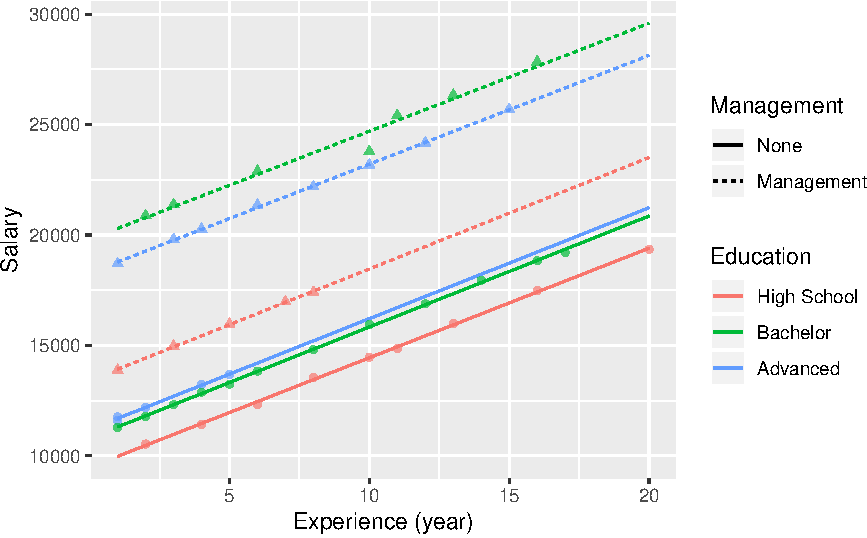
\includegraphics[width=0.7\linewidth]{regression-analysis_files/figure-latex/saldfit3-1} 

}

\caption{Full interaction model}\label{fig:saldfit3}
\end{figure}

\begin{Shaded}
\begin{Highlighting}[]
\KeywordTok{summary}\NormalTok{(dum_int2)}
\CommentTok{#> }
\CommentTok{#> Call:}
\CommentTok{#> lm(formula = S ~ X * E * M, data = .)}
\CommentTok{#> }
\CommentTok{#> Residuals:}
\CommentTok{#>    Min     1Q Median     3Q    Max }
\CommentTok{#> -918.0  -41.2   14.2   64.8  222.9 }
\CommentTok{#> }
\CommentTok{#> Coefficients:}
\CommentTok{#>              Estimate Std. Error t value Pr(>|t|)    }
\CommentTok{#> (Intercept) 11189.455    155.304   72.05  < 2e-16 ***}
\CommentTok{#> X             502.364     50.655    9.92  1.4e-11 ***}
\CommentTok{#> E1          -1708.064    201.534   -8.48  6.7e-10 ***}
\CommentTok{#> E2           -381.019    183.282   -2.08    0.045 *  }
\CommentTok{#> M1           7094.382    199.690   35.53  < 2e-16 ***}
\CommentTok{#> X:E1           -6.247     51.896   -0.12    0.905    }
\CommentTok{#> X:E2            0.246     51.630    0.00    0.996    }
\CommentTok{#> X:M1           -9.850     52.704   -0.19    0.853    }
\CommentTok{#> E1:M1       -3158.650    294.852  -10.71  1.9e-12 ***}
\CommentTok{#> E2:M1        1904.041    264.434    7.20  2.5e-08 ***}
\CommentTok{#> X:E1:M1        18.416     62.751    0.29    0.771    }
\CommentTok{#> X:E2:M1        -3.645     55.540   -0.07    0.948    }
\CommentTok{#> ---}
\CommentTok{#> Signif. codes:  0 '***' 0.001 '**' 0.01 '*' 0.05 '.' 0.1 ' ' 1}
\CommentTok{#> }
\CommentTok{#> Residual standard error: 184 on 34 degrees of freedom}
\CommentTok{#> Multiple R-squared:  0.999,  Adjusted R-squared:  0.998 }
\CommentTok{#> F-statistic: 2.68e+03 on 11 and 34 DF,  p-value: <2e-16}
\end{Highlighting}
\end{Shaded}

Denote that the changes of slopes are not that significant.

\hypertarget{regression-approach-to-anova}{%
\subsection{Regression approach to ANOVA}\label{regression-approach-to-anova}}

We have generated three grouped data of which group is three.

\begin{Shaded}
\begin{Highlighting}[]
\NormalTok{medicine}
\CommentTok{#> # A tibble: 90 x 2}
\CommentTok{#>   trt       y}
\CommentTok{#>   <fct> <dbl>}
\CommentTok{#> 1 1     1.87 }
\CommentTok{#> 2 1     0.400}
\CommentTok{#> 3 1     0.283}
\CommentTok{#> 4 1     1.70 }
\CommentTok{#> 5 1     2.23 }
\CommentTok{#> 6 1     1.27 }
\CommentTok{#> # ... with 84 more rows}
\end{Highlighting}
\end{Shaded}

\begin{Shaded}
\begin{Highlighting}[]
\NormalTok{medicine }\OperatorTok\StringTok{ }
\StringTok{  }\KeywordTok{group_by}\NormalTok{(trt) }\OperatorTok\StringTok{ }
\StringTok{  }\KeywordTok{summarise}\NormalTok{(}\DataTypeTok{m =} \KeywordTok{mean}\NormalTok{(y), }\DataTypeTok{s =} \KeywordTok{sd}\NormalTok{(y), }\DataTypeTok{N =} \KeywordTok{n}\NormalTok{())}
\CommentTok{#> # A tibble: 3 x 4}
\CommentTok{#>   trt       m     s     N}
\CommentTok{#>   <fct> <dbl> <dbl> <int>}
\CommentTok{#> 1 1     0.881 0.818    30}
\CommentTok{#> 2 2     2.17  1.15     30}
\CommentTok{#> 3 3     3.02  0.940    30}
\end{Highlighting}
\end{Shaded}

\begin{Shaded}
\begin{Highlighting}[]
\NormalTok{medicine }\OperatorTok\StringTok{ }
\StringTok{  }\KeywordTok{ggplot}\NormalTok{(}\KeywordTok{aes}\NormalTok{(}\DataTypeTok{x =}\NormalTok{ trt, }\DataTypeTok{y =}\NormalTok{ y, }\DataTypeTok{fill =}\NormalTok{ trt)) }\OperatorTok{+}
\StringTok{  }\KeywordTok{geom_boxplot}\NormalTok{(}\DataTypeTok{show.legend =} \OtherTok{FALSE}\NormalTok{)}
\end{Highlighting}
\end{Shaded}

\begin{center}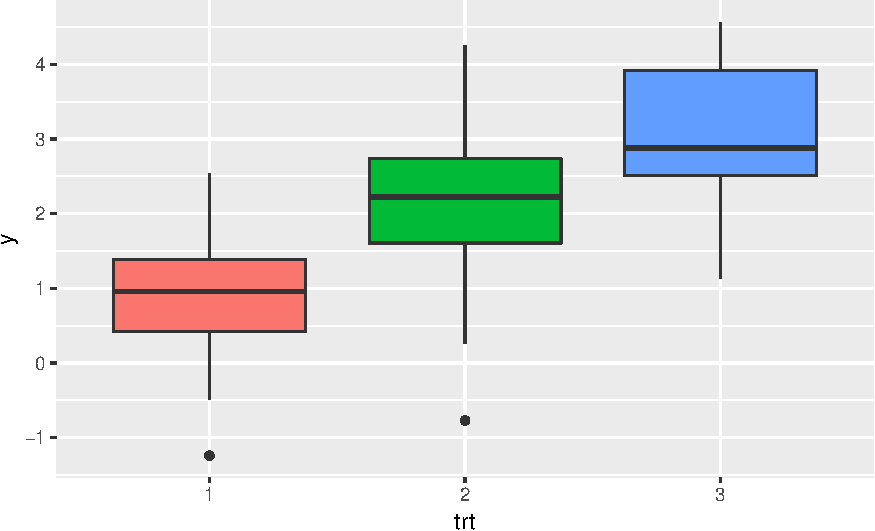
\includegraphics[width=0.7\linewidth]{regression-analysis_files/figure-latex/unnamed-chunk-110-1} \end{center}

Each group follows \(N(\mu_1 = 1, \sigma^2 = 1)\), \(N(\mu_2 = 2, \sigma^2 = 1)\), and \(N(\mu_3 = 3, \sigma^2 = 1)\). Our goal is comparison between treatment, i.e.~mean comparison.

\[H_0: \mu_1 = \mu_2 = \mu_3 \quad \text{vs} \quad H_1: \text{not}\: H_0\]

\begin{Shaded}
\begin{Highlighting}[]
\KeywordTok{aov}\NormalTok{(y }\OperatorTok{~}\StringTok{ }\NormalTok{trt, }\DataTypeTok{data =}\NormalTok{ medicine) }\OperatorTok\StringTok{ }
\StringTok{  }\KeywordTok{summary}\NormalTok{()}
\CommentTok{#>             Df Sum Sq Mean Sq F value  Pr(>F)    }
\CommentTok{#> trt          2   69.5    34.7    36.3 3.5e-12 ***}
\CommentTok{#> Residuals   87   83.3     1.0                    }
\CommentTok{#> ---}
\CommentTok{#> Signif. codes:  0 '***' 0.001 '**' 0.01 '*' 0.05 '.' 0.1 ' ' 1}
\end{Highlighting}
\end{Shaded}

Recall that we can build two models, \emph{means model} or \emph{effects model}.

\hypertarget{effects-model}{%
\subsection{Effects model}\label{effects-model}}

In experimental design literature, effects model is more frequently used. Decomposing each group mean with overall mean and \emph{treatment effect}, it gives more intuitive decription \citep{Montgomery:2012aa}. So we look at this one first.

\begin{equation}
  Y_{ij} = \mu + \tau_j + \epsilon_{ij}
  \label{eq:effmod}
\end{equation}

where

\[
\begin{cases}
  1 \le i \le n_j \\
  1 \le j \le k & j \text{: treatment} \\
  Y_{ij} = i \text{-th observation from the}\: j \text{-th treatment} \\
  \mu = \text{overall mean} \\
  \tau_j = j \text{-th treatment effect} := \mu_j - \mu \\
  \epsilon_{ij} \stackrel{iid}{\sim}N(0, \sigma^2)
\end{cases}
\]

Here we test whether there is \emph{no treatment effect}, i.e.

\[H_0: \tau_1 = \cdots = \tau_k = 0 \quad \text{vs} \quad H_1: \text{not}\: H_0\]

which is equivalent to the above \(\mu_1 = \cdots = \mu_k\) by construction.

Note that we have \(k + 1\) parameters in the model \eqref{eq:effmod}. Write the parameter vector as

\[\boldsymbol\theta \equiv (\mu, \tau_1, \ldots, \tau_k)^T\]

Then we can express the model as

\[
\underset{\huge \mathbf{Y}}{\begin{bmatrix}
  Y_{11} \\
  Y_{21} \\
  \vdots \\
  Y_{n_1, 1} \\ \hline
  Y_{12} \\
  \vdots \\
  Y_{n_2, 2} \\ \hline
  \vdots \\ \hline
  Y_{1k} \\
  \vdots \\
  Y_{n_k, k}
\end{bmatrix}} = \underset{\huge X}{\begin{bmatrix}
  1 & 1 & 0 & \cdots & 0 \\
  1 & 1 & 0 & \cdots & 0 \\
  \vdots & \vdots & \vdots & \vdots & \vdots \\
  1 & 1 & 0 & \cdots & 0 \\ \hline
  1 & 0 & 1 & \cdots & 0 \\
  \vdots & \vdots & \vdots & \vdots & \vdots \\
  1 & 0 & 1 & \cdots & 0 \\ \hline
  \vdots & \vdots & \vdots & \vdots & \vdots \\ \hline
  1 & 0 & 0 & \cdots & 1 \\
  \vdots & \vdots & \vdots & \vdots & \vdots \\
  1 & 0 & 0 & \cdots & 1
\end{bmatrix}} \underset{\huge \boldsymbol\theta}{\begin{bmatrix}
  \mu \\
  \tau_1 \\
  \vdots \\
  \tau_k
\end{bmatrix}} + \underset{\huge \E}{\begin{bmatrix}
  \epsilon_{11} \\
  \epsilon_{21} \\
  \vdots \\
  \epsilon_{n_1, 1} \\ \hline
  \epsilon_{12} \\
  \vdots \\
  \epsilon_{n_2, 2} \\ \hline
  \vdots \\ \hline
  \epsilon_{1k} \\
  \vdots \\
  \epsilon_{n_k,k}
\end{bmatrix}}
\]

Look at the model matrix \(X = \begin{bmatrix} \mathbf{1} \mid \mathbf{x}_1 \mid \cdots \mid \mathbf{x}_k \end{bmatrix} \in \mathbb{R}^{N \times (k + 1)}\), where \(N = \sum n_j\). From the second column to the last, \(\mathbf{x}_j = (x_{1j}, \ldots, x_{n_j, j})\) has value of

\[
x_{ij} = \begin{cases}
  1 & j\text{-th treatment} \\
  0 & \text{otherwise}
\end{cases}
\]

However,

\[\mathbf{1} = \mathbf{x}_1 + \cdots + \mathbf{x}_k\]

i.e.~linearly independent. This design matrix \(X\) is of rank deficient. Hence, the normal equation \((X^TX)^{-1}\boldsymbol{\hat\beta}= X^T \mathbf{Y}\) does \emph{not have a unique solution}. This kind of coding is not appropriate. \citet{Rawlings:2006aa} provides four ways \emph{reparameterizing} to remove singularities.

\hypertarget{means-model}{%
\subsection{Means model}\label{means-model}}

Next, consider means model.

\begin{equation}
  Y_{ij} = \mu_j + \epsilon_{ij}
  \label{eq:meanmod}
\end{equation}

where

\[
\begin{cases}
  1 \le i \le n_j \\
  1 \le j \le k & j \text{: treatment} \\
  Y_{ij} = i \text{-th observation from the}\: j \text{-th treatment} \\
  \mu_j = \text{mean of}\: j \text{-th treatment} \\
  \epsilon_{ij} \stackrel{iid}{\sim}N(0, \sigma^2)
\end{cases}
\]

With this model \eqref{eq:meanmod}, we test if every \(\mu_j\) is identical.

\[H_0: \mu_1 = \cdots = \mu_k \quad \text{vs} \quad H_1: \text{not}\: H_0\]

Write a parameter vector by

\[\boldsymbol\theta^{\ast} \equiv (\mu_1, \ldots, \mu_k)^T \in \mathbb{R}^k\]

One proceeds in a similar way for this \(\boldsymbol\theta^{\ast}\),

\[
\underset{\huge \mathbf{Y}}{\begin{bmatrix}
  Y_{11} \\
  Y_{21} \\
  \vdots \\
  Y_{n_1, 1} \\ \hline
  Y_{12} \\
  \vdots \\
  Y_{n_2, 2} \\ \hline
  \vdots \\ \hline
  Y_{1k} \\
  \vdots \\
  Y_{n_k, k}
\end{bmatrix}} = \underset{\huge X^{\ast}}{\begin{bmatrix}
  1 & 0 & 0 & \cdots & 0 \\
  1 & 0 & 0 & \cdots & 0 \\
  \vdots & \vdots & \vdots & \vdots & \vdots \\
  1 & 0 & 0 & \cdots & 0 \\ \hline
  0 & 1 & 0 & \cdots & 0 \\
  \vdots & \vdots & \vdots & \vdots & \vdots \\
  0 & 1 & 0 & \cdots & 0 \\ \hline
  \vdots & \vdots & \vdots & \vdots & \vdots \\ \hline
  0 & 0 & 0 & \cdots & 1 \\
  \vdots & \vdots & \vdots & \vdots & \vdots \\
  0 & 0 & 0 & \cdots & 1
\end{bmatrix}} \underset{\huge \boldsymbol\theta^{\ast}}{\begin{bmatrix}
  \mu_1 \\
  \mu_2 \\
  \vdots \\
  \mu_k
\end{bmatrix}} + \underset{\huge \E}{\begin{bmatrix}
  \epsilon_{11} \\
  \epsilon_{21} \\
  \vdots \\
  \epsilon_{n_1, 1} \\ \hline
  \epsilon_{12} \\
  \vdots \\
  \epsilon_{n_2, 2} \\ \hline
  \vdots \\ \hline
  \epsilon_{1k} \\
  \vdots \\
  \epsilon_{n_k,k}
\end{bmatrix}}
\]

This results in design matrix

\[
X^{\ast} = \begin{bmatrix}
  \mathbf{x}_1 \mid \mathbf{x}_2 \mid \cdots \mid \mathbf{x}_k
\end{bmatrix} \in \mathbb{R}^{N \times k}
\]

where \(N = \sum n_j\). The regression model \emph{without an intercept} can be built using these indicator variables as

\[Y_{ij} = \beta_1 x_{i1} + \cdots + \beta_k x_{ik} + \epsilon_{ij}\]

The two models have corresponding parameters such that

\[\beta_j = \mu_j\]

So we now estimate \(\boldsymbol\theta\). Note that \(\{ \mathbf{x}_1, \ldots, \mathbf{x}_k \}\) is orthogonal. Normalize each column matrix by

\[\mathbf{u}_j = \frac{1}{\sqrt{n_j}} \mathbf{x}_j\]

Let \(Q = \begin{bmatrix} \mathbf{u}_1 \mid \cdots \mid \mathbf{u}_k \end{bmatrix}\) be orthogonal matrix and let

\[R = diag(\sqrt{n_1}, \sqrt{n_2}, \ldots, \sqrt{n_k}) \in \mathbb{R}^{k \times k}\]

Then

\[X^{\ast} = QR\]

Since

\[X^{\ast T} X^{\ast} = R^TQ^TQR = R^TT\]

Normal equation gives that

\[\hat{\boldsymbol\theta} = R^{-1}Q^T\mathbf{Y}^T = (\overline{Y}_{1.}, \overline{Y}_{2.}, \ldots, \overline{Y}_{k.})^T\]

where \(\overline{Y}_{j.} = \sum\limits_{i = 1}^{n_j} Y_{ij}\), \(j\)-the treatment mean. Hence, each estimate of regression coefficient is a treatment mean, i.e.

\[\boldsymbol{\hat\beta}= (\overline{Y}_{1.}, \overline{Y}_{2.}, \ldots, \overline{Y}_{k.})^T\]

\hypertarget{effect-coding}{%
\subsection{Effect coding}\label{effect-coding}}

Go back to the effects model \eqref{eq:effmod}. In fact, this model should be constrained by \emph{identifiability condition} such as

\begin{equation}
  \forall j : \sum_{i = 1}^{n_j} \tau_j = 0
  \label{eq:effsum}
\end{equation}

Then we have

\[
\tau_k = - (\tau_1 + \tau_2 + \cdots + \tau_{k - 1})
\]

Since \(\tau_k\) is redundant, parameter vector is given by

\[\boldsymbol\theta^{\ast} \equiv (\mu, \tau_1, \ldots, \tau_{k - 1})^T \in \mathbb{R}^k\]

\emph{Assume balanced setting}, i.e.~\(n_1 = n_2 = \cdots = n_k = n\).

\[
\underset{\huge \mathbf{Y}}{\begin{bmatrix}
  Y_{11} \\
  Y_{21} \\
  \vdots \\
  Y_{n1} \\ \hline
  Y_{12} \\
  \vdots \\
  Y_{n2} \\ \hline
  \vdots \\ \hline
  Y_{1k} \\
  \vdots \\
  Y_{nk}
\end{bmatrix}} = \underset{\huge X^{\ast}}{\begin{bmatrix}
  1 & 1 & 0 & \cdots & 0 \\
  1 & 1 & 0 & \cdots & 0 \\
  \vdots & \vdots & \vdots & \vdots & \vdots \\
  1 & 1 & 0 & \cdots & 0 \\ \hline
  1 & 0 & 1 & \cdots & 0 \\
  \vdots & \vdots & \vdots & \vdots & \vdots \\
  1 & 0 & 1 & \cdots & 0 \\ \hline
  \vdots & \vdots & \vdots & \vdots & \vdots \\ \hline
  1 & 0 & 0 & \cdots & 1 \\
  \vdots & \vdots & \vdots & \vdots & \vdots \\
  1 & 0 & 0 & \cdots & 1 \\ \hline
  1 & -1 & -1 & \cdots & -1 \\
  \vdots & \vdots & \vdots & \vdots & \vdots \\
  1 & -1 & -1 & \cdots & -1
\end{bmatrix}} \underset{\huge \boldsymbol\theta^{\ast}}{\begin{bmatrix}
  \mu \\
  \tau_1 \\
  \vdots \\
  \tau_{k - 1}
\end{bmatrix}} + \underset{\huge \E}{\begin{bmatrix}
  \epsilon_{11} \\
  \epsilon_{21} \\
  \vdots \\
  \epsilon_{n1} \\ \hline
  \epsilon_{12} \\
  \vdots \\
  \epsilon_{n2} \\ \hline
  \vdots \\ \hline
  \epsilon_{1k} \\
  \vdots \\
  \epsilon_{nk}
\end{bmatrix}}
\]

with \(X^{\ast} \in \mathbb{R}^{N \times k}\). This is called \emph{effect coding}. From the second column of design matrix, the variable is coded by

\[
x_{ij} = \begin{cases}
  1 & j\text{-th treatment} \\
  -1 & k\text{-th treatment} \\
  0 & \text{otherwise}
\end{cases}
\]

This results in the regression model of the form

\[Y_{ij} = \beta_0 + \beta_1 x_{i1} + \cdots + \beta_{k - 1} x_{i, k - 1} + \epsilon_{ij}\]

Here, each parameter corresponds to

\[\beta_0 = \mu, \quad \beta_j = \tau_j\]

Let \(X^{\ast} = \begin{bmatrix} \mathbf{1} \mid \mathbb{X}_A \end{bmatrix}\).

Note that

\[\mathbf{1} \perp \mathbb{X}_A\]

Then

\begin{equation*}
  \begin{split}
    X^{\ast} \hat{\boldsymbol\theta}^{\ast} & = \hat\mu \mathbf{1} + \mathbb{X}_A \boldsymbol{\tau} \quad \text{where}\: \boldsymbol{\tau} = (\tau_1, \ldots, \tau_{k - 1})^T \\
    & = \mathbf{1} \Pi(\mathbf{Y} \mid R(\mathbf{1})) + \mathbb{X}_A \Pi(\mathbf{Y} \mid R(\mathbb{X}_A)) \\
    & = \overline{Y}_{..}\mathbf{1} + \mathbb{X}_A (\mathbb{X}_A^T \mathbb{X}_A)^{-1} \mathbb{X}_A^T \mathbf{Y}
  \end{split}
\end{equation*}

Hence,

\[\hat\mu = \overline{Y}_{..}\]

and

\[\boldsymbol\tau = (\mathbb{X}_A^T \mathbb{X}_A)^{-1} \mathbb{X}_A^T \mathbf{Y}\]

\begin{Shaded}
\begin{Highlighting}[]
\KeywordTok{C}\NormalTok{(medicine}\OperatorTok{$}\NormalTok{trt, }\DataTypeTok{contr =}\NormalTok{ contr.sum)}
\CommentTok{#>  [1] 1 1 1 1 1 1 1 1 1 1 1 1 1 1 1 1 1 1 1 1 1 1 1 1 1 1 1 1 1 1 2 2 2 2 2}
\CommentTok{#> [36] 2 2 2 2 2 2 2 2 2 2 2 2 2 2 2 2 2 2 2 2 2 2 2 2 2 3 3 3 3 3 3 3 3 3 3}
\CommentTok{#> [71] 3 3 3 3 3 3 3 3 3 3 3 3 3 3 3 3 3 3 3 3}
\CommentTok{#> attr(,"contrasts")}
\CommentTok{#>   [,1] [,2]}
\CommentTok{#> 1    1    0}
\CommentTok{#> 2    0    1}
\CommentTok{#> 3   -1   -1}
\CommentTok{#> Levels: 1 2 3}
\end{Highlighting}
\end{Shaded}

We can specify the coding by transformation or \texttt{contrasts} argument in \texttt{lm()} function directly. \texttt{contrasts\ =\ list(variablename\ =\ "contr")} makes it possible.

\begin{Shaded}
\begin{Highlighting}[]
\NormalTok{(med_fit1 <-}\StringTok{ }\KeywordTok{lm}\NormalTok{(y }\OperatorTok{~}\StringTok{ }\NormalTok{trt, }\DataTypeTok{data =}\NormalTok{ medicine, }\DataTypeTok{contrasts =} \KeywordTok{list}\NormalTok{(}\DataTypeTok{trt =} \StringTok{"contr.sum"}\NormalTok{)))}
\CommentTok{#> }
\CommentTok{#> Call:}
\CommentTok{#> lm(formula = y ~ trt, data = medicine, contrasts = list(trt = "contr.sum"))}
\CommentTok{#> }
\CommentTok{#> Coefficients:}
\CommentTok{#> (Intercept)         trt1         trt2  }
\CommentTok{#>       2.024       -1.142        0.147}
\end{Highlighting}
\end{Shaded}

ANOVA for this regression model produces the same result.

\begin{Shaded}
\begin{Highlighting}[]
\KeywordTok{anova}\NormalTok{(med_fit1)}
\CommentTok{#> Analysis of Variance Table}
\CommentTok{#> }
\CommentTok{#> Response: y}
\CommentTok{#>           Df Sum Sq Mean Sq F value  Pr(>F)    }
\CommentTok{#> trt        2   69.5    34.7    36.3 3.5e-12 ***}
\CommentTok{#> Residuals 87   83.3     1.0                    }
\CommentTok{#> ---}
\CommentTok{#> Signif. codes:  0 '***' 0.001 '**' 0.01 '*' 0.05 '.' 0.1 ' ' 1}
\end{Highlighting}
\end{Shaded}

Denote that \texttt{trt} is for \texttt{trt1\ =\ trt2\ =\ 0}.

\hypertarget{dummy-coding}{%
\subsection{Dummy coding}\label{dummy-coding}}

In effects model, we can set baseline to be zero. For instance, the last level. This is what we have done in section \ref{moddummy1}.

\[\tau_k = 0\]

Then for the baseline level,

\[Y_{ik} = \mu + \epsilon_{ik}\]

Since the baseline \(\tau_k\) is redundant, we have reduced parameter vector

\[\boldsymbol\theta^{\ast} \equiv (\mu, \tau_1, \ldots, \tau_{k - 1})^T \in \mathbb{R}^k\]

This implies that

\[
\underset{\huge \mathbf{Y}}{\begin{bmatrix}
  Y_{11} \\
  Y_{21} \\
  \vdots \\
  Y_{n_1, 1} \\ \hline
  Y_{12} \\
  \vdots \\
  Y_{n_2, 2} \\ \hline
  \vdots \\ \hline
  Y_{1, k - 1} \\
  \vdots \\
  Y_{n_{k - 1}, k - 1} \\ \hline
  Y_{1k} \\
  \vdots \\
  Y_{n_k, k}
\end{bmatrix}} = \underset{\huge X^{\ast}}{\begin{bmatrix}
  1 & 1 & 0 & \cdots & 0 \\
  1 & 1 & 0 & \cdots & 0 \\
  \vdots & \vdots & \vdots & \vdots & \vdots \\
  1 & 1 & 0 & \cdots & 0 \\ \hline
  1 & 0 & 1 & \cdots & 0 \\
  \vdots & \vdots & \vdots & \vdots & \vdots \\
  1 & 0 & 1 & \cdots & 0 \\ \hline
  \vdots & \vdots & \vdots & \vdots & \vdots \\ \hline
  1 & 0 & 0 & \cdots & 1 \\
  \vdots & \vdots & \vdots & \vdots & \vdots \\
  1 & 0 & 0 & \cdots & 1 \\ \hline
  1 & 0 & 0 & \cdots & 0 \\
  \vdots & \vdots & \vdots & \vdots & \vdots \\
  1 & 0 & 0 & \cdots & 0
\end{bmatrix}} \underset{\huge \boldsymbol\theta^{\ast}}{\begin{bmatrix}
  \mu \\
  \tau_1 \\
  \vdots \\
  \tau_{k - 1}
\end{bmatrix}} + \underset{\huge \E}{\begin{bmatrix}
  \epsilon_{11} \\
  \epsilon_{21} \\
  \vdots \\
  \epsilon_{n_1, 1} \\ \hline
  \epsilon_{12} \\
  \vdots \\
  \epsilon_{n_2, 2} \\ \hline
  \vdots \\ \hline
  \epsilon_{1, k - 1} \\
  \vdots \\
  \epsilon_{n_{k - 1}, k - 1} \\ \hline
  \epsilon_{1k} \\
  \vdots \\
  \epsilon_{n_k,k}
\end{bmatrix}}
\]

where \(X^{\ast} = \begin{bmatrix} \mathbf{1} \mid \mathbf{x}_1 \mid \cdots \mid \mathbf{x}_{k - 1} \end{bmatrix} \in \mathbb{R}^{N \times k}\). This makes \(k - 1\) indicator variables such that

\[
x_{ij} = \begin{cases}
  1 & j\text{-th treatment} \\
  0 & \text{otherwise}
\end{cases}
\]

Then the regression model becomes

\[Y_{ij} = \beta_0 + \beta_1 x_{i1} + \cdots + \beta_{k - 1} x_{i, k - 1} + \epsilon_{ij}\]

with

\[\beta_0 = \mu, \quad \beta_j = \tau_j\]

Write \(X^{\ast} = \begin{bmatrix} \mathbf{1} \mid \mathbb{X}_A \end{bmatrix}\). Define \(\mathbf{1}_{\perp}\) by

\[\mathbf{1}_{\perp} := \mathbf{1} - \Pi_{\mathbb{X}_1}\mathbf{1}\]

so that \(\mathbf{1}_{\perp} \perp \mathbb{X}_A\). Since each pair of column in \(\mathbb{X}_A\) is orthogonal, we can make

\[\mathbb{X}_A = QR\]

where \(Q\) is orthogonal matrix and \(R = diag(\sqrt{n_1}, \ldots, \sqrt{n_{k - 1}})\). Then

\[\Pi_{\mathbb{X}_A} = \mathbb{X}_A (\mathbb{X}_A^T \mathbb{X}_A)^{-1} \mathbb{X}_A^T = QQ^T\]

and so

\[\mathbf{1}_{\perp} = \mathbf{1} - Q (\sqrt{n_1}, \sqrt{n_2}, \ldots, \sqrt{n_{k - 1}})^T = (0, 0, \ldots, 0 \mid \underset{n_k}{\underline{1, \ldots, 1}})^T\]

Using these two \(\mathbf{1}_{\perp}\) and \(\mathbb{X}_A\),

\begin{equation*}
  \begin{split}
    X^{\ast} \hat{\boldsymbol\theta}^{\ast} & = \hat\mu \mathbf{1}_{\perp} + \mathbb{X}_A \boldsymbol{\tau} \quad \text{where}\: \boldsymbol{\tau} = (\tau_1, \ldots, \tau_{k - 1})^T \\
    & = \mathbf{1}_{\perp} \Pi(\mathbf{Y} \mid R(\mathbf{1_{\perp}})) + \mathbb{X}_A \Pi(\mathbf{Y} \mid R(\mathbb{X}_A)) \\
    & = \overline{Y}_{k.}\mathbf{1} + R^{-1}Q^T \mathbf{Y}
  \end{split}
\end{equation*}

Hence,

\[\hat\beta_0 = \overline{Y}_{k.}\]

and

\begin{equation*}
  \begin{split}
    (\beta_1, \ldots, \beta_{k - 1})^T & = R^{-1}Q^T\mathbf{Y} \\
    & = R^{-1} \bigg(\frac{1}{\sqrt{n_1}}\sum Y_{i1}, \ldots, \frac{1}{\sqrt{n_{k - 1}}} \sum Y_{i, k - 1} \bigg)^T \\
    & = (\overline{Y}_{1.}, \ldots, \overline{Y}_{k - 1, .})^T
  \end{split}
\end{equation*}

\emph{needs correction}

\begin{Shaded}
\begin{Highlighting}[]
\KeywordTok{C}\NormalTok{(medicine}\OperatorTok{$}\NormalTok{trt, }\DataTypeTok{contr =}\NormalTok{ contr.treatment, }\DataTypeTok{base =} \KeywordTok{nlevels}\NormalTok{(medicine}\OperatorTok{$}\NormalTok{trt))}
\CommentTok{#>  [1] 1 1 1 1 1 1 1 1 1 1 1 1 1 1 1 1 1 1 1 1 1 1 1 1 1 1 1 1 1 1 2 2 2 2 2}
\CommentTok{#> [36] 2 2 2 2 2 2 2 2 2 2 2 2 2 2 2 2 2 2 2 2 2 2 2 2 2 3 3 3 3 3 3 3 3 3 3}
\CommentTok{#> [71] 3 3 3 3 3 3 3 3 3 3 3 3 3 3 3 3 3 3 3 3}
\CommentTok{#> attr(,"contrasts")}
\CommentTok{#>   1 2}
\CommentTok{#> 1 1 0}
\CommentTok{#> 2 0 1}
\CommentTok{#> 3 0 0}
\CommentTok{#> Levels: 1 2 3}
\end{Highlighting}
\end{Shaded}

\begin{Shaded}
\begin{Highlighting}[]
\NormalTok{(med_fit2 <-}\StringTok{ }
\StringTok{  }\NormalTok{medicine }\OperatorTok\StringTok{ }
\StringTok{  }\KeywordTok{mutate}\NormalTok{(}\DataTypeTok{trt =} \KeywordTok{C}\NormalTok{(medicine}\OperatorTok{$}\NormalTok{trt, }\DataTypeTok{contr =}\NormalTok{ contr.treatment, }\DataTypeTok{base =} \KeywordTok{nlevels}\NormalTok{(medicine}\OperatorTok{$}\NormalTok{trt))) }\OperatorTok\StringTok{ }
\StringTok{  }\KeywordTok{lm}\NormalTok{(y }\OperatorTok{~}\StringTok{ }\NormalTok{trt, }\DataTypeTok{data =}\NormalTok{ .))}
\CommentTok{#> }
\CommentTok{#> Call:}
\CommentTok{#> lm(formula = y ~ trt, data = .)}
\CommentTok{#> }
\CommentTok{#> Coefficients:}
\CommentTok{#> (Intercept)         trt1         trt2  }
\CommentTok{#>       3.018       -2.137       -0.847}
\end{Highlighting}
\end{Shaded}

\begin{Shaded}
\begin{Highlighting}[]
\KeywordTok{anova}\NormalTok{(med_fit2)}
\CommentTok{#> Analysis of Variance Table}
\CommentTok{#> }
\CommentTok{#> Response: y}
\CommentTok{#>           Df Sum Sq Mean Sq F value  Pr(>F)    }
\CommentTok{#> trt        2   69.5    34.7    36.3 3.5e-12 ***}
\CommentTok{#> Residuals 87   83.3     1.0                    }
\CommentTok{#> ---}
\CommentTok{#> Signif. codes:  0 '***' 0.001 '**' 0.01 '*' 0.05 '.' 0.1 ' ' 1}
\end{Highlighting}
\end{Shaded}

\hypertarget{testing-treatment-effects}{%
\subsection{Testing treatment effects}\label{testing-treatment-effects}}

Recall that the main interest is to test

\[
\begin{aligned}
  & H_0: \mu_1 = \mu_2 = \cdots = \mu_k \\
  & \Leftrightarrow H_0: \tau_1 = \tau_2 = \cdots = \tau_k = 0
\end{aligned}
\]

Compute

\begin{equation}
  \begin{split}
    SSR & = \mathbf{Y}^T (\Pi_X - \Pi_{\mathbf{1}}) \mathbf{Y} \\
    & = \sum_{j = 1}^k n_j (\overline{Y}_{j.})^2 - N(\overline{Y}_{..})^2 , \quad N \equiv \sum n_j \\
    & = \sum_{j = 1}^k n_j (\overline{Y}_{j.} - \overline{Y}_{..})^2 \\
    & = \text{between sum of squares}
  \end{split}
  \label{eq:qualssr}
\end{equation}

and

\begin{equation}
  SSE = \sum_{j = 1}^k \sum_{i = 1}^{n_j} (Y_{ij} - \overline{Y}_{j.})^2 = \text{within sum of squares}
  \label{eq:qualsse}
\end{equation}

Since variance of each group is same,

\[\frac{SSR}{\sigma^2} \stackrel{H_0}{\sim}\chi^2(k - 1) \perp\!\!\!\perp\frac{SSE}{\sigma^2} \sim \chi^2(N - (k - 1) - 1)\]

and so

\[F_0 = \frac{SSR / (k - 1)}{SSE / (N - k)} \stackrel{H_0}{\sim}F(k - 1, N - k)\]

\begin{Shaded}
\begin{Highlighting}[]
\KeywordTok{anova}\NormalTok{(med_fit2)}
\CommentTok{#> Analysis of Variance Table}
\CommentTok{#> }
\CommentTok{#> Response: y}
\CommentTok{#>           Df Sum Sq Mean Sq F value  Pr(>F)    }
\CommentTok{#> trt        2   69.5    34.7    36.3 3.5e-12 ***}
\CommentTok{#> Residuals 87   83.3     1.0                    }
\CommentTok{#> ---}
\CommentTok{#> Signif. codes:  0 '***' 0.001 '**' 0.01 '*' 0.05 '.' 0.1 ' ' 1}
\end{Highlighting}
\end{Shaded}

\hypertarget{maximum-likelihood-estimation-1}{%
\section{Maximum Likelihood Estimation}\label{maximum-likelihood-estimation-1}}

\hypertarget{maximum-likelihood-estimator}{%
\subsection{Maximum likelihood estimator}\label{maximum-likelihood-estimator}}

For MLE, distributional assumption is needed.

\begin{equation}
  \E \sim MVN(\mathbf{0}, \sigma^2 I)
  \label{eq:epsnormal}
\end{equation}

Then we now have

\begin{equation}
  Y_i \stackrel{indep}{\sim}N(\beta_0 + \beta_1 x_{i1} + \cdots \beta_p x_{ip}, \sigma^2)
  \label{eq:ynormal}
\end{equation}

It follows that

\begin{equation}
  \begin{split}
    L(\beta_0, \ldots, \beta_p, \sigma^2) & = \prod_{i = 1}^n \frac{1}{\sqrt{2 \pi \sigma^2}} \exp \bigg( -\frac{1}{2\sigma^2} \Big(Y_i - (\beta_0 + \cdots + \beta_p x_{ip})\Big)^2 \bigg) \\
    & = \bigg( \frac{1}{\sqrt{2 \pi \sigma^2}} \bigg)^n \exp \bigg( -\frac{1}{2\sigma^2} \sum_{i = 1}^n \Big(Y_i - (\beta_0 + \cdots + \beta_p x_{ip})\Big)^2 \bigg) \\
    & = (2 \pi \sigma^2)^{-\frac{n}{2}} \exp\Big( -\frac{1}{2\sigma^2} \lVert \mathbf{Y} - X \boldsymbol\beta\rVert^2 \Big) \\
    & \equiv L(\boldsymbol\beta, \sigma^2)
  \end{split}
  \label{eq:multlike}
\end{equation}

Then log-likelihood is given by

\begin{equation}
  \begin{split}
    l(\boldsymbol\beta, \sigma^2) & = \ln L(\boldsymbol\beta, \sigma^2) \\
    & = - \frac{n}{2} \ln (2 \pi \sigma^2) - \frac{1}{2 \sigma^2} \lVert \mathbf{Y} - X \boldsymbol\beta\rVert^2
  \end{split}
  \label{eq:multloglk}
\end{equation}

Now we can find MLE by finding the maximum of this \(l\).

\BeginKnitrBlock{remark}[Likelihood Equation]
\iffalse{} {Remark (Likelihood Equation). } \fi{}Since \(l = - \frac{n}{2} \ln (2 \pi \sigma^2) - \frac{1}{2 \sigma^2} (\mathbf{Y} - X \boldsymbol\beta)^T (\mathbf{Y} - X \boldsymbol\beta)\),

\begin{enumerate}
  \item $\frac{\partial l}{\partial \boldsymbol\beta} = \frac{1}{\sigma^2} X^T (Y - X \boldsymbol\beta) = 0$
  \item $\frac{\partial l}{\partial \sigma^2} = - \frac{n}{2 \sigma^2} + \frac{1}{2 \sigma^4} \lVert \mathbf{Y} - X \boldsymbol\beta\rVert^2 = 0$
\end{enumerate}
\EndKnitrBlock{remark}

Hence,

\begin{equation}
  \begin{cases}
    \boldsymbol{\hat\beta}^{MLE} = (X^T X)^{-1} X^T \mathbf{Y} = \boldsymbol{\hat\beta}^{LSE} \\
    \hat\sigma^{2 MLE} = \frac{\lVert \mathbf{Y} - X \boldsymbol{\hat\beta}\rVert^2}{n} \neq \hat\sigma^{2 LSE}
  \end{cases}
  \label{eq:mulmlvsls}
\end{equation}

\hypertarget{rao-cramer-lower-bound}{%
\subsection{Rao-cramer lower bound}\label{rao-cramer-lower-bound}}

Since \(\boldsymbol{\hat\beta}^{MLE} = \boldsymbol{\hat\beta}^{LSE}\), \(\boldsymbol{\hat\beta}^{MLE}\) is also an \emph{ubiased estimator}, i.e.

\[E\boldsymbol{\hat\beta}= \boldsymbol\beta\]

Extending Theorem \ref{thm:rclb2}, we can see if this unbiased estimator has the \emph{minimum variance}.

\BeginKnitrBlock{theorem}[Rao-Cramer Lower Bound, multivariate case]
\protect\hypertarget{thm:rclbm}{}{\label{thm:rclbm} \iffalse (Rao-Cramer Lower Bound, multivariate case) \fi{} }Let \(X_1, \ldots, X_n \stackrel{iid}{\sim} f(x ; \theta1, \ldots, \theta_{p + 1})\) and let \(\boldsymbol{\theta} = (\theta_1, \ldots, \theta_{p + 1})^T\). If \(\boldsymbol{\hat\theta}\) is an unbiased estimator of \(\boldsymbol\theta\), then

\[Var(\boldsymbol{\theta}) \ge I_n^{-1}(\boldsymbol\theta)\]

where

\[I_n(\boldsymbol\theta) = -E\bigg[ \frac{\partial^2 l}{\partial \boldsymbol\theta^2} \bigg]\]
\EndKnitrBlock{theorem}

As in simple linear regression setting, assume that \(\sigma^2\) is \textbf{known}. From likelihood equation, we have

\begin{equation}
  \frac{\partial l}{\partial \boldsymbol\beta} = \frac{1}{\sigma^2} X^T (Y - X \boldsymbol\beta) \quad \text{and} \quad \frac{\partial^2 l}{\partial \boldsymbol\beta\partial \boldsymbol\beta^T} = - \frac{1}{\sigma^2} X^T X
  \label{eq:loglikderiv}
\end{equation}

It gives that

\begin{equation}
  I_n(\boldsymbol\beta) = - E\bigg[ \frac{\partial^2 l}{\partial \boldsymbol\beta\partial \boldsymbol\beta^T} \bigg] = \frac{1}{\sigma^2} X^T X
  \label{eq:multinform}
\end{equation}

and so

\begin{equation}
  I_n^{-1}(\boldsymbol\beta) = \sigma^2 (X^T X)^{-1} = Var(\boldsymbol{\hat\beta}^{LSE})
  \label{eq:multinforminv}
\end{equation}

Hence, \(\boldsymbol{\hat\beta}^{MLE} = \boldsymbol{\hat\beta}^{LSE}\) is the \emph{minimum variance unbiased estimator}. In fact, it is same when \(\sigma^2\) is unknown. Compute derivatives for \(\sigma^2\) additionaly.

\begin{equation}
  \frac{\partial l}{\partial \sigma^2} = - \frac{n}{2 \sigma^2} + \frac{1}{2 \sigma^4} \lVert \mathbf{Y} - X \boldsymbol\beta\rVert^2 \quad \text{and} \quad \frac{\partial^2 l}{\partial^2 \sigma^2} = \frac{n}{2\sigma^4} - \frac{1}{\sigma^6} \lVert \mathbf{Y} - X \boldsymbol\beta\rVert^2
  \label{eq:loglikederiv2}
\end{equation}

Then

\begin{equation}
  I_n(\boldsymbol\beta, \sigma^2) = \left[\begin{array}{c|c}
    \frac{\partial^2 l}{\partial \boldsymbol\beta\partial \boldsymbol\beta^T} & \frac{\partial^2 l}{\partial \boldsymbol\beta\partial \sigma^2} \\ \hline
    \frac{\partial^2 l}{\partial \boldsymbol\beta^T \partial \sigma^2} & \frac{\partial^2 l}{\partial^2 \sigma^2}
  \end{array}\right]
  \label{eq:blockinform}
\end{equation}

By construction,

\begin{equation}
  I_n^{-1}(\boldsymbol\beta, \sigma^2) = \left[\begin{array}{c|c}
    I_n^{-1}(\boldsymbol\beta) & \vdots \\ \hline
    \cdots & I_n^{-1}(\sigma^2)
  \end{array}\right]
  \label{eq:blockinforminv}
\end{equation}

In other words, it is still valid that \(I_n^{-1}(\boldsymbol\beta)\) implies minimum variance of \(\boldsymbol{\hat\beta}\).

\hypertarget{regdiag}{%
\chapter{Model Adequacy and Regression Diagnostics}\label{regdiag}}

\[Y_i = \beta_0 + \beta_1 x_{i1} + \cdots + \beta_p x_{ip} + \epsilon_{i}, \quad \epsilon_i \stackrel{iid}{\sim}N(0, \sigma^2)\]

From this regression model, we conduct analysis such as

\begin{itemize}
\tightlist
\item
  estimate \(\boldsymbol{\hat\beta}\) and \(\hat\sigma^2\)
\item
  inference
\item
  predict \(\hat{Y}\)
\item
  ANOVA
\end{itemize}

However, all these results make sense only when the model satisfies its assumption. \citet{Chatterjee:2015aa} categorizes the assumption into four: form of the model, error term, predictors, and observations.

\hypertarget{the-standard-regression-assumptions}{%
\section{The Standard Regression Assumptions}\label{the-standard-regression-assumptions}}

\hypertarget{linassumption}{%
\subsection{Linearity assumption}\label{linassumption}}

First of all, the relation between response \(Y\) and predictors \(X_1, \ldots, X_p\) is assumed to be linear.

\[E(Y \mid \mathbf{X} = \mathbf{x}) = \beta_0 + \beta_1 x_{i1} + \cdots + \beta_p x_{ip}\]

\begin{Shaded}
\begin{Highlighting}[]
\NormalTok{delv }\OperatorTok\StringTok{ }
\StringTok{  }\KeywordTok{add_predictions}\NormalTok{(delv_fit) }\OperatorTok\StringTok{ }
\StringTok{  }\KeywordTok{ggplot}\NormalTok{(}\KeywordTok{aes}\NormalTok{(}\DataTypeTok{x =}\NormalTok{ x, }\DataTypeTok{y =}\NormalTok{ y)) }\OperatorTok{+}
\StringTok{  }\KeywordTok{geom_linerange}\NormalTok{(}\KeywordTok{aes}\NormalTok{(}\DataTypeTok{ymin =}\NormalTok{ y, }\DataTypeTok{ymax =}\NormalTok{ pred), }\DataTypeTok{col =} \KeywordTok{gg_hcl}\NormalTok{(}\DecValTok{1}\NormalTok{)) }\OperatorTok{+}
\StringTok{  }\KeywordTok{geom_smooth}\NormalTok{(}\DataTypeTok{method =} \StringTok{"lm"}\NormalTok{) }\OperatorTok{+}
\StringTok{  }\KeywordTok{geom_point}\NormalTok{() }\OperatorTok{+}
\StringTok{  }\KeywordTok{labs}\NormalTok{(}
    \DataTypeTok{x =} \StringTok{"Number of Cases"}\NormalTok{,}
    \DataTypeTok{y =} \StringTok{"Delivery Time"}
\NormalTok{  )}
\end{Highlighting}
\end{Shaded}

\begin{figure}[H]

{\centering 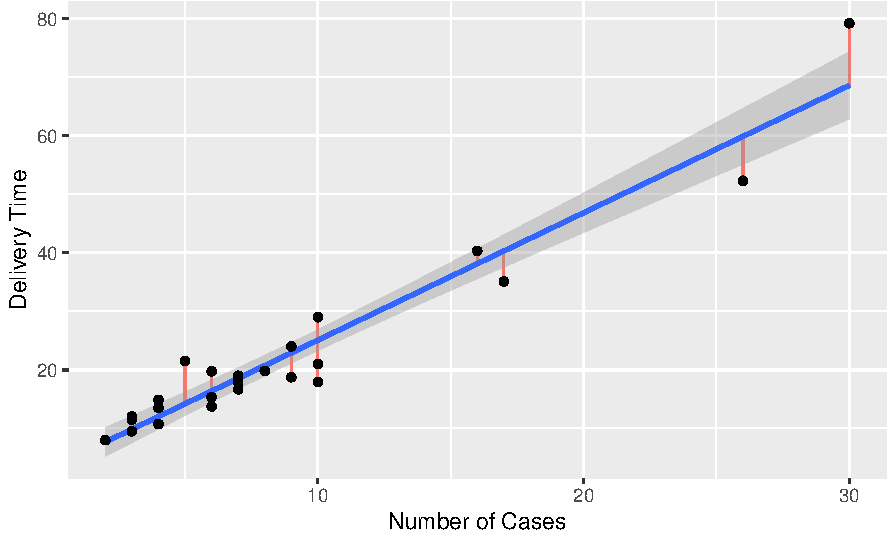
\includegraphics[width=0.7\linewidth]{regression-analysis_files/figure-latex/linassume-1} 

}

\caption{Linearity assumption}\label{fig:linassume}
\end{figure}

\hypertarget{errassumption}{%
\subsection{Errors}\label{errassumption}}

Error term \(\E\) is assumed as

\[\epsilon_i \stackrel{iid}{\sim}N(0, \sigma^2)\]

This involves the following assumptions.

\begin{enumerate}
\def\labelenumi{\arabic{enumi}.}
\tightlist
\item
  \textbf{Mean-zero assumption}: \(\epsilon_i\) has zero mean.
\item
  \textbf{Homoskedasticity} (or homogeneity): \(\epsilon_i\) has constant variance. If variance varies according to observation, we call it as \emph{heteroskedasticity} (or heterogeneity).
\item
  \textbf{Independence assumption}: \(\epsilon_i\) is mutually independent.
\item
  \textbf{Normality assumption}: \(\epsilon_i\) follows Normal distribution.
\end{enumerate}

As mentioned many times, \(\epsilon_j\) cannot be observed. Instead, we gain information from \textbf{residuals}.

\begin{Shaded}
\begin{Highlighting}[]
\NormalTok{delv }\OperatorTok\StringTok{ }
\StringTok{  }\KeywordTok{add_predictions}\NormalTok{(delv_fit) }\OperatorTok\StringTok{ }
\StringTok{  }\KeywordTok{add_residuals}\NormalTok{(delv_fit) }\OperatorTok\StringTok{ }
\StringTok{  }\KeywordTok{ggplot}\NormalTok{(}\KeywordTok{aes}\NormalTok{(}\DataTypeTok{x =}\NormalTok{ pred, }\DataTypeTok{y =}\NormalTok{ resid)) }\OperatorTok{+}
\StringTok{  }\KeywordTok{geom_ref_line}\NormalTok{(}\DataTypeTok{h =} \DecValTok{0}\NormalTok{) }\OperatorTok{+}
\StringTok{  }\KeywordTok{geom_linerange}\NormalTok{(}\KeywordTok{aes}\NormalTok{(}\DataTypeTok{ymin =}\NormalTok{ resid, }\DataTypeTok{ymax =} \DecValTok{0}\NormalTok{), }\DataTypeTok{col =} \KeywordTok{gg_hcl}\NormalTok{(}\DecValTok{1}\NormalTok{), }\DataTypeTok{linetype =} \StringTok{"dotted"}\NormalTok{) }\OperatorTok{+}
\StringTok{  }\KeywordTok{geom_point}\NormalTok{()}
\end{Highlighting}
\end{Shaded}

\begin{figure}[H]

{\centering 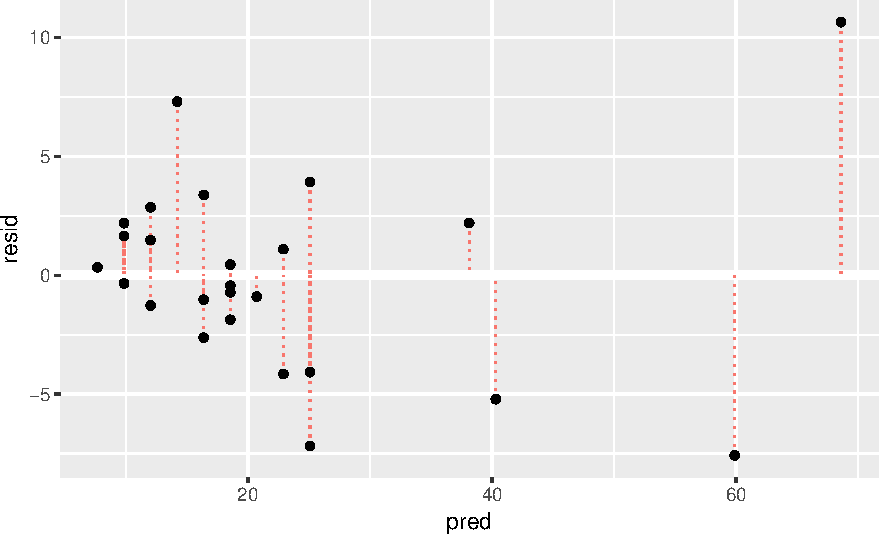
\includegraphics[width=0.7\linewidth]{regression-analysis_files/figure-latex/rsdassume-1} 

}

\caption{Residual plot preview - Does this model satisfy the assumptions?}\label{fig:rsdassume}
\end{figure}

\hypertarget{xassumption}{%
\subsection{Predictors}\label{xassumption}}

\begin{itemize}
\tightlist
\item
  \textbf{Non-random}: While \(Y\) is random variable, \(X_1, \ldots, X_p\) are not. They are assumed fixed or conditioned, i.e.~\(E(Y \mid \mathbf{X} = \mathbf{x})\).
\item
  \textbf{measured without error}: We assume here that \(x_{i1}, \ldots, x_{ip}\) are measured without error, i.e.~there is \emph{no measurement error}. If there is, the measurement error will affect every residual variance, regression coefficient, et cetera. Let \(w_i\) be the measurement error of \(i\)-th observation. Then what we observe is \(Z_i = x_i + w_i\), not \(x_i\). In turn, we estimate regression coefficient and the others using \((Z_i, Y_i)\), i.e.~relationship between \(Z_i\) and \(Y_i\). \emph{Residual variance will increase by construction}. Additionaly, correlation coefficients will be reduced.

  \begin{itemize}
  \tightlist
  \item
    We have assumed that there is no measurement error, but we already know that \emph{it is hardly not true}.
  \item
    So correction for the errors can be considered. But it requires the ratio between \(Var(w_i)\) and \(Var(\epsilon_i)\), which we seldomly know.
  \item
    As a result, we just sacrifice some accuracy for impossible correcting task.
  \end{itemize}
\item
  \textbf{Linear independence}: A set of predictor variables \(\{ X_1, \ldots, X_p \}\) is linearly independent. Recall Theorem \ref{thm:fullrank2}. This makes the design matrix full rank and guarantee unique least squares solution. This is violated by so-called \emph{multicollinearity} problem.
\end{itemize}

First two assumptions cannot be validated, but should be always remembered in the interpretation of the analysis results.

\hypertarget{obsassumption}{%
\subsection{Observations}\label{obsassumption}}

Every observation is equally reliable and plays an equal role in determining the results. When we estimate mean, for instance, each \(X_1, \ldots, X_n\) has equal role so that

\[\hat\mu = \frac{1}{n} X_1 + \cdots + \frac{1}{n} X_n = \overline{X}\]

\begin{figure}[H]

{\centering 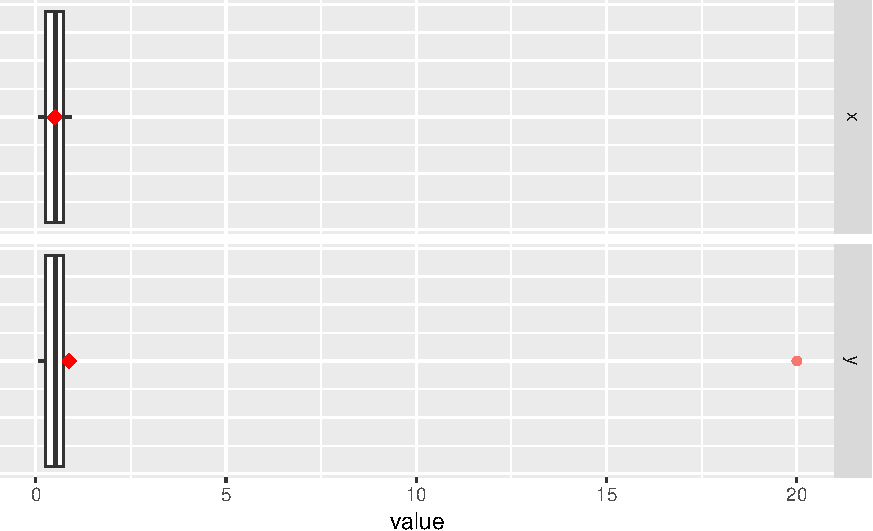
\includegraphics[width=0.7\linewidth]{regression-analysis_files/figure-latex/outassume-1} 

}

\caption{Existence of Outlier}\label{fig:outassume}
\end{figure}

However, if there exists \emph{outlier}, it can be changed critically. See Figure \ref{fig:outassume}. In lower box plot, just one outlier is added: \texttt{20}. Each red dot is average. Thus, we should be careful about \emph{outliers}. In regression literature, we would see the following observations.

\begin{itemize}
\tightlist
\item
  Leverage point
\item
  Influential point
\end{itemize}

\hypertarget{residuals-1}{%
\section{Residuals}\label{residuals-1}}

\hypertarget{raw-residual}{%
\subsection{Raw residual}\label{raw-residual}}

Looking at \(\epsilon_i\), we might be able to check if the model violates the assumptions directly in section \ref{linassumption} and \ref{errassumption}. The problem is \(\epsilon_i\) is non-observable. So as a surrogate, we use residuals

\begin{equation}
  e_i := Y_i - \hat{Y_i} = Y_i - (\hat\beta_0 + \hat\beta_1 x_{i1} + \cdots + \hat\beta_p x_{ip}), \quad i = 1, \ldots, n
  \label{eq:residualdef}
\end{equation}

We already know that \texttt{residuals(model)} or \texttt{model\$residuals} gives residuals. \texttt{modelr::add\_residuals(model)}, additionaly, mutates a colum named \texttt{resid} by default. We can change its name with \texttt{var} argument. See Figure \ref{fig:rsdassume} and its code.

Let

\[\mathbf{e} := (e_1, \ldots, e_p)^T\]

From Proposition \ref{prp:multresprop},

\[\mathbf{e} \sim N(\mathbf{0}, \sigma^2(I - H_X)), \quad H_X = \text{projection onto}\: R(X)\]

This implies that

\[Var(e_i) = (1 - h_{ii})\sigma^2\]

where \(h_{ii}\) is the \(i\)-th diagonal element of \(H_X\). Recall that

\[Var(\epsilon_i) = \sigma^2\]

As a backup of \(\sigma^2\), \(e_i\) should reflect the assumption of \(\epsilon_i\). \emph{Scaling} might be needed.

\hypertarget{standardized-residual}{%
\subsection{Standardized residual}\label{standardized-residual}}

Applying usual standardization procedure, one may use

\begin{equation}
  e_i^{\ast} = \frac{e_i}{\sigma \sqrt{1 - h_{ii}}}
  \label{eq:stdunknown}
\end{equation}

\(\sigma\) is unkown. So replace \(\sigma\) with \(\hat\sigma\).

\BeginKnitrBlock{definition}[Standardized residual]
\protect\hypertarget{def:stdresid}{}{\label{def:stdresid} \iffalse (Standardized residual) \fi{} }Standardized residual can be obtained by replacing \(\sigma\) with \(\hat\sigma\).

\[d_i := \frac{e_i}{\hat\sigma \sqrt{1 - h_{ii}}}\]

where \(\hat\sigma^2 = \frac{\sum\limits_{i = 1}^n e_i^2}{n - p - 1}\).
\EndKnitrBlock{definition}

We can get values of \(d_i\) with \texttt{rstandard()}.

\begin{Shaded}
\begin{Highlighting}[]
\KeywordTok{rstandard}\NormalTok{(delv_fit)}
\CommentTok{#>       1       2       3       4       5       6       7       8       9 }
\CommentTok{#> -0.4581  0.4092  0.5406  0.7041 -0.6437 -0.1085  0.0815 -0.1770  3.3893 }
\CommentTok{#>      10      11      12      13      14      15      16      17      18 }
\CommentTok{#>  1.7931  0.5480 -0.9972  0.3637  0.8260  0.2670  0.9569 -0.2517  0.1090 }
\CommentTok{#>      19      20      21      22      23      24      25 }
\CommentTok{#> -0.0866 -1.3146 -1.7544 -2.1694 -1.0145 -0.2198 -0.3146}
\end{Highlighting}
\end{Shaded}

In fact, we can get both residuals using \texttt{broom::augment()}.

\begin{itemize}
\tightlist
\item
  \texttt{.fitted}: fitted values
\item
  \texttt{.resid}: raw residuals
\item
  \texttt{.std.resid}: standardized residuals
\end{itemize}

\begin{Shaded}
\begin{Highlighting}[]
\NormalTok{delv_fit }\OperatorTok\StringTok{ }
\StringTok{  }\NormalTok{broom}\OperatorTok{::}\KeywordTok{augment}\NormalTok{() }\OperatorTok\StringTok{ }
\StringTok{  }\KeywordTok{gather}\NormalTok{(.resid, .std.resid, }\DataTypeTok{key =} \StringTok{"residual"}\NormalTok{, }\DataTypeTok{value =} \StringTok{"value"}\NormalTok{) }\OperatorTok\StringTok{ }
\StringTok{  }\KeywordTok{ggplot}\NormalTok{(}\KeywordTok{aes}\NormalTok{(}\DataTypeTok{x =}\NormalTok{ .fitted, }\DataTypeTok{y =}\NormalTok{ value, }\DataTypeTok{colour =}\NormalTok{ residual)) }\OperatorTok{+}
\StringTok{  }\KeywordTok{geom_ref_line}\NormalTok{(}\DataTypeTok{h =} \DecValTok{0}\NormalTok{) }\OperatorTok{+}
\StringTok{  }\KeywordTok{geom_linerange}\NormalTok{(}\KeywordTok{aes}\NormalTok{(}\DataTypeTok{ymin =}\NormalTok{ value, }\DataTypeTok{ymax =} \DecValTok{0}\NormalTok{), }\DataTypeTok{linetype =} \StringTok{"dotted"}\NormalTok{) }\OperatorTok{+}
\StringTok{  }\KeywordTok{geom_point}\NormalTok{() }\OperatorTok{+}
\StringTok{  }\KeywordTok{labs}\NormalTok{(}
    \DataTypeTok{y =} \StringTok{"Residuals"}\NormalTok{,}
    \DataTypeTok{x =} \StringTok{"Prediction"}
\NormalTok{  ) }\OperatorTok{+}
\StringTok{  }\KeywordTok{scale_colour_discrete}\NormalTok{(}
    \DataTypeTok{name =} \StringTok{"Residuals"}\NormalTok{,}
    \DataTypeTok{label =} \KeywordTok{c}\NormalTok{(}\StringTok{"Raw"}\NormalTok{, }\StringTok{"Std"}\NormalTok{)}
\NormalTok{  )}
\end{Highlighting}
\end{Shaded}

\begin{figure}[H]

{\centering 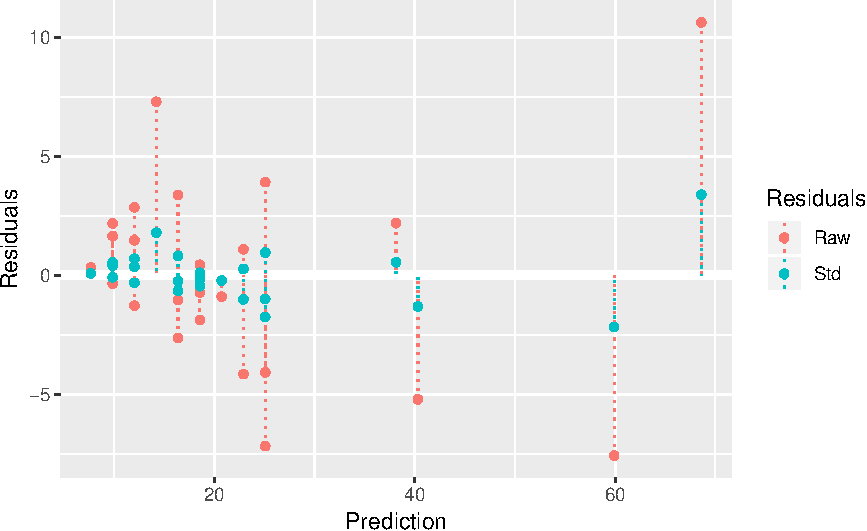
\includegraphics[width=0.7\linewidth]{regression-analysis_files/figure-latex/rstdresid-1} 

}

\caption{Standardized residuals}\label{fig:rstdresid}
\end{figure}

Does this \(d_i\) follow \(t(n - p - 1)\)? \(Z := \frac{e_i}{\sigma \sqrt{1 - h_{ii}}} \sim N(0, 1)\) and \(X := \frac{\hat\sigma}{\sigma} \sim \chi^2(n - p - 1)\). In the other context, this typically leads to \(t\)-distribution. Here, however, \(Z\) and \(X\) are not independent. Denote that \(\hat\sigma^2 = \frac{\sum\limits_{i = 1}^n e_i^2}{n - p - 1}\) includes \(e_i\), so it cannot be independent with \(e_i\). Thus, \(d_i\) is not \(t\) distributed.

\hypertarget{studentized-residual}{%
\subsection{Studentized residual}\label{studentized-residual}}

To force \(d_i\) to be \(t\) random variable, we just prevent from each \(e_i\) encountering each \(e_i\) in \(\hat\sigma^2\). This can be done by computing MSE without \(i\)-th observation, i.e.~using data set

\[
D_{(-i)} := \begin{bmatrix}
  (\mathbf{x}_1, Y_1) \\
  (\mathbf{x}_2, Y_2) \\
  \vdots \\
  \msout{(\mathbf{x}_i, Y_i)} \\
  \vdots \\
  (\mathbf{x}_n, Y_n)
\end{bmatrix}
\]

compute MSE \(\hat\sigma_{(-i)}^2\).

\BeginKnitrBlock{definition}[Studentized residual]
\protect\hypertarget{def:studresid}{}{\label{def:studresid} \iffalse (Studentized residual) \fi{} }The studentized residual is defined by

\[r_i := \frac{e_i}{\hat\sigma_{(-i)} \sqrt{1 - h_{ii}}}\]

where \(\hat\sigma_{(-i)}^2\) is MSE from data without \(i\)-th observation, \(D_{(-i)}\).
\EndKnitrBlock{definition}

In principle, we need to fit \(n\) different models to get this residuals. In fact, this is not necessary because \(\hat\sigma_{(-i)}^2\) has some relation to \(\hat\sigma^2\).

\BeginKnitrBlock{lemma}
\protect\hypertarget{lem:studsig}{}{\label{lem:studsig} }\(\hat\sigma_{(-i)}^2\) can be computed from the original \(\hat\sigma^2\).

\[\hat\sigma_{(-i)}^2 = \frac{(n - p - 1)\hat\sigma^2 - \frac{e_i^2}{1 - h_{ii}}}{n - p - 1}\]
\EndKnitrBlock{lemma}

This lemma removes repeating procedure.

\BeginKnitrBlock{corollary}
\protect\hypertarget{cor:unnamed-chunk-125}{}{\label{cor:unnamed-chunk-125} }Studentized residuals and standardized residuals are related by

\[r_i = d_i \frac{n - p - 2}{n - p - 1 - d_i^2}\]

where \(d_i\) are standardized residuals and \(r_i\) are studentized residuals.
\EndKnitrBlock{corollary}

\texttt{rstudent()} gives this \(r_i\) in \texttt{R}.

\begin{Shaded}
\begin{Highlighting}[]
\KeywordTok{rstudent}\NormalTok{(delv_fit)}
\CommentTok{#>       1       2       3       4       5       6       7       8       9 }
\CommentTok{#> -0.4500  0.4017  0.5321  0.6962 -0.6353 -0.1062  0.0797 -0.1732  4.6851 }
\CommentTok{#>      10      11      12      13      14      15      16      17      18 }
\CommentTok{#>  1.8908  0.5395 -0.9970  0.3567  0.8201  0.2615  0.9551 -0.2466  0.1067 }
\CommentTok{#>      19      20      21      22      23      24      25 }
\CommentTok{#> -0.0847 -1.3369 -1.8436 -2.3790 -1.0152 -0.2152 -0.3084}
\end{Highlighting}
\end{Shaded}

\begin{Shaded}
\begin{Highlighting}[]
\CommentTok{# n = 25}
\CommentTok{# p = 1}
\KeywordTok{rstandard}\NormalTok{(delv_fit) }\OperatorTok{*}\StringTok{ }\KeywordTok{sqrt}\NormalTok{((}\DecValTok{25} \OperatorTok{-}\StringTok{ }\DecValTok{3}\NormalTok{) }\OperatorTok{/}\StringTok{ }\NormalTok{(}\DecValTok{25} \OperatorTok{-}\StringTok{ }\DecValTok{2} \OperatorTok{-}\StringTok{ }\KeywordTok{rstandard}\NormalTok{(delv_fit)}\OperatorTok{^}\DecValTok{2}\NormalTok{))}
\CommentTok{#>       1       2       3       4       5       6       7       8       9 }
\CommentTok{#> -0.4500  0.4017  0.5321  0.6962 -0.6353 -0.1062  0.0797 -0.1732  4.6851 }
\CommentTok{#>      10      11      12      13      14      15      16      17      18 }
\CommentTok{#>  1.8908  0.5395 -0.9970  0.3567  0.8201  0.2615  0.9551 -0.2466  0.1067 }
\CommentTok{#>      19      20      21      22      23      24      25 }
\CommentTok{#> -0.0847 -1.3369 -1.8436 -2.3790 -1.0152 -0.2152 -0.3084}
\end{Highlighting}
\end{Shaded}

\texttt{broom::(augment)} does not provide \texttt{rstudent()} yet, so here \texttt{mutate} them all in hand.

\begin{Shaded}
\begin{Highlighting}[]
\NormalTok{delv }\OperatorTok\StringTok{ }
\StringTok{  }\KeywordTok{add_predictions}\NormalTok{(delv_fit) }\OperatorTok\StringTok{ }
\StringTok{  }\KeywordTok{mutate}\NormalTok{(}
    \DataTypeTok{resid =} \KeywordTok{residuals}\NormalTok{(delv_fit),}
    \DataTypeTok{std =} \KeywordTok{rstandard}\NormalTok{(delv_fit),}
    \DataTypeTok{stud =} \KeywordTok{rstudent}\NormalTok{(delv_fit)}
\NormalTok{  ) }\OperatorTok\StringTok{ }
\StringTok{  }\KeywordTok{gather}\NormalTok{(resid, std, stud, }\DataTypeTok{key =} \StringTok{"residual"}\NormalTok{, }\DataTypeTok{value =} \StringTok{"value"}\NormalTok{) }\OperatorTok\StringTok{ }
\StringTok{  }\KeywordTok{ggplot}\NormalTok{(}\KeywordTok{aes}\NormalTok{(}\DataTypeTok{x =}\NormalTok{ pred, }\DataTypeTok{y =}\NormalTok{ value, }\DataTypeTok{colour =}\NormalTok{ residual)) }\OperatorTok{+}
\StringTok{  }\KeywordTok{geom_ref_line}\NormalTok{(}\DataTypeTok{h =} \DecValTok{0}\NormalTok{) }\OperatorTok{+}
\StringTok{  }\KeywordTok{geom_linerange}\NormalTok{(}\KeywordTok{aes}\NormalTok{(}\DataTypeTok{ymin =}\NormalTok{ value, }\DataTypeTok{ymax =} \DecValTok{0}\NormalTok{), }\DataTypeTok{linetype =} \StringTok{"dotted"}\NormalTok{) }\OperatorTok{+}
\StringTok{  }\KeywordTok{geom_point}\NormalTok{() }\OperatorTok{+}
\StringTok{  }\KeywordTok{labs}\NormalTok{(}
    \DataTypeTok{y =} \StringTok{"Residuals"}\NormalTok{,}
    \DataTypeTok{x =} \StringTok{"Prediction"}
\NormalTok{  ) }\OperatorTok{+}
\StringTok{  }\KeywordTok{scale_colour_discrete}\NormalTok{(}
    \DataTypeTok{name =} \StringTok{"Residuals"}\NormalTok{,}
    \DataTypeTok{label =} \KeywordTok{c}\NormalTok{(}\StringTok{"Raw"}\NormalTok{, }\StringTok{"Std"}\NormalTok{, }\StringTok{"Student"}\NormalTok{)}
\NormalTok{  )}
\end{Highlighting}
\end{Shaded}

\begin{figure}[H]

{\centering 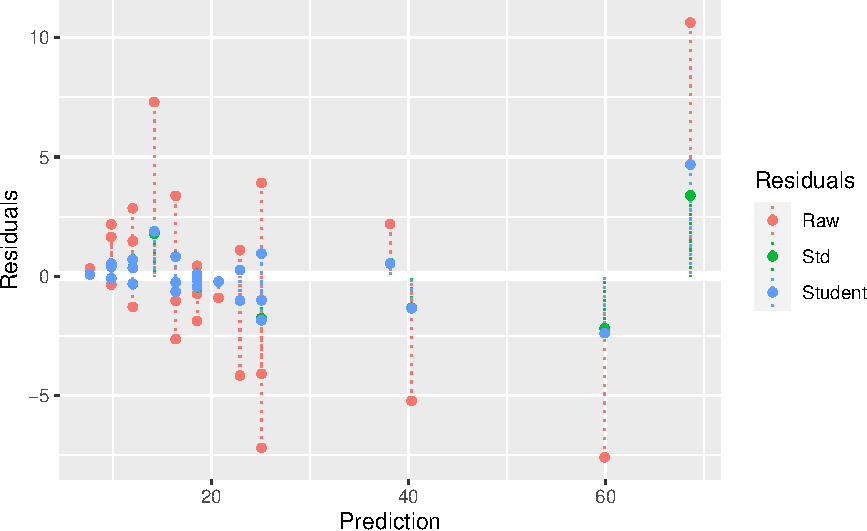
\includegraphics[width=0.7\linewidth]{regression-analysis_files/figure-latex/rstudresid-1} 

}

\caption{Studentized residuals}\label{fig:rstudresid}
\end{figure}

\citet{Chatterjee:2015aa} names the above three \eqref{eq:stdunknown} \(e_i^{\ast}\), \ref{def:stdresid} \(d_i\), and \ref{def:studresid} \(r_i\) as follows.

\BeginKnitrBlock{remark}
\iffalse{} {Remark. } \fi{}The form of residual in Equation \eqref{eq:stdunknown}, Definition \ref{def:stdresid}, and \ref{def:studresid} can be called as

\begin{enumerate}
  \item $e_i^{\ast} := \frac{e_i}{\sigma \sqrt{1 - h_{ii}}}$ \textit{Standardized residual}
  \item $d_i := \frac{e_i}{\hat\sigma \sqrt{1 - h_{ii}}}$ \textit{Internally studentized residual}
  \item $r_i := \frac{e_i}{\hat\sigma_{(-i)} \sqrt{1 - h_{ii}}}$ \textit{Externally studentized residual}
\end{enumerate}
\EndKnitrBlock{remark}

The word \emph{internal} and \emph{external} is due to direct involvement of \(\hat\sigma\) in \(e_i\). In externally studentized residual, \(\hat\sigma_{(-i)}\) is not involved in \(e_i\), i.e.~external to \(e_i\).

\hypertarget{residual-plots}{%
\section{Residual Plots}\label{residual-plots}}

Graphical methods are able to become some kind of caveat. It is effective way to investigate model adequacy.

\begin{Shaded}
\begin{Highlighting}[]
\NormalTok{gg_fit <-}\StringTok{ }\ControlFlowTok{function}\NormalTok{(data, mapping) \{}
\NormalTok{  pt <-}\StringTok{ }\KeywordTok{gg_scatter}\NormalTok{(data, }\DataTypeTok{mapping =}\NormalTok{ mapping, }\DataTypeTok{alpha =} \DecValTok{1}\NormalTok{)}
\NormalTok{  pt}\OperatorTok{$}\NormalTok{layers <-}\StringTok{ }\KeywordTok{c}\NormalTok{(}\KeywordTok{geom_smooth}\NormalTok{(}\DataTypeTok{method =} \StringTok{"lm"}\NormalTok{), pt}\OperatorTok{$}\NormalTok{layers)}
\NormalTok{  pt }\CommentTok{# point layer on line layer}
\NormalTok{\}}
\CommentTok{#------------------------------------}
\NormalTok{draw_dot <-}\StringTok{ }\ControlFlowTok{function}\NormalTok{(data, mapping, ...) \{}
\NormalTok{  data }\OperatorTok\StringTok{ }
\StringTok{    }\KeywordTok{ggplot}\NormalTok{(}\DataTypeTok{mapping =}\NormalTok{ mapping) }\OperatorTok{+}
\StringTok{    }\KeywordTok{geom_dotplot}\NormalTok{(...)}
\NormalTok{\}}
\end{Highlighting}
\end{Shaded}

Since \texttt{gg\_scatter()} is pre-defined function drawing a scatter plot, we can change the order of layers by indexing its \texttt{layers}. This is because every \texttt{geom\_*} and \texttt{stat\_*} returns \texttt{layer()}. For example,

\begin{Shaded}
\begin{Highlighting}[]
\NormalTok{geom_smooth}
\CommentTok{#> function (mapping = NULL, data = NULL, stat = "smooth", position = "identity", }
\CommentTok{#>     ..., method = "auto", formula = y ~ x, se = TRUE, na.rm = FALSE, }
\CommentTok{#>     show.legend = NA, inherit.aes = TRUE) }
\CommentTok{#> \{}
\CommentTok{#>     params <- list(na.rm = na.rm, se = se, ...)}
\CommentTok{#>     if (identical(stat, "smooth")) \{}
\CommentTok{#>         params$method <- method}
\CommentTok{#>         params$formula <- formula}
\CommentTok{#>     \}}
\CommentTok{#>     layer(data = data, mapping = mapping, stat = stat, geom = GeomSmooth, }
\CommentTok{#>         position = position, show.legend = show.legend, inherit.aes = inherit.aes, }
\CommentTok{#>         params = params)}
\CommentTok{#> \}}
\CommentTok{#> <bytecode: 0x7f95790e2dd0>}
\CommentTok{#> <environment: namespace:ggplot2>}
\end{Highlighting}
\end{Shaded}

\texttt{GGally::ggpairs()} easily draws a matrix of plots. We can specify each \texttt{lower}, \texttt{upper}, and \texttt{diag}.

\begin{Shaded}
\begin{Highlighting}[]
\NormalTok{cem }\OperatorTok\StringTok{ }
\StringTok{  }\NormalTok{GGally}\OperatorTok{::}\KeywordTok{ggpairs}\NormalTok{(}
    \DataTypeTok{lower =} \KeywordTok{list}\NormalTok{(}\DataTypeTok{continuous =}\NormalTok{ gg_fit), }\CommentTok{# regression}
    \DataTypeTok{diag =} \KeywordTok{list}\NormalTok{(}\DataTypeTok{continuous =}\NormalTok{ draw_dot) }\CommentTok{# dot plot}
\NormalTok{  )}
\end{Highlighting}
\end{Shaded}

\begin{figure}[H]

{\centering 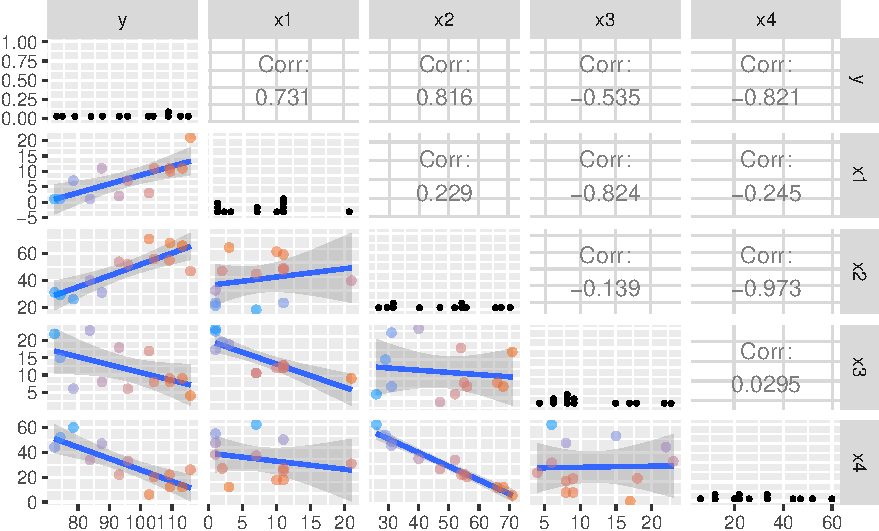
\includegraphics[width=0.7\linewidth]{regression-analysis_files/figure-latex/plmat-1} 

}

\caption{Plot matrix for cement data set}\label{fig:plmat}
\end{figure}

Plots that have scatter plot in the matrix form and pairwise correlation such as Figure \ref{fig:plmat} is called \emph{plot matrix} or \emph{scatter matrix}. First column let us know the relationship between \texttt{y} and each \texttt{x}. Correlation is important in that we have assumed linear independence. This would be covered later.

\hypertarget{residual-plot}{%
\subsection{Residual plot}\label{residual-plot}}

Direct illustration of \(Y\) and \(X_1, \ldots, X_p\) is helpful, but has its limit to check the assumptions. Residuals might be more informative. Among the three we have defined, we often draw \emph{externally studentized residual} \ref{def:studresid}, i.e.~\texttt{rstudent()}.

\[r_i := \frac{e_i}{\hat\sigma_{(-i)} \sqrt{1 - h_{ii}}}\]

\BeginKnitrBlock{definition}[Residual plot]
\protect\hypertarget{def:residplot}{}{\label{def:residplot} \iffalse (Residual plot) \fi{} }Residual plot is a plot of \(r_i\) versus corresponding fitted values \(\hat{Y_i}\)
\EndKnitrBlock{definition}

In \texttt{modelr} syntax,

\begin{Shaded}
\begin{Highlighting}[]
\NormalTok{add_rstudent <-}\StringTok{ }\ControlFlowTok{function}\NormalTok{(data, model, }\DataTypeTok{var =} \StringTok{".stud.resid"}\NormalTok{) \{}
\NormalTok{  data[[var]] <-}\StringTok{ }\KeywordTok{rstudent}\NormalTok{(model, }\DataTypeTok{x =}\NormalTok{ data)}
\NormalTok{  data}
\NormalTok{\}}
\CommentTok{#----------------------------------------}
\NormalTok{residplot <-}\StringTok{ }\ControlFlowTok{function}\NormalTok{(data, model, ...) \{}
\NormalTok{  data }\OperatorTok\StringTok{ }
\StringTok{    }\KeywordTok{add_predictions}\NormalTok{(model) }\OperatorTok\StringTok{ }
\StringTok{    }\KeywordTok{add_rstudent}\NormalTok{(model) }\OperatorTok\StringTok{ }
\StringTok{    }\KeywordTok{ggplot}\NormalTok{(data, }\DataTypeTok{mapping =} \KeywordTok{aes}\NormalTok{(}\DataTypeTok{x =}\NormalTok{ pred, }\DataTypeTok{y =}\NormalTok{ .stud.resid)) }\OperatorTok{+}
\StringTok{    }\KeywordTok{geom_ref_line}\NormalTok{(}\DataTypeTok{h =} \DecValTok{0}\NormalTok{) }\OperatorTok{+}
\StringTok{    }\KeywordTok{geom_point}\NormalTok{(...)}
\NormalTok{\}}
\end{Highlighting}
\end{Shaded}

\begin{Shaded}
\begin{Highlighting}[]
\KeywordTok{residplot}\NormalTok{(cem, cem_fit) }\OperatorTok{+}
\StringTok{  }\KeywordTok{labs}\NormalTok{(}
    \DataTypeTok{x =} \StringTok{"Fitted values"}\NormalTok{,}
    \DataTypeTok{y =} \StringTok{"Residuals"}
\NormalTok{  )}
\end{Highlighting}
\end{Shaded}

\begin{figure}[H]

{\centering 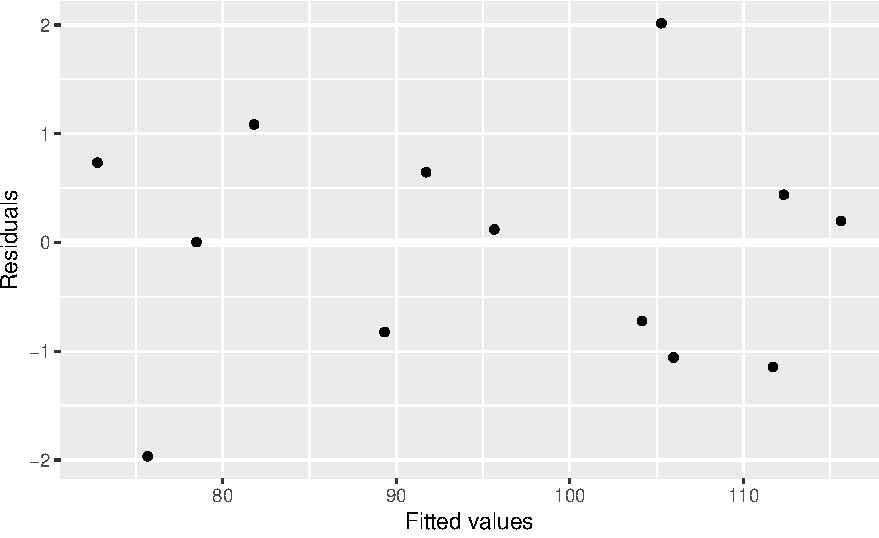
\includegraphics[width=0.7\linewidth]{regression-analysis_files/figure-latex/cemrsplot-1} 

}

\caption{Residual plot for regression with cement data set}\label{fig:cemrsplot}
\end{figure}

Denote that

\[r_i \stackrel{iid}{\approx} N(0, 1)\]

So we can deduct some ideal behavior of \(r_i\).

\BeginKnitrBlock{remark}
\iffalse{} {Remark. } \fi{}Ideally, residual plot should be

\begin{itemize}
  \item have \textit{no systematic pattern}
  \item equal variance, i.e. \textit{variability of} $r_i$ \textit{shows constancy}, independent of $\hat{Y_i}$
  \item most $r_i$s fall between $-2$ and $2$, approximately $95\%$
\end{itemize}
\EndKnitrBlock{remark}

Now consider various scenarios and see how to interpret this plot.

\begin{Shaded}
\begin{Highlighting}[]
\KeywordTok{residplot}\NormalTok{(hetero, hetero_fit)}
\end{Highlighting}
\end{Shaded}

\begin{figure}[H]

{\centering 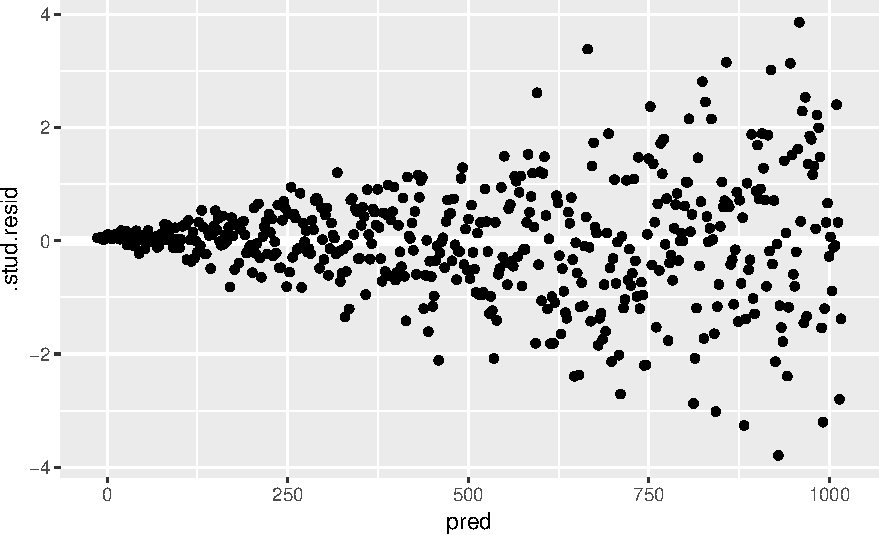
\includegraphics[width=0.7\linewidth]{regression-analysis_files/figure-latex/heteropt-1} 

}

\caption{Heteroskedasticity}\label{fig:heteropt}
\end{figure}

As \(i\) grows, variance becomes larger. Constant variance assumption is violated.

\begin{Shaded}
\begin{Highlighting}[]
\KeywordTok{residplot}\NormalTok{(cubic, cubic_fit)}
\end{Highlighting}
\end{Shaded}

\begin{figure}[H]

{\centering 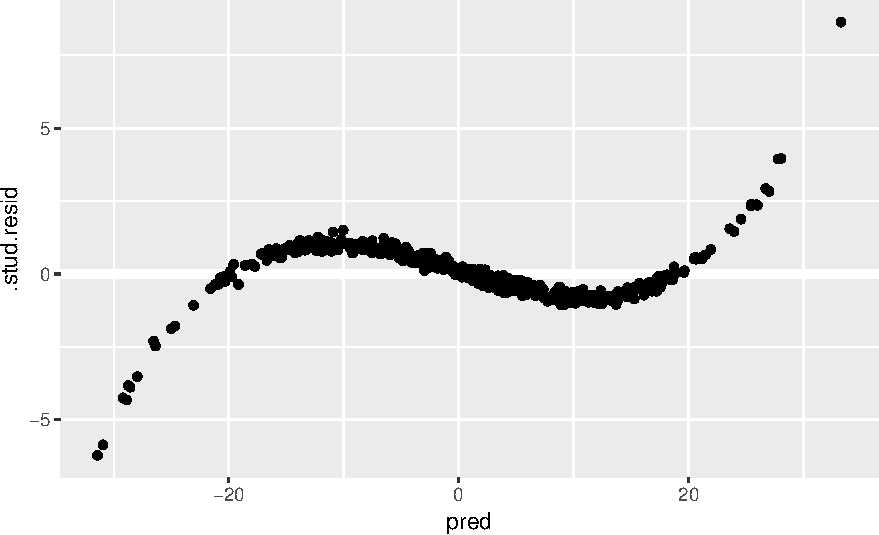
\includegraphics[width=0.7\linewidth]{regression-analysis_files/figure-latex/nonlinpt-1} 

}

\caption{Non-linear relationship and autocorrelation}\label{fig:nonlinpt}
\end{figure}

By its definition, residuals are values after removing linear effects. If the data embeds non-linear relationships, it would not be removed and it would be still remained as pattern. Figure \ref{fig:nonlinpt} indicates that \(Y\) and \(x\) have non-linear relationship.

\begin{Shaded}
\begin{Highlighting}[]
\KeywordTok{residplot}\NormalTok{(outlier, outlier_fit) }\OperatorTok{+}
\StringTok{  }\KeywordTok{geom_point}\NormalTok{(}\KeywordTok{aes}\NormalTok{(}\DataTypeTok{colour =}\NormalTok{ isout), }\DataTypeTok{na.rm =} \OtherTok{TRUE}\NormalTok{, }\DataTypeTok{shape =} \DecValTok{1}\NormalTok{, }\DataTypeTok{size =} \DecValTok{3}\NormalTok{, }\DataTypeTok{show.legend =} \OtherTok{FALSE}\NormalTok{) }\OperatorTok{+}
\StringTok{  }\KeywordTok{scale_colour_manual}\NormalTok{(}\DataTypeTok{values =} \KeywordTok{c}\NormalTok{(}\StringTok{"TRUE"}\NormalTok{ =}\StringTok{ "red"}\NormalTok{, }\StringTok{"FALSE"}\NormalTok{ =}\StringTok{ }\OtherTok{NA}\NormalTok{))}
\end{Highlighting}
\end{Shaded}

\begin{figure}[H]

{\centering 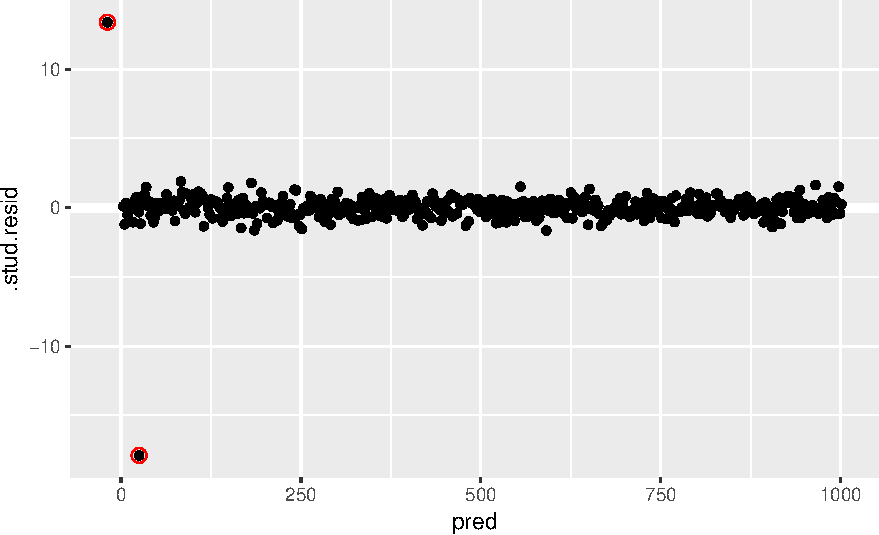
\includegraphics[width=0.7\linewidth]{regression-analysis_files/figure-latex/outpt-1} 

}

\caption{Existence of outlier}\label{fig:outpt}
\end{figure}

Large values of residuals implies they are outliers.

\hypertarget{normal-quantile-quantile-plot}{%
\subsection{Normal quantile-quantile plot}\label{normal-quantile-quantile-plot}}

We expect that

\[r_i \stackrel{iid}{\sim}N(0, 1)\]

Normal quantile-quantile plot (q-q plot) or normal probability plot can tell us whether observations of \(r_i\) is closed to \emph{Normal distribution}.

\BeginKnitrBlock{definition}[Normal q-q plot]
\protect\hypertarget{def:qqpt}{}{\label{def:qqpt} \iffalse (Normal q-q plot) \fi{} }Normal Q-Q plot is the plot of \textit{ordered studentized residuals} \(r_{(1)} < r_{(2)} < \cdots < r_{(n)}\) versus \textit{theoretical normal quantiles} \(\Phi^{+}\bigg( \frac{i - \frac{3}{8}}{n + \frac{1}{4}} \bigg)\).
\EndKnitrBlock{definition}

\emph{If Q-Q plot is close to a straight line, this supports the Normality of residuals.} Otherwise, we can say that the assumption is violated.

\texttt{ggplot2} provides \texttt{stat\_qq\_line()} and \texttt{stat\_qq()}. One draws the guide line and the other draws a points of q-q plot. There is an argument \texttt{distribution}. We can compare observations with any distribution function. The default, of course, is \texttt{stats::qnorm}, i.e.~normal distribution.

\begin{Shaded}
\begin{Highlighting}[]
\NormalTok{cem }\OperatorTok\StringTok{ }
\StringTok{  }\KeywordTok{add_rstudent}\NormalTok{(cem_fit) }\OperatorTok\StringTok{ }
\StringTok{  }\KeywordTok{ggplot}\NormalTok{(}\KeywordTok{aes}\NormalTok{(}\DataTypeTok{sample =}\NormalTok{ .stud.resid)) }\OperatorTok{+}
\StringTok{  }\KeywordTok{stat_qq_line}\NormalTok{(}
    \DataTypeTok{distribution =}\NormalTok{ stats}\OperatorTok{::}\NormalTok{qnorm,}
    \DataTypeTok{col =} \KeywordTok{I}\NormalTok{(}\StringTok{"white"}\NormalTok{),}
    \DataTypeTok{size =} \DecValTok{2}
\NormalTok{  ) }\OperatorTok{+}
\StringTok{  }\KeywordTok{stat_qq}\NormalTok{(}\DataTypeTok{distribution =}\NormalTok{ stats}\OperatorTok{::}\NormalTok{qnorm)}
\end{Highlighting}
\end{Shaded}

\begin{figure}[H]

{\centering 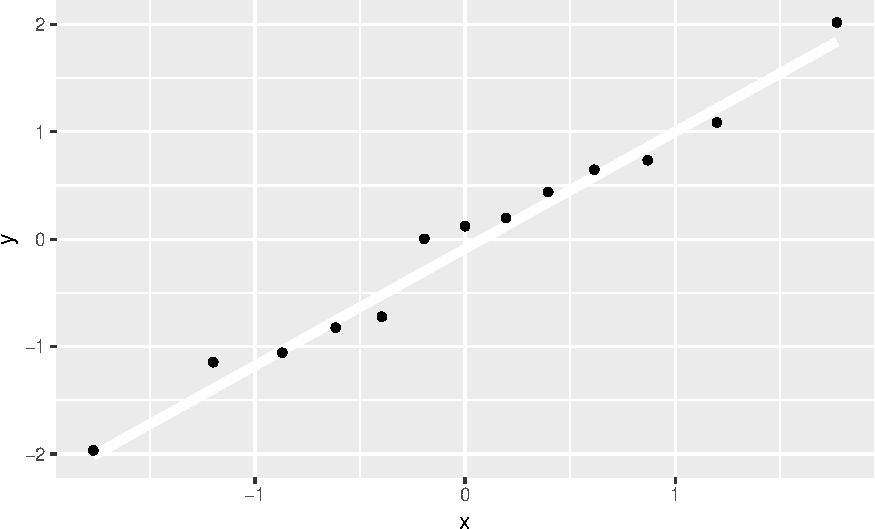
\includegraphics[width=0.7\linewidth]{regression-analysis_files/figure-latex/qqcement-1} 

}

\caption{Q-Q plot for cement residuals}\label{fig:qqcement}
\end{figure}

In general, we filter \emph{skewness} here.

\begin{Shaded}
\begin{Highlighting}[]
\NormalTok{draw_qq <-}\StringTok{ }\ControlFlowTok{function}\NormalTok{(data, model, }\DataTypeTok{distribution =}\NormalTok{ stats}\OperatorTok{::}\NormalTok{qnorm, ...) \{}
\NormalTok{  data }\OperatorTok\StringTok{ }
\StringTok{    }\KeywordTok{add_rstudent}\NormalTok{(model) }\OperatorTok\StringTok{ }
\StringTok{    }\KeywordTok{ggplot}\NormalTok{(}\KeywordTok{aes}\NormalTok{(}\DataTypeTok{sample =}\NormalTok{ .stud.resid)) }\OperatorTok{+}
\StringTok{    }\KeywordTok{stat_qq_line}\NormalTok{(}\DataTypeTok{distribution =}\NormalTok{ distribution, ...) }\OperatorTok{+}
\StringTok{    }\KeywordTok{stat_qq}\NormalTok{(}\DataTypeTok{distribution =}\NormalTok{ distribution) }\OperatorTok{+}
\StringTok{    }\KeywordTok{xlab}\NormalTok{(}\StringTok{"Theoretical Quantiles"}\NormalTok{)}
\NormalTok{\}}
\end{Highlighting}
\end{Shaded}

\begin{Shaded}
\begin{Highlighting}[]
\KeywordTok{draw_qq}\NormalTok{(ideal, ideal_fit, }\DataTypeTok{col =} \KeywordTok{I}\NormalTok{(}\StringTok{"white"}\NormalTok{), }\DataTypeTok{size =} \DecValTok{2}\NormalTok{)}
\end{Highlighting}
\end{Shaded}

\begin{figure}[H]

{\centering 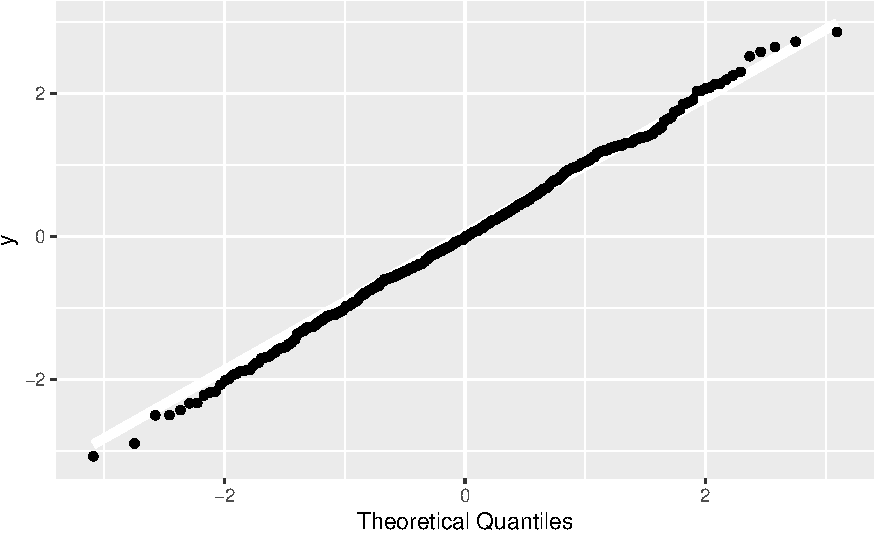
\includegraphics[width=0.7\linewidth]{regression-analysis_files/figure-latex/idqq-1} 

}

\caption{Q-Q plot - Ideal case}\label{fig:idqq}
\end{figure}

Figure \ref{fig:idqq} shows the ideal case. Observations resemble the straight line.

\begin{Shaded}
\begin{Highlighting}[]
\KeywordTok{draw_qq}\NormalTok{(fat, fat_fit, }\DataTypeTok{col =} \KeywordTok{I}\NormalTok{(}\StringTok{"white"}\NormalTok{), }\DataTypeTok{size =} \DecValTok{2}\NormalTok{)}
\end{Highlighting}
\end{Shaded}

\begin{figure}[H]

{\centering 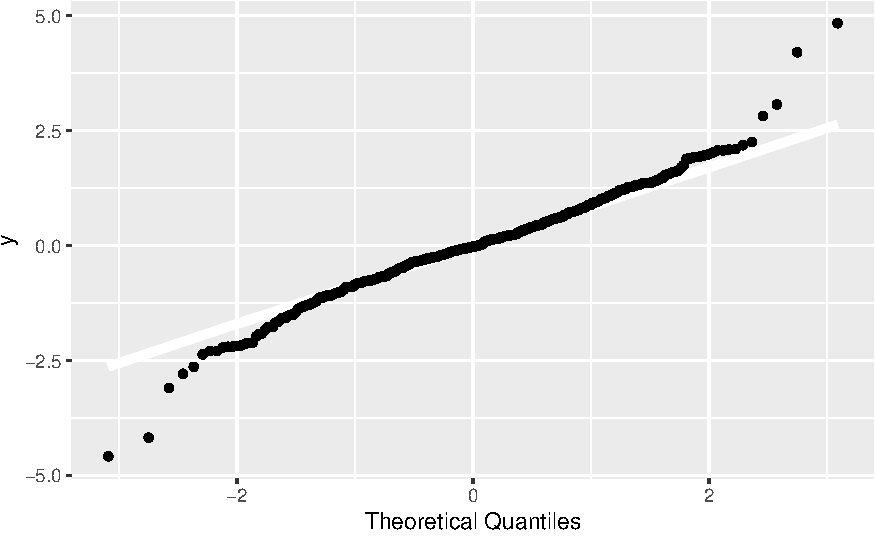
\includegraphics[width=0.7\linewidth]{regression-analysis_files/figure-latex/qqt-1} 

}

\caption{Q-Q plot - Heavy-tailed distribution}\label{fig:qqt}
\end{figure}

Recall that the \(x\)-axis is \emph{theoretical} normal quantile and \(y\)-axis is the \emph{observed} ordered studentized residuals. In case of small values of \(r_i\), i.e.~\emph{left tail}, observed values indicating empirical quantiles are less than theoretical quantiles. \emph{Smaller quantiles at left tail means heavier left tail}. At \emph{right tail}, on the other hand, observed values indicating empirical quantiles are larger than theoretical quantiles. \emph{Larger quantiles at right tail means heavier right tail}. In sum, Figure \ref{fig:qqt} form is of heavy-tailed distribution.

\begin{Shaded}
\begin{Highlighting}[]
\KeywordTok{draw_qq}\NormalTok{(thin, thin_fit, }\DataTypeTok{col =} \KeywordTok{I}\NormalTok{(}\StringTok{"white"}\NormalTok{), }\DataTypeTok{size =} \DecValTok{2}\NormalTok{)}
\end{Highlighting}
\end{Shaded}

\begin{figure}[H]

{\centering 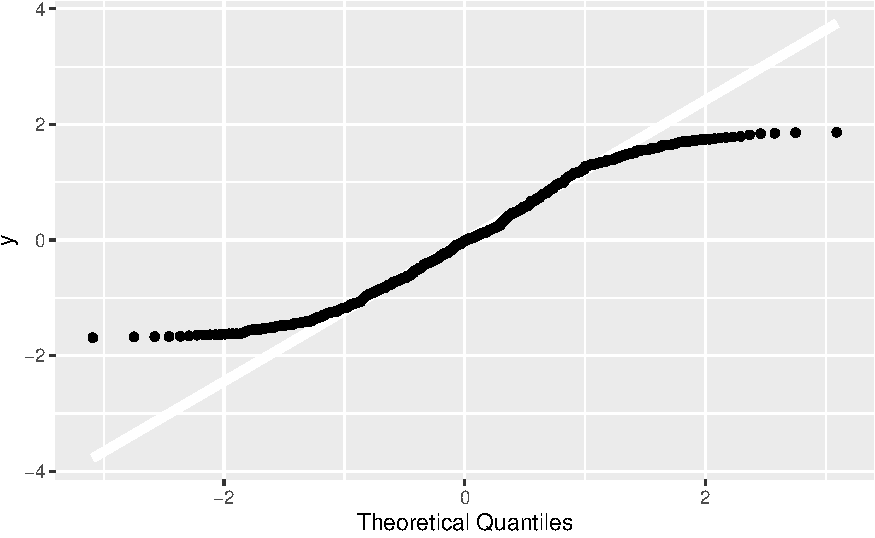
\includegraphics[width=0.7\linewidth]{regression-analysis_files/figure-latex/qqunif-1} 

}

\caption{Q-Q plot - Light-tailed distribution}\label{fig:qqunif}
\end{figure}

This is exactly opposite result with Figure \ref{fig:qqt}. Larger empirical quantiles at left tail implies light left tail. Smaller empirical quantiles at right tail implies light right tail. This is the form of light-tailed distribution.

\begin{Shaded}
\begin{Highlighting}[]
\KeywordTok{draw_qq}\NormalTok{(right, right_fit, }\DataTypeTok{col =} \KeywordTok{I}\NormalTok{(}\StringTok{"white"}\NormalTok{), }\DataTypeTok{size =} \DecValTok{2}\NormalTok{)}
\end{Highlighting}
\end{Shaded}

\begin{figure}[H]

{\centering 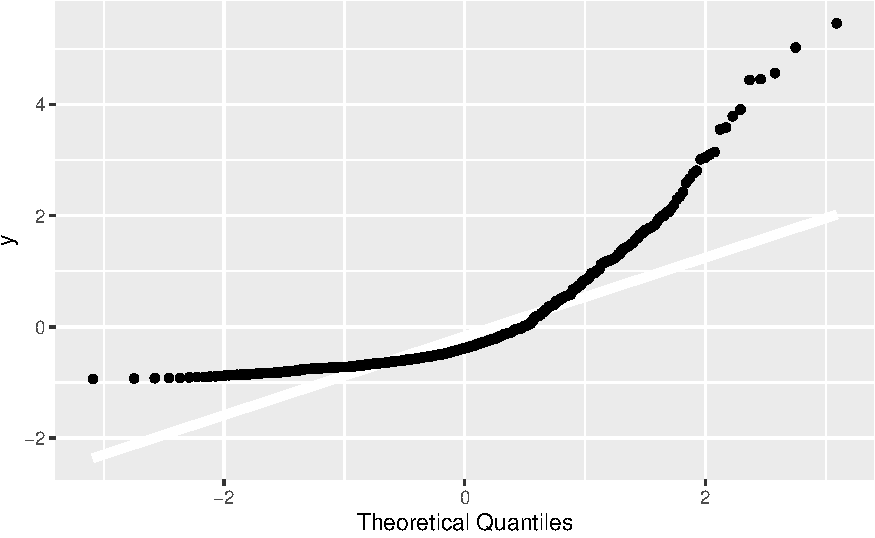
\includegraphics[width=0.7\linewidth]{regression-analysis_files/figure-latex/qqchisq-1} 

}

\caption{Q-Q plot - Positive skew}\label{fig:qqchisq}
\end{figure}

In this case, \(r_i\) is observed as heavier right tail than left. This is called \emph{positive skew} or \emph{right skew}, i.e.~its mass leans to the left.

\begin{Shaded}
\begin{Highlighting}[]
\KeywordTok{draw_qq}\NormalTok{(left, left_fit, }\DataTypeTok{col =} \KeywordTok{I}\NormalTok{(}\StringTok{"white"}\NormalTok{), }\DataTypeTok{size =} \DecValTok{2}\NormalTok{)}
\end{Highlighting}
\end{Shaded}

\begin{figure}[H]

{\centering 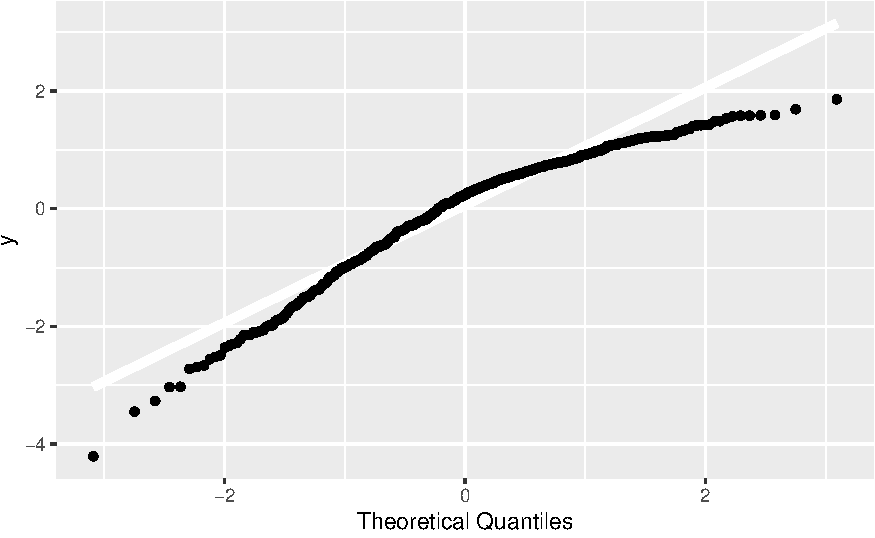
\includegraphics[width=0.7\linewidth]{regression-analysis_files/figure-latex/qqskewn-1} 

}

\caption{Q-Q plot - Negative skew}\label{fig:qqskewn}
\end{figure}

Left tail is observed heavier than right. This is called \emph{negative skew} or \emph{left skew}. Its mass leans to the right.

\hypertarget{partial-residual-plots}{%
\subsection{Partial residual plots}\label{partial-residual-plots}}

\hypertarget{outliers}{%
\section{Outliers}\label{outliers}}

An outlier is an extreme observation. Outliers occurr in two direction: \(X\) and \(Y\). There exist appropriate measures to find outliers in corresponding direction.

\hypertarget{leverage}{%
\subsection{Leverage}\label{leverage}}

Consider the design matrix and its row vectors

\[
X = \begin{bmatrix}
  \mathbf{x}_1^T \\
  \mathbf{x}_2^T \\
  \vdots \\
  \mathbf{x}_n^T
\end{bmatrix}
\]

Note that each \(\mathbf{x}_i^T = (1, x_{i1}, x_{i2}, \ldots, x_{ip})^T\) represents \(i\)-th observation.

\BeginKnitrBlock{definition}[Leverage]
\protect\hypertarget{def:hati}{}{\label{def:hati} \iffalse (Leverage) \fi{} }Let \(H\) be hat matrix, i.e.~projection onto \(Col(X)\). Then leverage is defined by its \(i\)-th diagonal element.

\[h_{ii} := \mathbf{x}_i^T (X^T X)^{-1} \mathbf{x}_i\]
\EndKnitrBlock{definition}

Let us consider the simple linear regression model, \(p = 1\). Then we have

\[
(X^T X)^{-1} = \frac{1}{\sigma^2} Var(\boldsymbol{\hat\beta}) = \begin{bmatrix}
  \bigg(\frac{1}{n} + \frac{\overline{x}^2}{S_{xx}}) & - \frac{\overline{x}}{S_{xx}} \\
  \frac{\overline{x}}{S_{xx}} & \frac{1}{S_{xx}}
\end{bmatrix}
\]

It follows that

\begin{equation*}
  \begin{split}
    h_{ii} & = \begin{bmatrix}
      1 & x_i
    \end{bmatrix} \begin{bmatrix}
    \bigg(\frac{1}{n} + \frac{\overline{x}^2}{S_{xx}}) & - \frac{\overline{x}}{S_{xx}} \\
    \frac{\overline{x}}{S_{xx}} & \frac{1}{S_{xx}}
  \end{bmatrix} \begin{bmatrix}
    1 \\
    x_i
  \end{bmatrix} \\
  & = \frac{1}{n} + \frac{(x_i - \overline{x})^2}{S_{xx}}
  \end{split}
\end{equation*}

\((x_i - \overline{x})^2\) implies that \(h_{ii}\) becomes larger as \(x_i\) is far from \(\overline{x}\). In other words, \(h_{ii}\) represents how far \(x_i\) is away from the center. Extending to \(p\), \(h_{ii}\) represents \emph{how far} \(\mathbf{x}_i\) \emph{is away from the center of observations}.

\BeginKnitrBlock{proposition}[Properties of $h_{ii}$]
\protect\hypertarget{prp:hii}{}{\label{prp:hii} \iffalse (Properties of \(h_{ii}\)) \fi{} }Leverage values \(h_{ii}\) possess several properties

\begin{enumerate}
  \item $\frac{1}{n} \le h_{ii} \le 1$
  \item $\sum\limits_{i = 1}^n h_{ii} = p + 1 \Rightarrow \overline{h} = \frac{1}{n} \sum h_{ii} = \frac{p + 1}{n}$
  \item $Var(\hat{Y_i}) = h_{ii}\sigma^2$
\end{enumerate}
\EndKnitrBlock{proposition}

\BeginKnitrBlock{conjecture}[High leverage point]
\protect\hypertarget{cnj:highlev}{}{\label{cnj:highlev} \iffalse (High leverage point) \fi{} }If \(h_{ii} > 2\overline{h} = \frac{2(p + 1)}{n}\) (twice the average value), then we regard \(i\)-th observation as \textbf{\textit{high leverage point}}.

If \(i\)-th observation is a high leverage point, we can consider that this observation is \textbf{\textit{unusual}} in \(X\)-space.
\EndKnitrBlock{conjecture}

In \texttt{R}, \(h_{ii}\) can be get in various ways. \texttt{influence()} returns \texttt{list} including \texttt{hat} which is leverage values. \texttt{broom::augment()} has a column \texttt{.hat} and this is the leverage values.

\begin{Shaded}
\begin{Highlighting}[]
\NormalTok{broom}\OperatorTok{::}\KeywordTok{augment}\NormalTok{(cem_fit) }\OperatorTok\StringTok{ }
\StringTok{  }\KeywordTok{select}\NormalTok{(.hat)}
\CommentTok{#> # A tibble: 13 x 1}
\CommentTok{#>    .hat}
\CommentTok{#>   <dbl>}
\CommentTok{#> 1 0.550}
\CommentTok{#> 2 0.333}
\CommentTok{#> 3 0.577}
\CommentTok{#> 4 0.295}
\CommentTok{#> 5 0.358}
\CommentTok{#> 6 0.124}
\CommentTok{#> # ... with 7 more rows}
\end{Highlighting}
\end{Shaded}

High leverage point is potentially dangerous for estimation of regression coefficients.

\[\hat{Y}_i = h_{i1} Y_1 + h_{i2} Y_2 + \cdots + {\color{red}{h_{ii}}} Y_i + \cdots + h_{in} Y_n\]

\(h_{ii}\) is a function of \(\mathbf{x}_i\). By construction, it measures a role of each \(\mathbf{x}_i\) in weight of observation \(Y_i\) in determining \(\hat{Y}_i\). So a small change of \(Y_i\) corresponding to a high leverage can dramatically change the estimators. However, \emph{high leverage points are not always influential points}.

\hypertarget{influence-measure}{%
\subsection{Influence measure}\label{influence-measure}}

Influence points are the points that can change the values of estimates by their existence. To see the influence of each data point, we can focus on this meaning. \emph{How much would the regression results change if the} \(i\)\emph{-th observation were deleted?}

Consdier \(D_{(-i)}\). Let \(X_{(-i)} \in (n - 1) \times (p + 1)\) be the design matrix from this data set, i.e.~design matrix without \(i\)-th observation.

\BeginKnitrBlock{lemma}
\protect\hypertarget{lem:xtranx}{}{\label{lem:xtranx} }Let \(X\) be any design matrix. Then

\[
X = \begin{bmatrix}
  \mathbf{x}_1^T \\
  \vdots \\
  \mathbf{x}_i^T \\
  \vdots \\
  \mathbf{x}_n^T
\end{bmatrix}
\]

where \(\mathbf{x}_i = (1, \mathbf{x}_{i1}, \ldots, \mathbf{x}_{ip})^T\). By construction,

\[X^T X = \sum_{i = 1}^n \mathbf{x}_i \mathbf{x}_i^T\]

Let \(Y = (Y_1, \ldots, Y_n)^T\) be any observation vector. Then

\[X^T \mathbf{Y} = \sum_{i = 1}^n \mathbf{x}_i Y_i\]
\EndKnitrBlock{lemma}

\BeginKnitrBlock{proof}
\iffalse{} {Proof. } \fi{}It is just arithmetic.

\[
X^TX = \begin{bmatrix}
  \mathbf{x}_1 & \cdots & \mathbf{x}_i & \cdots & \mathbf{x}_n
\end{bmatrix} \begin{bmatrix}
  \mathbf{x}_1^T \\
  \vdots \\
  \mathbf{x}_i^T \\
  \vdots \\
  \mathbf{x}_n^T
\end{bmatrix} = \sum_{i = 1}^n \mathbf{x}_i \mathbf{x}_i^T
\]

and

\[
X^T \mathbf{Y} = \begin{bmatrix}
  \mathbf{x}_1 & \cdots & \mathbf{x}_i & \cdots & \mathbf{x}_n
\end{bmatrix} \begin{bmatrix}
  Y_1 \\
  \vdots \\
  Y_i \\
  \vdots \\
  Y_n
\end{bmatrix} = \sum_{i = 1}^n \mathbf{x}_i Y_i
\]
\EndKnitrBlock{proof}

\BeginKnitrBlock{lemma}
\protect\hypertarget{lem:suminv}{}{\label{lem:suminv} }It can be shown that

\[(A + BCB)^{-1} = A^{-1} - A^{-1}B(C^{-1} + B^TA^{-1}B)^{-1}B^TA^{-1}\]
\EndKnitrBlock{lemma}

From Lemma \ref{lem:xtranx},

\begin{equation}
  \begin{split}
    \boldsymbol{\hat\beta}_{(-i)} & = (X_{(-i)}^T X_{(-i)})^{-1} X_{(-i)}^T \mathbf{Y}_{(-i)} \\
    & = \bigg(\sum_{j \neq i} \mathbf{x}_j \mathbf{x}_j^T \bigg)^{-1} \bigg( \sum_{j \neq i} \mathbf{x}_j Y_j \bigg) \\
    & = (X^TX - \mathbf{x}_i \mathbf{x}_i^T)^{-1} (X^T\mathbf{Y} - \mathbf{x}_i Y_i)
  \end{split}
  \label{eq:hbnoi}
\end{equation}

In Lemma \ref{lem:suminv}, take \(A = X^TX\), \(B = \mathbf{x}_i\), and \(C = -1\). It gives that

\begin{equation*}
  \begin{split}
    (X^TX - \mathbf{x}_i \mathbf{x}_i^T)^{-1} & = (X^TX)^{-1} - (X^TX)^{-1}\mathbf{x}_i (-1 + \mathbf{x}_i^T (X^TX)^{-1}\mathbf{x}_i )^{-1} \mathbf{x}_i^T (X^TX)^{-1} \\
    & = (X^TX)^{-1} + \frac{1}{1 - h_{ii}} (X^TX)^{-1} \mathbf{x}_i \mathbf{x}_i^T (X^TX)^{-1}
  \end{split}
\end{equation*}

Thus,

\begin{equation*}
  \begin{split}
    \boldsymbol{\hat\beta}_{(-i)} & = (X^TX - \mathbf{x}_i \mathbf{x}_i^T)^{-1} (X^T\mathbf{Y} - \mathbf{x}_i Y_i) \\
    & = \bigg[ (X^TX)^{-1} + \frac{1}{1 - h_{ii}} (X^TX)^{-1} \mathbf{x}_i \mathbf{x}_i^T (X^TX)^{-1} \bigg] (X^T\mathbf{Y} - \mathbf{x}_i Y_i) \\
    & = (X^TX)^{-1}X^T\mathbf{Y} - (X^TX)^{-1}\mathbf{x}_i Y_i \\
    & \qquad + \frac{1}{1 - h_{ii}} (X^TX)^{-1} \mathbf{x}_i \mathbf{x}_i^T (X^TX)^{-1} X^T \mathbf{Y} -  \frac{1}{1 - h_{ii}} (X^TX)^{-1} \mathbf{x}_i \mathbf{x}_i^T (X^TX)^{-1} \mathbf{x}_i Y_i \\
    & = \boldsymbol{\hat\beta}- (X^TX)^{-1}\mathbf{x}_i Y_i + \frac{1}{1 - h_{ii}} (X^TX)^{-1} \mathbf{x}_i \mathbf{x}_i^T \boldsymbol{\hat\beta}- \frac{h_{ii}}{1 - h_{ii}} (X^TX)^{-1} \mathbf{x}_i Y_i \\
    & = \boldsymbol{\hat\beta}- \bigg[ 1 + \frac{h_{ii}}{1 - h_{ii}} \bigg] (X^TX)^{-1} \mathbf{x}_i Y_i + \frac{1}{1 - h_{ii}} (X^TX)^{-1} \mathbf{x}_i \hat{Y}_i \quad \because \mathbf{x}_i^T \boldsymbol{\hat\beta}= \hat{Y}_i \\
    & = \boldsymbol{\hat\beta}- \frac{1}{1 - h_{ii}} (X^TX)^{-1} \mathbf{x}_i ( Y_i - \hat{Y}_i) \quad \because 1 + \frac{h_{ii}}{1 - h_{ii}} = \frac{1}{1 - h_{ii}} \\
    & = \boldsymbol{\hat\beta}- \frac{1}{1 - h_{ii}} (X^TX)^{-1} \mathbf{x}_i e_i
  \end{split}
\end{equation*}

\BeginKnitrBlock{theorem}
\protect\hypertarget{thm:hbnoithm}{}{\label{thm:hbnoithm} }Regression coefficient without \(i\)-th observation can come from the original desing matrix. Also, it is affected by \(i\)-th residual.

\[\boldsymbol{\hat\beta}_{(-i)} = \boldsymbol{\hat\beta}- \frac{1}{1 - h_{ii}} (X^TX)^{-1} \mathbf{x}_i e_i\]
\EndKnitrBlock{theorem}

\hypertarget{press-residual}{%
\subsection{PRESS residual}\label{press-residual}}

See Theorem \ref{thm:hbnoithm}. Previous residuals might be able to detect outliers. However, other kind of residuals can be considered here.

\BeginKnitrBlock{definition}[PRESS residuals]
\protect\hypertarget{def:prsresid}{}{\label{def:prsresid} \iffalse (PRESS residuals) \fi{} }\(PRESS\) residuals are defined by

\[e_{i, -i} = Y_i - \hat{Y}_{i, -i}\]

where \(\hat{Y}_{i, -i} = \mathbf{x}_i^T \boldsymbol{\hat\beta}_{(-i)}\) is the fitted value of the \(i\)-th response without \(i\)-th observation.
\EndKnitrBlock{definition}

Note that

\[\hat{Y}_{i, -i} = \mathbf{x}_i^T \boldsymbol{\hat\beta}_{(-i)}\]

From Theorem \ref{thm:hbnoithm}, we can get a useful identity about PRESS residual.

\BeginKnitrBlock{theorem}
\protect\hypertarget{thm:prsraw}{}{\label{thm:prsraw} }PRESS residuals are related to Raw residuals \(e_i\) and leverage values \(h_{ii}\).

\[e_{i, -i} = \frac{e_i}{1 - h_{ii}}\]
\EndKnitrBlock{theorem}

\BeginKnitrBlock{proof}
\iffalse{} {Proof. } \fi{}Theorem \ref{thm:hbnoithm} implies that

\begin{equation*}
  \begin{split}
    e_{i, -i} & = Y_i - \hat{Y}_{i, -i} \\
    & = Y_i - \mathbf{x}_i^T \boldsymbol{\hat\beta}_{(-i)} \\
    & = Y_i - \mathbf{x}_i^T \bigg[  \boldsymbol{\hat\beta}- \frac{1}{1 - h_{ii}} (X^TX)^{-1} \mathbf{x}_i e_i \bigg] \\
    & = Y_i - \mathbf{x}_i^T \boldsymbol{\hat\beta}+ \frac{h_{ii}}{1 - h_{ii}}e_i \\
    & = \frac{e_i}{1 - h_{ii}} \quad \because Y_i - \mathbf{x}_i^T \boldsymbol{\hat\beta}= e_i
  \end{split}
\end{equation*}
\EndKnitrBlock{proof}

Althogh the definition of PRESS requires refitting different models, this Thoerem \ref{thm:prsraw} let us easily compute \(e_{i, -i}\) without refitting data.

\BeginKnitrBlock{remark}[Standardized PRESS residual]
\iffalse{} {Remark (Standardized PRESS residual). } \fi{}We standardize PRESS residuals \(e_{i, -i}\) by

\[\frac{e_{i, -i}}{\sqrt{Var(e_{i, -i})}} = \frac{e_i / 1 - h_{ii}}{\sqrt{\sigma^2 / (1 - h_{ii})}} = \frac{e_i}{\sigma \sqrt{1 - h_{ii}}}\]

It is same as \textit{standardized residuals} if replacing \(\sigma^2\) with \(\hat\sigma^2\).
\EndKnitrBlock{remark}

\hypertarget{dffits}{%
\subsection{DFFITS}\label{dffits}}

\BeginKnitrBlock{definition}[DFFITS]
\protect\hypertarget{def:dff}{}{\label{def:dff} \iffalse (DFFITS) \fi{} }\[(DFFITS)_i := \frac{\hat{Y}_i - \hat{Y}_{i, -i}}{\hat\sigma_{(-i)} \sqrt{h_{ii}}}\]

where \(\hat{Y}_i = \mathbf{x}_i^T \boldsymbol{\hat\beta}\) and \(\hat{Y}_{i, -i} = \mathbf{x}_i^T \boldsymbol{\hat\beta}_{(-i)}\)
\EndKnitrBlock{definition}

\BeginKnitrBlock{corollary}
\protect\hypertarget{cor:dffrepresent}{}{\label{cor:dffrepresent} }\[(DFFITS)_i = \frac{e_i}{\hat\sigma_{(-i)\sqrt{h_{ii}}}} \times \sqrt{\frac{h_{ii}}{1 - h_{ii}}} = \text{studentized residual} \times \text{leverage measure}\]
\EndKnitrBlock{corollary}

\BeginKnitrBlock{proof}
\iffalse{} {Proof. } \fi{}\begin{equation*}
  \begin{split}
    \hat{Y}_i - \hat{Y}_{i, -i} & = (Y_i - \hat{Y}_i) - (Y_i - \hat{Y}_{i, -i}) \\
    & = e_{i, -i} - e_i \\
    & = \frac{h_{ii}}{1 - h_{ii}} e_i
  \end{split}
\end{equation*}
\EndKnitrBlock{proof}

The second part represents leverage. As leverage values become large, i.e.~\(h_{ii} \rightarrow 1\) (Proposition \ref{prp:hii}), this becomes \(\infty\). This form of function expressed by \(h_{ii}\) is called \emph{potential function}

\begin{figure}[H]

{\centering 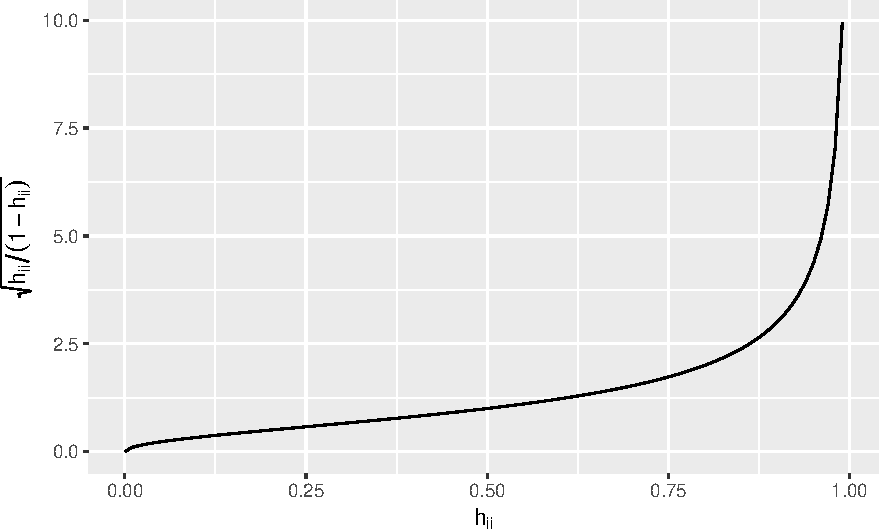
\includegraphics[width=0.7\linewidth]{regression-analysis_files/figure-latex/levmeasure-1} 

}

\caption{Shape of potential function}\label{fig:levmeasure}
\end{figure}

\BeginKnitrBlock{conjecture}[Rule of thumb]
\protect\hypertarget{cnj:dffthumb}{}{\label{cnj:dffthumb} \iffalse (Rule of thumb) \fi{} }If \(\lvert (DFFITS)_i \rvert > 2 \sqrt{\frac{p + 1}{n - p - 1}}\), then \(i\)-th observation is considered to be influential.
\EndKnitrBlock{conjecture}

There is \texttt{dffits()} so that we can easilty get only \((DFFITS)_i\) for every \(i\)

\begin{Shaded}
\begin{Highlighting}[]
\KeywordTok{tibble}\NormalTok{(}\DataTypeTok{DFFITS =} \KeywordTok{dffits}\NormalTok{(cem_fit)) }\OperatorTok\StringTok{ }
\StringTok{  }\KeywordTok{mutate}\NormalTok{(}\DataTypeTok{i =} \DecValTok{1}\OperatorTok{:}\KeywordTok{n}\NormalTok{()) }\OperatorTok\StringTok{ }
\StringTok{  }\KeywordTok{ggplot}\NormalTok{(}\KeywordTok{aes}\NormalTok{(}\DataTypeTok{x =}\NormalTok{ i, }\DataTypeTok{y =}\NormalTok{ DFFITS)) }\OperatorTok{+}
\StringTok{  }\KeywordTok{geom_ref_line}\NormalTok{(}\DataTypeTok{h =} \DecValTok{2} \OperatorTok{*}\StringTok{ }\KeywordTok{sqrt}\NormalTok{( (}\DecValTok{4} \OperatorTok{+}\StringTok{ }\DecValTok{1}\NormalTok{) }\OperatorTok{/}\StringTok{ }\NormalTok{(}\KeywordTok{nrow}\NormalTok{(cem) }\OperatorTok{-}\StringTok{ }\DecValTok{4} \OperatorTok{-}\StringTok{ }\DecValTok{1}\NormalTok{) )) }\OperatorTok{+}
\StringTok{  }\KeywordTok{geom_point}\NormalTok{() }\OperatorTok{+}
\StringTok{  }\KeywordTok{geom_linerange}\NormalTok{(}\KeywordTok{aes}\NormalTok{(}\DataTypeTok{ymin =}\NormalTok{ DFFITS, }\DataTypeTok{ymax =} \DecValTok{0}\NormalTok{), }\DataTypeTok{col =} \KeywordTok{gg_hcl}\NormalTok{(}\DecValTok{1}\NormalTok{), }\DataTypeTok{linetype =} \StringTok{"dotted"}\NormalTok{)}
\end{Highlighting}
\end{Shaded}

\begin{figure}[H]

{\centering 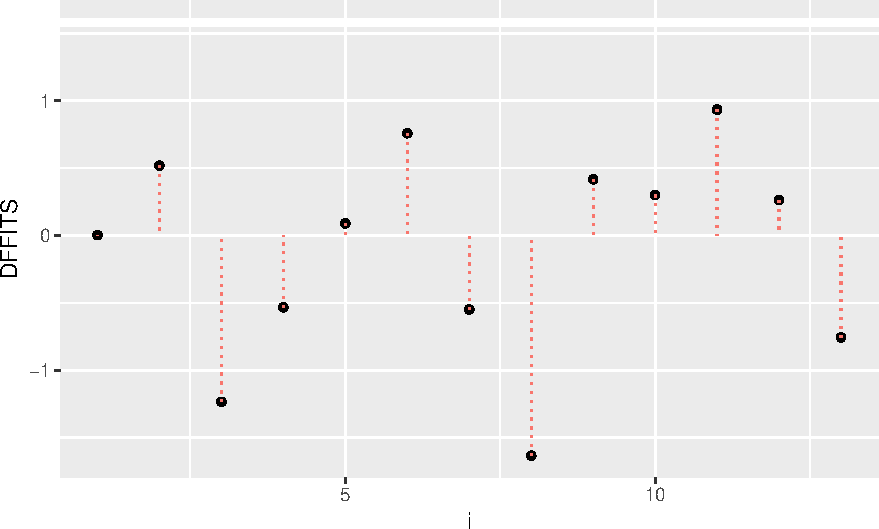
\includegraphics[width=0.7\linewidth]{regression-analysis_files/figure-latex/dffdat-1} 

}

\caption{DFFITS for fitted cement dataset}\label{fig:dffdat}
\end{figure}

\hypertarget{cooks-distance}{%
\subsection{Cook's Distance}\label{cooks-distance}}

\BeginKnitrBlock{definition}[Cook\'s distance]
\protect\hypertarget{def:cook}{}{\label{def:cook} \iffalse (Cook's distance) \fi{} }\[C_i := \frac{\sum\limits_{j = 1}^n (\hat{Y}_j - \hat{Y}_{j, -i})^2}{\hat\sigma (p + 1)}\]

where \(\hat{Y}_{j, -i} = \mathbf{x}_j^T \boldsymbol{\hat\beta}_{(-i)}\).
\EndKnitrBlock{definition}

Cook's distnace is related to the distance between \(\mathbf{\hat{Y}}\) and \(\mathbf{\hat{Y}}_{(-i)}\).

\BeginKnitrBlock{corollary}
\protect\hypertarget{cor:cookrepresent}{}{\label{cor:cookrepresent} }Cooks's distance is related to the distance between \(\boldsymbol{\hat\beta}\) and \(\boldsymbol{\hat\beta}_{(-i)}\).

\[C_i = \frac{(\boldsymbol{\hat\beta}- \boldsymbol{\hat\beta}_{(-i)})^T X^T X (\boldsymbol{\hat\beta}- \boldsymbol{\hat\beta}_{(-i)})}{\hat\sigma (p + 1)}\]
\EndKnitrBlock{corollary}

\BeginKnitrBlock{proof}
\iffalse{} {Proof. } \fi{}It is just arithmetic if plug-in \(\hat{Y}_{j} = \mathbf{x}_j^T \boldsymbol{\hat\beta}\) \(\hat{Y}_{j, -i} = \mathbf{x}_j^T \boldsymbol{\hat\beta}_{(-i)}\).

\begin{equation*}
  \begin{split}
    C_i & = \frac{(\mathbf{Y} - \mathbf{Y}_{-i})^T(\mathbf{Y} - \mathbf{Y}_{-i})}{\hat\sigma^2 (p + 1)} \\
    & = \frac{(X\boldsymbol{\hat\beta}- X\boldsymbol{\hat\beta}_{(-i)})^T(X\boldsymbol{\hat\beta}- X\boldsymbol{\hat\beta}_{(-i)})}{\hat\sigma^2 (p + 1)} \\
    & = \frac{(\boldsymbol{\hat\beta}- \boldsymbol{\hat\beta}_{(-i)})^T X^TX (\boldsymbol{\hat\beta}- \boldsymbol{\hat\beta}_{(-i)})}{\hat\sigma^2 (p + 1)}
  \end{split}
\end{equation*}
\EndKnitrBlock{proof}

\BeginKnitrBlock{remark}
\iffalse{} {Remark. } \fi{}\(C_i\) can be represented by internally studentized residual and potential function

\[C_i = \bigg( \frac{e_i}{\hat\sigma \sqrt{1 - h_{ii}}} \bigg)^2 \times \frac{1}{p + 1} \times \frac{h_{ii}}{1 - h_{ii}}\]
\EndKnitrBlock{remark}

\BeginKnitrBlock{proof}
\iffalse{} {Proof. } \fi{}From Theorem \ref{thm:hbnoithm} (\(\boldsymbol{\hat\beta}_{(-i)} = \boldsymbol{\hat\beta}- \frac{1}{1 - h_{ii}} (X^TX)^{-1} \mathbf{x}_i e_i\)) and Corollary \ref{cor:cookrepresent},

\begin{equation*}
  \begin{split}
    C_i & = \frac{(\boldsymbol{\hat\beta}- \boldsymbol{\hat\beta}_{(-i)})^T X^TX (\boldsymbol{\hat\beta}- \boldsymbol{\hat\beta}_{(-i)})}{\hat\sigma^2 (p + 1)} \\
    & = \frac{\Big[ \frac{1}{1 - h_{ii}} (X^TX)^{-1} \mathbf{x}_i e_i \Big]^T X^TX \Big[ \frac{1}{1 - h_{ii}} (X^TX)^{-1} \mathbf{x}_i e_i \Big]}{\hat\sigma^2 (p + 1)} \\
    & = \frac{\frac{e_i^2}{(1 - h_{ii})^2} \mathbf{x}_i (X^TX)^{-1} \mathbf{x}_i}{\hat\sigma^2 (p + 1)} \\
    & = \bigg( \frac{e_i}{\hat\sigma \sqrt{1 - h_{ii}}} \bigg)^2 \times \frac{1}{p + 1} \times \frac{h_{ii}}{1 - h_{ii}} \quad \because \mathbf{x}_i (X^TX)^{-1} \mathbf{x}_i = h_{ii} \\
    & = (\text{internally studentized residual})^2 \times \frac{1}{p + 1} \times \text{leverage measure}
  \end{split}
\end{equation*}
\EndKnitrBlock{proof}

\BeginKnitrBlock{conjecture}
\protect\hypertarget{cnj:cookthumb}{}{\label{cnj:cookthumb} }In practice, if \(C_i > 1\), \(i\)-th observation is considered to be influential.
\EndKnitrBlock{conjecture}

Corollary \ref{cor:cookrepresent} is form of \(F\)-statistic. More specifically, \(F(p, n - p)\). \(1\) is actually come from \(F_{0.5} (p, n - p)\). If the case is out of 50th percentile of \(F\)-distribution, then we will say that it is influential point.

In \texttt{R}, \texttt{cooks.distance()} gives \(C_i\) alone.

\begin{Shaded}
\begin{Highlighting}[]
\KeywordTok{tibble}\NormalTok{(}\DataTypeTok{cook =} \KeywordTok{cooks.distance}\NormalTok{(cem_fit)) }\OperatorTok\StringTok{ }
\StringTok{  }\KeywordTok{mutate}\NormalTok{(}\DataTypeTok{i =} \DecValTok{1}\OperatorTok{:}\KeywordTok{n}\NormalTok{()) }\OperatorTok\StringTok{ }
\StringTok{  }\KeywordTok{ggplot}\NormalTok{(}\KeywordTok{aes}\NormalTok{(}\DataTypeTok{x =}\NormalTok{ i, }\DataTypeTok{y =}\NormalTok{ cook)) }\OperatorTok{+}
\StringTok{  }\KeywordTok{geom_ref_line}\NormalTok{(}\DataTypeTok{h =} \DecValTok{1}\NormalTok{) }\OperatorTok{+}
\StringTok{  }\KeywordTok{geom_point}\NormalTok{() }\OperatorTok{+}
\StringTok{  }\KeywordTok{geom_linerange}\NormalTok{(}\KeywordTok{aes}\NormalTok{(}\DataTypeTok{ymin =}\NormalTok{ cook, }\DataTypeTok{ymax =} \DecValTok{0}\NormalTok{), }\DataTypeTok{col =} \KeywordTok{gg_hcl}\NormalTok{(}\DecValTok{1}\NormalTok{), }\DataTypeTok{linetype =} \StringTok{"dotted"}\NormalTok{)}
\end{Highlighting}
\end{Shaded}

\begin{figure}[H]

{\centering 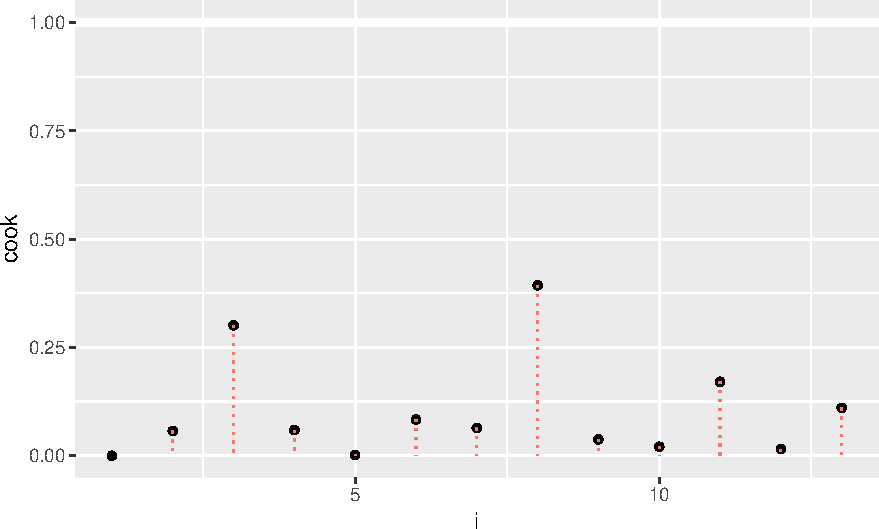
\includegraphics[width=0.7\linewidth]{regression-analysis_files/figure-latex/cidat-1} 

}

\caption{Cook\'s Distance for fitted cement dataset}\label{fig:cidat}
\end{figure}

In fact, we can get every influential statistic at once. \texttt{influence()} gives as \texttt{list} object.

\begin{Shaded}
\begin{Highlighting}[]
\KeywordTok{influence}\NormalTok{(cem_fit)}
\CommentTok{#> $hat}
\CommentTok{#>     1     2     3     4     5     6     7     8     9    10    11    12 }
\CommentTok{#> 0.550 0.333 0.577 0.295 0.358 0.124 0.367 0.409 0.294 0.700 0.426 0.263 }
\CommentTok{#>    13 }
\CommentTok{#> 0.304 }
\CommentTok{#> }
\CommentTok{#> $coefficients}
\CommentTok{#>    (Intercept)        x1        x2        x3        x4}
\CommentTok{#> 1      -0.0797  0.000615  0.000865  0.000563  0.000923}
\CommentTok{#> 2      14.3977 -0.188059 -0.144479 -0.166288 -0.130195}
\CommentTok{#> 3     -76.1808  0.763715  0.777935  0.811840  0.772107}
\CommentTok{#> 4     -16.9320  0.135355  0.183354  0.170637  0.163203}
\CommentTok{#> 5      -1.4097  0.002222  0.018383  0.002002  0.017145}
\CommentTok{#> 6      11.3466 -0.078436 -0.114107 -0.113965 -0.119354}
\CommentTok{#> 7       3.8884 -0.003697 -0.053510 -0.042756 -0.031897}
\CommentTok{#> 8      25.1599 -0.328637 -0.223616 -0.416775 -0.248256}
\CommentTok{#> 9      18.0763 -0.202827 -0.182419 -0.176212 -0.185153}
\CommentTok{#> 10     -3.9568  0.092798  0.031933  0.063502  0.035052}
\CommentTok{#> 11    -22.6795  0.278931  0.213431  0.345600  0.217330}
\CommentTok{#> 12    -10.0419  0.106271  0.107888  0.101899  0.098533}
\CommentTok{#> 13     24.5346 -0.219201 -0.274452 -0.214449 -0.247089}
\CommentTok{#> }
\CommentTok{#> $sigma}
\CommentTok{#>    1    2    3    4    5    6    7    8    9   10   11   12   13 }
\CommentTok{#> 2.61 2.52 2.43 2.50 2.61 2.08 2.52 2.10 2.54 2.61 2.42 2.58 2.40 }
\CommentTok{#> }
\CommentTok{#> $wt.res}
\CommentTok{#>        1        2        3        4        5        6        7        8 }
\CommentTok{#>  0.00476  1.51120 -1.67094 -1.72710  0.25076  3.92544 -1.44867 -3.17499 }
\CommentTok{#>        9       10       11       12       13 }
\CommentTok{#>  1.37835  0.28155  1.99098  0.97299 -2.29433}
\end{Highlighting}
\end{Shaded}

On the other hand, \texttt{influence.measures()} gives \texttt{matrix}. Its class is \texttt{infl} and we can extract \texttt{matrix} by \texttt{\$infmat}.

\begin{Shaded}
\begin{Highlighting}[]
\KeywordTok{influence.measures}\NormalTok{(cem_fit)}
\CommentTok{#> Influence measures of}
\CommentTok{#>   lm(formula = y ~ ., data = cem) :}
\CommentTok{#> }
\CommentTok{#>      dfb.1_    dfb.x1   dfb.x2    dfb.x3   dfb.x4   dffit cov.r   cook.d}
\CommentTok{#> 1  -0.00106  0.000773  0.00112  0.000698  0.00122  0.0030 4.335 2.06e-06}
\CommentTok{#> 2   0.19947 -0.245131 -0.19378 -0.213899 -0.17826  0.5193 2.017 5.72e-02}
\CommentTok{#> 3  -1.09529  1.033072  1.08281  1.083708  1.09704 -1.2356 2.195 3.01e-01}
\CommentTok{#> 4  -0.23674  0.178058  0.24819  0.221515  0.22551 -0.5333 1.741 5.93e-02}
\CommentTok{#> 5  -0.01884  0.002793  0.02378  0.002484  0.02264  0.0894 3.004 1.82e-03}
\CommentTok{#> 6   0.19047 -0.123878 -0.18544 -0.177619 -0.19800  0.7594 0.225 8.34e-02}
\CommentTok{#> 7   0.05380 -0.004812 -0.07168 -0.054930 -0.04362 -0.5497 2.151 6.43e-02}
\CommentTok{#> 8   0.41856 -0.514380 -0.36015 -0.643741 -0.40814 -1.6352 0.365 3.94e-01}
\CommentTok{#> 9   0.24840 -0.262227 -0.24268 -0.224818 -0.25144  0.4171 2.068 3.75e-02}
\CommentTok{#> 10 -0.05297  0.116875  0.04138  0.078926  0.04637  0.3016 6.330 2.07e-02}
\CommentTok{#> 11 -0.32727  0.378689  0.29816  0.463023  0.30992  0.9345 1.558 1.71e-01}
\CommentTok{#> 12 -0.13589  0.135302  0.14134  0.128027  0.13177  0.2625 2.309 1.53e-02}
\CommentTok{#> 13  0.35692 -0.300024 -0.38654 -0.289655 -0.35523 -0.7568 1.185 1.10e-01}
\CommentTok{#>      hat inf}
\CommentTok{#> 1  0.550   *}
\CommentTok{#> 2  0.333    }
\CommentTok{#> 3  0.577   *}
\CommentTok{#> 4  0.295    }
\CommentTok{#> 5  0.358   *}
\CommentTok{#> 6  0.124    }
\CommentTok{#> 7  0.367    }
\CommentTok{#> 8  0.409    }
\CommentTok{#> 9  0.294    }
\CommentTok{#> 10 0.700   *}
\CommentTok{#> 11 0.426    }
\CommentTok{#> 12 0.263    }
\CommentTok{#> 13 0.304}
\end{Highlighting}
\end{Shaded}

In \texttt{broom} package, \texttt{broom::augment()} includes influene measures. To use \texttt{tibble}, we can use this function.

\begin{Shaded}
\begin{Highlighting}[]
\NormalTok{broom}\OperatorTok{::}\KeywordTok{augment}\NormalTok{(cem_fit)}
\CommentTok{#> # A tibble: 13 x 12}
\CommentTok{#>       y    x1    x2    x3    x4 .fitted .se.fit   .resid  .hat .sigma}
\CommentTok{#>   <dbl> <dbl> <dbl> <dbl> <dbl>   <dbl>   <dbl>    <dbl> <dbl>  <dbl>}
\CommentTok{#> 1  78.5     7    26     6    60    78.5   1.81   0.00476 0.550   2.61}
\CommentTok{#> 2  74.3     1    29    15    52    72.8   1.41   1.51    0.333   2.52}
\CommentTok{#> 3 104.     11    56     8    20   106.    1.86  -1.67    0.577   2.43}
\CommentTok{#> 4  87.6    11    31     8    47    89.3   1.33  -1.73    0.295   2.50}
\CommentTok{#> 5  95.9     7    52     6    33    95.6   1.46   0.251   0.358   2.61}
\CommentTok{#> 6 109.     11    55     9    22   105.    0.862  3.93    0.124   2.08}
\CommentTok{#> # ... with 7 more rows, and 2 more variables: .cooksd <dbl>,}
\CommentTok{#> #   .std.resid <dbl>}
\end{Highlighting}
\end{Shaded}

\hypertarget{remedial-measures}{%
\section{Remedial Measures}\label{remedial-measures}}

In many times, given data set violates our assumptions. We have seen some of those scenarios. In that case, typical procedure will not be welcomed.

\hypertarget{transformations}{%
\subsection{Transformations}\label{transformations}}

As quick remedies for violations, transformations of variables can be conducted.

First, See Figure \ref{fig:heteropt}. When \textbf{variance becomes larger} as \(\hat{Y}_i\) increases, transform \(Y_i\) into

\[\ln Y_i \quad \text{or} \quad \sqrt{Y_i}\]

i.e.~the model becomes

\[
\begin{cases}
\ln Y_i = \beta_0 + \beta_1 x_{i1} + \cdots \beta_p x_{ip} + \epsilon_i \\
\sqrt{Y_i} = \beta_0 + \beta_1 x_{i1} + \cdots \beta_p x_{ip} + \epsilon_i
\end{cases}
\]

Since \(\ln(.)\) and \(\sqrt{.}\) is increasing with decreasing derivative, it might be able to suppress increasing variance which is depending on \(\hat{Y}_i\).

\begin{Shaded}
\begin{Highlighting}[]
\NormalTok{hetero_scale <-}\StringTok{ }
\StringTok{  }\NormalTok{hetero }\OperatorTok\StringTok{ }
\StringTok{  }\KeywordTok{mutate}\NormalTok{(}
    \DataTypeTok{logy =} \KeywordTok{log}\NormalTok{(y }\OperatorTok{-}\StringTok{ }\KeywordTok{min}\NormalTok{(y) }\OperatorTok{+}\StringTok{ }\FloatTok{.1}\NormalTok{),}
    \DataTypeTok{sqy =} \KeywordTok{sqrt}\NormalTok{(y }\OperatorTok{-}\StringTok{ }\KeywordTok{min}\NormalTok{(y) }\OperatorTok{+}\StringTok{ }\FloatTok{.1}\NormalTok{)}
\NormalTok{  )}
\CommentTok{#--------------}
\NormalTok{hetero_log <-}\StringTok{ }\KeywordTok{lm}\NormalTok{(logy }\OperatorTok{~}\StringTok{ }\NormalTok{x, }\DataTypeTok{data =}\NormalTok{ hetero_scale)}
\NormalTok{hetero_sqrt <-}\StringTok{ }\KeywordTok{lm}\NormalTok{(sqy }\OperatorTok{~}\StringTok{ }\NormalTok{x, }\DataTypeTok{data =}\NormalTok{ hetero_scale)}
\end{Highlighting}
\end{Shaded}

\begin{Shaded}
\begin{Highlighting}[]
\KeywordTok{residplot}\NormalTok{(hetero_scale, hetero_log)}
\end{Highlighting}
\end{Shaded}

\begin{figure}[H]

{\centering 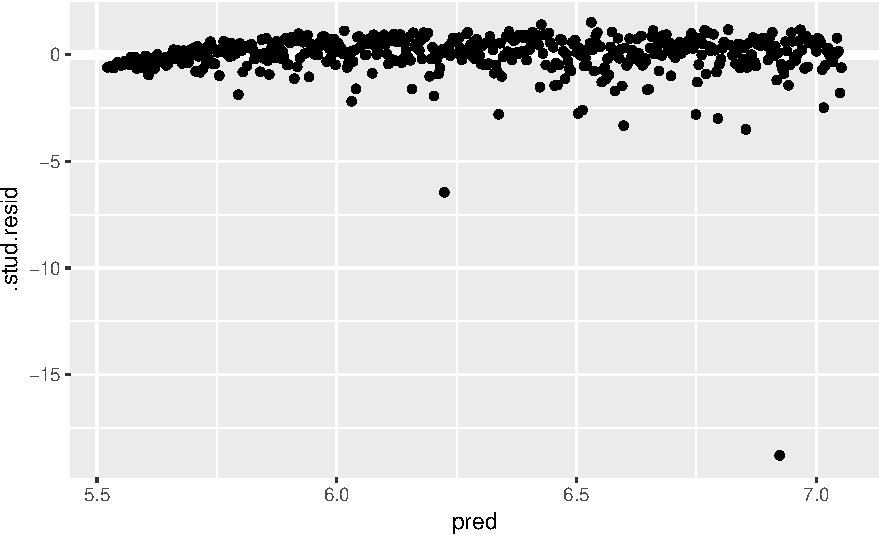
\includegraphics[width=0.7\linewidth]{regression-analysis_files/figure-latex/heterolog-1} 

}

\caption{Log transformation against increasing variance}\label{fig:heterolog}
\end{figure}

\begin{Shaded}
\begin{Highlighting}[]
\KeywordTok{residplot}\NormalTok{(hetero_scale, hetero_sqrt)}
\end{Highlighting}
\end{Shaded}

\begin{figure}[H]

{\centering \includegraphics[width=0.7\linewidth]{regression-analysis_files/figure-latex/heterosqrt-1} 

}

\caption{Square root transformation against increasing variance}\label{fig:heterosqrt}
\end{figure}

See Figures \ref{fig:heterolog} and \ref{fig:heterosqrt}. In this example, log-transformation was more affective. This might be because log function is smaller than square root function in large values.

Second, see Figure \ref{fig:nonlinpt}. Sometimes we observe a \textbf{certain pattern} in residual plot. Here, non-linear - cubic. Then transform \(x_i\) into corresponding non-linear function of \(x_i\).

\begin{Shaded}
\begin{Highlighting}[]
\NormalTok{cubic_poly <-}\StringTok{ }\KeywordTok{lm}\NormalTok{(y }\OperatorTok{~}\StringTok{ }\KeywordTok{poly}\NormalTok{(x, }\DecValTok{3}\NormalTok{), }\DataTypeTok{data =}\NormalTok{ cubic) }\CommentTok{# cubic polynomial}
\KeywordTok{residplot}\NormalTok{(cubic, cubic_poly)}
\end{Highlighting}
\end{Shaded}

\begin{figure}[H]

{\centering \includegraphics[width=0.7\linewidth]{regression-analysis_files/figure-latex/cubicregress-1} 

}

\caption{Cubic transformation against cubic pattern}\label{fig:cubicregress}
\end{figure}

Third, consider the case when Q-Q plot shows \textbf{non-normality}. Of course it depends on a situation, but

\[\ln Y_i\]

helpful sometimes.

\hypertarget{variance-stabilizing-transformation}{%
\subsection{Variance stabilizing transformation}\label{variance-stabilizing-transformation}}

Suppose that the variance is \textbf{not constant} and it is the \textbf{function of mean}.

\[Y_i = \beta_0 + \beta_1 x_{i1} + \cdots + \beta_p x_{ip} + \epsilon_{i}, \quad \epsilon_i \sim N(0, f^2(\mu_i))\]

where \(\mu_i = E(Y_i)\) and \(f\) is a smooth function for \emph{standard deviation}. Before looking at how to deal with this heteroskedasticity, review a theorem from mathematical statistics.

\BeginKnitrBlock{theorem}[Delta Method of moments]
\protect\hypertarget{thm:delthm}{}{\label{thm:delthm} \iffalse (Delta Method of moments) \fi{} }Let \(h(Y_i)\) be any change of variable.

\[E[h(Y_i)] \approx h(Y_i)\]

and

\[Var[h(Y_i)] \approx \Big(h^{\prime}(\mu_i)\Big)^2 Var(Y_i)\]
\EndKnitrBlock{theorem}

\BeginKnitrBlock{proof}
\iffalse{} {Proof. } \fi{}Taylor formula implies that

\[h(Y_i) \approx h(\mu_i) + h^{\prime}(\mu_i)(Y_i - \mu_i)\]

Then by taking mean and variance,

\[Eh(Y_i) \approx h(Y_i)\]

\[Var h(Y_i) \approx \Big( h^{\prime}(\mu_i) \Big)^2 Var(Y_i)\]
\EndKnitrBlock{proof}

We try to find some \emph{variance stabilizing transformation} \(h(Y_i)\) such that

\[Var[h(Y_i)] = \sigma^2\]

From Theorem \ref{thm:delthm},

\begin{equation}
  \sigma^2 \approx \Big( h^{\prime}(\mu_i) \Big)^2 f^2 (\mu_i)
  \label{eq:vstsig}
\end{equation}

It follows that

\begin{equation*}
  \begin{split}
    & h^{\prime}(\mu_i) \approx \frac{\sigma}{f(\mu_i)} \\
    & \Rightarrow h^{\prime}(\mu_i) \propto \frac{1}{f(\mu_i)} \\
    & \Rightarrow h(\mu_i) \propto \int \frac{1}{f(\mu_i)} d\mu_i
  \end{split}
\end{equation*}

\BeginKnitrBlock{theorem}[Variance stabilizing transformation]
\protect\hypertarget{thm:vst}{}{\label{thm:vst} \iffalse (Variance stabilizing transformation) \fi{} }\(h\) can be calculated by

\[h(\mu_i) \propto \int \frac{1}{f(\mu_i)} d\mu_i\]
\EndKnitrBlock{theorem}

Theorem \ref{thm:vst} shows how we can stabilize variance using the direct pattern of variance.

\BeginKnitrBlock{example}[Poisson error term]
\protect\hypertarget{exm:poiserr}{}{\label{exm:poiserr} \iffalse (Poisson error term) \fi{} }\[Y_i \mid \mathbf{x}_i \stackrel{indep}{\sim}Poisson(\lambda(\mathbf{x}_i))\]
\EndKnitrBlock{example}

\begin{Shaded}
\begin{Highlighting}[]
\KeywordTok{residplot}\NormalTok{(vst_pois, pois_fit)}
\end{Highlighting}
\end{Shaded}

\begin{figure}[H]

{\centering \includegraphics[width=0.7\linewidth]{regression-analysis_files/figure-latex/vstpois1-1} 

}

\caption{Residual plot after fitting Poisson error model}\label{fig:vstpois1}
\end{figure}

\BeginKnitrBlock{solution}
\iffalse{} {Solution. } \fi{}Poisson error term results in non-constant variance. It is natural because the variance is the same as mean

\[Var(Y_i \mid \mathbf{x}_i) = E(Y_i \mid \mathbf{x}_i) = \lambda(\mathbf{x}_i)\]

Let \(\lambda_i \equiv \lambda(\mathbf{x}_i)\). Applying VST,

\[h(\lambda_i) \propto \int \frac{1}{\sqrt{\lambda_i}} d\lambda_i \propto 2 \sqrt{\lambda_i}\]

Hence, we set VST by

\[h(Y_i) = \sqrt{Y_i}\]
\EndKnitrBlock{solution}

\begin{Shaded}
\begin{Highlighting}[]
\NormalTok{vst_pois <-}\StringTok{ }
\StringTok{  }\NormalTok{vst_pois }\OperatorTok\StringTok{ }
\StringTok{  }\KeywordTok{mutate}\NormalTok{(}\DataTypeTok{ysq =} \KeywordTok{sqrt}\NormalTok{(y))}
\NormalTok{vstpois_fit <-}\StringTok{ }\KeywordTok{lm}\NormalTok{(ysq }\OperatorTok{~}\StringTok{ }\NormalTok{x, }\DataTypeTok{data =}\NormalTok{ vst_pois)}
\CommentTok{#--------------}
\KeywordTok{residplot}\NormalTok{(vst_pois, vstpois_fit)}
\end{Highlighting}
\end{Shaded}

\begin{figure}[H]

{\centering \includegraphics[width=0.7\linewidth]{regression-analysis_files/figure-latex/vstpois2-1} 

}

\caption{Poisson error term model residuals after VST}\label{fig:vstpois2}
\end{figure}

In fact, a \emph{better way is to fit Poisson regression model, as a special case of generalized linera models}. This can explain Poisson random error with random component.

In general, we do not know \(f\). In this case, we just

\begin{enumerate}
\def\labelenumi{\arabic{enumi}.}
\tightlist
\item
  trial and error
\item
  previous results
\item
  If replications (multiple observations of \(Y_i\) at same \(\mathbf{x}_i\) values) exist

  \begin{enumerate}
  \def\labelenumii{\arabic{enumii}.}
  \tightlist
  \item
    compute sd \(S_i\) and average \(\overline{Y}_i\)
  \item
    simple linear regression \(S_i = \alpha + \lambda \overline{Y}_i\)
  \item
    \(f(\mu_i) = \hat\alpha \mu_i^{\hat\lambda}\)
  \end{enumerate}
\item
  If no replication, group
\end{enumerate}

\hypertarget{box-cox-transformation}{%
\subsection{Box-Cox Transformation}\label{box-cox-transformation}}

\emph{Box-Cox transformation} is usually considered when Normality assumption is violated.

\[
Y^{\prime} = \begin{cases}
  \frac{Y^{\lambda} - 1}{\lambda} & \text{if}\: \lambda \neq 0 \\
  \ln Y & \text{if}\: \lambda = 0
\end{cases}
\]

How can we decide \(\lambda\)? \(\lambda\) can be estimated by ML method. Note that \(Y^{\prime}\) become gaussian. Assume that

\[Y^{\prime} \sim N(\mathbf{x}_i \boldsymbol\beta, \sigma^2)\]

Then

\[L(\lambda) = \prod_{i = 1}^n \frac{1}{\sqrt{2 \pi \sigma^2}} \exp \bigg( - \frac{(Y_i^{\prime}(\lambda) - \mathbf{x}_i^T \boldsymbol\beta)^2}{\sigma^2} \bigg)\]

\hypertarget{generalized-and-weighted-least-squares}{%
\section{Generalized and Weighted Least Squares}\label{generalized-and-weighted-least-squares}}

We can meet diverse values of \(\sigma_i^2\). As advanced approaches, we can fit method of \textbf{generalized least squares} (GLS). One of special cases of GLS, \textbf{weighted least squares} is also widely used.

\hypertarget{generalized-least-squares}{%
\subsection{Generalized least squares}\label{generalized-least-squares}}

When the errors do not have equal variance or they are not independent, we change our previous least squares procedure, so-called \emph{ordinary least squres} (OLS) method. Our assumption for variance is \(\sigma^2 I\), i.e.~constant variance. Combined with normality, this also implies independence. Suppose that these two assumptions are violated. Let

\[Var(\E) = \sigma^2 V\]

where \(V \neq I\) known. Assume that \(V\) is \emph{positive definite}. Consider the following transformation

\begin{equation}
  \underset{\LARGE \mathbf{Y}^{\prime}}{V^{- \frac{1}{2}} \mathbf{Y}} = \underset{\LARGE X^{\prime}}{V^{- \frac{1}{2}} X} \underset{\LARGE \boldsymbol\beta}{\boldsymbol\beta} + \underset{\LARGE \E^{\prime}}{V^{- \frac{1}{2}} \E}
  \label{eq:glsmod}
\end{equation}

Then

\begin{equation}
  \begin{split}
    Var(\E^{\prime}) & = Var(V^{- \frac{1}{2}} \E) \\
    & = V^{- \frac{1}{2}} Var(\E) V^{- \frac{1}{2}} \quad \because V \:\text{symmetric} \\
    & = \sigma^2 I
  \end{split}
  \label{eq:glssig}
\end{equation}

i.e.~the errors become to have constant variance and independent. We now decide to find solution for our estimator. As in OLS,

\[\boldsymbol{\hat\beta}_G := \argmin_{\boldsymbol\beta\in \mathbb{R}^{p + 1}} (\mathbf{Y}^{\prime} - X^{\prime}\boldsymbol\beta)^T(\mathbf{Y}^{\prime} - X^{\prime}\boldsymbol\beta)\]

From Equation \eqref{eq:glsmod},

\[(\mathbf{Y}^{\prime} - X^{\prime}\boldsymbol\beta)^T(\mathbf{Y}^{\prime} - X^{\prime}\boldsymbol\beta) = (\mathbf{Y} - X\boldsymbol\beta)^T V^{-1} (\mathbf{Y} - X\boldsymbol\beta)\]

\BeginKnitrBlock{corollary}[GLS criterion]
\protect\hypertarget{cor:glsc}{}{\label{cor:glsc} \iffalse (GLS criterion) \fi{} }GLS estimator finds

\[\boldsymbol{\hat\beta}_G = \argmin_{\boldsymbol\beta\in \mathbb{R}^{p + 1}} (\mathbf{Y} - X\boldsymbol\beta)^T V^{-1} (\mathbf{Y} - X\boldsymbol\beta)\]
\EndKnitrBlock{corollary}

From Corollary \ref{cor:glsc}, GLS estimator is

\begin{equation}
  \boldsymbol{\hat\beta}_G = (X^T V^{-1} X)^{-1} X^T V^{-1} \mathbf{Y}
  \label{eq:glsest}
\end{equation}

\BeginKnitrBlock{proposition}[Properties of $\hb_G$]
\protect\hypertarget{prp:glsprop}{}{\label{prp:glsprop} \iffalse (Properties of \(\boldsymbol{\hat\beta}_G\)) \fi{} }\(\boldsymbol{\hat\beta}_G\) satisfies following properties.

\begin{enumerate}[label=\roman*]
  \item $E\boldsymbol{\hat\beta}_G = \boldsymbol\beta$ and $Var\boldsymbol{\hat\beta}_G = \sigma^2(X^T V^{-1} X)^{-1}$
  \item $X \boldsymbol{\hat\beta}_G$ is the projection of $\mathbf{Y}$ onto $Col(X)$ when we define a normed space $(\mathbb{R}^n, \lVert \cdot \rVert_{V^{-1}})$ with $\lVert \mathbf{u} \rVert_{V^{-1}}^2 := \mathbf{u}^T V^{-1} \mathbf{u}$
\end{enumerate}
\EndKnitrBlock{proposition}

\BeginKnitrBlock{proof}
\iffalse{} {Proof. } \fi{}(i)-1

\begin{equation*}
  \begin{split}
    E\boldsymbol{\hat\beta}_G & = E \Big[(X^T V^{-1} X)^{-1} X^T V^{-1} \mathbf{Y} \Big] \\
    & = (X^T V^{-1} X)^{-1} X^T V^{-1} E\mathbf{Y} \\
    & = (X^T V^{-1} X)^{-1} X^T V^{-1} X\boldsymbol\beta\\
    & = \boldsymbol\beta
  \end{split}
\end{equation*}

(i)-2

Note that

\[Var\mathbf{Y} = \sigma^2 V\]

Then

\begin{equation*}
  \begin{split}
    Var\boldsymbol{\hat\beta}_G & = Var \Big[(X^T V^{-1} X)^{-1} X^T V^{-1} \mathbf{Y} \Big] \\
    & = (X^T V^{-1} X)^{-1} X^T V^{-1} Var(\mathbf{Y}) V^{-1}X (X^T V^{-1} X)^{-1} \\
    & = \sigma^2 (X^T V^{-1} X)^{-1} (X^T V^{-1} X) (X^T V^{-1} X)^{-1} \\
    & = \sigma^2 (X^T V^{-1} X)^{-1}
  \end{split}
\end{equation*}
\EndKnitrBlock{proof}

Remember the definition of normed space.

\BeginKnitrBlock{definition}[Normed space]
\protect\hypertarget{def:normed}{}{\label{def:normed} \iffalse (Normed space) \fi{} }A \textit{normed space} is a vector space \(X\) with a \textbf{\textit{norm}} \(\lVert \cdot \rVert: X \rightarrow \mathbb{R}\) satisfying for all \(x, y \in X\) and \(\alpha \in K\)

\begin{enumerate}[label={(N\arabic*)}]
  \item \label{item:n1} $\lVert x \rVert \ge 0$
  \item \label{item:n2} $\lVert x \rVert = 0 \Leftrightarrow x = 0$
  \item \label{item:n3} $\lVert \alpha x \rVert = \lvert \alpha \rvert \lVert x \rVert$
  \item \label{item:n4} $\lVert x + y \rVert \le \lVert x \rVert + \lVert y \rVert$
\end{enumerate}
\EndKnitrBlock{definition}

\BeginKnitrBlock{remark}
\iffalse{} {Remark. } \fi{}Consider Definition \ref{def:normed}.

\begin{enumerate}
  \item $\ref{item:n3}$ and $\ref{item:n4}$ imply $\ref{item:n1}$. Hence, it is enough for any $X$ to satisfy $\ref{item:n2}$, $\ref{item:n3}$ and $\ref{item:n4}$ to show that it is normed space.
  \item $x = 0$ implies $\lVert x \rVert = 0$, i.e. proving \textit{only if} part is enough for $\ref{item:n2}$.
\end{enumerate}
\EndKnitrBlock{remark}

\BeginKnitrBlock{proof}
\iffalse{} {Proof. } \fi{}1

Let \(x \in X\). Then

\begin{equation*}
  \begin{split}
    0 = \lVert 0 \Vert & = \lVert x + (-x) \Vert \\
    & \le \lVert x \Vert + \lVert -x \Vert \quad \because \ref{item:n4} \\
    & = 2 \lVert x \Vert \quad \because \ref{item:n3}
  \end{split}
\end{equation*}

Thus,

\[\lVert x \Vert \ge 0\]

2

\[\lVert 0 \rVert = \lVert 0 x \rVert \stackrel{\ref{item:n3}}{=} \lvert 0 \rvert \lVert x \rVert = 0\]
\EndKnitrBlock{proof}

Denote that in our regression setting, \(K = \mathbb{R}\). Now continue the proof of Proposition \ref{prp:glsprop}.

\BeginKnitrBlock{proof}
\iffalse{} {Proof. } \fi{}(ii) normed space

Let \(\mathbf{u} \in \mathbb{R}^n\) and let \(\lVert \mathbf{u} \rVert_{V^{-1}}^2 := \mathbf{u}^T V^{-1} \mathbf{u}\).

Want 1: \(\lVert \mathbf{u} \rVert = 0 \Rightarrow \mathbf{u} = \mathbf{0}\)

Suppose that \(\lVert \mathbf{u} \rVert = 0\). Then by definition,

\[\mathbf{u}^T V^{-1} \mathbf{u} = 0\]

Since \(V\) is positive defintie, \(V^{-1}\) is also positive definite. Thus,

\[\mathbf{u} = 0\]

and \(\ref{item:n1}\) holds.

Want 2: \(\ref{item:n3}\)

Let \(c \in \mathbb{R}\). Then

\begin{equation*}
  \begin{split}
    \lVert c \mathbf{u} \rVert_{V^{-1}}^2 & = (c \mathbf{u})^T V^{-1} (c\mathbf{u}) \\
    & = c^2 \mathbf{u}^T V^{-1} \mathbf{u}
  \end{split}
\end{equation*}

Thus,

\[\lVert c \mathbf{u} \rVert_{V^{-1}} = \lvert c \rvert \lVert \mathbf{u} \rVert_{V^{-1}}\]

Want 3: \(\ref{item:n4}\)

Let \(\mathbf{u}, \mathbf{v} \in \mathbb{R}^n\). Then we have

\begin{equation*}
  \begin{split}
    \lVert \mathbf{u} + \mathbf{v} \rVert_{V^{-1}}^2 & = (\mathbf{u} + \mathbf{v})^T V^{-1} (\mathbf{u} + \mathbf{v}) \\
    & = \mathbf{u}^TV^{-1}\mathbf{u} + \mathbf{v}^TV^{-1}\mathbf{v} + \mathbf{u}^TV^{-1}\mathbf{v} + \mathbf{v}^TV^{-1}\mathbf{u} \\
    & = \mathbf{u}^TV^{-1}\mathbf{u} + \mathbf{v}^TV^{-1}\mathbf{v} + (V^{-\frac{1}{2}}\mathbf{u})^TV^{-\frac{1}{2}}\mathbf{v} + (V^{-\frac{1}{2}}\mathbf{v})^TV^{-\frac{1}{2}}\mathbf{u} \\
    & \le \lVert \mathbf{u} \rVert_{V^{-1}} + \lVert \mathbf{v} \rVert_{V^{-1}} + 2 \lVert V^{-\frac{1}{2}}\mathbf{u} \rVert \cdot \lVert V^{-\frac{1}{2}}\mathbf{v} \rVert \quad \leftarrow \text{Cauchy-Schwarz inequality in}\: (\mathbb{R}^n, < \cdot, \cdot >) \\
    & = \lVert \mathbf{u} \rVert_{V^{-1}} + \lVert \mathbf{v} \rVert_{V^{-1}} + 2 \bigg( \mathbf{u}^TV^{-1}\mathbf{u} \cdot \mathbf{v}^TV^{-1}\mathbf{v} \bigg) \\
    & = \lVert \mathbf{u} \rVert_{V^{-1}} + \lVert \mathbf{v} \rVert_{V^{-1}} + 2 \lVert \mathbf{u} \rVert_{V^{-1}}  \lVert \mathbf{v} \rVert_{V^{-1}} \\
    & = (\lVert \mathbf{u} \rVert_{V^{-1}} + \lVert \mathbf{v} \rVert_{V^{-1}})^2
  \end{split}
\end{equation*}

This completes the proof.
\EndKnitrBlock{proof}

Refer to the GLS model \eqref{eq:glsmod}. In fact, this is a transformed model, so \(\boldsymbol\beta\) here is the different coefficient with the original model. By Equation \eqref{eq:glsest} and Proposition \ref{prp:glsprop}, \(\boldsymbol{\hat\beta}_G\) is a linear unbiased estimator for \(\boldsymbol\beta\). Then is this the BLUE, i.e.~is

\[Var\boldsymbol{\hat\beta}_G = \sigma^2(X^T V^{-1} X)^{-1}\]

the smallest variance among of the linear unbiased estimators?

\BeginKnitrBlock{theorem}
\protect\hypertarget{thm:glsblue}{}{\label{thm:glsblue} }GLS estimator \(\boldsymbol{\hat\beta}_G\) is the best linear unbiased estimator of \(\boldsymbol\beta\), i.e.~\textbf{\textit{BLUE}}.
\EndKnitrBlock{theorem}

\BeginKnitrBlock{proof}
\iffalse{} {Proof. } \fi{}One proceeds in a similar way to the proof of Theorem \ref{thm:multgm}.

Let \(\tilde{\boldsymbol\beta} \in \Omega \equiv \{ \tilde{\boldsymbol\beta} : \tilde{\boldsymbol\beta} = C \mathbf{Y}, E\tilde{\boldsymbol\beta} = \boldsymbol\beta\}\).

Claim: \(Var\tilde{\boldsymbol\beta} - Var\boldsymbol{\hat\beta}_G\) is non-negative definite.

Set \(D := C - (X^T V^{-1} X)^{-1} X^T V^{- \frac{1}{2}}\). From unbiasedness,

\begin{equation*}
  \begin{split}
    E\tilde{\boldsymbol\beta} & = C E\mathbf{Y} \\
    & = C V^{ -\frac{1}{2}} X \boldsymbol\beta\\
    & = \Big( (X^T V^{-1} X)^{-1} X^T V^{- \frac{1}{2}} + D \Big) V^{- \frac{1}{2}} X \boldsymbol\beta\\
    & = \boldsymbol\beta+ D V^{- \frac{1}{2}} X \boldsymbol\beta\\
    & = \boldsymbol\beta
  \end{split}
\end{equation*}

It implies that

\[D V^{- \frac{1}{2}} X = 0\]

\begin{equation*}
  \begin{split}
    Var\tilde{\boldsymbol\beta} & = Var(C\mathbf{Y}) \\
    & = \sigma^2 CC^T \\
    & = \sigma^2 \Big( (X^T V^{-1} X)^{-1} X^T V^{- \frac{1}{2}} + D \Big) \Big( (X^T V^{-1} X)^{-1} X^T V^{- \frac{1}{2}} + D \Big)^T \\
    & = \sigma^2 \Big( (X^T V^{-1} X)^{-1} + DV^{- \frac{1}{2}}X(X^T V^{-1} X)^{-1} + (X^T V^{-1} X)^{-1} X^T V^{- \frac{1}{2}} D^T + DD^T \Big) \\
    & = \sigma^2 \Big( (X^T V^{-1} X)^{-1} + DD^T \Big) \\
    & = Var\boldsymbol{\hat\beta}_G + \sigma^2 DD^T
  \end{split}
\end{equation*}

Note that \(\sigma^2 DD^T\) is a non-negative definite matrix. Hence,

\[Var\tilde{\boldsymbol\beta} - Var\boldsymbol{\hat\beta}_G = \sigma^2 DD^T\]

is non-negative. This completes the proof.
\EndKnitrBlock{proof}

In practice, however, we do not know what \(V\) is.

\hypertarget{weighted-least-squares}{%
\subsection{Weighted least squares}\label{weighted-least-squares}}

As mentioned, WLS is a special case of GLS. Set \(W := V^{-1}\) in GLS by

\[W = diag\Big(\frac{1}{w_1}, \frac{1}{w_2}, \ldots, \frac{1}{w_n}\Big)\]

with \(w_i > 0\). This method is appropriate to the \emph{uncorrelated error term of unequal variances with}

\[Var(\epsilon_i) = \frac{\sigma^2}{w_i}\]

As in GLS, weighted least squares deals with the model of the form

\begin{equation}
  W^{\frac{1}{2}} \mathbf{Y} = W^{\frac{1}{2}} X \boldsymbol\beta+ W^{\frac{1}{2}} \E
  \label{eq:wlsmod}
\end{equation}

From Corollary \ref{cor:glsc}, it minimizes

\[(\mathbf{Y} - X\boldsymbol\beta)^T W (\mathbf{Y} - X\boldsymbol\beta)\]

This is equivalent to the next corollary.

\BeginKnitrBlock{corollary}[WLS criterion]
\protect\hypertarget{cor:wlsc}{}{\label{cor:wlsc} \iffalse (WLS criterion) \fi{} }WLS minimizes the weighted sum of squred errors

\[\sum_{i = 1}^n w_i (Y_i - \beta_0 - \beta_1 x_{i1} - \cdots - \beta_p x_{ip})^2\]
\EndKnitrBlock{corollary}

Corollary \ref{cor:wlsc} means that each data point is \emph{weighted by inversely proportional to the variance of the corresponding response}. The estimator would be computed as

\begin{equation}
  \boldsymbol{\hat\beta}^{WLS} = (X^T W X) X^T W \mathbf{Y}
  \label{eq:wlsest}
\end{equation}

Since we do not know each \(\sigma_i\) in typical analysis, we should estimate each \(w_i\).

This weights of WLS is specified in \texttt{weights} argument of \texttt{lm()}.

\hypertarget{coll}{%
\chapter{Multicollinearity}\label{coll}}

\hypertarget{multicollinearity}{%
\section{Multicollinearity}\label{multicollinearity}}

See a dataset about equal opportunity in public education.

\begin{Shaded}
\begin{Highlighting}[]
\NormalTok{(eeo <-}\StringTok{ }\NormalTok{haven}\OperatorTok{::}\KeywordTok{read_sav}\NormalTok{(}\StringTok{"data/p228.sav"}\NormalTok{))}
\CommentTok{#> # A tibble: 70 x 4}
\CommentTok{#>     ACHV    FAM    PEER SCHOOL}
\CommentTok{#>    <dbl>  <dbl>   <dbl>  <dbl>}
\CommentTok{#> 1 -0.431  0.608  0.0351  0.166}
\CommentTok{#> 2  0.800  0.794  0.479   0.534}
\CommentTok{#> 3 -0.925 -0.826 -0.620  -0.786}
\CommentTok{#> 4 -2.19  -1.25  -1.22   -1.04 }
\CommentTok{#> 5 -2.85   0.174 -0.185   0.142}
\CommentTok{#> 6 -0.662  0.202  0.128   0.273}
\CommentTok{#> # ... with 64 more rows}
\end{Highlighting}
\end{Shaded}

In 1965, 70 schools were selected at random. 4 measurements were taken for each school.

\begin{itemize}
\tightlist
\item
  \texttt{ACHV}: student achievements, \emph{response variable}
\item
  \texttt{FAM}: faculty credentials
\item
  \texttt{PEER}: influence of their peer group in the school
\item
  \texttt{SCHOOL}: school facilities
\end{itemize}

\citep{Chatterjee:2015aa}.

\begin{Shaded}
\begin{Highlighting}[]
\NormalTok{eeo_fit <-}\StringTok{ }\KeywordTok{lm}\NormalTok{(ACHV }\OperatorTok{~}\StringTok{ }\NormalTok{., }\DataTypeTok{data =}\NormalTok{ eeo)}
\end{Highlighting}
\end{Shaded}

\BeginKnitrBlock{definition}[Multicollinearity]
\protect\hypertarget{def:colldef}{}{\label{def:colldef} \iffalse (Multicollinearity) \fi{} }A set of predictors \(\{ X_1, X_2, \ldots, X_p \}\) is said to have \textbf{\textit{multicollinearity}} iff there exist linear or near-linear dependencies among predictors.
\EndKnitrBlock{definition}

\hypertarget{effects-of-multicollinearity}{%
\subsection{Effects of multicollinearity}\label{effects-of-multicollinearity}}

Consider design matrix

\[X = \begin{bmatrix} \mathbf{1} & \mathbf{x}_1 & \cdots & \mathbf{x}_p \end{bmatrix} \in \mathbb{R}^{n \times (p + 1)}\]

When there exists any linear dependency among the predictors, column vectors of \(X\) are \emph{lineary dependent}. Or equivalently, centered columns \(\{ \mathbf{x}_1 - \overline{x}_1 \mathbf{1}, \ldots, \mathbf{x}_p - \overline{x}_p \mathbf{1} \}\) are lineary dependent. Then

\[rank(X) < p + 1 \le n\]

i.e.~rank deficient. From either Theorem \ref{thm:fullrank} or \ref{thm:fullrank2}, \(X^TX\) can be \emph{singular}. In this case, we cannot get the LSE solution. It is not only the problem of computing but also the variance. Consider \emph{total variance}, sum of every coefficient variance. From Proposition \ref{prp:multbmoment},

\begin{equation*}
  \begin{split}
    \sum_{j = 0}^p Var(\hat\beta_j) & = trace \Big( Var(\boldsymbol{\hat\beta}) \Big) \\
    & = trace \Big( \sigma^2(X^TX)^{-1} \Big) \\
    & = \sigma^2 trace \Big( (X^TX)^{-1} \Big) \\
    & = \sigma^2 \sum_{j = 0}^p \frac{1}{\kappa_j} \quad \kappa_j := \text{eigenvalues of}\: X^TX = \text{singular values}^2
  \end{split}
\end{equation*}

If \(X\) is not of full rank, \(X^T X\) is not of full rank. In other words,

\[\exists j : \kappa_j = 0\]

By construction, even one \(\kappa_j = 0\) results in

\[\sum_{j = 0}^p Var(\hat\beta_j) = \infty\]

It is found that \emph{linear dependency leads to increasing variance of the estimates}. This variance problem occurs when nearly-linear dependeny situation, of course. So we should detect and remedy this.

\hypertarget{multicollinearity-diagnostics}{%
\section{Multicollinearity diagnostics}\label{multicollinearity-diagnostics}}

\hypertarget{correlation-matrix}{%
\subsection{Correlation matrix}\label{correlation-matrix}}

Multicollinearity leads to unstable regression coefficients. From Equation \eqref{eq:rsqangle}, we know that \(\boldsymbol{\hat\beta}\) is related to sample correlation between response and predictors. Pairwise correlation gives information about linear relationship between \(X_j\).

\begin{Shaded}
\begin{Highlighting}[]
\KeywordTok{cor}\NormalTok{(eeo)}
\CommentTok{#>         ACHV   FAM  PEER SCHOOL}
\CommentTok{#> ACHV   1.000 0.419 0.440  0.418}
\CommentTok{#> FAM    0.419 1.000 0.960  0.986}
\CommentTok{#> PEER   0.440 0.960 1.000  0.982}
\CommentTok{#> SCHOOL 0.418 0.986 0.982  1.000}
\end{Highlighting}
\end{Shaded}

\hypertarget{variance-inflation-factor}{%
\subsection{Variance inflation factor}\label{variance-inflation-factor}}

\BeginKnitrBlock{lemma}
\protect\hypertarget{lem:varbr}{}{\label{lem:varbr} }Consider regression model \(j\)-th predictor \(X_j\) on the remaing \(X_k, \: k \neq j\), i.e.

\[X_{ij} = \alpha_0 + \alpha_1 x_{i1} + \cdots + \alpha_{j - 1} x_{i, j - 1} + \alpha_{j + 1} x_{i, j + 1} + \cdots + \alpha_p x_{ip} + \epsilon_i\]

Let \(s_{jj} = \sum\limits_{i = 1}^n (x_{ij} - \overline{x}_j)^2\) be corrected sum of squares and let \(R_j^2\) be the coefficient of determination. Then

\[Var(\hat\beta_j) = \frac{1}{1 - R_j^2} \frac{\sigma^2}{s_{jj}}, \quad 1 \le j \le p\]
\EndKnitrBlock{lemma}

\BeginKnitrBlock{proof}
\iffalse{} {Proof. } \fi{}Assume \(j = 1\) without loss of generality. Write

\[X = \begin{bmatrix} \mathbf{x}_1 & X_B \end{bmatrix}\]

Then we have

\begin{equation}
  X \boldsymbol\beta= \mathbf{x}_1 \boldsymbol\beta_{A} + X_{B} \boldsymbol\beta_{B}
  \label{eq:xabsplit}
\end{equation}

Orthogonalize \(\mathbf{x}_1\) by projecting onto \(X_B\) as before.

\[\mathbf{x}_{1, \perp} := \mathbf{x}_1 - \Pi_B \mathbf{x}_1\]

where \(\Pi_B = X_B (X_B^T X_B)^{-1} X_B^T\). It follows that

\begin{equation*}
  \begin{split}
    X \boldsymbol{\hat\beta}& = \mathbf{x}_1 \boldsymbol{\hat\beta}_1 + X_B \boldsymbol{\hat\beta}_{B} \\
    & = \mathbf{x}_{1, \perp} \boldsymbol{\hat\beta}_1 + X_B \Big( \boldsymbol{\hat\beta}_{B} + (X_B^T X_B)^{-1} X_B^T \mathbf{x}_1 \boldsymbol{\hat\beta}_{1} \Big) \\
    & = \Pi(\mathbf{x}_1 \mid R(\mathbf{x}_{1, \perp})) + \Pi(\mathbf{x}_1 \mid R(X_B))
  \end{split}
\end{equation*}

Thus,

\[
\begin{cases}
  \boldsymbol{\hat\beta}_{1, \perp} = (\mathbf{x}_1^T \mathbf{x}_1)^{-1} \mathbf{x}_1^T \mathbf{Y} \\
  \boldsymbol{\hat\beta}_B = (X_B^T X_B)^{-1} X_B^T (\mathbf{Y} - \mathbf{x}_1 \boldsymbol{\hat\beta}_{1})
\end{cases}
\]

Note that \(\mathbf{x}_{1, \perp}\) is the \emph{residual vector in our previous resgression model} in the statement. By construction,

\[\mathbf{x}_{1, \perp}^T \mathbf{x}_{1, \perp} = SSE\]

Since \(SST = s_{11}\),

\[R_{1}^2 = \frac{SST - SSE}{SST} = \frac{s_{11} - \mathbf{x}_{1, \perp}^T \mathbf{x}_{1, \perp}}{s_{11}}\]

Therefore,

\begin{equation}
  \mathbf{x}_{1, \perp}^T \mathbf{x}_{1, \perp} = s_{11} (1 - R_1^2)
  \label{eq:s11r}
\end{equation}

From Equation \eqref{eq:s11r},

\[Var(\hat\beta_1) = \sigma^2(\mathbf{x}_{1, \perp}^T \mathbf{x}_{1, \perp})^{-1} = \frac{\sigma^2}{s_{11}(1 - R_1^2)}\]

One proceeds in a similary way for the other \(j\).

\begin{equation}
  \mathbf{x}_{j, \perp}^T \mathbf{x}_{j, \perp} = s_{jj} (1 - R_j^2)
  \label{eq:sjjr}
\end{equation}
\EndKnitrBlock{proof}

What does Lemma \ref{lem:varbr} mean? Recall that in simple linear regression setting,

\[Var(\hat\beta_j) = \frac{\sigma^2}{s_{jj}}\]

When multicollinearity occurs, one term is multiplied so that

\begin{equation}
  Var(\hat\beta_j) = \frac{1}{1 - R_j^2} \frac{\sigma^2}{s_{jj}}
  \label{eq:vifmotif}
\end{equation}

Naturally, we can think of \(\frac{1}{1 - R_j^2}\) detecting multicollinearity.

\BeginKnitrBlock{definition}[Variance inflation factor]
\protect\hypertarget{def:vif}{}{\label{def:vif} \iffalse (Variance inflation factor) \fi{} }Let \(R_j^2\) be the coefficient of determination that results when \(X_j\) is regressed against remaining \(X_k, \: k \neq j\). Then the variance inflation factor for \(X_j\) is defined by

\[VIF_j := \frac{1}{1 - R_j^2}, \: j = 1, \ldots, p\]
\EndKnitrBlock{definition}

From Equation \eqref{eq:vifmotif},

\begin{equation}
  Var(\hat\beta_j) \propto (VIF_j) \sigma^2
  \label{eq:vifprop}
\end{equation}

Variance of \(j\)-th regression coefficient is proportion to \(VIF_j\). The term \emph{variance inflation factor} originated from this fact.

\BeginKnitrBlock{corollary}
\protect\hypertarget{cor:vifcorr}{}{\label{cor:vifcorr} }\(VIF_j\) is simple the inflation rate of \(Var(\hat\beta_j)\) in comparison with the case where \(X_j\) is not correlated with other predictors, i.e.

\[s_{jk} = \sum_{i = 1}^n (x_{ij} - \overline{x}_j)(x_{ik} - \overline{x}_k) = 0 \quad \forall k \neq j\]
\EndKnitrBlock{corollary}

\BeginKnitrBlock{proof}
\iffalse{} {Proof. } \fi{}By definition,

\begin{equation*}
  \begin{split}
    & VIF_j^2 = 1 \\
    & \Leftrightarrow R_j^2 = 0 \\
    & \Leftrightarrow s_{jj} - \mathbf{x}_{j, \perp}^T \mathbf{x}_{j, \perp} = \sum_{i = 1}^n (x_{ij} - \overline{x}_j)^2 - \sum_{i^{\prime} = 1}^n (x_{i^{\prime}j} - \overline{x}_j) (x_{i^{\prime}k} - \overline{x}_k) = 0 \\
    & \Leftrightarrow s_{jk} = \sum_{i^{\prime} = 1}^n (x_{ij} - \overline{x}_j) (x_{ik} - \overline{x}_k) = 0 \quad \forall k \neq j
  \end{split}
\end{equation*}
\EndKnitrBlock{proof}

For example, suppose that

\[x_1 \approx c_0 + c_2 x_2 + \cdots + c_p x_p\]

Then

\[R_1^2 \approx 1\]

and so

\[VIF_1 \rightarrow \infty\]

\BeginKnitrBlock{remark}
\iffalse{} {Remark. } \fi{}Large \(VIF_j\) for one or multiple \(j\)s indicate multicollinearity.
\EndKnitrBlock{remark}

\citet{Rawlings:2006aa} and \citet{Chatterjee:2015aa} suggest some thresholds with references.

\BeginKnitrBlock{conjecture}
\protect\hypertarget{cnj:vifthres1}{}{\label{cnj:vifthres1} }If \[VIF_j > 10\],
then \(\beta_j\) would be poorly estimated
\EndKnitrBlock{conjecture}

Note that the \emph{precision of OLS} is measured by its variance. Using the proportionality \eqref{eq:vifprop}, let \(D^2\) be the \emph{expected squred distance of OLS} estimators \citep{Chatterjee:2015aa}.

\[D^2 = \sigma^2 \sum_{j = 1}^p VIF_j\]

The smaller, the more accurate OLS is.

\BeginKnitrBlock{remark}
\iffalse{} {Remark. } \fi{}If predictor variables are orthogonal, then

\[\forall j : VIF_j = 1\]

and so

\[D^2 = p\sigma^2\]
\EndKnitrBlock{remark}

Consider the ratio of \(D^2\) to orthogonal \(D^2\).

\[\frac{\sigma^2 \sum VIF_j}{p \sigma^2} = \frac{1}{p} \sum VIF_j \equiv \overline{VIF}\]

\BeginKnitrBlock{definition}
\protect\hypertarget{def:vifbar}{}{\label{def:vifbar} }Write average of every \(VIF_j\) by

\[\overline{VIF} := \frac{1}{p} \sum_{j = 1}^p VIF_j\]
\EndKnitrBlock{definition}

\(\overline{VIF}\) is not just average. The remark implies that \(\overline{VIF}\) estimates the ratio of the true multicollinearity to a model when predictors are uncorrelated. Hence, this can also be used as an criterion of multicollinearity.

\BeginKnitrBlock{conjecture}
\protect\hypertarget{cnj:vifthres2}{}{\label{cnj:vifthres2} }If \[\overline{VIF} >> 1\],
then serious multicollinearity might occur.
\EndKnitrBlock{conjecture}

\texttt{car} library has a function \texttt{vif()}.

\begin{Shaded}
\begin{Highlighting}[]
\NormalTok{car}\OperatorTok{::}\KeywordTok{vif}\NormalTok{(eeo_fit)}
\CommentTok{#>    FAM   PEER SCHOOL }
\CommentTok{#>   37.6   30.2   83.2}
\end{Highlighting}
\end{Shaded}

\hypertarget{condition-number}{%
\subsection{Condition number}\label{condition-number}}

\BeginKnitrBlock{theorem}
\protect\hypertarget{thm:symeigen}{}{\label{thm:symeigen} }Let \(\Sigma \in \mathbb{R}^{p \times p}\). Then the eigenvalues of \(\Sigma\) are all real.
\EndKnitrBlock{theorem}

\BeginKnitrBlock{proof}
\iffalse{} {Proof. } \fi{}Let

\[\Sigma \mathbf{x} = \lambda \mathbf{x}\]

Then

\[\mathbf{x}^T \Sigma \mathbf{x} = \lambda \mathbf{x}^T \mathbf{x} = \lambda \lVert \mathbf{x} \rVert^2\]

Write \(\alpha := \mathbf{x}^T \Sigma \mathbf{x}\).

Claim: \(\alpha \in \mathbb{R}\)

Since \(\mathbf{x} \in \mathbb{R}^p\) and \(\Sigma \in \mathbb{R}^{p \times p}\), i.e.~real matrix, it is obvious that \(\alpha\) is real.

Since \(\lVert \mathbf{x} \rVert^2 \neq 0\),

\[\lambda = \frac{\alpha}{\lVert \mathbf{x} \rVert^2}\]

is also a real number.
\EndKnitrBlock{proof}

\BeginKnitrBlock{theorem}
\protect\hypertarget{thm:xtxeigen}{}{\label{thm:xtxeigen} }Let \(X \in \mathbb{R}^{n \times p}\). Then the eigenvalues of \(X^T X\) are all non-negative real number.
\EndKnitrBlock{theorem}

\BeginKnitrBlock{proof}
\iffalse{} {Proof. } \fi{}Since \(X \in \mathbb{R}^{n \times p}\), \(X^T X \in \mathbb{R}^{n \times n}\) and is symmetric. Let

\[(X^T X) \boldsymbol\beta= \lambda \boldsymbol\beta, \quad \boldsymbol\beta\neq \mathbf{0}\]

Since \(X^T X\) is symmetric, every \(\lambda \in \mathbb{R}\).

\begin{equation*}
  \begin{split}
    \lVert X \boldsymbol\beta\rVert^2 & = (X \boldsymbol\beta)^T (X \boldsymbol\beta) \\
    & = \boldsymbol\beta^T X^T X \boldsymbol\beta\\
    & = \lambda \boldsymbol\beta^T \boldsymbol\beta\qquad X^T X \boldsymbol\beta= \lambda \boldsymbol\beta\\
    & = \lambda \lVert \boldsymbol\beta\rVert^2
  \end{split}
\end{equation*}

Hence,

\begin{equation}
  \lambda = \frac{\lVert X \boldsymbol\beta\rVert^2}{\lVert \boldsymbol\beta\rVert^2} \ge 0
  \label{eq:nonegeigen}
\end{equation}
\EndKnitrBlock{proof}

From Theorem \ref{thm:xtxeigen}, let

\[\lambda_1 \ge \lambda_2 \ge \cdots \ge \lambda_{p + 1} \ge 0\]

be eigenvalues of \(X^T X\). Then we have

\[\lambda_{p + 1} > 0\]

guarantees existence of \((X^T X)^{-1}\). Reversely,

\[\lambda_{p + 1} \approx 0\]

results in nearly-non-invertibility.

\BeginKnitrBlock{definition}[Condition number]
\protect\hypertarget{def:kondition}{}{\label{def:kondition} \iffalse (Condition number) \fi{} }Let \(\lambda_1 \ge \lambda_2 \ge \cdots \ge \lambda_{p + 1} \ge 0\) be eigenvalues of \(X^T X\). Then \textbf{\textit{Condition number}} of \(X^T X\) is defined by

\[\kappa := \frac{\lambda_1}{\lambda_{p + 1}} = \frac{(\text{maximal eigenvalue of} \: X^TX)}{(\text{minimal eigenvalue of} \: X^TX)}\]
\EndKnitrBlock{definition}

Some textbooks such as \citet{Chatterjee:2015aa} define this measure additional square root, i.e.~singular values of \(X\). Since how large is important, it does not matter much. \(\kappa\) measures \emph{how small minimal eigenvalue compared to maximal eigenvalue}. This means spread of the eigenvalue spectrum of \(X^T X\).

\BeginKnitrBlock{conjecture}
\protect\hypertarget{cnj:kappathres}{}{\label{cnj:kappathres} }The larger \(\kappa\), the more serious multicollinearity is. (\(\lambda_{p + 1} \approx 0 \Rightarrow \kappa \rightarrow \infty\))

\begin{enumerate}
  \item Weak dependence $\kappa \approx 100$
  \item Moderate to strong $100 \le \kappa \le 1000$
  \item Severe $\kappa \ge 1000$
\end{enumerate}
\EndKnitrBlock{conjecture}

There is a base function called \texttt{kappa()} calculating the condition number of a \texttt{matrix}. Since this function has a \texttt{S3} method for \texttt{lm}, we can just provide \texttt{lm} object to get \(\kappa\) of our model.

\begin{Shaded}
\begin{Highlighting}[]
\KeywordTok{kappa}\NormalTok{(eeo_fit)}
\CommentTok{#> [1] 11.6}
\end{Highlighting}
\end{Shaded}

\hypertarget{principal-component-analysis}{%
\section{Principal Component Analysis}\label{principal-component-analysis}}

Multicollinearity violates the assumption of OLS model. This makes the estimator unstable - large variance. Sometimes we cannot even get the solution. In a linear regression frame, there exist some alternative to OLS dealing with large variance. Here we present two methods.

\begin{enumerate}
\def\labelenumi{\arabic{enumi}.}
\tightlist
\item
  \textbf{Principal component regression}: By construction, principal components are uncorrelated.
\item
  Shrinkage methods: \textbf{Ridge regression} enables least squres get the solution and shrinks its variance.
\end{enumerate}

Before looking at principal component analysis (PCA), we see some preliminary matrix algebra theorems: spectral decomposition and singular value decomposition.

\hypertarget{spectral-decomposition}{%
\subsection{Spectral decomposition}\label{spectral-decomposition}}

\BeginKnitrBlock{theorem}[Spectral Decomposition]
\protect\hypertarget{thm:specdecomp}{}{\label{thm:specdecomp} \iffalse (Spectral Decomposition) \fi{} }If \(A \in \mathbb{R}^{p \times p}\) is a real symmetric matrix, then \(A\) is diagonalizable as

\[A = P \Lambda P^T\]

where

\[
P = \begin{bmatrix}
  \mathbf{v}_1 & \mathbf{v}_2 & \cdots & \mathbf{v}_p
\end{bmatrix} = \begin{bmatrix}
  v_{11} & \cdots & v_{1p} \\
  \vdots & \cdots & \vdots \\
  v_{p1} & \cdots & v_{pp}
\end{bmatrix} \: \text{orthogonal}
\]

and

\[\Lambda = diag(\lambda_1, \ldots, \lambda_p)\]

with eigenvalue and corresponding orthonormal eigenvector of \(A\) \((\lambda_j, \mathbf{v}_j), \: j = 1, \ldots, p\).
\EndKnitrBlock{theorem}

The theorem satisfies when a matrix is \emph{symmetric}. For example, covariance matrix or correlation matrix.

\begin{Shaded}
\begin{Highlighting}[]
\NormalTok{(spec_exm <-}\StringTok{ }\KeywordTok{cov}\NormalTok{(eeo) }\OperatorTok\StringTok{ }\KeywordTok{eigen}\NormalTok{())}
\CommentTok{#> eigen() decomposition}
\CommentTok{#> $values}
\CommentTok{#> [1] 6.09834 2.09533 0.03927 0.00808}
\CommentTok{#> }
\CommentTok{#> $vectors}
\CommentTok{#>       [,1]   [,2]     [,3]     [,4]}
\CommentTok{#> [1,] 0.876  0.483  0.00834  0.00648}
\CommentTok{#> [2,] 0.296 -0.544  0.67029 -0.40931}
\CommentTok{#> [3,] 0.258 -0.450 -0.74023 -0.42715}
\CommentTok{#> [4,] 0.280 -0.518 -0.05197  0.80621}
\end{Highlighting}
\end{Shaded}

\texttt{\$values} are eigenvalues. \(\Lambda\) is a diagonal matrix with these elements.

\begin{Shaded}
\begin{Highlighting}[]
\KeywordTok{diag}\NormalTok{(spec_exm}\OperatorTok{$}\NormalTok{values)}
\CommentTok{#>      [,1] [,2]   [,3]    [,4]}
\CommentTok{#> [1,]  6.1  0.0 0.0000 0.00000}
\CommentTok{#> [2,]  0.0  2.1 0.0000 0.00000}
\CommentTok{#> [3,]  0.0  0.0 0.0393 0.00000}
\CommentTok{#> [4,]  0.0  0.0 0.0000 0.00808}
\end{Highlighting}
\end{Shaded}

\texttt{\$vectors} is \(P\) whose column vectors are corresponding orthonormal eigenvectors to \texttt{\$values}. We can check the theory in the eye.

\begin{Shaded}
\begin{Highlighting}[]
\KeywordTok{near}\NormalTok{(spec_exm}\OperatorTok{$}\NormalTok{vectors }\OperatorTok\StringTok{ }\KeywordTok{diag}\NormalTok{(spec_exm}\OperatorTok{$}\NormalTok{values) }\OperatorTok\StringTok{ }\KeywordTok{t}\NormalTok{(spec_exm}\OperatorTok{$}\NormalTok{vectors), }\KeywordTok{cov}\NormalTok{(eeo))}
\CommentTok{#>        ACHV  FAM PEER SCHOOL}
\CommentTok{#> ACHV   TRUE TRUE TRUE   TRUE}
\CommentTok{#> FAM    TRUE TRUE TRUE   TRUE}
\CommentTok{#> PEER   TRUE TRUE TRUE   TRUE}
\CommentTok{#> SCHOOL TRUE TRUE TRUE   TRUE}
\end{Highlighting}
\end{Shaded}

The matrix decomposition can also be expressed as following corollary.

\BeginKnitrBlock{corollary}
\protect\hypertarget{cor:specdecomp2}{}{\label{cor:specdecomp2} }If \(A \in \mathbb{R}^{p \times p}\) is a real symmetric matrix, then

\[A = \lambda_1 \mathbf{v}_1 \mathbf{v}_1^T + \cdots + \lambda_p \mathbf{v}_p \mathbf{v}_p^T\]

where each \((\lambda_j, \mathbf{v}_j)\) is defined as in Theorem \ref{thm:specdecomp}.
\EndKnitrBlock{corollary}

Spectral decomposition \(A = P \Lambda P^T\) gives some useful facts to \(A\).

\BeginKnitrBlock{proposition}[Properties of spectral decomposition]
\protect\hypertarget{prp:specprop}{}{\label{prp:specprop} \iffalse (Properties of spectral decomposition) \fi{} }Let \(A \in \mathbb{R}^{p \times p}\) be a real symmetric matrix. Then \(A = P \Lambda P^T\).

\begin{itemize}
  \item $PP^T = P^T P = I$ so that $P^{-1} = P^T$
  \item $A^{-1} = P \Lambda^{-1} P^T$ with $\Lambda = diag \Big(\frac{1}{\lambda_1}, \ldots, \frac{1}{\lambda_p} \Big)$
  \item $A^k = P \Lambda^k P^T$ with $\Lambda = diag(\lambda_1^k, \ldots, \lambda_p^k)$
\end{itemize}
\EndKnitrBlock{proposition}

\BeginKnitrBlock{proof}
\iffalse{} {Proof. } \fi{}Since eigenvectors are orthonormalized, \(P\) is orthogonal.

\[A^{-1} = (P^T)^{-1} \Lambda^{-1} P^{-1} = P \Lambda^{-1} P^T\]

\[A^k = (P \Lambda \underset{= I}{\underline{P^T) (P}} \Lambda P^T) \cdots (P \Lambda \underset{= I}{\underline{P^T) (P}} \Lambda P^T) = P \Lambda^k P^T\]

Recall that \(\Lambda\) is diagonal.
\EndKnitrBlock{proof}

Collaborating with quadrating form, spectral decomposition can give a geometric meaning.

\BeginKnitrBlock{theorem}[Principal Axes Theorem]
\protect\hypertarget{thm:pat}{}{\label{thm:pat} \iffalse (Principal Axes Theorem) \fi{} }If \(A \in \mathbb{R}^{p \times p}\) is a real symmetric matrix, then

\[\exists \: \text{change of variables} \: \mathbf{u} = P^T \mathbf{X} \quad\text{such that} \quad \mathbf{X}^T A \mathbf{X} = \mathbf{u}^T \Lambda \mathbf{u}\]

where \(\Lambda\) is a diagonal matrix.
\EndKnitrBlock{theorem}

\BeginKnitrBlock{proof}
\iffalse{} {Proof. } \fi{}Spectral decomposition \ref{thm:specdecomp} implies that

\[P^T AP = \Lambda\]

Then

\[\mathbf{X}^T A \mathbf{X} = \mathbf{u}^T P^T A P \mathbf{u} = \mathbf{u}^T \Lambda \mathbf{u}\]
\EndKnitrBlock{proof}

\BeginKnitrBlock{corollary}
\protect\hypertarget{cor:pat2}{}{\label{cor:pat2} }If \(A \in \mathbb{R}^{p \times p}\) is a real symmetric matrix, then there exists a change of variables \(\mathbf{u} = P^T \mathbf{X}\) s.t.

\[\mathbf{X}^T A \mathbf{X} = \lambda_1 (\mathbf{v}_1^T \mathbf{X})^2 + \cdots + \lambda_p (\mathbf{v}_p^T \mathbf{X})^2\]
\EndKnitrBlock{corollary}

Above Theorem \ref{thm:pat} and Corollary \ref{cor:pat2} is linearly transforming its coordinates of conic section. The directions of coordinate are \(\mathbf{v}_j\), orthonormal eigenvectors. Axes are determined by corresponding egenvalues.

\hypertarget{singular-value-decomposition}{%
\subsection{Singular value decomposition}\label{singular-value-decomposition}}

Let \(X \in \mathbb{R}^{n \times (p + 1)}\) be any real matrix. Note that by Theorem \ref{thm:xtxeigen}, every eigenvalue of \(X^T X\) is non-negative real number. Then we can compute its square root.

\BeginKnitrBlock{definition}[Singular values of a real matrix]
\protect\hypertarget{def:sv}{}{\label{def:sv} \iffalse (Singular values of a real matrix) \fi{} }Let \(X \in \mathbb{R}^{n \times (p + 1)}\) be any real matrix and let \(\lambda_j\) be eigenvalues of \(X^T X\), \(j = 1, \ldots, p + 1\). Then signular values of \(X\) is

\[\sigma_j := \sqrt{\lambda_j}, \quad j = 1, \ldots, p + 1\]
\EndKnitrBlock{definition}

Singular value decomposition decomposes any matrix \(X\) into

\[X = UDV^T\]

\(D\) is a diagonal matrix which consists of singular values. There are several types of SVD according to shape of \(D\). One is \emph{full SVD} and the other is \emph{reduced SVD}. In general, the latter is frequently used in regression literature. First, in full SVD, \(D\) has same dimension as \(X\) \citep{Leon:2014aa}.

\BeginKnitrBlock{theorem}[Full SVD]
\protect\hypertarget{thm:fullsvd}{}{\label{thm:fullsvd} \iffalse (Full SVD) \fi{} }If \(X \in \mathbb{R}^{n \times (p + 1)}\) be any real matrix, then \(X\) has a full SVD

\[X = UDV^T\] with

\[
D = \left[\begin{array}{ccc|ccc}
  \sigma_1 & 0 & 0 & 0 & \cdots & 0 \\
  0 & \sigma_2 & 0 & 0 & \cdots & 0 \\
  \vdots & \vdots & \vdots & \vdots & \vdots & \vdots \\
  0 & \cdots & \sigma_{p + 1}& 0 & \cdots & 0 \\ \hline
  0 & \cdots & 0 & 0 & \cdots & 0 \\
  \vdots & \vdots & \vdots & \vdots & \vdots & \vdots \\
  0 & \cdots & 0 & 0 & \cdots & 0
\end{array}\right] \in \mathbb{R}^{n \times (p + 1)}
\]

where

\[\sigma_1 \ge \sigma \ge \cdots \ge \sigma_{p + 1} \ge 0\]

are singular values of \(X\), \(U \in \mathbb{R}^{n \times n}\) orthogonal, and \(V \in \mathbb{R}^{(p + 1) \times (p + 1)}\) also orthogonal.
\EndKnitrBlock{theorem}

Other \(U\) and \(V\) is not unique.

\BeginKnitrBlock{theorem}
\protect\hypertarget{thm:fullsvd2}{}{\label{thm:fullsvd2} }Let \(X \in \mathbb{R}^{n \times (p + 1)}\) be any real matrix and let \(\sigma_1 \ge \sigma \ge \cdots \ge \sigma_{p + 1} \ge 0\) be its singular values. Suppose that

\[\sigma_1 \ge \sigma \ge \cdots \ge \sigma_r > 0\]

with \(r \le p + 1\). If

\[
U = \left[\begin{array}{ccc|ccc}
  \mathbf{u}_1 & \cdots & \mathbf{u}_r & \mathbf{u}_{r + 1} & \cdots & \mathbf{u}_n
\end{array}\right]
\]

where

\begin{itemize}
  \item $\{ \mathbf{u}_1, \ldots, \mathbf{u}_r \}$ is an orthonormal basis for $R(X)$
  \item $\{ \mathbf{u}_{r + 1}, \ldots, \mathbf{u}_n \}$ is an orthonormal basis for $N(X^T) = R(X)^{\perp}$
  \item Thus, $U = [ \cdots \mid \cdots ]$ is orthogonal
\end{itemize}

\[
V = \left[\begin{array}{ccc|ccc}
  \mathbf{v}_1 & \cdots & \mathbf{v}_r & \mathbf{v}_{r + 1} & \cdots & \mathbf{v}_{p + 1}
\end{array}\right]
\]

where

\begin{itemize}
  \item $\{ \mathbf{v}_1, \ldots, \mathbf{v}_r \}$ is an orthonormal eigenvectors of $X^T X$, which in fact is orthonormal basis for $Row(X)$
  \item $\{ \mathbf{v}_{r + 1}, \ldots, \mathbf{v}_{p + 1} \}$ is an orthonormal eigenvectors of $X^T X$ belonging to $\lambda = 0$, which is orthonormal basis for $N(X) = Row(X)^{\perp}$
  \item Thus, $V = [ \cdots \mid \cdots ]$ is orthogonal
\end{itemize}

then

\[X = UDV^T\]
\EndKnitrBlock{theorem}

From the equation, it is easy to get

\begin{equation}
  XV = UD
  \label{eq:svdiag}
\end{equation}

From this equation, we call each \(\mathbf{v}_j\) and \(\mathbf{u}_j\) \emph{right singular vector} and \emph{left singular vector}. Next, we see reduced SVD. This uses left upper block of \(D\), i.e.~it has dimension of \((p + 1) \times (p + 1)\).

\BeginKnitrBlock{theorem}[Reduced SVD]
\protect\hypertarget{thm:redsvd}{}{\label{thm:redsvd} \iffalse (Reduced SVD) \fi{} }If \(X \in \mathbb{R}^{n \times (p + 1)}\) be any real matrix, then \(X\) has a reduced SVD

\[X = UDV^T\] with

\[D = diag(\sigma_1, \sigma_2, \ldots, \sigma_{p + 1}) \in \mathbb{R}^{(p + 1) \times (p + 1)}\]

where

\[\sigma_1 \ge \sigma \ge \cdots \ge \sigma_{p + 1} \ge 0\]

are singular values of \(X\), \(U \in \mathbb{R}^{n \times (p + 1)}\) orthogonal, and \(V \in \mathbb{R}^{(p + 1) \times (p + 1)}\) also orthogonal.
\EndKnitrBlock{theorem}

Since \(D\) is diagonal matrix, \(U\) has different dimension with previous SVD.

\BeginKnitrBlock{theorem}
\protect\hypertarget{thm:redsvd2}{}{\label{thm:redsvd2} }Let \(X \in \mathbb{R}^{n \times (p + 1)}\) be any real matrix and let \(\sigma_1 \ge \sigma \ge \cdots \ge \sigma_{p + 1} \ge 0\) be its singular values. Suppose that

\[\sigma_1 \ge \sigma \ge \cdots \ge \sigma_r > 0\]

with \(r \le p + 1\). If

\[
U = \left[\begin{array}{ccc|ccc}
  \mathbf{u}_1 & \cdots & \mathbf{u}_r & \mathbf{u}_{r + 1} & \cdots & \mathbf{u}_n
\end{array}\right]
\]

where

\begin{itemize}
  \item $\{ \mathbf{u}_1, \ldots, \mathbf{u}_r \}$ is an orthonormal basis for $R(X)$
  \item $\{ \mathbf{u}_{r + 1}, \ldots, \mathbf{u}_{p + 1} \}$ is an orthonormal basis for $N(X^T) = R(X)^{\perp}$
  \item Thus, $U = [ \cdots \mid \cdots ]$ is orthogonal
\end{itemize}

\[
V = \left[\begin{array}{ccc|ccc}
  \mathbf{v}_1 & \cdots & \mathbf{v}_r & \mathbf{v}_{r + 1} & \cdots & \mathbf{v}_{p + 1}
\end{array}\right]
\]

where

\begin{itemize}
  \item $\{ \mathbf{v}_1, \ldots, \mathbf{v}_r \}$ is an orthonormal eigenvectors of $X^T X$, which in fact is orthonormal basis for $Row(X)$
  \item $\{ \mathbf{v}_{r + 1}, \ldots, \mathbf{v}_{p + 1} \}$ is an orthonormal eigenvectors of $X^T X$ belonging to $\lambda = 0$, which is orthonormal basis for $N(X) = Row(X)^{\perp}$
  \item Thus, $V = [ \cdots \mid \cdots ]$ is orthogonal
\end{itemize}

then

\[X = UDV^T\]
\EndKnitrBlock{theorem}

In \texttt{R}, \texttt{svd()} produces this form of decomposition by default.

\begin{Shaded}
\begin{Highlighting}[]
\KeywordTok{svd}\NormalTok{(eeo)}
\CommentTok{#> $d}
\CommentTok{#> [1] 20.518 12.033  1.646  0.756}
\CommentTok{#> }
\CommentTok{#> $u}
\CommentTok{#>           [,1]     [,2]     [,3]     [,4]}
\CommentTok{#>  [1,] -0.00690  0.05326 -0.22433  0.17599}
\CommentTok{#>  [2,]  0.05894  0.04462 -0.09485  0.12443}
\CommentTok{#>  [3,] -0.06997 -0.05721  0.03781  0.04957}
\CommentTok{#>  [4,] -0.14117 -0.05892 -0.05872 -0.23628}
\CommentTok{#>  [5,] -0.11939  0.12146 -0.13529 -0.13771}
\CommentTok{#>  [6,] -0.01998  0.05228 -0.01315 -0.10405}
\CommentTok{#>  [7,]  0.11553 -0.09623 -0.15080  0.00498}
\CommentTok{#>  [8,]  0.11905 -0.03743 -0.13980 -0.12862}
\CommentTok{#>  [9,] -0.06268 -0.03666  0.01520  0.07240}
\CommentTok{#> [10,]  0.06035  0.08449 -0.09853 -0.11151}
\CommentTok{#> [11,]  0.09800  0.09452 -0.01231 -0.03544}
\CommentTok{#> [12,]  0.10288 -0.00447  0.16010 -0.01966}
\CommentTok{#> [13,]  0.02701  0.10078  0.01617  0.10398}
\CommentTok{#> [14,] -0.14969  0.03293  0.01437 -0.14010}
\CommentTok{#> [15,]  0.15737 -0.18913  0.06356 -0.08148}
\CommentTok{#> [16,]  0.23906 -0.00966 -0.03734 -0.09601}
\CommentTok{#> [17,]  0.12660  0.11946 -0.05121  0.10874}
\CommentTok{#> [18,]  0.16035 -0.18531  0.06480 -0.01929}
\CommentTok{#> [19,]  0.09712  0.11181  0.05970  0.09287}
\CommentTok{#> [20,] -0.08336 -0.15010  0.00513 -0.08016}
\CommentTok{#> [21,] -0.03822 -0.00900  0.12366  0.14732}
\CommentTok{#> [22,] -0.10196  0.03368 -0.11999  0.24609}
\CommentTok{#> [23,] -0.02128  0.18663 -0.11713  0.18227}
\CommentTok{#> [24,]  0.15232 -0.07111 -0.07595 -0.07378}
\CommentTok{#> [25,] -0.14961 -0.08608  0.15842  0.16188}
\CommentTok{#> [26,]  0.11459  0.02395  0.09186  0.08478}
\CommentTok{#> [27,] -0.15323 -0.00663  0.06278 -0.00687}
\CommentTok{#> [28,] -0.34718  0.06231 -0.02012  0.16642}
\CommentTok{#> [29,]  0.04636  0.03081  0.10077  0.22808}
\CommentTok{#> [30,] -0.01085 -0.01021  0.13241  0.09381}
\CommentTok{#> [31,] -0.11897  0.05215 -0.03983  0.01440}
\CommentTok{#> [32,] -0.14383  0.11954  0.03977 -0.22294}
\CommentTok{#> [33,] -0.18174 -0.13472  0.00262 -0.01183}
\CommentTok{#> [34,]  0.10970  0.01414  0.10006  0.04811}
\CommentTok{#> [35,]  0.20978 -0.22341  0.12869  0.14858}
\CommentTok{#> [36,]  0.06108 -0.14862 -0.14610 -0.00321}
\CommentTok{#> [37,]  0.00784 -0.02109  0.00440  0.13452}
\CommentTok{#> [38,] -0.19574 -0.09842  0.20952 -0.00292}
\CommentTok{#> [39,] -0.10492 -0.08540 -0.13392  0.07673}
\CommentTok{#> [40,]  0.00476  0.05062 -0.07881  0.03740}
\CommentTok{#> [41,] -0.01485  0.13959 -0.06979  0.13048}
\CommentTok{#> [42,] -0.11053 -0.05512 -0.07241  0.06784}
\CommentTok{#> [43,]  0.00940 -0.07098 -0.00892  0.12019}
\CommentTok{#> [44,]  0.06344 -0.04091  0.15783  0.16184}
\CommentTok{#> [45,] -0.12411  0.10278  0.05589 -0.14154}
\CommentTok{#> [46,]  0.19127 -0.07341 -0.14263  0.10051}
\CommentTok{#> [47,] -0.19534 -0.14913 -0.03448  0.18142}
\CommentTok{#> [48,]  0.00663  0.01195 -0.24117 -0.20325}
\CommentTok{#> [49,] -0.02342 -0.16000  0.19426 -0.06717}
\CommentTok{#> [50,]  0.02202 -0.04244 -0.07099 -0.04297}
\CommentTok{#> [51,]  0.09884 -0.12388  0.02242  0.27041}
\CommentTok{#> [52,]  0.05379  0.05924  0.16078 -0.03502}
\CommentTok{#> [53,] -0.02698 -0.18979  0.10155  0.08442}
\CommentTok{#> [54,] -0.09002 -0.10432 -0.22834  0.09920}
\CommentTok{#> [55,]  0.00628  0.08315  0.29747 -0.02728}
\CommentTok{#> [56,] -0.12627  0.04514 -0.10000 -0.17134}
\CommentTok{#> [57,]  0.06228  0.18790  0.18247 -0.08109}
\CommentTok{#> [58,]  0.14704  0.02233  0.00744  0.01677}
\CommentTok{#> [59,] -0.20980  0.07850  0.14361  0.11547}
\CommentTok{#> [60,]  0.12021  0.03307 -0.12879 -0.01103}
\CommentTok{#> [61,] -0.02504 -0.29292 -0.14482 -0.13992}
\CommentTok{#> [62,]  0.10318  0.34753  0.04735 -0.04666}
\CommentTok{#> [63,]  0.05664  0.23366 -0.00399 -0.03063}
\CommentTok{#> [64,] -0.13139 -0.02086  0.12511 -0.12123}
\CommentTok{#> [65,]  0.20635  0.01377 -0.05582  0.03845}
\CommentTok{#> [66,]  0.05582  0.00585 -0.14121  0.01831}
\CommentTok{#> [67,]  0.15660 -0.06033  0.24952 -0.18930}
\CommentTok{#> [68,] -0.02031  0.26505  0.11598  0.00286}
\CommentTok{#> [69,]  0.10601  0.21614  0.03125  0.09715}
\CommentTok{#> [70,] -0.03703  0.18843 -0.17869  0.11882}
\CommentTok{#> }
\CommentTok{#> $v}
\CommentTok{#>       [,1]   [,2]     [,3]    [,4]}
\CommentTok{#> [1,] 0.875 -0.483 -0.00833 -0.0064}
\CommentTok{#> [2,] 0.297  0.543 -0.66982  0.4099}
\CommentTok{#> [3,] 0.259  0.450  0.74072  0.4260}
\CommentTok{#> [4,] 0.281  0.518  0.05092 -0.8065}
\end{Highlighting}
\end{Shaded}

Let \(X = UDV^T\). Then for every \(\mathbf{b} \in \mathbb{R}^{p + 1}\),

\[X \mathbf{b} = UDV^T \mathbf{b}\]

Each \(V\), \(D\), and \(U\) linearly transform \(\mathbf{b}\). How? For reproducibility, think about a circle.

\begin{figure}[H]

{\centering \includegraphics[width=0.7\linewidth]{regression-analysis_files/figure-latex/circle1-1} 

}

\caption{A circle with radius 1}\label{fig:circle1}
\end{figure}

Now consider linear transformation

\[V^T \mathbf{b}\]

\begin{figure}[H]

{\centering \includegraphics[width=0.7\linewidth]{regression-analysis_files/figure-latex/circle2-1} 

}

\caption{$V^T \mathbf{b}$}\label{fig:circle2}
\end{figure}

In Figure \ref{fig:circle2}, we can see that \(V\) maintains length and angle, but just rotate axes. Next,

\[D (V^T \mathbf{b})\]

\begin{figure}[H]

{\centering \includegraphics[width=0.7\linewidth]{regression-analysis_files/figure-latex/circle3-1} 

}

\caption{$D(V^T\mathbf{b})$}\label{fig:circle3}
\end{figure}

In Figure \ref{fig:circle3}, length has changed. In fact, angle has also changed a little bit while rotating. Finally,

\[U (DV^T \mathbf{b})\]

\begin{figure}[H]

{\centering \includegraphics[width=0.7\linewidth]{regression-analysis_files/figure-latex/circle4-1} 

}

\caption{$U(DV^T\mathbf{b})$}\label{fig:circle4}
\end{figure}

Figure \ref{fig:circle4} is the final result of SVD. Coordinate is rotated each.

\hypertarget{olssvd}{%
\subsection{OLS via SVD}\label{olssvd}}

Using reduced SVD \ref{thm:redsvd2}, it is possible to solve OLS problem \citep{Hastie:2013aa}. Before applying it, consider centered input. Write

\[X = [ \mathbf{1} \mid \mathbb{X}_A ]\]

as before.

\BeginKnitrBlock{lemma}[Centered input]
\protect\hypertarget{lem:centering}{}{\label{lem:centering} \iffalse (Centered input) \fi{} }Let

\[\widetilde{\mathbb{X}_A} = \Big[ x_{ij} - \overline{x}_j \Big]\]

be centered design matrix and let

\[\mathbb{X}_{A, \perp} = \mathbb{X}_A - \Pi_{\mathbf{1}} \mathbb{X}_A\]

be an projection of predictor variable observations into \(R(\mathbf{1})\). Two are equivalent, i.e.

\[\widetilde{\mathbb{X}_A} = \mathbb{X}_{A, \perp}\]
\EndKnitrBlock{lemma}

\BeginKnitrBlock{proof}
\iffalse{} {Proof. } \fi{}Note that

\[\Pi_{\mathbf{1}} = \frac{1}{n} \mathbf{1}\mathbf{1}^T\]

Then

\[
\Pi_1 \mathbb{X}_A = \frac{1}{n} \mathbf{1}\mathbf{1}^T X = \begin{bmatrix}
  \overline{x}_1 & \overline{x}_2 & \cdots & \overline{x}_p \\
  \overline{x}_1 & \overline{x}_2 & \cdots & \overline{x}_p \\
  \vdots & \vdots & \cdots & \vdots \\
  \overline{x}_1 & \overline{x}_2 & \cdots & \overline{x}_p
\end{bmatrix}
\]

where \(\overline{x}_j\) is the sample average for observations of \(j\)-th variable. It follows that

\[
\mathbb{X}_A - \Pi_1 \mathbb{X}_A= \begin{bmatrix}
  x_{11} - \overline{x}_1 & x_{12} - \overline{x}_2 & \cdots & x_{1p} - \overline{x}_p \\
  x_{21} - \overline{x}_1 & x_{22} - \overline{x}_2 & \cdots & x_{2p} - \overline{x}_p \\
  \vdots & \vdots & \cdots & \vdots \\
  x_{n1} - \overline{x}_1 & x_{n2} - \overline{x}_2 & \cdots & x_{np} - \overline{x}_p
\end{bmatrix} = \widetilde{\mathbb{X}_A}
\]
\EndKnitrBlock{proof}

Note that

\[\mathbf{1} \perp \mathbb{X}_{A, \perp} = \widetilde{\mathbb{X}_A}\]

Then

\begin{equation*}
  \begin{split}
    X \boldsymbol{\hat\beta}& = \mathbf{1} \hat\beta_0^{\ast} + \widetilde{\mathbb{X}_A} \boldsymbol{\hat\beta}_{A} \\
    & = \Pi(\mathbf{Y} \mid R(\mathbf{1})) + \Pi(\mathbf{Y} \mid R(\widetilde{\mathbb{X}_A}))
  \end{split}
\end{equation*}

Hence,

\[
\begin{cases}
  \hat\beta_0^{\ast} = \overline{Y} \\
  \boldsymbol{\hat\beta}_{A} = (\widetilde{\mathbb{X}_A}^T\widetilde{\mathbb{X}_A})^{-1}\widetilde{\mathbb{X}_A}^T\mathbf{Y}
\end{cases}
\]

Since the intercept is estimated as response average, we only need to care about input part from now on. Apply SVD to \(\widetilde{\mathbb{X}_A}\).

\[\widetilde{\mathbb{X}_A} = UDV^T\]

Then the LSE becomes

\begin{equation}
  \begin{split}
    \boldsymbol{\hat\beta}_{A} & = (\widetilde{\mathbb{X}_A}^T\widetilde{\mathbb{X}_A})^{-1}\widetilde{\mathbb{X}_A}^T\mathbf{Y} \\
    & = (VD^2 V^T)^{-1} VDU^T \mathbf{Y} \\
    & = VD^{-1} U^T \mathbf{Y} \\
    & = V diag\Big( \frac{1}{\sigma_j} \Big) U^T \mathbf{Y}
  \end{split}
  \label{eq:svdlse}
\end{equation}

This implies that rank deficiency, i.e.~existence of \(\sigma_j = 0\), makes OLS not properly work. In turn, fitted values can be computed in a compact form. Suppose that \(\sigma_j \neq 0\).

\begin{equation}
  \begin{split}
    \hat{\mathbf{Y}} & = \mathbf{1} \overline{Y} + \widetilde{\mathbb{X}_A} \boldsymbol{\hat\beta}_{A} \\
    & = \mathbf{1} \overline{Y} + UDV^T VD^{-1} U^T \mathbf{Y} \\
    & = \mathbf{1} \overline{Y} + UDD^{-1} U^T \mathbf{Y} \\
    & = \mathbf{1} \overline{Y} + U U^T \mathbf{Y}
  \end{split}
  \label{eq:svdfit}
\end{equation}

Here, \(U^T \mathbf{Y}\) are the coordinates of \(\mathbf{Y}\) with respect to the orthonormal basis \(U\), i.e.~of \(Col(X)\). For more details, rewrite the Equation \eqref{eq:svdfit}. If \(\sigma_j \neq 0\), then

\[\hat{\mathbf{Y}} = U U^T \mathbf{Y} = \sum_{j = 1}^p \mathbf{u}_j \mathbf{u}^T \mathbf{Y}\]

Each \(\mathbf{u_j}\) indicating basis of \(Col(X)\) is a coordinate. In other words, we can think of SVD as another orthogonalization process with QR decomposition in estimating regression model. The fitted value, which is projection onto \(Col(X)\) and \(\hat\theta_j = \mathbf{u}^T \mathbf{Y}\) are corresponding coordinates of \(\mathbf{Y}\). Summing every \(\hat\theta_j\), we can get the fitted value.

Compare this with QR decomposition

\[\hat{\mathbf{Y}} = Q Q^T \mathbf{Y}\]

whose orthonormal basis is \(Q\). Observe that \(Q\) and \(U\) are generally different orthonormal bases for \(Col(X)\) \citep{Hastie:2013aa}.

\hypertarget{principal-component-analysis-1}{%
\subsection{Principal component analysis}\label{principal-component-analysis-1}}

Principal component analysis (PCA) finds a set of \(p\) orthogonal variables made by linear combination of original variables. Furthermore, we try to reduce the dimension \(M < p\). It is called \emph{dimension reduction} method. For instance, scatterplot needs at most two or three dimension. PCA enables us to visualize more easily. Since we remove some elements, we should preserve information of the data as much as possible. What are the information of data? How to preserve them?

\begin{figure}[H]

{\centering \includegraphics[width=0.7\linewidth]{regression-analysis_files/figure-latex/varinf-1} 

}

\caption{Summarizing the features}\label{fig:varinf}
\end{figure}

See Figure \ref{fig:varinf}. With \(X_1 = x_{i1}\), it is hard to distinguish the observations.

\BeginKnitrBlock{conjecture}
\protect\hypertarget{cnj:varinf2}{}{\label{cnj:varinf2} }Small variance of a variable implies small information about the data.
\EndKnitrBlock{conjecture}

Thus, we try to find the direction having the largest variance. For consistency, here we also use centered predictors. Let \(\mathbf{X} = (X_1, \ldots, X_p)^T\) be a random vector with a mean \(\boldsymbol\mu = (\mu_1, \ldots, \mu_p)^T\) and a variance \(\Sigma\). Then \(\widetilde{\mathbf{X}} = (X_1 - \mu_1, \ldots, X_p - \mu_p)^T\) has a mean \(\mathbf{0}\) and a variance \(\Sigma\).

\BeginKnitrBlock{definition}[Population principal components]
\protect\hypertarget{def:poppca}{}{\label{def:poppca} \iffalse (Population principal components) \fi{} }Consider \(\widetilde{\mathbf{X}}\). \(Z_1, \ldots, Z_p\) are said to be \textbf{\textit{principal components}} of \(\widetilde{\mathbf{X}}\) iff

\begin{enumerate}
  \item First PC $Z_1 = \argmax\limits_{\mathbf{a}_1^T \widetilde{\mathbf{X}}} \mathbf{a}_1^T \Sigma \mathbf{a}_1$ subject to $\mathbf{a}_1^T \mathbf{a}_1 = 1$
  \item Second PC $Z_2 = \argmax\limits_{\mathbf{a}_2^T \widetilde{\mathbf{X}}} \mathbf{a}_2^T \Sigma \mathbf{a}_2$ subject to $\mathbf{a}_2^T \mathbf{a}_2 = 1$ and $\mathbf{a}_2^T \mathbf{a}_1 = 0$
  \item $\vdots$
  \item Last PC $Z_p = \argmax\limits_{\mathbf{a}_p^T \widetilde{\mathbf{X}}} \mathbf{a}_p^T \Sigma \mathbf{a}_1$ subject to $\mathbf{a}_p^T \mathbf{a}_p = 1$ and $\forall k < p : \mathbf{a}_p^T \mathbf{a}_k = 0$
\end{enumerate}
\EndKnitrBlock{definition}

By construction, PCA aims to finding uncorrelated set of linear combinations. How to find the solution \(\mathbf{a}_j = (a_{1j}, \ldots, a_{pj})^T\)? It can be shown that \emph{Spectral decomposition} of \(\Sigma\) gives it \citep{Johnson:2013aa}.

\BeginKnitrBlock{theorem}[Population PC with covariance]
\protect\hypertarget{thm:poppcasol}{}{\label{thm:poppcasol} \iffalse (Population PC with covariance) \fi{} }Continuing the PCA of \(\widetilde{\mathbf{X}}\), let

\[\lambda_1 \ge \cdots \ge \lambda_p \ge 0\]

be the eigenvalues of \(\Sigma\), and let \(\mathbf{v}_1, \ldots, \mathbf{v}_p\) be the corresponding orthonormal eigenvectors. Then each \(j\)-th principal components is computed by

\[Z_j = \mathbf{v}_j \widetilde{\mathbf{X}}\] with

\[
\begin{cases}
  Var(Z_j) = \lambda_j \\
  \forall j \neq k : Cov(Z_j, Z_k) = 0
\end{cases}
\]
\EndKnitrBlock{theorem}

\BeginKnitrBlock{proof}
\iffalse{} {Proof. } \fi{}Note that covariance matrix \(\Sigma\) is symmetric. Then by spectral decomposition,

\[\Sigma = P \Lambda P^T\]

where \(P = \begin{bmatrix} \mathbf{v}_1 & \cdots & \mathbf{v}_p \end{bmatrix} \in \mathbb{R}^{p \times p}\) and \(\Lambda = diag(\lambda_1, \ldots, \lambda_p) \in \mathbb{R}^{p \times p}\)

Step 1: First PC

Let \(\mathbf{a} \in \mathbb{R}^p\). Then

\begin{equation*}
  \begin{split}
    Var(\mathbf{a}^T \widetilde{\mathbf{X}}) & = \mathbf{a}^T \Sigma \mathbf{a} \\
    & = \mathbf{a}^T P\Lambda P^T \mathbf{a} \\
    & = \mathbf{b}^T \Lambda \mathbf{b} \quad \leftarrow \text{Set}\: \mathbf{b} := \mathbf{a}^T P \\
    & = \lambda_1 b_1^2 + \cdots + \lambda_p b_p^2 \\
    & {\color{red}{\le}} \:\: \lambda_1 (b_1^2 + \cdots + b_p^2) \quad \because \lambda_1 \ge \lambda_2, \ldots, \lambda_p \\
    & = \lambda_1 \mathbf{b}^T \mathbf{b} \\
    & = \lambda_1 \mathbf{a}^T P P^T \mathbf{a} \\
    & = \lambda_1 \mathbf{a}^T \mathbf{a} \\
    & = \lambda_1 \quad \because \text{construction}
  \end{split}
\end{equation*}

Thus, \(\lambda_1\) is the upper bound of \(Var(\mathbf{a}^T \widetilde{\mathbf{X}})\) subject to \(\mathbf{a}^T \mathbf{a} = 1\).

Claim: \(\mathbf{a} = \mathbf{v}_1\)

This is quite trivial. Set \(\mathbf{a} = \mathbf{v}_1\). Then

\[\mathbf{v}_1^T \Sigma \mathbf{v}_1 = \lambda_1 \mathbf{v}_1^T\mathbf{v}_1 = \lambda_1\]

Hence,

\[Z_1 = \mathbf{v}_1 \widetilde{\mathbf{X}}\]

with \(Var(Z_1) = \lambda_1\).

Step 2: Find \(\mathbf{a}_2 = \argmax\limits_{\mathbf{a} \in \mathbb{R}^p} \mathbf{a}_2^T \Sigma \mathbf{a}_2\) subject to \(\mathbf{a}_2^T \mathbf{a}_2 = 1\) and \(\mathbf{a}_2^T \Sigma \mathbf{v}_1 = 0\)

Assume that \(\mathbf{a}_2^T \mathbf{a}_2 = 1\) and that \(\mathbf{a}_2 \perp \mathbf{v}_2\). Since \(\{ \mathbf{v}_1, \mathbf{v}_2, \ldots, \mathbf{v}_p \}\) is an orthonormal basis of \(\mathbb{R}^p\),

\[\mathbf{a}_2 \in \{ \mathbf{v}_2, \ldots, \mathbf{v}_p \}\]

Then we now have

\begin{equation*}
  \begin{split}
    \mathbf{a}_2^T \Sigma \mathbf{a}_2 & = \lambda_j \quad \text{for some}\: j \in \{ 2, \ldots, p \} \\
    & \le \lambda_2 \quad \because \lambda_2 \ge \lambda_3, \ldots, \lambda_p
  \end{split}
\end{equation*}

By symmetry, we can get the upper bound \(\lambda_2\) at \(\mathbf{a}_2 = \mathbf{v}_2\). Therefore,

\[Z_2 = \mathbf{v}_2^T \widetilde{\mathbf{X}}\]

with \(Var(Z_2) = \lambda_2\). In addition,

\[Cov(Z_2, Z_1) = \mathbf{v}_2^T \Sigma \mathbf{v}_1 = \lambda_1 \mathbf{v}_2^T \mathbf{v}_1 = 0\]

One proceeds in a similar way for the next \(j = 3, \ldots, p\). Since

\[\mathbf{a}^T \Sigma \mathbf{a} \le \lambda_j\]

in each step,

\[Z_j = \mathbf{v}_j^T \widetilde{\mathbf{X}}\]

, \(Var(Z_j) = \lambda_j\), and \(Cov(Z_j, Z_k)\) for every \(k < j\).
\EndKnitrBlock{proof}

Using Principal axes theorem \ref{thm:pat}, we can understand this covariance PCA better. Recall that a gaussian random variable \(\mathbf{X} \sim MVN(\boldsymbol\mu, \Sigma)\) can be represented by ellipse \(\widetilde{\mathbf{X}}^T \Sigma^{-1} \widetilde{\mathbf{X}} = c^2\).

\begin{figure}[H]

{\centering \includegraphics[width=0.7\linewidth]{regression-analysis_files/figure-latex/mvnellips-1} 

}

\caption{Ellipse for some bivariate normal distribution}\label{fig:mvnellips}
\end{figure}

From Corollary \ref{cor:pat2},

\begin{equation}
  \begin{split}
    c^2 & = \widetilde{\mathbf{X}}^T \Sigma^{-1} \widetilde{\mathbf{X}} \\
    & = \frac{1}{\lambda_1} (\mathbf{v}_1 \widetilde{\mathbf{X}})^2 + \cdots + \frac{1}{\lambda_p} (\mathbf{v}_p \widetilde{\mathbf{X}})^2 \\
    & = \frac{1}{\lambda_1} Z_1^2 + \cdots + \frac{1}{\lambda_p} Z_p^2 \quad \leftarrow Z_j = j \text{-th }\: PC
  \end{split}
  \label{eq:patpca}
\end{equation}

Hence, PCA is a linear transformation of coordinate

\[V^T \widetilde{\mathbf{X}}\]

\begin{figure}[H]

{\centering \includegraphics[width=0.7\linewidth]{regression-analysis_files/figure-latex/mvnellips2-1} 

}

\caption{Ellipse with respect to principal components}\label{fig:mvnellips2}
\end{figure}

\hypertarget{sample-principal-components}{%
\subsection{Sample principal components}\label{sample-principal-components}}

Our aim is to find principal components given observed sample. In this case,

\[\widetilde{X} = [x_{ij} - \overline{x}_j] \in \mathbb{R}^{n \times p}\]

\BeginKnitrBlock{remark}[Sample covariance matrix]
\iffalse{} {Remark (Sample covariance matrix). } \fi{}For centered input \(\widetilde{X}\), empirical covariance matrix is given by

\[S = \frac{1}{n - 1} \widetilde{X}^T \widetilde{X} = \bigg[ \frac{1}{n - 1} \sum_{i = 1}^n (x_{ij} - \overline{x}_j)(x_{ik} - \overline{x}_k) \bigg]_{j \times k} \in \mathbb{R}^{p \times p}\]
\EndKnitrBlock{remark}

Conduct the spectral decomposition for \(S\), i.e.

\[S = P\Lambda P^T\]

where

\[
\Lambda = diag(\lambda_1, \ldots, \lambda_p) \qquad \text{and} \qquad P = \begin{bmatrix}
  \mathbf{v}_1 & \cdots & \mathbf{v}_p
\end{bmatrix}
\]

with eigenvalue-orthonormal eigenvector pair \((\lambda_j, \mathbf{v}_j)\), \(\lambda_1 \ge \cdots \ge \lambda_p \ge 0\). We can get an observed vector for \(j\)-th PC using Theorem \ref{thm:poppcasol}

\begin{equation}
  \mathbf{z}_j = \widetilde{X} \mathbf{v}_j = \begin{bmatrix}
    z_{1j} \\
    z_{2j} \\
    \vdots \\
    z_{nj}
  \end{bmatrix} \in \mathbb{R}^n
  \label{eq:jthscore}
\end{equation}

This is called the \(j\)-th \emph{principal component scores}.

\BeginKnitrBlock{theorem}[Sample principal components]
\protect\hypertarget{thm:pcascore}{}{\label{thm:pcascore} \iffalse (Sample principal components) \fi{} }Given observed sample \(\widetilde{X}\), entire principal component scrore matrix can be computed by

\[
\begin{aligned}
  Z & = \widetilde{X} P \in \mathbb{R}^{n \times p} \\
  & = \begin{bmatrix}
    z_{11} & z_{12} & \cdots & z_{1p} \\
    z_{21} & z_{22} & \cdots & z_{2p} \\
    \vdots & \vdots & \vdots & \vdots \\
    z_{n1} & z_{n2} & \cdots & z_{np}
  \end{bmatrix} \\
  & = \begin{bmatrix}
    \mathbf{z}_1 & \mathbf{z}_2 & \cdots & \mathbf{z}_p
  \end{bmatrix} \\
  & = \text{linear combination for observations}
\end{aligned}
\]
\EndKnitrBlock{theorem}

To reduce dimension, we just use the first \(q < p\) columns of \(P\).

\[Z = \widetilde{X} P_q\]

where \(P_q\) consists of the first \(q\) column of \(P\). Or we just discard the last columns after calculating \(Z\).

\begin{Shaded}
\begin{Highlighting}[]
\NormalTok{eeo_cent <-}\StringTok{ }\KeywordTok{scale}\NormalTok{(eeo, }\DataTypeTok{scale =} \OtherTok{FALSE}\NormalTok{)}
\CommentTok{#------------------------------------}
\NormalTok{eeo_p <-}\StringTok{ }\KeywordTok{eigen}\NormalTok{(}\KeywordTok{var}\NormalTok{(eeo_cent))}\OperatorTok{$}\NormalTok{vectors}
\KeywordTok{colnames}\NormalTok{(eeo_p) <-}\StringTok{ }\KeywordTok{colnames}\NormalTok{(eeo)}
\NormalTok{eeo_p}
\CommentTok{#>       ACHV    FAM     PEER   SCHOOL}
\CommentTok{#> [1,] 0.876  0.483  0.00834  0.00648}
\CommentTok{#> [2,] 0.296 -0.544  0.67029 -0.40931}
\CommentTok{#> [3,] 0.258 -0.450 -0.74023 -0.42715}
\CommentTok{#> [4,] 0.280 -0.518 -0.05197  0.80621}
\end{Highlighting}
\end{Shaded}

\begin{Shaded}
\begin{Highlighting}[]
\NormalTok{eeo_cent }\OperatorTok\StringTok{ }\NormalTok{eeo_p }\OperatorTok\StringTok{ }\CommentTok{# XP}
\StringTok{  }\KeywordTok{as_tibble}\NormalTok{()}
\CommentTok{#> # A tibble: 70 x 4}
\CommentTok{#>     ACHV    FAM    PEER  SCHOOL}
\CommentTok{#>    <dbl>  <dbl>   <dbl>   <dbl>}
\CommentTok{#> 1 -0.194 -0.586  0.372  -0.119 }
\CommentTok{#> 2  1.16  -0.483  0.159  -0.0801}
\CommentTok{#> 3 -1.49   0.744 -0.0594 -0.0230}
\CommentTok{#> 4 -2.95   0.766  0.0992  0.194 }
\CommentTok{#> 5 -2.50  -1.40   0.225   0.118 }
\CommentTok{#> 6 -0.463 -0.574  0.0242  0.0926}
\CommentTok{#> # ... with 64 more rows}
\end{Highlighting}
\end{Shaded}

In \texttt{R}, \texttt{princomp()} conduct PCA through spectral decomposition.

\begin{Shaded}
\begin{Highlighting}[]
\KeywordTok{princomp}\NormalTok{(}\OperatorTok{~}\StringTok{ }\NormalTok{., }\DataTypeTok{data =}\NormalTok{ eeo)}\OperatorTok{$}\NormalTok{scores }\OperatorTok\StringTok{ }
\StringTok{  }\KeywordTok{as_tibble}\NormalTok{()}
\CommentTok{#> # A tibble: 70 x 4}
\CommentTok{#>   Comp.1 Comp.2  Comp.3  Comp.4}
\CommentTok{#>    <dbl>  <dbl>   <dbl>   <dbl>}
\CommentTok{#> 1 -0.194 -0.586  0.372  -0.119 }
\CommentTok{#> 2  1.16  -0.483  0.159  -0.0801}
\CommentTok{#> 3 -1.49   0.744 -0.0594 -0.0230}
\CommentTok{#> 4 -2.95   0.766  0.0992  0.194 }
\CommentTok{#> 5 -2.50  -1.40   0.225   0.118 }
\CommentTok{#> 6 -0.463 -0.574  0.0242  0.0926}
\CommentTok{#> # ... with 64 more rows}
\end{Highlighting}
\end{Shaded}

This function implements \texttt{eigen()}. Of course, the result is the same as we calculated directly.

\hypertarget{pc-as-linear-manifolds}{%
\subsection{PC as linear manifolds}\label{pc-as-linear-manifolds}}

Principal components finds linear combination having maximal variances in order. We can find another components. In fact, these are equivalent. Find the closest hyperplane to the points \citep{Hastie:2013aa}.

\[\mathbf{f}(\mathbf{z}) = \boldsymbol\mu + V_q \mathbf{z}, \quad V_q \in \mathbb{R}^{p \times q} \: \text{orthogonal}\]

with \(V_q = \begin{bmatrix} \mathbf{v}_1 & \cdots & \mathbf{v}_q \end{bmatrix}\).

This find least squres solution minimizing the errors between the hyperplane. In OLS, loss was calculated with respect to the original coordinate but here it is calculated vertical to the hyperplane.

\BeginKnitrBlock{definition}[Reconstruction error]
\protect\hypertarget{def:re}{}{\label{def:re} \iffalse (Reconstruction error) \fi{} }PCA deals with reconstruction error.

\[RE := \sum_{i = 1}^n \lVert \mathbf{x}_i - \mathbf{f}(\mathbf{z}_i) \rVert^2\]
\EndKnitrBlock{definition}

PCA corresponds to the problem of finding least squares for

\begin{equation}
  (\hat{\boldsymbol\mu}, \{ \mathbf{z}_i \}, \hat{P}_q) = \argmin_{\boldsymbol\mu, \{ \mathbf{z}_i \}, V_q} \sum_{i = 1}^n \lVert \mathbf{x}_i - \boldsymbol\mu - V_q \mathbf{z}_i \rVert^2
  \label{eq:pcare}
\end{equation}

First partially optimize for \(\boldsymbol\mu\) and \(\{ \mathbf{z}_i \}\).

Since

\[RE = \sum (\mathbf{x}_i - \boldsymbol\mu - V_q \mathbf{z}_i)^T (\mathbf{x}_i - \boldsymbol\mu - V_q \mathbf{z}_i)\]

\[\frac{\partial RE}{\partial \boldsymbol\mu} = -2 \sum (\mathbf{x}_i - \boldsymbol\mu - V_q \mathbf{z}_i)\]

Setting it to be \(\mathbf{0}\),

\begin{equation}
  \hat{\boldsymbol\mu} = \overline{\mathbf{x}} - V_q \overline{\mathbf{z}}
  \label{eq:pcamuhat}
\end{equation}

Since

\[RE = \sum \Big\{ \lVert \mathbf{x}_i - \boldsymbol\mu \rVert^2 - 2(\mathbf{x}_i - \boldsymbol\mu)^T V_q \mathbf{z}_i + \mathbf{z}_i^T \mathbf{z}_i \Big\}\]

\[\frac{\partial RE}{\partial \mathbf{z}_i} = -2 V_q^T (\mathbf{x}_i - \boldsymbol\mu) + 2 \mathbf{z}_i\]

Setting this to be \(\mathbf{0}\),

\begin{equation}
  \hat{\mathbf{z}}_i = V_q^T (\mathbf{x}_i - \boldsymbol\mu)
  \label{eq:pcasclin}
\end{equation}

From Equations \eqref{eq:pcamuhat} and \eqref{eq:pcasclin},

\begin{equation*}
  \begin{split}
    & \hat{\boldsymbol\mu} = \overline{\mathbf{x}} - V_q V_q^T (\overline{\mathbf{x}} - \hat{\boldsymbol\mu}) \\
    & \Leftrightarrow V_q V_q^T (\overline{\mathbf{x}} - \hat{\boldsymbol\mu}) = \overline{\mathbf{x}} - \hat{\boldsymbol\mu} \\
    & = (I - V_q V_q^T) (\overline{\mathbf{x}} - \hat{\boldsymbol\mu}) = \mathbf{0}
  \end{split}
\end{equation*}

Since \(V_q\) is orthogonal, \(V_q V_q^T = V_q (V_q^T V_q)^{-1} V_q^T\) is a projection onto \(R(V_q)\). Theorem \ref{thm:fundsub} implies that \(I - V_q V_q^T\) is a projection onto \(R(V_q)^{\perp}\). Thus,

\[\hat{\boldsymbol\mu} = \overline{\mathbf{x}} + \mathbf{h}, \quad \mathbf{h} \in R(V_q)^{\perp}\]

Setting \(\mathbf{h} = \mathbf{0}\),

\begin{equation}
  \begin{cases}
    \hat{\boldsymbol\mu} = \overline{\mathbf{x}} \\
    \hat{\mathbf{z}}_i = V_q^T (\mathbf{x}_i - \overline{\mathbf{x}})
  \end{cases}
  \label{eq:pcamuaz}
\end{equation}

We are using centered input, so

\[\boldsymbol\mu = \mathbf{0}, \quad \overline{\mathbf{x}} = \mathbf{0}\]

Denote that we do not know \(V_q\) yet. Partially optimized,

\[RE = \sum_{i = 1}^n \lVert \widetilde{\mathbf{x}}_i - V_q V_q^T \widetilde{\mathbf{x}}_i \rVert^2\]

To get \(V_q\), solve

\begin{equation}
  \hat{P}_q = \argmin_{V_q} \sum_{i = 1}^n \lVert \widetilde{\mathbf{x}}_i - V_q V_q^T \widetilde{\mathbf{x}}_i \rVert^2
  \label{eq:pcapq}
\end{equation}

Again, \(V_q V_q^T\) is a projection onto \(Col(V_q)\). It is easy to realize that we might use Equation \eqref{eq:svdfit}.

\BeginKnitrBlock{theorem}[Principal components by SVD]
\protect\hypertarget{thm:svdpc}{}{\label{thm:svdpc} \iffalse (Principal components by SVD) \fi{} }Given centered input \(\widetilde{\mathbb{X}}_A\), SVD is conducted. Then

\[
\begin{aligned}
  \widetilde{\mathbb{X}}_A P = UD & = Z \\
  & = \begin{bmatrix}
    \mathbf{z}_1 & \cdots & \mathbf{z}_p
  \end{bmatrix}
\end{aligned}
\]

with dimension reduction

\[
\hat{V_q} = \begin{bmatrix}
  \mathbf{v}_1 & \cdots & \mathbf{v}_q
\end{bmatrix}
\]
\EndKnitrBlock{theorem}

While \texttt{princomp()} does it with \texttt{eigen()}, \texttt{prcomp()} conduct PCA using singular value decomposition. \texttt{R} is recommending this function more that the former.

\begin{quote}
The calculation is done by a singular value decomposition of the (centered and possibly scaled) data matrix, not by using eigen on the covariance matrix. This is generally the preferred method for numerical accuracy. The print method for these objects prints the results in a nice format and the plot method produces a scree plot.
\end{quote}

The following is the result of \(UD\)

\begin{Shaded}
\begin{Highlighting}[]
\NormalTok{eeo_svd <-}\StringTok{ }\KeywordTok{svd}\NormalTok{(eeo_cent)}
\NormalTok{eeo_svd}\OperatorTok{$}\NormalTok{u }\OperatorTok\StringTok{ }\KeywordTok{diag}\NormalTok{(eeo_svd}\OperatorTok{$}\NormalTok{d) }\OperatorTok\StringTok{ }
\StringTok{  }\KeywordTok{head}\NormalTok{()}
\CommentTok{#>        [,1]   [,2]    [,3]    [,4]}
\CommentTok{#> [1,] -0.194  0.586 -0.3721  0.1187}
\CommentTok{#> [2,]  1.156  0.483 -0.1589  0.0801}
\CommentTok{#> [3,] -1.487 -0.744  0.0594  0.0230}
\CommentTok{#> [4,] -2.948 -0.766 -0.0992 -0.1935}
\CommentTok{#> [5,] -2.503  1.405 -0.2252 -0.1183}
\CommentTok{#> [6,] -0.463  0.574 -0.0242 -0.0926}
\end{Highlighting}
\end{Shaded}

Of course, \(\widetilde{\mathbb{X}}_A V\) gives the same result.

\begin{Shaded}
\begin{Highlighting}[]
\KeywordTok{head}\NormalTok{(eeo_cent }\OperatorTok\StringTok{ }\NormalTok{eeo_svd}\OperatorTok{$}\NormalTok{v)}
\CommentTok{#>        [,1]   [,2]    [,3]    [,4]}
\CommentTok{#> [1,] -0.194  0.586 -0.3721  0.1187}
\CommentTok{#> [2,]  1.156  0.483 -0.1589  0.0801}
\CommentTok{#> [3,] -1.487 -0.744  0.0594  0.0230}
\CommentTok{#> [4,] -2.948 -0.766 -0.0992 -0.1935}
\CommentTok{#> [5,] -2.503  1.405 -0.2252 -0.1183}
\CommentTok{#> [6,] -0.463  0.574 -0.0242 -0.0926}
\end{Highlighting}
\end{Shaded}

Try \texttt{prcomp()}. \texttt{\$x} has PC score.

\begin{Shaded}
\begin{Highlighting}[]
\KeywordTok{prcomp}\NormalTok{(eeo)}\OperatorTok{$}\NormalTok{x }\OperatorTok\StringTok{ }
\StringTok{  }\KeywordTok{as_tibble}\NormalTok{()}
\CommentTok{#> # A tibble: 70 x 4}
\CommentTok{#>      PC1    PC2     PC3     PC4}
\CommentTok{#>    <dbl>  <dbl>   <dbl>   <dbl>}
\CommentTok{#> 1 -0.194  0.586 -0.372   0.119 }
\CommentTok{#> 2  1.16   0.483 -0.159   0.0801}
\CommentTok{#> 3 -1.49  -0.744  0.0594  0.0230}
\CommentTok{#> 4 -2.95  -0.766 -0.0992 -0.194 }
\CommentTok{#> 5 -2.50   1.40  -0.225  -0.118 }
\CommentTok{#> 6 -0.463  0.574 -0.0242 -0.0926}
\CommentTok{#> # ... with 64 more rows}
\end{Highlighting}
\end{Shaded}

Recall that these results are same as previous spectral decomposition. In fact, linear approximation approach is equivalent to variance maximization.

\begin{figure}[H]

{\centering \includegraphics[width=0.7\linewidth]{images/pcaequiv} 

}

\caption{Equivalence of two approaches}\label{fig:pcaequiv}
\end{figure}

See Figure \ref{fig:pcaequiv}. By the Pythagorean law,

\begin{equation*}
  \begin{split}
    \lVert \widetilde{\mathbf{x}}_i \rVert^2 & = \lVert V_q V_q^T \widetilde{\mathbf{x}}_i \rVert^2 + \lVert ( I - V_q V_q^T ) \widetilde{\mathbf{x}}_i \rVert^2 \\
     & = \lVert V_q^T  \widetilde{\mathbf{x}}_i \rVert^2 + \lVert ( I - V_q V_q^T ) \widetilde{\mathbf{x}}_i \rVert^2
  \end{split}
\end{equation*}

It follows that

\begin{equation*}
  \begin{split}
    & Var(\widetilde{\mathbf{x}}_i) = Var(V_q^T \widetilde{\mathbf{x}}_i) + \sum_{i = 1}^n \lVert ( I - V_q V_q^T ) \widetilde{\mathbf{x}}_i \rVert^2 \\
    & \sum_{j = 1}^p \mathbf{v}_j^T S \mathbf{v}_j = \sum_{j = 1}^q \mathbf{v}_j^T S \mathbf{v}_j + \sum_{i = 1}^n \lVert ( I - V_q V_q^T ) \widetilde{\mathbf{x}}_i \rVert^2 \\
    & \sum_{j = 1}^p \mathbf{v}_j^T S \mathbf{v}_j = \text{maximal variance} + \text{minimal reconstruction error} \\
    & \sum_{j = 1}^p \mathbf{v}_j^T S \mathbf{v}_j = \text{Spectral decomposition} + \text{reduced SVD}
  \end{split}
\end{equation*}

In fact, spectral decomposition is just a special case of SVD. Recall that

\[S = \frac{1}{n - 1} \widetilde{\mathbb{X}}_A^T \widetilde{\mathbb{X}}_A\]

The only difference in eigenvalues of \(S\) and \(\widetilde{\mathbb{X}}_A^T \widetilde{\mathbb{X}}_A\) is proportion \(\frac{1}{n - 1}\). Arithmetically, the two calculations are equivalent.

\hypertarget{variance}{%
\subsection{Variance}\label{variance}}

\BeginKnitrBlock{theorem}[Sample variance of PC]
\protect\hypertarget{thm:samplepcvar}{}{\label{thm:samplepcvar} \iffalse (Sample variance of PC) \fi{} }Let \(\mathbf{z}_j\) be \(j\)-th PC score. Then

\begin{itemize}
  \item Total variance $$\sum_{j = 1}^p Var(\mathbf{Z}_j) = \sum_{j = 1}^p Var(\widetilde{\mathbf{X}}_j) = \frac{1}{n} \sum \sigma_j^2$$
  \item Sample variance explained by $\mathbf{z}_j$ $$Var(\mathbf{z}_j) = \frac{\sigma_j^2}{n}$$
  \item Proportion of variance explained using $q$ PCs $$PVE_q = \frac{\sigma_1^2 + \cdots + \sigma_q^2}{\sum\limits_{j = 1}^p \sigma_j^2}$$
\end{itemize}
\EndKnitrBlock{theorem}

\BeginKnitrBlock{proof}
\iffalse{} {Proof. } \fi{}Consider principal component scores

\[Z = \widetilde{\mathbb{X}}_A P = UD = \widetilde{\mathbb{X}}_A V\]

Then

\[\mathbf{z}_j = \sigma_j \mathbf{u}_j\]

and so

\begin{equation*}
  \begin{split}
    Var(\mathbf{z}_j) & = \frac{1}{n} < \mathbf{z}_j, \mathbf{z}_j > \\
    & = \frac{1}{n} < \sigma_j \mathbf{u}_j, \sigma_j \mathbf{u}_j > \\
    & = \frac{\sigma^2}{n}
  \end{split}
\end{equation*}

In turn,

\begin{equation*}
  \begin{split}
    \sum Var(\widetilde{\mathbf{X}}_j) & = \frac{1}{n} \sum_{i, j} \widetilde{x}_{ij}^2 \\
    & = \frac{1}{n} tr(\widetilde{\mathbb{X}}_A^T \widetilde{\mathbb{X}}_A) \\
    & = \frac{1}{n} tr(VD^2 V^T) \\
    & = \frac{1}{n} tr(V^T V D^2) \\
    & = \frac{1}{n} tr(D^2) = \sum_j \frac{\sigma_j}{n} \\
    & = \sum_{j = 1}^p Var(\mathbf{Z}_j) \\
    & > \sum_{j = 1}^q Var(\mathbf{Z}_j), \quad q < p
  \end{split}
\end{equation*}

Hence,

\[PVE_q = \frac{Var(\mathbf{Z}_1) + \cdots + Var(\mathbf{Z}_q)}{\sum Var(\mathbf{Z})} = \frac{\sigma_1^2 + \cdots + \sigma_q^2}{\sum\limits_{j = 1}^p \sigma_j^2}\]
\EndKnitrBlock{proof}

\hypertarget{principal-components-regression}{%
\subsection{Principal components regression}\label{principal-components-regression}}

Using principal components of centered inputs

\[Z = \widetilde{\mathbb{X}}_A P = UD = \widetilde{\mathbb{X}}_A V\]

one may rewrite the regression equation.

\begin{equation}
  \begin{split}
    X \boldsymbol\beta& = \mathbf{1} \beta_0^{\ast} + \mathbb{X}_{A, \perp} \boldsymbol\beta_{A} \\
    & = \mathbf{1} \beta_0^{\ast} + \mathbb{X}_{A, \perp} V V^T \boldsymbol\beta_{A} \\
    & = \mathbf{1} \beta_0^{\ast} + Z (V^T \boldsymbol\beta_{A}) \\
    & = \mathbf{1} \beta_0^{\ast} + Z \boldsymbol\alpha, \quad \alpha \equiv V^T \boldsymbol\beta_{A} \\
  \end{split}
  \label{eq:pcrmeanres}
\end{equation}

It is trivial that

\[\hat\beta_0^{\ast} = \overline{Y}\]

In case of \(\boldsymbol\alpha\),

\begin{equation}
  \begin{split}
    \hat{\boldsymbol\alpha} & = (Z^T Z)^{-1} Z^T \mathbf{Y} \\
    & = (D^TU^TUD)^{-1}D^TU^T \mathbf{Y} \\
    & = D^{-1}U^T\mathbf{Y}
  \end{split}
  \label{eq:pcralpha}
\end{equation}

\begin{figure}[H]

{\centering \includegraphics[width=0.7\linewidth]{images/pcrfit} 

}

\caption{Geometry of PCR}\label{fig:pcrfig}
\end{figure}

Figure \ref{fig:pcrfig} presents what \(\hat{\boldsymbol\alpha}\) indicates. It also holds when dimension is reduced by \(q \le p\). Unlike G-S process, PCA rotates the original axes and make orthogonal axes. Since orthogonal estimating process is same. But to use this properly, \(\boldsymbol{\hat\beta}_{A}\) should be same as LSE. Is it?

\BeginKnitrBlock{remark}
\iffalse{} {Remark. } \fi{}Let \(\boldsymbol{\hat\beta}_{A}^{PCR}\) be \(\boldsymbol{\hat\beta}_{A}\) in Equation \eqref{eq:pcrmeanres}. If \(q = p\), then

\[\boldsymbol{\hat\beta}_{A}^{PCR} = \boldsymbol{\hat\beta}_{A}^{LSE}\]
\EndKnitrBlock{remark}

\BeginKnitrBlock{proof}
\iffalse{} {Proof. } \fi{}From Equation \eqref{eq:pcralpha},

\begin{equation}
  \boldsymbol{\hat\beta}_{A} = V \hat{\boldsymbol\alpha} = VD^{-1}U^T \mathbf{Y}
  \label{eq:pcrlse}
\end{equation}
\EndKnitrBlock{proof}

Hence, when we use every component in PCR, it is guaranteed that the regression coefficient is same as LSE. Practically, we sometimes discard some components. Or in the presence of multicollinearity, \(\sigma_j \approx 0\) for some \(j\). We do not have to use these \(j\). Choose the first \(q\) PCs \(Z_1, \ldots, Z_q\) with \(q < p\).

\begin{equation}
  \begin{split}
    \widetilde{\mathbb{X}}_A \left[\begin{array}{cccc|cc}
      \mathbf{v}_1 & \mathbf{v}_2 & \cdots & \mathbf{v}_q & \cdots & \mathbf{v}_p
    \end{array}\right] & = U diag(\sigma_1, \sigma_2, \ldots, \sigma_q \: \bigg\vert \ldots, \sigma_p ) \\
    & = \widetilde{\mathbb{X}}_A \left[\begin{array}{cccc|cc}
      \mathbf{v}_1 & \mathbf{v}_2 & \cdots & \mathbf{v}_q & \cdots & \mathbf{v}_p
    \end{array}\right] \quad \text{from}\: P\Lambda P^T \\
    & = \left[\begin{array}{cccc|cc}
      \mathbf{z}_1 & \mathbf{z}_2 & \cdots & \mathbf{z}_q & \cdots & \mathbf{z}_p
    \end{array}\right] \\
    & = \Big[ Z_q \quad \Big\vert \quad \text{discard}\: q - p \: \text{smallest}\: \sigma_j \Big]
  \end{split}
  \label{eq:pcrdimred}
\end{equation}

We just remove entire columns with the smallest \(\sigma_j\), or equivalently \(\lambda_j\). How does this removal work? One can worry that removal negatively affect the other variable. Recall that

\[\forall j \neq k : \quad <\mathbf{z}_j, \mathbf{z}_k> = 0\]

i.e.~principal components are uncorrelated. Thus, we can freely remove any component.

Look at the Equation \eqref{eq:pcrmeanres} and Figure \ref{fig:pcrfig}.

\begin{equation}
  \hat{\mathbf{Y}}^{PCR} = \mathbf{1} \overline{Y} + \sum_{j = 1}^p \frac{< \mathbf{z}_j, \mathbf{Y} >}{< \mathbf{z}_j, \mathbf{z}_j >} \mathbf{z}_j
  \label{eq:pcrsimple}
\end{equation}

Here, when \(q = p\),

\[\hat\alpha_j = \frac{< \mathbf{z}_j, \mathbf{Y} >}{< \mathbf{z}_j, \mathbf{z}_j >}\]

and

\[\boldsymbol{\hat\beta}^{PCR} = \sum_{j = 1}^p \hat\alpha_j \mathbf{v}_j\]

is same as regression coefficient estimate. Furthermore, each element is of simple LSE, \(\hat\beta_j^{LSE}\). Since uncorrelated, try to remove the last \(p - q\).

\[
\hat{\mathbf{Y}}^{PCR}(q) = \mathbf{1} \overline{Y} + \begin{bmatrix}
  \hat\alpha_1 \\
  \vdots \\
  \hat\alpha_q
\end{bmatrix} \begin{bmatrix}
  \mathbf{z}_1 & \cdots & \mathbf{z}_q
\end{bmatrix}
\]

In this case, each \(\hat\alpha_j\) still has same value. However,

\[\boldsymbol{\hat\beta}^{PCR} = \sum_{j = 1}^{\color{red}{q}} \hat\alpha_j \mathbf{v}_j \neq \boldsymbol{\hat\beta}^{LSE}\]

Refer to Equation \eqref{eq:svdfit}. LSE can be interpreted by principal components.

\[\hat{\mathbf{Y}}^{LSE} = \mathbf{1} \overline{Y} + UDD^{-1} U^T \mathbf{Y} = \mathbf{1} \overline{Y} + \sum_{j = 1}^p \mathbf{z}_j \frac{\mathbf{u}^T \mathbf{Y}}{d_j}\]

\begin{figure}[H]

{\centering \includegraphics[width=0.7\linewidth]{images/pcrlse} 

}

\caption{LSE and PC}\label{fig:lsepc}
\end{figure}

See Figure \ref{fig:lsepc}. LSE projects the response vector onto principal components hyperplane.

Principal components are chosen in direction of maximal variance of predictors. In other words, it is determined only by predictors, not response.

\BeginKnitrBlock{conjecture}[Key idea of PCR]
\protect\hypertarget{cnj:pcrmotif}{}{\label{cnj:pcrmotif} \iffalse (Key idea of PCR) \fi{} }The directions in which \(X_1, \ldots, X_p\) show the most variation are \textit{probably going to be associated with} \(Y\).
\EndKnitrBlock{conjecture}

Conjecture \ref{cnj:pcrmotif} is just hunch. It is not guaranteed the best performance of the model \citep{James:2013aa}. Against this kind of disadvantages, alternative methods such as \emph{partial least squares} are sometimes used.

\hypertarget{ridge-regression}{%
\section{Ridge Regression}\label{ridge-regression}}

Consider centered input \(\widetilde{\mathbb{X}}_A = \mathbb{X}_{A, \perp}\) facing with multicollinearity. Multicollinearity makes estimation unstable.

\begin{Shaded}
\begin{Highlighting}[]
\KeywordTok{summary}\NormalTok{(eeo_fit)}
\CommentTok{#> }
\CommentTok{#> Call:}
\CommentTok{#> lm(formula = ACHV ~ ., data = eeo)}
\CommentTok{#> }
\CommentTok{#> Residuals:}
\CommentTok{#>    Min     1Q Median     3Q    Max }
\CommentTok{#> -5.210 -1.393 -0.295  1.142  4.588 }
\CommentTok{#> }
\CommentTok{#> Coefficients:}
\CommentTok{#>             Estimate Std. Error t value Pr(>|t|)}
\CommentTok{#> (Intercept)   -0.070      0.251   -0.28     0.78}
\CommentTok{#> FAM            1.101      1.411    0.78     0.44}
\CommentTok{#> PEER           2.322      1.481    1.57     0.12}
\CommentTok{#> SCHOOL        -2.281      2.220   -1.03     0.31}
\CommentTok{#> }
\CommentTok{#> Residual standard error: 2.07 on 66 degrees of freedom}
\CommentTok{#> Multiple R-squared:  0.206,  Adjusted R-squared:  0.17 }
\CommentTok{#> F-statistic: 5.72 on 3 and 66 DF,  p-value: 0.00153}
\end{Highlighting}
\end{Shaded}

Look at \texttt{Std.\ Error}. These values of standard error can be thought to be large compared to \texttt{Estimate}. \textbf{Ridge regression} shrinks unstable variance of coefficient \(\frac{1}{\epsilon}\) to \(\frac{1}{\epsilon + \kappa}\).

\hypertarget{original-motivation-of-ridge-regression}{%
\subsection{Original motivation of ridge regression}\label{original-motivation-of-ridge-regression}}

Originally, ridge regression is developed to deal with singularity of \(X^T X\) due to linear dependency. When multicollinearity occurs, the matrix becomes rank deficient. Then \((X^T X)^{-1}\) does not exist. In this situation, LSE does not have unique solution.

To make it possible to get the inverse matrix, \emph{add positive values to the diagonal element}.

\BeginKnitrBlock{remark}[Ridge estimator]
\iffalse{} {Remark (Ridge estimator). } \fi{}Ridge estimator always has unique solution even when \((\widetilde{\mathbb{X}}_A^T \widetilde{\mathbb{X}}_A)^{-1}\) does not exist.

\begin{equation}
  \boldsymbol{\hat\beta}_{A, R} = (\widetilde{\mathbb{X}}_A^T \widetilde{\mathbb{X}}_A + \kappa I)^{-1}\widetilde{\mathbb{X}}_A^T \mathbf{Y}
  \label{eq:ridgemotif}
\end{equation}

with \(\kappa > 0\).
\EndKnitrBlock{remark}

This is called \emph{biased regression} in that the model has sacrificed biasedness condition for smaller variance.

\BeginKnitrBlock{theorem}[Expectation of ridge estimator]
\protect\hypertarget{thm:biasreg}{}{\label{thm:biasreg} \iffalse (Expectation of ridge estimator) \fi{} }The ridge estimator \(\boldsymbol{\hat\beta}_{A, R}\) is biased when \(\kappa > 0\).

\[E \boldsymbol{\hat\beta}_{A, R} = (\widetilde{\mathbb{X}}_A^T \widetilde{\mathbb{X}}_A + \kappa I)^{-1}\widetilde{\mathbb{X}}_A^T \widetilde{\mathbb{X}}_A \boldsymbol\beta_{A} \neq \boldsymbol\beta_A\]
\EndKnitrBlock{theorem}

\BeginKnitrBlock{proof}
\iffalse{} {Proof. } \fi{}Note that ridge estimator is linear function of \(\mathbf{Y}\). Since \(E\mathbf{Y} = \widetilde{\mathbb{X}}_A \boldsymbol\beta_{A}\),

\[E \boldsymbol{\hat\beta}_{A, R} = (\widetilde{\mathbb{X}}_A^T \widetilde{\mathbb{X}}_A + \kappa I)^{-1}\widetilde{\mathbb{X}}_A^T \widetilde{\mathbb{X}}_A \boldsymbol\beta_{A}\]
\EndKnitrBlock{proof}

\hypertarget{ridge-penalty}{%
\subsection{Ridge penalty}\label{ridge-penalty}}

Nowadays, ridge estimator is defined to be the minimizer of penalized least square estimation problem.

\BeginKnitrBlock{remark}[Regularized estimates]
\iffalse{} {Remark (Regularized estimates). } \fi{}Let \(\kappa\) be a tuning parameter for penalty, which controls complexity of the model.

\begin{itemize}
  \item $$LSE^R = \argmin_{\boldsymbol\beta} \Big[ RSS + \kappa \text{penalty} \Big]$$
  \item $$MLE^R = \argmax_{\boldsymbol\beta} \Big[ L(\boldsymbol\beta) - \kappa \text{penalty} \Big]$$
\end{itemize}
\EndKnitrBlock{remark}

In ridge regression, \(l_2\) penalty is used.

\BeginKnitrBlock{definition}[Ridge penalty]
\protect\hypertarget{def:l2p}{}{\label{def:l2p} \iffalse (Ridge penalty) \fi{} }Let \(\beta_1, \ldots, \beta_p\) be the regression coefficients. Then \textbf{\textit{ridge penalty}} is squared \(l_2\) norm compted by

\[\lVert \boldsymbol\beta_A \rVert^2 = \sum_{j = 1}^p \beta_j^2\]
\EndKnitrBlock{definition}

Thus, ridge estimator becomes

\begin{equation}
  \boldsymbol{\hat\beta}_{A, R} = \argmin_{\boldsymbol\beta_A} \bigg\{ (\mathbf{Y} - \mathbf{1} \overline{Y} - \widetilde{\mathbb{X}}_A \boldsymbol\beta_A)^T (\mathbf{Y} - \mathbf{1} \overline{Y} - \widetilde{\mathbb{X}}_A \boldsymbol\beta_A) + \kappa \boldsymbol\beta_A^T \boldsymbol\beta_A \bigg\}
  \label{eq:ridgeargmin}
\end{equation}

\BeginKnitrBlock{theorem}[Ridge solution]
\protect\hypertarget{thm:ridgesol}{}{\label{thm:ridgesol} \iffalse (Ridge solution) \fi{} }Solution to the penalized least squares estimation problem \eqref{eq:ridgeargmin} gives exactly same solution as the original one \eqref{eq:ridgemotif}.

\[\boldsymbol{\hat\beta}_{A, R} = (\widetilde{\mathbb{X}}_A^T \widetilde{\mathbb{X}}_A + \kappa I)^{-1}\widetilde{\mathbb{X}}_A^T \mathbf{Y}\]
\EndKnitrBlock{theorem}

\BeginKnitrBlock{proof}
\iffalse{} {Proof. } \fi{}Write

\[Q(\kappa) \equiv (\mathbf{Y} - \mathbf{1} \overline{Y} - \widetilde{\mathbb{X}}_A \boldsymbol\beta_A)^T (\mathbf{Y} - \mathbf{1} \overline{Y} - \widetilde{\mathbb{X}}_A \boldsymbol\beta_A) + \kappa \boldsymbol\beta_A^T \boldsymbol\beta_A\]

Note that

\[
\frac{\partial}{\partial \boldsymbol\beta_A} Q(\kappa) = -2 \widetilde{\mathbb{X}}_A \mathbf{Y} + 2 \widetilde{\mathbb{X}}_A^T \widetilde{\mathbb{X}}_A \boldsymbol\beta_A + 2 \kappa \boldsymbol\beta_A
\]

Setting it to \(\mathbf{0}\), we obtain normal equation

\begin{equation}
  (\widetilde{\mathbb{X}}_A^T \widetilde{\mathbb{X}}_A + \kappa I) \boldsymbol{\hat\beta}_{A, R} = \widetilde{\mathbb{X}}_A^T \mathbf{Y}
  \label{eq:ridgenormal}
\end{equation}

Hence,

\[\boldsymbol{\hat\beta}_{A, R} = (\widetilde{\mathbb{X}}_A^T \widetilde{\mathbb{X}}_A + \kappa I)^{-1}\widetilde{\mathbb{X}}_A^T \mathbf{Y}\]
\EndKnitrBlock{proof}

As in section \ref{olssvd}, we might implement SVD for ridge solution formula. For \(\widetilde{\mathbb{X}}_A\), we have

\[\widetilde{\mathbb{X}}_A = UDV^T\]

Then we have

\[\widetilde{\mathbb{X}}_A^T \widetilde{\mathbb{X}}_A = VD^2 V^T\]

It follows that

\begin{equation}
  \begin{split}
    \boldsymbol{\hat\beta}_{A, R} & = (\widetilde{\mathbb{X}}_A^T \widetilde{\mathbb{X}}_A + \kappa I)^{-1}\widetilde{\mathbb{X}}_A^T \mathbf{Y} \\
    & = (VD^2V + \kappa I)^{-1} VDU^T \mathbf{Y} \\
    & = \Big( (VD)^{-1} VD^2 V^T + \kappa (VD)^{-1} \Big)^{-1} U^T \mathbf{Y} \\
    & = (DV^T + \kappa D^{-1}V^T)^{-1} U^T \mathbf{Y} \\
    & = V ( D + \kappa D^{-1})^{-1} D^{-1}D U^T \mathbf{Y} \\
    & = V ( D^2 + \kappa I)^{-1} D U^T \mathbf{Y} \\
    & = V diag\Big( \frac{\sigma_j}{\sigma_j^2 \: {\color{red}{+ \kappa}}} \Big) U^T \mathbf{Y}
  \end{split}
  \label{eq:ridgesvd}
\end{equation}

Compare this to OLS \eqref{eq:svdlse}.

\BeginKnitrBlock{remark}[Regression coefficents via SVD]
\iffalse{} {Remark (Regression coefficents via SVD). } \fi{}Ridge estimator shrinks OLS estimator.

\begin{itemize}
  \item $\boldsymbol{\hat\beta}_{A} = V diag\Big( \frac{1}{\sigma_j} \Big) U^T \mathbf{Y}$
  \item $\boldsymbol{\hat\beta}_{A, R} = V diag\Big( \frac{\sigma_j}{\sigma_j^2 + \kappa} \Big) U^T \mathbf{Y}$
\end{itemize}
\EndKnitrBlock{remark}

The difference between the two is \(\kappa\) in denominator. Look at OLS. As mentioned, if \(\sigma_j = 0\), we cannot get a unique solution. On the other hand, ridge solution adds \(\kappa > 0\), so \(\frac{1}{\sigma_j^2 + \kappa} < \infty\) is certified. Also, if

\[\kappa \rightarrow \infty\]

\(\boldsymbol{\hat\beta}_{A, B}\) goes close to zero, i.e.~\emph{As we give larger penalty, the coefficient shrinks.}

One proceeds in a similar way for \textbf{fitted values}.

\begin{equation}
  \begin{split}
    \hat{\mathbf{Y}}_R & = \mathbf{1} \overline{Y} + \widetilde{\mathbb{X}}_A \boldsymbol{\hat\beta}_{A, R} \\
    & = \mathbf{1} \overline{Y} + UDV^T V diag\Big( \frac{\sigma_j}{\sigma_j^2 + \kappa} \Big) U^T \mathbf{Y} \\
    & = \mathbf{1} \overline{Y} + UD diag\Big( \frac{\sigma_j}{\sigma_j^2 + \kappa} \Big) U^T \mathbf{Y} \\
    & = \mathbf{1} \overline{Y} + U diag\Big( \frac{\sigma_j^2}{\sigma_j^2 + \kappa} \Big) U^T \mathbf{Y}
  \end{split}
  \label{eq:ridgefit}
\end{equation}

In OLS \eqref{eq:svdfit}, \(UU^T\) means projection. However, this is derived only when \(DD^{-1} = I\), i.e.~when \(\sigma_j \neq 0\). However, ridge regression always project. In fact, ridge regression projects the response vector \emph{into PC hyperplane}. Re-express Equation \eqref{eq:ridgefit}.

\begin{equation}
  \begin{split}
    \hat{\mathbf{Y}}_R & = \mathbf{1} \overline{Y} + U diag\Big( \frac{\sigma_j^2}{\sigma_j + \kappa} \Big) U^T \mathbf{Y} \\
    & = \mathbf{1} \overline{Y} + UD diag\Big( \frac{1}{\sigma_j + \kappa} \Big) D U^T \mathbf{Y} \\
    & = \mathbf{1} \overline{Y} + \sum_{j = 1}^p \mathbf{z}_j \bigg(\frac{1}{\sigma_j^2 + \kappa} \bigg) \mathbf{z}_j^T \mathbf{Y} \quad \mathbf{z}_j = d_j \mathbf{u}_j = j\text{-th}\: PC \: \text{score}
  \end{split}
  \label{eq:ridgepc}
\end{equation}

\begin{figure}[H]

{\centering \includegraphics[width=0.7\linewidth]{images/ridgepc} 

}

\caption{Ridge regression and PC}\label{fig:ridgepc}
\end{figure}

Note that

\[<\mathbf{z}_j, \mathbf{z}_j> = 1\]

Then in Equation \eqref{eq:ridgepc}, we have

\[\hat\alpha_j = \mathbf{z}_j^T \mathbf{Y}\]

Observe that \(\bigg(\frac{1}{\sigma_j^2 + \kappa} \bigg)\) shrinks each PC coefficient \(\hat\alpha_j\). For more detail, look at Figure \ref{fig:ridgepc}.

\hypertarget{variance-of-ridge-estimator}{%
\subsection{Variance of ridge estimator}\label{variance-of-ridge-estimator}}

Theorem \ref{thm:biasreg} shows that the ridge estimator is biased. However, it has much smaller variance.

\BeginKnitrBlock{theorem}[Variance of ridge estimator]
\protect\hypertarget{thm:ridgevariance}{}{\label{thm:ridgevariance} \iffalse (Variance of ridge estimator) \fi{} }Suppose that \(Var \mathbf{Y} = \sigma^2 I\). Then

\begin{itemize}
  \item $$Var\boldsymbol{\hat\beta}_A = \sigma^2 V diag\bigg( \frac{1}{\sigma_j^2} \bigg) V^T$$
  \item $$Var\boldsymbol{\hat\beta}_{A, R} = \sigma^2 V diag\bigg( \frac{\sigma_j^2}{(\sigma_j^2 + \kappa)^2} \bigg) V^T$$
\end{itemize}
\EndKnitrBlock{theorem}

\BeginKnitrBlock{proof}
\iffalse{} {Proof. } \fi{}Consider SVD expression \eqref{eq:svdlse} and \eqref{eq:ridgesvd}.

\begin{equation*}
  \begin{split}
    Var\boldsymbol{\hat\beta}_A & = \sigma^2 (\widetilde{\mathbb{X}}_A^T \widetilde{\mathbb{X}}_A)^{-1} \\
    & = \sigma^2 (VD^2 V^T)^{-1} \\
    & = \sigma^2 V diag\bigg( \frac{1}{\sigma_j^2} \bigg) V^T
  \end{split}
\end{equation*}

\begin{equation*}
  \begin{split}
    Var\boldsymbol{\hat\beta}_{A, R} & = \bigg( V diag\Big( \frac{\sigma_j}{\sigma_j^2 + \kappa} \Big) U^T \bigg) Var \mathbf{Y} \bigg( V diag\Big( \frac{\sigma_j}{\sigma_j^2 + \kappa} \Big) U^T \bigg)^T \\
    & = \sigma^2 V diag\Big( \frac{\sigma_j}{\sigma_j^2 + \kappa} \Big) U^T U diag\Big( \frac{\sigma_j}{\sigma_j^2 + \kappa} \Big) V^T \\
    & = \sigma^2 V diag\Big( \frac{\sigma_j^2}{(\sigma_j^2 + \kappa)^2} \Big) V^T
  \end{split}
\end{equation*}
\EndKnitrBlock{proof}

When we face multicollinearity problem, there exist \(j\) such that

\[\sigma_j \approx 0\]

It makes

\[Var\boldsymbol{\hat\beta}_A \rightarrow \infty\]

i.e.~very unstable. However, \(Var\boldsymbol{\hat\beta}_{A, R}\) has \(\kappa > 0\) in denominator. Denote that

\[\frac{\sigma_j^2}{(\sigma_j^2 + \kappa)^2} \rightarrow 0 \quad \text{as} \quad \sigma_j \rightarrow 0\]

Hence, multicollinearity does not make variance large. It has small variance in the cost of bias.

\BeginKnitrBlock{theorem}[Total variance]
\protect\hypertarget{thm:ridgetot}{}{\label{thm:ridgetot} \iffalse (Total variance) \fi{} }Let \(\kappa > 0\). Then total variance of ridge regression is always smaller than of OLS.

\[\sum_{j = 1}^p Var(\hat\beta_{j, R}) = \sigma^2 \sum_{j = 1}^p \frac{\sigma_j^2}{(\sigma_j^2 + \kappa)^2} < \sum_{j = 1}^p Var(\hat\beta_j) = \sigma^2 \sum_{j = 1}^p \frac{1}{\sigma_j^2}\]
\EndKnitrBlock{theorem}

\BeginKnitrBlock{proof}
\iffalse{} {Proof. } \fi{}Note that

\[\sum_j Var(\hat\beta_j) = tr\Big(Var\boldsymbol{\hat\beta}_{A} \Big)\]

Then

\begin{equation}
  \begin{split}
    \sum_j Var(\hat\beta_j) & = \sigma^2 tr \bigg( V diag\bigg( \frac{1}{\sigma_j^2} \bigg) V^T \bigg) \\
    & = \sigma^2 tr \bigg( V^T V diag\bigg( \frac{1}{\sigma_j^2} \bigg) \bigg) \\
    & = \sigma^2 tr \bigg( diag\bigg( \frac{1}{\sigma_j^2} \bigg) \bigg) \\
    & = \sigma^2 \sum_j \frac{1}{\sigma_j^2}
  \end{split}
\end{equation}

One proceeds in a similar way for ridge estimator that

\begin{equation}
  \begin{split}
    \sum_j Var(\hat\beta_{j, R}) & = tr\Big( Var\boldsymbol{\hat\beta}_{A, R} \Big) \\
    & = \sigma^2 tr \bigg( V diag\bigg( \frac{\sigma_j^2}{(\sigma_j^2 + \kappa)^2} \bigg) V^T \bigg) \\
    & = \sigma^2 tr \bigg( diag\bigg( \frac{\sigma_j^2}{(\sigma_j^2 + \kappa)^2} \bigg) \bigg) \\
    & = \sigma^2 \sum_j \frac{\sigma_j^2}{(\sigma_j^2 + \kappa)^2}
  \end{split}
\end{equation}

Since \(\kappa > 0\),

\[\frac{1}{\sigma_j^2} > \frac{\sigma_j^2}{(\sigma_j^2 + \kappa)^2}\]

for all \(\kappa\).

Hence,

\[\sum_j Var(\hat\beta_j) > \sum_j Var(\hat\beta_{j, R})\]
\EndKnitrBlock{proof}

\hypertarget{ivanov-regularization}{%
\subsection{Ivanov regularization}\label{ivanov-regularization}}

Refer to \(L_2\) penalization \eqref{eq:ridgeargmin}.

\begin{equation}
  \boldsymbol{\hat\beta}_{A, R} = \argmin_{\boldsymbol\beta_A} \bigg\{ \lVert \mathbf{Y} - \mathbf{1} \overline{Y} - \widetilde{\mathbb{X}}_A \boldsymbol\beta_A \rVert^2 + \kappa \lVert \boldsymbol\beta_A \rVert^2 \bigg\}
  \label{eq:ridgetikhonov}
\end{equation}

This form of regularization is called \emph{Tikhonov regularization}. Recall that this constraint has shrinked the coefficients. There is another regularization that directly gives constraint on the size of the coefficients.

\BeginKnitrBlock{remark}[Ivavnov regularization]
\iffalse{} {Remark (Ivavnov regularization). } \fi{}An equivalent way to write the ridge problem is

\begin{equation}
  \boldsymbol{\hat\beta}_{A, R} = \argmin_{\boldsymbol\beta_A} \lVert \mathbf{Y} - \mathbf{1} \overline{Y} - \widetilde{\mathbb{X}}_A \boldsymbol\beta_A \rVert^2 \quad \text{subject to} \: \lVert \boldsymbol\beta_{A} \rVert^2 \le d
  \label{eq:ridgeivanov}
\end{equation}

which makes \textit{explicit the size constraint} on the parameters.
\EndKnitrBlock{remark}

Following the definitions of \citet{Wade:2017aa}, we first presents the \emph{lagrangian multipliers} to show two regularizations are equivalent.

\BeginKnitrBlock{lemma}[Lagrange Multipliers]
\protect\hypertarget{lem:lagrang}{}{\label{lem:lagrang} \iffalse (Lagrange Multipliers) \fi{} }Let \(n > p\), \(V\) be open in \(\mathbb{R}^n\), and \(f, g_j: V \rightarrow \mathbb{R}\) be \(\mathcal{C}^1\) on \(V\) for \(j = 1, \ldots, p\). Suppose that

\begin{equation}
  \exists \: \mathbf{a} \in V : \quad \frac{\partial (g_1, \ldots, g_p)}{\partial(x_1, \ldots, x_p)}(\mathbf{a}) \neq \mathbf{0}
  \label{eq:ridgelagrange}
\end{equation}

If \(f(\mathbf{a})\) is a local extremum of \(f\) subject to the constraints

\[g_k (\mathbf{a}) = 0, \quad k = 1, \ldots, p\]

then

\[\exists \: \text{scalars} \: \lambda_1, \ldots, \lambda_p : \quad \triangledown f(\mathbf{a}) + \sum_{j = 1}^p \lambda_j \triangledown g_j(\mathbf{a}) = \mathbf{0}\]
\EndKnitrBlock{lemma}

\BeginKnitrBlock{definition}[Nested parameter space]
\protect\hypertarget{def:nestparam}{}{\label{def:nestparam} \iffalse (Nested parameter space) \fi{} }Ivanov regularization is constraint by nested parameter space defined by

\begin{equation*}
  \begin{split}
    \Omega_d & := \overline{B_d(\mathbf{0})} \\
    & = \{ \boldsymbol\beta_A \in \mathbb{R}^p : \lVert \boldsymbol\beta_{A} \rVert^2 \le d \}
  \end{split}
\end{equation*}
\EndKnitrBlock{definition}

\BeginKnitrBlock{remark}
\iffalse{} {Remark. } \fi{}If \(d_1 < d_2 < \cdots < \infty\), then

\[\Omega_{d_1} \subset \Omega_{d_2} \subset \cdots \subset \Omega_{\infty}\]
\EndKnitrBlock{remark}

\BeginKnitrBlock{proof}[Equivalence between Ivanov regularization and Tikhonov regularization]
\iffalse{} {Proof (Equivalence between Ivanov regularization and Tikhonov regularization). } \fi{}Consider Ivanov regularization.

\begin{equation*}
  \begin{split}
    \boldsymbol{\hat\beta}_{A, R} & = \argmin_{\boldsymbol\beta_A \in \mathbb{R}^p} \lVert \mathbf{Y} - \mathbf{1} \overline{Y} - \widetilde{\mathbb{X}}_A \boldsymbol\beta_A \rVert^2 \quad \text{subject to} \: \lVert \boldsymbol\beta_{A} \rVert^2 \le d \\
    & = \argmin_{\boldsymbol\beta_A \in \Omega_d} \lVert \mathbf{Y} - \mathbf{1} \overline{Y} - \widetilde{\mathbb{X}}_A \boldsymbol\beta_A \rVert^2
  \end{split}
\end{equation*}

If \(\boldsymbol\beta_{A, d_1} \in \Omega_d\) and \(\boldsymbol\beta_{A, d_2}\) with \(d_1 < d_2\), then

\[\lVert \mathbf{Y} - \mathbf{1} \overline{Y} - \widetilde{\mathbb{X}}_A \boldsymbol\beta_{A, d_1} \rVert^2 \le \lVert \mathbf{Y} - \mathbf{1} \overline{Y} - \widetilde{\mathbb{X}}_A \boldsymbol\beta_{A, d_2} \rVert^2\]

by construction. It follows that

\begin{equation}
  \begin{split}
    \boldsymbol{\hat\beta}_{A, R} & = \argmin_{\boldsymbol\beta_A \in {\color{blue}{\partial}}\Omega_d} \lVert \mathbf{Y} - \mathbf{1} \overline{Y} - \widetilde{\mathbb{X}}_A \boldsymbol\beta_A \rVert^2 \\
    & = \argmin_{\boldsymbol\beta_A \in \mathbb{R}^p} \lVert \mathbf{Y} - \mathbf{1} \overline{Y} - \widetilde{\mathbb{X}}_A \boldsymbol\beta_A \rVert^2 \quad \text{subject to} \: \lVert \boldsymbol\beta_{A} \rVert^2 {\color{blue}{=}} d
  \end{split}
  \label{eq:ivanovbeta}
\end{equation}

We now have minimization problem with constraint

\[\lVert \mathbf{Y} - \mathbf{1} \overline{Y} - \widetilde{\mathbb{X}}_A \boldsymbol\beta_A \rVert^2 \quad \text{subject to} \: \lVert \boldsymbol\beta_{A} \rVert^2 - d = 0\]

From Lagrangian multipliers \ref{lem:lagrang},

\[
\exists \: k \in \mathbb{R}: \quad \frac{\partial}{\partial \boldsymbol\beta_A} \lVert \mathbf{Y} - \mathbf{1} \overline{Y} - \widetilde{\mathbb{X}}_A \boldsymbol\beta_A \rVert^2 + k \frac{\partial}{\partial \boldsymbol\beta_A} (\lVert \boldsymbol\beta_A \rVert^2 - d) = \mathbf{0}
\]

Then

\[-2 \widetilde{\mathbb{X}}_A^T \mathbf{Y} + 2 \widetilde{\mathbb{X}}_A^T \widetilde{\mathbb{X}}_A \boldsymbol\beta_A + 2 k \boldsymbol\beta_A = \mathbf{0}\]

and so

\[(\widetilde{\mathbb{X}}_A^T \widetilde{\mathbb{X}}_A + kI)\boldsymbol{\hat\beta}_{A, R} = \widetilde{\mathbb{X}}_A^T \mathbf{Y}\]

which is same as normal equation dervied from Tikhonov regularization. This completes the proof.
\EndKnitrBlock{proof}

\BeginKnitrBlock{corollary}
\protect\hypertarget{cor:ivtik}{}{\label{cor:ivtik} }\(\kappa\) of Tikhonov regualrization and \(d\) of Ivanov regularization have ono-to-one correspondence.
\EndKnitrBlock{corollary}

\BeginKnitrBlock{proof}
\iffalse{} {Proof. } \fi{}From our previous result, we have

\begin{equation*}
  \begin{split}
    \boldsymbol{\hat\beta}_{A, R} & = \argmin_{\boldsymbol\beta_A \in \mathbb{R}^p} \lVert \mathbf{Y} - \mathbf{1} \overline{Y} - \widetilde{\mathbb{X}}_A \boldsymbol\beta_A \rVert^2 \quad \text{subject to} \: \lVert \boldsymbol\beta_{A} \rVert^2 \le d \\
    & = \argmin_{\boldsymbol\beta_A \in \mathbb{R}^p} \lVert \mathbf{Y} - \mathbf{1} \overline{Y} - \widetilde{\mathbb{X}}_A \boldsymbol\beta_A \rVert^2 \quad \text{subject to} \: \lVert \boldsymbol\beta_{A} \rVert^2 = d \\
    & = \argmin_{\boldsymbol\beta_A \in \mathbb{R}^p} \bigg\{ \lVert \mathbf{Y} - \mathbf{1} \overline{Y} - \widetilde{\mathbb{X}}_A \boldsymbol\beta_A \rVert^2 + \kappa \lVert \boldsymbol\beta_A \rVert^2 \bigg\} \\
    & = (\widetilde{\mathbb{X}}_A^T \widetilde{\mathbb{X}}_A + \kappa I)^{-1}\widetilde{\mathbb{X}}_A^T \mathbf{Y} \\
    & = V diag\bigg( \frac{\sigma_j}{\sigma_j^2 + \kappa} \bigg) U^T \mathbf{Y}
  \end{split}
\end{equation*}

Then

\begin{equation}
  \lVert \boldsymbol{\hat\beta}_{A, R} \rVert^2 = \mathbf{Y}^T U diag\bigg( \frac{\sigma_j^2}{(\sigma_j^2 + \kappa)^2} \bigg) U^T \mathbf{Y} = d
  \label{eq:dvskappa}
\end{equation}

Suppose that \(\kappa_1 \neq \kappa_2\) corresponding to each \(d_1\) and \(d_2\). Then

\begin{equation*}
  \begin{split}
    d_1 - d_2 & = \mathbf{Y}^T U diag\bigg( \frac{\sigma_j^2}{(\sigma_j^2 + \kappa_1)^2} \bigg) U^T \mathbf{Y} - \mathbf{Y}^T U diag\bigg( \frac{\sigma_j^2}{(\sigma_j^2 + \kappa_2)^2} \bigg) U^T \mathbf{Y} \\
    & = \mathbf{Y}^T U diag\bigg( \frac{\sigma_j^2}{(\sigma_j^2 + \kappa_1)^2} - \frac{\sigma_j^2}{(\sigma_j^2 + \kappa_2)^2} \bigg) U^T \mathbf{Y} \\
    & = \mathbf{Y}^T UD diag\bigg( \frac{1}{(\sigma_j^2 + \kappa_1)^2} - \frac{1}{(\sigma_j^2 + \kappa_2)^2} \bigg) D U^T \mathbf{Y}
  \end{split}
\end{equation*}

Since

\[DU^T \mathbf{Y} = \begin{bmatrix} \sigma_1 \mathbf{u}_1^T \mathbf{Y} & \cdots & \sigma_p \mathbf{u}_p^T \mathbf{Y} \end{bmatrix}\]

and

\[\sigma_j \mathbf{u}_j = \mathbf{z}_j \quad : j\text{-th principal component score}\]

\[d_1 - d_2 = \sum_{j = 1}^p \bigg\{ \frac{1}{(\sigma_j^2 + \kappa_1)^2} - \frac{1}{(\sigma_j^2 + \kappa_2)^2} \bigg\} (\mathbf{z}_j^T \mathbf{Y})^2\]

Assuming that

\[\hat\alpha_j = \mathbf{z}_j^T \mathbf{Y} \neq 0\]

we have

\[d_1 - d_2 \neq 0\]

Hence, \(\kappa\) and \(d\) has one-to-one correspondence.
\EndKnitrBlock{proof}

Consider the decomposition of sums of squares.

\begin{equation*}
  \begin{split}
    \lVert \mathbf{Y} - \mathbf{1} \overline{Y} - \widetilde{\mathbb{X}}_A \boldsymbol\beta_A \rVert^2 & = (\mathbf{Y} - \mathbf{1} \overline{Y} - \widetilde{\mathbb{X}}_A \boldsymbol\beta_A)^T (\mathbf{Y} - \mathbf{1} \overline{Y} - \widetilde{\mathbb{X}}_A \boldsymbol\beta_A) \\
    & = \Big(\mathbf{Y} - \mathbf{1} \overline{Y} - \widetilde{\mathbb{X}}_A (\boldsymbol\beta_A - \boldsymbol{\hat\beta}_{A}) - \widetilde{\mathbb{X}}_A \boldsymbol{\hat\beta}_{A} \Big)^T \Big(\mathbf{Y} - \mathbf{1} \overline{Y} - \widetilde{\mathbb{X}}_A (\boldsymbol\beta_A - \boldsymbol{\hat\beta}_{A}) - \widetilde{\mathbb{X}}_A \boldsymbol{\hat\beta}_{A} \Big) \\
    & = \lVert \mathbf{Y} - \mathbf{1} \overline{Y} - \widetilde{\mathbb{X}}_A \boldsymbol{\hat\beta}_{A} \rVert^2 + (\boldsymbol\beta_A - \boldsymbol{\hat\beta}_{A})^T \widetilde{\mathbb{X}}_A^T \widetilde{\mathbb{X}}_A (\boldsymbol\beta_A - \boldsymbol{\hat\beta}_{A}) \\
    & \qquad - (\mathbf{Y} - \mathbf{1} \overline{Y} - \widetilde{\mathbb{X}}_A \boldsymbol{\hat\beta}_{A})^T \widetilde{\mathbb{X}}_A (\boldsymbol\beta_A - \boldsymbol{\hat\beta}_{A}) - \widetilde{\mathbb{X}}_A^T (\boldsymbol\beta_A - \boldsymbol{\hat\beta}_{A})^T (\mathbf{Y} - \mathbf{1} \overline{Y} - \widetilde{\mathbb{X}}_A \boldsymbol{\hat\beta}_{A}) \\
    & = \lVert \mathbf{Y} - \mathbf{1} \overline{Y} - \widetilde{\mathbb{X}}_A \boldsymbol{\hat\beta}_{A} \rVert^2 + (\boldsymbol\beta_A - \boldsymbol{\hat\beta}_{A})^T \widetilde{\mathbb{X}}_A^T \widetilde{\mathbb{X}}_A (\boldsymbol\beta_A - \boldsymbol{\hat\beta}_{A})
  \end{split}
\end{equation*}

Write the function of error by

\begin{equation}
  f(\boldsymbol\beta_A) := (\boldsymbol\beta_A - \boldsymbol{\hat\beta}_{A})^T \widetilde{\mathbb{X}}_A^T \widetilde{\mathbb{X}}_A (\boldsymbol\beta_A - \boldsymbol{\hat\beta}_{A})
  \label{eq:olsfn}
\end{equation}

Denote that ridge regression gives a constraint to this error such that

\[\lVert \boldsymbol\beta_A \rVert^2 \le d\]

As in Definition \ref{def:nestparam}, write the constraint region by

\[\Omega_d = \{ \boldsymbol\beta_A : \lVert \boldsymbol\beta_A \rVert^2 \le d \}\]

By construction, this is a \emph{closed ball}.

\begin{figure}[H]

{\centering \includegraphics[width=0.7\linewidth]{regression-analysis_files/figure-latex/ridgepen-1} 

}

\caption{Contours of the error and constraint function for ridge regression}\label{fig:ridgepen}
\end{figure}

See Figure \ref{fig:ridgepen}. In two dimensional situation, the constraint space, i.e.

\[\Omega_d = \{ \boldsymbol\beta_A : \beta_1^2 + \beta_2^2 \le d \}\]

the closed ball \(\Omega_d\) becomes a circle. It can be shown that OLS \(\boldsymbol{\hat\beta}_{A}\) is outside of \(\Omega_d\), i.e.

\[\lVert \boldsymbol{\hat\beta}_{A} \rVert^2 > d\]

Equation \eqref{eq:ridgelagrange} implies that \(\boldsymbol{\hat\beta}_{A, R}\) is the minimizer of

\[\lVert \mathbf{Y} - \mathbf{1} \overline{Y} - \widetilde{\mathbb{X}}_A \boldsymbol\beta_A \rVert^2 + k ( \lVert \boldsymbol\beta_A \rVert^2 - d)\]

Then we have

\begin{equation*}
  \begin{split}
    \lVert \mathbf{Y} - \mathbf{1} \overline{Y} - \widetilde{\mathbb{X}}_A \boldsymbol\beta_A \rVert^2 & \ge \lVert \mathbf{Y} - \mathbf{1} \overline{Y} - \widetilde{\mathbb{X}}_A \boldsymbol\beta_A \rVert^2 + k ( \underset{\color{red}{< 0}}{\underline{\lVert \boldsymbol\beta_A \rVert^2 - d}} ) \\
    & \ge \lVert \mathbf{Y} - \mathbf{1} \overline{Y} - \widetilde{\mathbb{X}}_A {\color{blue}{\boldsymbol{\hat\beta}_{A, R}}} \rVert^2 + k ( \lVert {\color{blue}{\boldsymbol{\hat\beta}_{A, R}}} \rVert^2 - d) \\
    & = \lVert \mathbf{Y} - \mathbf{1} \overline{Y} - \widetilde{\mathbb{X}}_A {\color{blue}{\boldsymbol{\hat\beta}_{A, R}}} \rVert^2
  \end{split}
\end{equation*}

Now \emph{claim that} \(\lVert \boldsymbol{\hat\beta}_{A} \rVert^2 > d\). Hence from Equation \eqref{eq:dvskappa},

\begin{equation*}
  \begin{split}
    d & = \lVert \boldsymbol{\hat\beta}_{A, R} \rVert^2 \\
    & = \mathbf{Y}^T U diag\bigg( \frac{\sigma_j^2}{(\sigma_j^2 + \kappa)^2} \bigg) U^T \mathbf{Y} \\
    & = \sum_{j = 1}^p \bigg\{ \frac{\sigma_j^2}{(\sigma_j^2 + \kappa)^2} \bigg\} (\mathbf{u}_j^T \mathbf{Y})^2 \\
    & < \sum_{j = 1}^p \bigg\{ \frac{1}{\sigma_j^2} \bigg\} (\mathbf{u}_j^T \mathbf{Y})^2 \quad \leftarrow \text{if}\: \sigma_j \neq 0 \\
    & = \mathbf{Y}^T U diag\bigg( \frac{1}{\sigma_j^2} \bigg) U^T \mathbf{Y} \\
    & = \mathbf{Y}^TUD^{-1}V^TVD^{-1}U^T \mathbf{Y} \\
    & = \boldsymbol{\hat\beta}_{A}^T \boldsymbol{\hat\beta}_{A} \\
    & = \lVert \boldsymbol{\hat\beta}_{A} \rVert^2
  \end{split}
\end{equation*}

Figure \ref{fig:ridgepen} presents these relationship of OLS and ridge estimator. OLS is optimized outside of the closed ball, ridge constraint. The contours are of OLS error \(f(\boldsymbol\beta_A)\) \eqref{eq:olsfn}. These are contours of same RSS values. \(\boldsymbol{\hat\beta}_{A}\) makes it the smallest and it locate in the smallest RSS. \(\boldsymbol{\hat\beta}_{A, R}\), however, must be in \(\Omega_d\), while optimizing \(f(\boldsymbol\beta_A)\) as possible as it can. As a result, \(\boldsymbol{\hat\beta}_{A, R}\) \emph{minimizes the penalized RSS at the contact point of the circle and ellipse}.

Think about smaller and smaller \(d\). Then we get smaller size of \(\boldsymbol{\hat\beta}_{A, R}\). Thus, smaller value of \(d\) shrinks \(\boldsymbol{\hat\beta}_{A, R}\) toward \(\mathbf{0}\). Since it is larger than \(0\), it may not be exactly zero.

\hypertarget{ridge-regression-in-r}{%
\subsection{\texorpdfstring{Ridge regression in \texttt{R}}{Ridge regression in R}}\label{ridge-regression-in-r}}

In general, we use \texttt{glmnet} package to fit ridge regression. In fact this implements maximum likelihood, not least squares. \texttt{glmnet::glmnet()} can fit a penalization model called \emph{elasticnet} which has both \(l_2\) penalty and \(l_1\) penalty (of LASSO). The penalty weight is controlled by \texttt{alpha\ =\ 1}. Here, we use ridge regression, so we should change it to \texttt{alpha\ =\ 0}. Furthermore, this function does not accept \texttt{data.frame} as input. We should give \texttt{matrix} to \texttt{x} and \texttt{y}. In \texttt{lambda}, \(\kappa\) can be specified.

\begin{Shaded}
\begin{Highlighting}[]
\NormalTok{eeo_mat <-}\StringTok{ }
\StringTok{  }\NormalTok{eeo }\OperatorTok\StringTok{ }
\StringTok{  }\KeywordTok{scale}\NormalTok{() }\OperatorTok\StringTok{ }
\StringTok{  }\KeywordTok{as_tibble}\NormalTok{() }\OperatorTok\StringTok{ }
\StringTok{  }\KeywordTok{model.matrix}\NormalTok{(ACHV }\OperatorTok{~}\StringTok{ }\NormalTok{.}\OperatorTok{-}\DecValTok{1}\NormalTok{, }\DataTypeTok{data =}\NormalTok{ .)}
\CommentTok{#------------------------------------}
\NormalTok{eeo_ridge <-}\StringTok{ }\NormalTok{glmnet}\OperatorTok{::}\KeywordTok{glmnet}\NormalTok{(}\DataTypeTok{x =}\NormalTok{ eeo_mat, }\DataTypeTok{y =}\NormalTok{ eeo}\OperatorTok{$}\NormalTok{ACHV, }\DataTypeTok{alpha =} \DecValTok{0}\NormalTok{)}
\end{Highlighting}
\end{Shaded}

\texttt{coef(glmnet)} gives a sparse Matrix object \texttt{dgCMatrix} which contains ridge estimates for each \texttt{lambda}. Rows are variables.

\begin{Shaded}
\begin{Highlighting}[]
\KeywordTok{coef}\NormalTok{(eeo_ridge) }\OperatorTok\StringTok{ }
\StringTok{  }\NormalTok{Matrix}\OperatorTok{::}\KeywordTok{t}\NormalTok{() }\OperatorTok\StringTok{ }
\StringTok{  }\KeywordTok{as.matrix}\NormalTok{() }\OperatorTok\StringTok{ }
\StringTok{  }\KeywordTok{as_tibble}\NormalTok{() }\OperatorTok\StringTok{ }
\StringTok{  }\KeywordTok{add_column}\NormalTok{(}\DataTypeTok{s =}\NormalTok{ eeo_ridge}\OperatorTok{$}\NormalTok{lambda) }\OperatorTok\StringTok{ }
\StringTok{  }\KeywordTok{rename_all}\NormalTok{(}\DataTypeTok{.funs =} \KeywordTok{list}\NormalTok{(}\OperatorTok{~}\KeywordTok{str_remove_all}\NormalTok{(., }\DataTypeTok{pattern =} \StringTok{"}\CharTok{\textbackslash{}\textbackslash{}}\StringTok{(|}\CharTok{\textbackslash{}\textbackslash{}}\StringTok{)"}\NormalTok{))) }\OperatorTok\StringTok{ }\CommentTok{# (Intercept) to Intercept}
\StringTok{  }\KeywordTok{select}\NormalTok{(}\OperatorTok{-}\NormalTok{Intercept) }\OperatorTok\StringTok{ }\CommentTok{# Intercept = average of y}
\StringTok{  }\KeywordTok{gather}\NormalTok{(}\OperatorTok{-}\NormalTok{s, }\DataTypeTok{key =} \StringTok{"coeff"}\NormalTok{, }\DataTypeTok{value =} \StringTok{"b"}\NormalTok{) }\OperatorTok\StringTok{ }
\StringTok{  }\KeywordTok{ggplot}\NormalTok{(}\KeywordTok{aes}\NormalTok{(}\DataTypeTok{x =}\NormalTok{ s, }\DataTypeTok{y =}\NormalTok{ b, }\DataTypeTok{colour =}\NormalTok{ coeff)) }\OperatorTok{+}
\StringTok{  }\KeywordTok{geom_ref_line}\NormalTok{(}\DataTypeTok{h =} \DecValTok{0}\NormalTok{) }\OperatorTok{+}
\StringTok{  }\KeywordTok{geom_path}\NormalTok{() }\OperatorTok{+}
\StringTok{  }\KeywordTok{scale_x_log10}\NormalTok{() }\OperatorTok{+}
\StringTok{  }\KeywordTok{labs}\NormalTok{(}
    \DataTypeTok{colour =} \StringTok{"Variables"}\NormalTok{,}
    \DataTypeTok{x =} \KeywordTok{expression}\NormalTok{(Log }\OperatorTok{~}\StringTok{ }\NormalTok{kappa),}
    \DataTypeTok{y =} \KeywordTok{expression}\NormalTok{(}\KeywordTok{hat}\NormalTok{(beta)[AR])}
\NormalTok{  )}
\end{Highlighting}
\end{Shaded}

\begin{figure}[H]

{\centering \includegraphics[width=0.7\linewidth]{regression-analysis_files/figure-latex/ridgepath-1} 

}

\caption{Ridge regression path along $\log \kappa$}\label{fig:ridgepath}
\end{figure}

Observe that each coefficient is shrinking as \(\kappa\) enlarging in Figure \ref{fig:ridgepath}.

In the above code, I manually made coefficient matrix to draw a plot. Actually, \texttt{broom::tidy()} perform this all at once. If \texttt{return\_zeros\ =TRUE} is added, zero estimates are also included in the output.

\begin{Shaded}
\begin{Highlighting}[]
\NormalTok{broom}\OperatorTok{::}\KeywordTok{tidy}\NormalTok{(eeo_ridge, }\DataTypeTok{return_zeros =} \OtherTok{TRUE}\NormalTok{)}
\CommentTok{#> # A tibble: 400 x 5}
\CommentTok{#>   term         step estimate lambda dev.ratio}
\CommentTok{#>   <chr>       <dbl>    <dbl>  <dbl>     <dbl>}
\CommentTok{#> 1 (Intercept)     1 1.92e- 2   992.  1.10e-36}
\CommentTok{#> 2 FAM             1 9.63e-37   992.  1.10e-36}
\CommentTok{#> 3 PEER            1 1.01e-36   992.  1.10e-36}
\CommentTok{#> 4 SCHOOL          1 9.60e-37   992.  1.10e-36}
\CommentTok{#> 5 (Intercept)     2 1.92e- 2   904.  2.69e- 3}
\CommentTok{#> 6 FAM             2 2.36e- 3   904.  2.69e- 3}
\CommentTok{#> # ... with 394 more rows}
\end{Highlighting}
\end{Shaded}

\hypertarget{sel}{%
\chapter{Variable Selection}\label{sel}}

\hypertarget{motivation-of-variable-selection}{%
\section{Motivation of Variable Selection}\label{motivation-of-variable-selection}}

Large number of variables causes problem. Extremely, consider

\[n < p\]

Then we have

\[rank(X) \le n\]

In this case, \((X^T X)^{-1}\) does not exist and OLS becomes to have no unique solution. This situation gives us

\[Var \boldsymbol{\hat\beta}\rightarrow \infty\]

\hypertarget{full-model}{%
\subsection{Full model}\label{full-model}}

Subsetting variables among moderate number of variables gives similar result. Assume that true regression model of no intercept with two covariates \(X_1\) and \(X_2\) for the data \(\{ (x_{i1}, x_{i2}, Y_i) : i = 1, \ldots, n \}\)

\begin{equation}
  Y_i = \beta_1 x_{i1} + \beta_2 x_{i2} + \epsilon_i
  \label{eq:truefull}
\end{equation}

For simplicity, let the model satisfy that

\[\sum_i x_{i1} = \sum_i x_{i2} = 0 \quad \text{and} \quad \sum_i x_{i1}^2 = \sum_i x_{i2}^2 = 1\]

i.e.~\emph{inputs are centered} and \(s_{11} = s_{22} = 1\). In the full model \eqref{eq:truefull}, LSE \(\boldsymbol{\hat\beta}_{F} = (\hat\beta_{F,1}, \hat\beta_{F, 2})^T\) is

\[\boldsymbol{\hat\beta}_{F} = (X^T X)^{-1} X^T \mathbf{Y}\]

with design matrix \(X\) of the model. Denote that by the condition,

\[X \perp \mathbf{1}\]

Equation \eqref{eq:sjjr} implies that for each \(j = 1, 2\)

\[\mathbf{x}_1^T \mathbf{x}_1 = 1 - R_j^2\]

and that

\begin{equation}
  \begin{split}
    Var(\hat\beta_{F,j}) & = \frac{\sigma^2}{1 - R_j^2} \\
    & = \frac{\sigma^2}{1 - r_{12}^2}
  \end{split}
  \label{eq:fullbetavar}
\end{equation}

with \(r_{12}\) is sample correlation coefficient. Furthermore, each coefficient estimate is unbiased.

\[E(\boldsymbol{\hat\beta}_{F}) = (X^T X)^{-1} X^T X \boldsymbol\beta_{F} = \boldsymbol\beta_{F}\]

\hypertarget{subset-model}{%
\subsection{Subset model}\label{subset-model}}

Now consider the subset model using only \(x_{i1}\).

\begin{equation}
  Y_i = \beta_1 x_{i1} + \epsilon_i
  \label{eq:truefull2}
\end{equation}

By solving normal equation, OLS gives estimate for \(\beta_1\)

\[\hat\beta_{S, 1} = \sum_{i = 1}^n x_{i1} Y_i\]

Recall that our true model is Full model \eqref{eq:truefull}. Then

\begin{equation}
  \begin{split}
    E(\hat\beta_{S, 1}) & = \sum_i x_{i1} E(Y_i) \\
    & = \sum_i x_{i1} (\beta_1 x_{i1} + \beta_2 x_{i2}) \\
    & = \beta_1 + r_{12} \beta_2 \quad \because \text{assumption for inputs} \\
    & \neq \beta_1
  \end{split}
  \label{eq:subsetbiased}
\end{equation}

i.e.~\(\hat\beta_{S,1}\) is \emph{biased}. Additionally,

\begin{equation}
  Var(\hat\beta_{S,1}) = \sum_i x_{i1}^2 \sigma^2 = \sigma^2
  \label{eq:subsetvariance}
\end{equation}

\hypertarget{comparison}{%
\subsection{Comparison}\label{comparison}}

Now compare two different estimators of \(\beta_1\) from the full and the subset models. Compute \emph{mean squared error} (MSE). The following lemma about variance and bias can be used here.

\BeginKnitrBlock{lemma}[Bias-variance trade-off]
\protect\hypertarget{lem:bvtd}{}{\label{lem:bvtd} \iffalse (Bias-variance trade-off) \fi{} }For any estimator \(\hat\beta\) for \(\beta\),

\[
\begin{aligned}
  MSE(\hat\beta) & = \Big( E\hat\beta - \beta \Big)^2 + E(\hat\beta - E\hat\beta)^2 \\
  & = bias(\hat\beta)^2 + Var(\hat\beta)
\end{aligned}
\]
\EndKnitrBlock{lemma}

\BeginKnitrBlock{proof}
\iffalse{} {Proof. } \fi{}Plus and minus \(E\hat\beta\).

\begin{equation}
  \begin{split}
    MSE (\hat\beta) & = E (\hat\beta - \beta)^2 \\
    & = E (\hat\beta - E\hat\beta + E\hat\beta - \beta )^2 \\
    & = E \Big[ \underset{\text{r.v.}}{\underline{( \hat\beta - E\hat\beta )^2}} + (E\hat\beta - \beta )^2 + 2 \underset{\text{r.v.}}{\underline{( \hat\beta - E\hat\beta )}} (E\hat\beta - \beta ) \Big] \\
    & = E(\hat\beta - E\hat\beta)^2 + (E\hat\beta - \beta)^2 + 2 (E\hat\beta - \beta ) \underset{= 0}{\underline{(E\hat\beta - E\hat\beta)}} \\
    & = Var(\hat\beta) + bias(\hat\beta)^2
  \end{split}
\end{equation}
\EndKnitrBlock{proof}

We now apply this lemma to each model. Note that \(\hat\beta_{F,1}\) of the full model \eqref{eq:truefull} is unbiased, i.e.

\[E\hat\beta_{F,1} = \beta_1\]

Then from Equation \eqref{eq:fullbetavar},

\begin{equation}
  \begin{split}
    MSE(\hat\beta_{F,1}) & = Var(\hat\beta_{F,1}) \\
    & = \frac{\sigma^2}{1 - r_{12}^2}
  \end{split}
  \label{eq:truefullmse}
\end{equation}

On the other hand, \(\hat\beta_{S, 1}\) of the subset model \eqref{eq:truefull2} is biased. Then from Equations \eqref{eq:subsetbiased} and \eqref{eq:subsetvariance},

\begin{equation}
  \begin{split}
    MSE(\hat\beta_{S,1}) & = Var(\hat\beta_{S,1}) + \Big( E\hat\beta_{S,1} - \beta_1 \Big)^2 \\
    & = \sigma^2 + (r_{12} \beta_2)^2
  \end{split}
  \label{eq:truefullmse2}
\end{equation}

The less \(MSE\) is, the better. If

\begin{equation}
  1 + \frac{\lvert \beta_2 \rvert}{\sigma} < \frac{1}{\sqrt{1 - r_{12}^2}}
  \label{eq:fullmsecomp}
\end{equation}

then the subset model will estimate more precisely. Note that

\[\frac{1}{\sqrt{1 - r_{12}^2}} > 1\]

\BeginKnitrBlock{remark}
\iffalse{} {Remark. } \fi{}We can divide in two case for \(\beta_2\).

\begin{enumerate}
  \item If $\lvert \beta_2 \rvert = 0$, then the subset model is understood as the true model so that it is preferred.
  \item Even if $\beta_2 \neq 0$, $r_{12}^2 \approx 1$ (multicollinearity) results in the superiority of the subset model over the full model.
\end{enumerate}
\EndKnitrBlock{remark}

Sometimes we try to remove some variables. If the \(\beta_j\)s and \(\sigma^2\) were known, deletion of variables with small \(\lvert \beta_j \rvert\) compared to \(\sigma\), i.e.~\(\frac{\lvert \beta_j \rvert}{\sigma}\) would be desirable.

\hypertarget{modsel}{%
\section{Criteria for Selecting Subsets}\label{modsel}}

From now on, we subset variables using various criteria. This requires procedures deciding if subset is better than another, and some criteria are implemented. This is often called \textbf{model selection}. These criteria helps to choose the optimal subset size.

A general approach is to implement assumed Gaussian likelihood \citep{Hastie:2013aa}.

\[\text{likelihood} + \text{penalty for the number of parameters}\]

The following correspond to likelihood term.

\BeginKnitrBlock{remark}
\iffalse{} {Remark. } \fi{}Likelihood means training error based on normal distribution error.

\begin{itemize}
  \item Coefficient of determination $R^2 := \frac{SSR}{SST} = 1 - \frac{SSE}{SST}$
  \item Residual sum of squares $SSE := \sum (y_i - \hat{y}_i)^2$
  \item Deviance $-2 l(\boldsymbol{\hat\beta}, \hat\sigma^2)$
\end{itemize}
\EndKnitrBlock{remark}

As the number of parameters grows, each error

\begin{itemize}
\tightlist
\item
  \(1 - R^2\)
\item
  \(SSE\)
\item
  \(-2 l(\boldsymbol{\hat\beta}, \hat\sigma^2)\)
\end{itemize}

becomes smaller, i.e.~we can regard the model better than before. However, previous section has shown that this is not the case, so we add or multiply a penalty for the number.

The following is the example dataset from \citet{Chatterjee:2015aa}. The reference had studied relation between total mortality (\texttt{MORT}) and climate, socioeconomic, and pollution variables (other 15 predictors). Response is total age-adjusted mortality from all causes. There are quite many predictors.

\begin{Shaded}
\begin{Highlighting}[]
\NormalTok{(death <-}\StringTok{ }\NormalTok{bestglm}\OperatorTok{::}\NormalTok{mcdonald }\OperatorTok\StringTok{ }\KeywordTok{as_tibble}\NormalTok{())}
\CommentTok{#> # A tibble: 60 x 16}
\CommentTok{#>    PREC  JANT  JULT OVR65  POPN  EDUC  HOUS  DENS  NONW WWDRK  POOR    HC}
\CommentTok{#>   <dbl> <dbl> <dbl> <dbl> <dbl> <dbl> <dbl> <dbl> <dbl> <dbl> <dbl> <dbl>}
\CommentTok{#> 1    36    27    71   8.1  3.34  11.4  81.5  3243   8.8  42.6  11.7    21}
\CommentTok{#> 2    35    23    72  11.1  3.14  11    78.8  4281   3.5  50.7  14.4     8}
\CommentTok{#> 3    44    29    74  10.4  3.21   9.8  81.6  4260   0.8  39.4  12.4     6}
\CommentTok{#> 4    47    45    79   6.5  3.41  11.1  77.5  3125  27.1  50.2  20.6    18}
\CommentTok{#> 5    43    35    77   7.6  3.44   9.6  84.6  6441  24.4  43.7  14.3    43}
\CommentTok{#> 6    53    45    80   7.7  3.45  10.2  66.8  3325  38.5  43.1  25.5    30}
\CommentTok{#> # ... with 54 more rows, and 4 more variables: NOX <dbl>, SOx <dbl>,}
\CommentTok{#> #   HUMID <dbl>, MORT <dbl>}
\end{Highlighting}
\end{Shaded}

For each predictor, see the below description. 60 observations indicate 60 SMSAs.

\begin{longtable}[]{@{}cc@{}}
\toprule
predictors & description\tabularnewline
\midrule
\endhead
\texttt{PREC} & mean annual precipitation, in inches\tabularnewline
\texttt{JANT} & mean January temperature, degrees Farenheit\tabularnewline
\texttt{JULT} & mean July temperature, degrees Fareheit\tabularnewline
\texttt{OVR65} & percent of population aged 65 or older than 65\tabularnewline
\texttt{POPN} & population per household\tabularnewline
\texttt{EDUC} & median school years completed\tabularnewline
\texttt{HOUS} & percent of housing units that are sound\tabularnewline
\texttt{DENS} & population per square mile\tabularnewline
\texttt{NONW} & percent of non-white population\tabularnewline
\texttt{WWDRK} & percent employment of white-collor job\tabularnewline
\texttt{POOR} & percent of families with income less than \$3000\tabularnewline
\texttt{HC} & relative pollution potential of hydrocarbon\tabularnewline
\texttt{NOX} & of nitric oxides\tabularnewline
\texttt{SOx} & of sulphur dioxide\tabularnewline
\texttt{HUMID} & percent relative humidity\tabularnewline
\bottomrule
\end{longtable}

\begin{Shaded}
\begin{Highlighting}[]
\NormalTok{(death_fit <-}\StringTok{ }\KeywordTok{lm}\NormalTok{(MORT }\OperatorTok{~}\StringTok{ }\NormalTok{., }\DataTypeTok{data =}\NormalTok{ death)) }\OperatorTok\StringTok{ }
\StringTok{  }\KeywordTok{summary}\NormalTok{()}
\CommentTok{#> }
\CommentTok{#> Call:}
\CommentTok{#> lm(formula = MORT ~ ., data = death)}
\CommentTok{#> }
\CommentTok{#> Residuals:}
\CommentTok{#>    Min     1Q Median     3Q    Max }
\CommentTok{#> -68.07 -18.02   0.91  19.22  86.96 }
\CommentTok{#> }
\CommentTok{#> Coefficients:}
\CommentTok{#>              Estimate Std. Error t value Pr(>|t|)    }
\CommentTok{#> (Intercept)  1.76e+03   4.37e+02    4.03  0.00022 ***}
\CommentTok{#> PREC         1.91e+00   9.24e-01    2.06  0.04507 *  }
\CommentTok{#> JANT        -1.94e+00   1.11e+00   -1.75  0.08741 .  }
\CommentTok{#> JULT        -3.10e+00   1.90e+00   -1.63  0.11016    }
\CommentTok{#> OVR65       -9.07e+00   8.49e+00   -1.07  0.29123    }
\CommentTok{#> POPN        -1.07e+02   6.98e+01   -1.53  0.13295    }
\CommentTok{#> EDUC        -1.72e+01   1.19e+01   -1.45  0.15508    }
\CommentTok{#> HOUS        -6.51e-01   1.77e+00   -0.37  0.71439    }
\CommentTok{#> DENS         3.60e-03   4.03e-03    0.89  0.37615    }
\CommentTok{#> NONW         4.46e+00   1.33e+00    3.36  0.00162 ** }
\CommentTok{#> WWDRK       -1.87e-01   1.66e+00   -0.11  0.91088    }
\CommentTok{#> POOR        -1.68e-01   3.23e+00   -0.05  0.95881    }
\CommentTok{#> HC          -6.72e-01   4.91e-01   -1.37  0.17799    }
\CommentTok{#> NOX          1.34e+00   1.01e+00    1.33  0.18951    }
\CommentTok{#> SOx          8.62e-02   1.48e-01    0.58  0.56175    }
\CommentTok{#> HUMID        1.07e-01   1.17e+00    0.09  0.92764    }
\CommentTok{#> ---}
\CommentTok{#> Signif. codes:  0 '***' 0.001 '**' 0.01 '*' 0.05 '.' 0.1 ' ' 1}
\CommentTok{#> }
\CommentTok{#> Residual standard error: 34.9 on 44 degrees of freedom}
\CommentTok{#> Multiple R-squared:  0.765,  Adjusted R-squared:  0.685 }
\CommentTok{#> F-statistic: 9.54 on 15 and 44 DF,  p-value: 2.19e-09}
\end{Highlighting}
\end{Shaded}

As we can see, some standard errors are very large.

\begin{Shaded}
\begin{Highlighting}[]
\NormalTok{car}\OperatorTok{::}\KeywordTok{vif}\NormalTok{(death_fit)}
\CommentTok{#>   PREC   JANT   JULT  OVR65   POPN   EDUC   HOUS   DENS   NONW  WWDRK }
\CommentTok{#>   4.11   6.14   3.97   7.47   4.31   4.86   3.99   1.66   6.78   2.84 }
\CommentTok{#>   POOR     HC    NOX    SOx  HUMID }
\CommentTok{#>   8.72  98.64 104.98   4.23   1.91}
\end{Highlighting}
\end{Shaded}

We can observe multicollinearity by \(VIF_j > 1\).

\hypertarget{adjusted-r2}{%
\subsection{\texorpdfstring{Adjusted \(R^2\)}{Adjusted R\^{}2}}\label{adjusted-r2}}

First consider \(R^2 = \frac{SSR}{SST}\). Denote that this is \emph{nondecreasing as a new predictor enters the model}. It it just matter of how it increases.

We want to select a subset \(S\) of the index set \(\{ 1, \ldots p \}\). Write \(\lvert S \rvert\) as the cardinality of the set and set \(q\) by the number of regression coeffcients.

\[q := \lvert S \rvert + 1\]

Let \(SSE(S)\) and \(R^2 (S)\) be residual sum of squares and coefficient of determination corresponding to the model \(Y\) regressed on \(\{ x_j : j \in S \}\) including intercept term. Recall that

\[R^2(S) = \frac{SSR(S)}{SST} = 1 - \frac{SSE(S)}{SST}\]

Just compute adjusted \(R^2\) for this \(S\) using Definition \ref{def:ra}.

\BeginKnitrBlock{definition}[Adjusted $R^2$]
\protect\hypertarget{def:adjr2}{}{\label{def:adjr2} \iffalse (Adjusted \(R^2\)) \fi{} }Let \(S\) be a subset of variables and let \(R^2\) be corresponding \(R^2\). Then the adjusted \(R^2\) for \(S\) is

\[R_a^2(S) := 1 - \bigg( \frac{n - 1}{n - q} \bigg) (1 - R^2(S)) = 1 - \frac{SSE / (n - q)}{SST / (n - 1)}\]
\EndKnitrBlock{definition}

Different with \(R^2(S)\), \(R_a^2(S)\) increases and decreases at some point as \(\lvert S \rvert\) increases. The point that maximizes \(R_a^2(S)\) can be said to be an optimal subset.

\BeginKnitrBlock{conjecture}[Optimal number of variables w.r.t. $R_a^2(S)$]
\protect\hypertarget{cnj:raopt}{}{\label{cnj:raopt} \iffalse (Optimal number of variables w.r.t. \(R_a^2(S)\)) \fi{} }Choose \(S\) that maximizes \(R_a^2(S)\).
\EndKnitrBlock{conjecture}

\hypertarget{residual-mean-square}{%
\subsection{Residual mean square}\label{residual-mean-square}}

Residual mean square \(MSE(S)\) is related to \(R_a^2(S)\).

\BeginKnitrBlock{definition}[Residual mean square]
\protect\hypertarget{def:mses}{}{\label{def:mses} \iffalse (Residual mean square) \fi{} }Let \(S\) be a subset of variables and let \(q = \lvert S \rvert + 1\) be the degrees of freedom of \(SSE(S)\). Then the residual mean square according to \(S\) is

\[MSE(S) := \frac{SSE(S)}{n - q}\]
\EndKnitrBlock{definition}

By construction, \(R_a^2(S)\) can be re-expressed by \(MSE(S)\).

\BeginKnitrBlock{remark}
\iffalse{} {Remark. } \fi{}From Definition \ref{def:mses},

\[R_a^2(S) = 1 - \frac{MSE(S)}{SST / (n - 1)}\]
\EndKnitrBlock{remark}

Since \(\frac{SST}{n - 1}\) is constant, maximimizing \(R_a^2(S)\) as in Conjecture \ref{cnj:raopt} is equivalent to minimizing \(MSE(S)\).

\BeginKnitrBlock{conjecture}[Optimal number of variables w.r.t. $MSE(S)$]
\protect\hypertarget{cnj:mseopt}{}{\label{cnj:mseopt} \iffalse (Optimal number of variables w.r.t. \(MSE(S)\)) \fi{} }Choose \(S\) that minimizes \(MSE(S)\).
\EndKnitrBlock{conjecture}

\hypertarget{mallows-c_p}{%
\subsection{\texorpdfstring{Mallow's \(C_p\)}{Mallow's C\_p}}\label{mallows-c_p}}

Previously, we multiplied penalty. From now on, we add it. Consider \(SSE(S)\).

\BeginKnitrBlock{definition}[Mallow's $C_p$]
\protect\hypertarget{def:mcp}{}{\label{def:mcp} \iffalse (Mallow's \(C_p\)) \fi{} }Let \(F = \{ 1, \ldots, p \}\) be a full set of variables, let \(S\) be a subset of variables, and let \(q = \lvert S \rvert + 1\). Then the Mallow's \(C_p\) for \(S\) is

\[C_p(S) := \frac{SSE(S)}{\hat\sigma^2} + (2q - n)\]

where \(\hat\sigma^2 = MSE(F) = \frac{SSE(F)}{n - p - 1}\), i.e.~\(MSE\) obtained from the full model.
\EndKnitrBlock{definition}

\(\frac{SSE(S)}{\hat\sigma^2}\) measures \(SSE(S)\) compared to \(MSE\) of full model. When the model becomes closed to the full model, \(SSE(S)\) gets smaller and goes to \(SSE(F)\). In the full model,

\[\frac{SSE(F)}{\hat\sigma^2} = n - p - 1\]

Since \(q = p + 1\) in this model, we have

\[C_p(F) = n - p - 1 + 2 (p + 1) - n = p + 1\]

i.e.~same value as \(q\). In fact, this occurs when the model is unbiased.

\BeginKnitrBlock{remark}
\iffalse{} {Remark. } \fi{}Suppose that the fitted values of subset model are unbiased. Then

\[E(C_p(S)) = q\]
\EndKnitrBlock{remark}

\BeginKnitrBlock{proof}
\iffalse{} {Proof. } \fi{}From Lemma \ref{lem:bvtd}, mean squared error can be decomposed into bias and variance.

\[\sum_i E(\hat{Y}_{S, i} - \mu_{S, i}) = \sum_i \Big( E \hat{Y}_{S, i} - \mu_{S, i} \Big)^2 + \sum_i E(\hat{Y}_{S, i} - E \hat{Y}_{S, i})^2\]

Note that the left hand side is constant. If there is no bias in the model, we have

\[MSE(F) = MSE(S)\]

Thus,

\[C_p = \frac{(n - q) MSE(S)}{MSE(F)} + 2q - n = q\]
\EndKnitrBlock{proof}

This remark implies that the good model has small value of

\[C_p(S) \approx q\]

We need to find this model.

\BeginKnitrBlock{conjecture}[Optimal number of variables w.r.t. $C_p$]
\protect\hypertarget{cnj:cpopt}{}{\label{cnj:cpopt} \iffalse (Optimal number of variables w.r.t. \(C_p\)) \fi{} }Choose \(S\) with the smallest \(q = \lvert S \rvert + 1\) that has \(C_p(S) \approx q\).
\EndKnitrBlock{conjecture}

\hypertarget{akaike-information-criterion}{%
\subsection{Akaike Information criterion}\label{akaike-information-criterion}}

Information criteria implements deviance \(-2 \text{log-likelihood}\). There are two popular criteria called \textbf{Akaike information criterion (AIC)} and \textbf{Bayesian information criterion (BIC)}. Each adds penalty of form

\[-2l(\boldsymbol{\hat\beta}, \hat\sigma^2) + \text{constant} \times q\]

AIC gives \(2\) as a penalty factor.

\BeginKnitrBlock{definition}[Akaike information criterion]
\protect\hypertarget{def:aics}{}{\label{def:aics} \iffalse (Akaike information criterion) \fi{} }Let \(S\) be a subset of variables and let \(q = \lvert S \rvert + 1\) be the number of parameters. Then AIC for S is

\[AIC(S) := -\frac{2}{n} l(\boldsymbol{\hat\beta}_{S}, \hat\sigma_S^2) + \frac{2}{n} q\]
\EndKnitrBlock{definition}

This definition is actually quite general formulation. In case of OLS, Gaussian error term is given. Since the form of \(l(\boldsymbol{\hat\beta}_{S}, \hat\sigma^2)\) is known, we can compute it.

\BeginKnitrBlock{corollary}[AIC for OLS with Gaussian error]
\protect\hypertarget{cor:aicols}{}{\label{cor:aicols} \iffalse (AIC for OLS with Gaussian error) \fi{} }Suppose that \(\epsilon_i \stackrel{iid}{\sim}N(0, \sigma^2)\). Then

\[AIC(S) = \ln SSE(S) + \frac{2 \lvert S \rvert}{n}\]
\EndKnitrBlock{corollary}

\BeginKnitrBlock{proof}
\iffalse{} {Proof. } \fi{}Let

\[\hat\sigma_S^2 = \frac{1}{n} \lVert \mathbf{Y} - X \boldsymbol{\hat\beta}_{S} \rVert^2\]

be the MLE of \(\sigma^2\). Then we now have

\begin{equation*}
  \begin{split}
    l(\boldsymbol{\hat\beta}_{S}, \hat\sigma_S^2) & = - \frac{n}{2} \ln (2 \pi \hat\sigma_S^2) - \frac{1}{2 \hat\sigma_S^2} \lVert \mathbf{Y} - X \boldsymbol{\hat\beta}_{S} \rVert^2 \\
    & = - \frac{n}{2} \ln(2 \pi) + \frac{n}{2} \ln n - \frac{n}{2} \ln SSE(S) - \frac{n}{2}
  \end{split}
\end{equation*}

Thus,

\begin{equation*}
  \begin{split}
    AIC(S) & = \ln SSE(S) + \ln(2\pi) - \ln n + 1 + \frac{2 \lvert S \rvert}{n} + \frac{2}{n} \\
    & \propto \ln SSE(S) + \frac{2 \lvert S \rvert}{n} \quad \leftarrow \text{ignore constants}
  \end{split}
\end{equation*}

and so \(AIC(S)\) is equivalent to

\[\ln SSE(S) + \frac{2 \lvert S \rvert}{n}\]
\EndKnitrBlock{proof}

\(SSE\) is involved in OLS, so smaller \(AIC\) is preferred.

\BeginKnitrBlock{conjecture}[Optimal number of variables w.r.t. AIC]
\protect\hypertarget{cnj:aicopt}{}{\label{cnj:aicopt} \iffalse (Optimal number of variables w.r.t. AIC) \fi{} }Choose \(S\) that minimizes \(AIC(S)\).
\EndKnitrBlock{conjecture}

\hypertarget{bayesian-information-criterion}{%
\subsection{Bayesian information criterion}\label{bayesian-information-criterion}}

Instead of \(2\), Bayesian information criterion (BIC) uses \(\ln n\).

\BeginKnitrBlock{definition}[Bayesian information criterion]
\protect\hypertarget{def:bics}{}{\label{def:bics} \iffalse (Bayesian information criterion) \fi{} }Let \(S\) be a subset of variables and let \(q = \lvert S \rvert + 1\) be the number of parameters. Then BIC for S is

\[BIC(S) := -\frac{2}{n} l(\boldsymbol{\hat\beta}_{S}, \hat\sigma_S^2) + \frac{\ln n}{n} q\]
\EndKnitrBlock{definition}

One proceeds in a similar way for OLS likelihood.

\BeginKnitrBlock{corollary}[BIC for OLS with Gaussian error]
\protect\hypertarget{cor:bicols}{}{\label{cor:bicols} \iffalse (BIC for OLS with Gaussian error) \fi{} }Suppose that \(\epsilon_i \stackrel{iid}{\sim}N(0, \sigma^2)\). Then

\[BIC(S) = \ln SSE(S) + \frac{\lvert S \rvert \ln n}{n}\]
\EndKnitrBlock{corollary}

Of course it is the same form, so we might choose the small one.

\BeginKnitrBlock{conjecture}[Optimal number of variables w.r.t. BIC]
\protect\hypertarget{cnj:bicopt}{}{\label{cnj:bicopt} \iffalse (Optimal number of variables w.r.t. BIC) \fi{} }Choose \(S\) that minimizes \(BIC(S)\).
\EndKnitrBlock{conjecture}

\begin{figure}[H]

{\centering \includegraphics[width=0.7\linewidth]{regression-analysis_files/figure-latex/aicbic-1} 

}

\caption{Penalties of AIC and BIC}\label{fig:aicbic}
\end{figure}

Figure \ref{fig:aicbic} presents the difference between AIC and BIC, \(2\) and \(\ln n\). In the most of the domain,

\[\ln n > 2\]

In this case, BIC penalizes larger models more heavily than AIC. In turn, it prefers \emph{smaller models in comparison with AIC}.

\hypertarget{computational-techniques}{%
\section{Computational Techniques}\label{computational-techniques}}

Using only criteria in the previous section, it is hard to find the best subset of the variables. We should know how to effectively use it, i.e.~algorithm.

\hypertarget{all-possible-regressions}{%
\subsection{All possible regressions}\label{all-possible-regressions}}

The most basic way is investigating all possible models. Each submodel is

\begin{equation}
  Y_i = \beta_0 + \sum_{j \in S} \beta_j x_{ij} + \epsilon_i, \quad S \subseteq \{ 1, \ldots p \}
  \label{eq:bestsub}
\end{equation}

For example, if \(p = 3\),

\begin{longtable}[]{@{}ccc@{}}
\toprule
\(\lvert S \rvert\) & \(S\) & submodels\tabularnewline
\midrule
\endhead
0 & \(\varnothing\) & \(Y = \beta_0 + \epsilon\)\tabularnewline
1 & \(\{ 1 \}\) & \(Y = X_1 + \epsilon\)\tabularnewline
1 & \(\{ 2 \}\) & \(Y = X_2 + \epsilon\)\tabularnewline
1 & \(\{ 3 \}\) & \(Y = X_3 + \epsilon\)\tabularnewline
2 & \(\{ 1, 2 \}\) & \(Y = X_1 + X_2 + \epsilon\)\tabularnewline
2 & \(\{ 1, 3 \}\) & \(Y = X_1 + X_3 + \epsilon\)\tabularnewline
2 & \(\{ 2, 3 \}\) & \(Y = X_2 + X_3 + \epsilon\)\tabularnewline
3 & \(\{ 1, 2, 3 \}\) & \(Y = X_1 + X_2 + X_3 + \epsilon\)\tabularnewline
\bottomrule
\end{longtable}

For each submodel, compute one of \(R_a^2\), \(C_p\), \(AIC\), and \(BIC\). Submodel with the best value of criterion would be chosen. This requires fitting

\[\binom{p}{0} + \binom{p}{1} + \cdots \binom{p}{p} = 2^p\]

\citet{James:2013aa} summarizes the procedure as follows.

\begin{algorithm}[H] \label{alg:bestsubset}
  \SetAlgoLined
  \SetKwInOut{Input}{input}
  \SetKwInOut{Output}{output}
  \KwData{$Y_i$ and every predictor $x_{i1}, \ldots x_{ip}$}
  Initialize null model $\mathcal{M}_0$ by $$Y_i = \beta_0 + \epsilon_i$$\;
  \For{$k \leftarrow 1$ \KwTo $p$}{
    Fit all $\binom{p}{k}$ models with $k$ predictors $$Y_i = \beta_0 + \sum_{j \in S} \beta_j x_{ij} + \epsilon_i$$ with $\lvert S \rvert = k$\;
    Denote $\mathcal{M}_k$ a model with the smallest $SSE$\;
  }
  Select a single best among $\mathcal{M}_0, \mathcal{M}_1, \ldots, \mathcal{M}_p$ using $R_a^2$, $C_p$, $AIC$, or $BIC$\;
  \Output{$\mathcal{M}_{k^{\prime}}$ with the best criterion value}
  \caption{All possible regressions}
\end{algorithm}

However, as the full number of variables \(p\) increases, the number of submodels to be conducted \(2^p\) increases rapidly. It is computational burden. Against this kind of efficiency problem, some simpler methods are developed.

\hypertarget{forward-selection}{%
\subsection{Forward selection}\label{forward-selection}}

Beginning with the null model, forward selection \emph{adds predictors one-at-a-time}. We might add the most important predictor at each step by a settled condition.

\begin{longtable}{c|c|c}
\caption{\label{tab:fstab}Illustration of Forward selection}\\
\hline
x1 & x2 & x3\\
\hline
\textcolor{black}{0} & \textcolor{black}{0} & \textcolor{black}{0}\\
\hline
\multicolumn{3}{l}{\textbf{p=1}}\\
\hline
\hspace{1em}\textcolor{black}{1} & \textcolor{black}{0} & \textcolor{black}{0}\\
\hline
\hspace{1em}\textcolor{red}{0} & \textcolor{red}{1} & \textcolor{red}{0}\\
\hline
\hspace{1em}\textcolor{black}{0} & \textcolor{black}{0} & \textcolor{black}{1}\\
\hline
\multicolumn{3}{l}{\textbf{p=2}}\\
\hline
\hspace{1em}\textcolor{black}{2} & \textcolor{black}{1} & \textcolor{black}{0}\\
\hline
\hspace{1em}\textcolor{red}{0} & \textcolor{red}{1} & \textcolor{red}{2}\\
\hline
\multicolumn{3}{l}{\textbf{p=3}}\\
\hline
\hspace{1em}\textcolor{red}{3} & \textcolor{red}{1} & \textcolor{red}{1}\\
\hline
\end{longtable}

See Table \ref{tab:fstab}. In each step, i.e.~\(p = k\), the most relavant variable is added to the model. It is remained to the end. Next, we find the most relavant variables given the previously chosen variables already in the model.

Here we need to decide some measures.

\begin{itemize}
\tightlist
\item
  that finds the most relavant variables among the remains
\item
  that determines stopping rules of the algorithm
\end{itemize}

The algorithm starts with null model, which has no predictors. Set

\[S_0 = \varnothing \quad \text{and} \quad C_0 = Col(\mathbf{1}) = \{ \beta_0 \mathbf{1} : \beta_0 \in \mathbb{R}\}\]

Next for each step \(k = 1, 2, \ldots\), let \(C_{k - 1}\) be the design space in the previous step. We now add to the given model the predictor that has \emph{the highest size of sample partial correlation} with the response. Recall that from Theorem \ref{thm:corrangle}, sample correlation between \(\mathbf{x}_j\) and \(\mathbf{Y}\) is same as cosine of the angle between the two centered vectors, i.e.

\[r_j = \frac{(\mathbf{x}_j - \overline{x}_j \mathbf{1})^T (\mathbf{Y} - \overline{Y} \mathbf{1})}{\lVert \mathbf{x}_j - \overline{x}_j \mathbf{1} \rVert \lVert \mathbf{Y} - \overline{Y} \mathbf{1} \rVert}\]

In fact, each \(\overline{x}_j \mathbf{1}\) and \(\overline{Y} \mathbf{1}\) indicates \(\Pi(\mathbf{x}_j \mid \mathbf{1}) = \Pi(\mathbf{x}_j \mid C_0)\) and \(\Pi(\mathbf{Y} \mid \mathbf{1}) = \Pi(\mathbf{Y} \mid C_0)\). In step \(k = 1\), we might find the variable that maximizes the size of correlation. However, in the other step, the former variables are already in the model. Variables would be compared with respect to partial correlation, not correlation. Thus, each \(\mathbf{x}_j\) and \(\mathbf{Y}\) is projected to \(C_{k - 1}\).

\begin{equation}
  r_{k, j} = \frac{\Big(\mathbf{x}_j - \Pi(\mathbf{x}_j \mid C_{k - 1})\Big)^T \Big(\mathbf{Y} - \Pi(\mathbf{Y} \mid C_{k - 1})\Big)}{\lVert \mathbf{x}_j - \Pi(\mathbf{x}_j \mid C_{k - 1}) \rVert \lVert \mathbf{Y} - \Pi(\mathbf{Y} \mid C_{k - 1}) \rVert}
  \label{eq:parcor}
\end{equation}

Find the variable with an index \(j = j_k\) that maximizes \(r_{k, j}^2\) and update the subset

\[S_k = S_{k - 1} \cup \{ j_k \}\]

and the column space

\[C_k = Col(\mathbf{1}, \mathbf{x}_l : l \in S_k)\]

This procedure continues until it stops by our rule. For instance,

\begin{enumerate}
\def\labelenumi{\arabic{enumi}.}
\tightlist
\item
  \(\lvert S_k \rvert\) exceeds a predetermined size \(p^{\ast}\).
\item
  Partial \(F\)-statistic \(F_{k,j}\) testing \(H_0: \beta_{j,k} = 0\) versus predetermined number \(F_{IN}\) called \emph{F-to-enter}.
\end{enumerate}

See the second one. From the chosen \(k\)-th submodel, saying \(\mathcal{M}_k\), we can compute partial \(F\)-statistic.

\begin{equation}
  F_{k,j} = \frac{SSR(X_j \mid X_l : l \in S_{k - 1})}{SSE(X_l : l \in S_k) / (n - k - 1)} < F_{IN}
  \label{eq:fsstop}
\end{equation}

Should we compute both \(r_{k,j}\) and \(F_{k,j}\) in each step?

\BeginKnitrBlock{remark}
\iffalse{} {Remark. } \fi{}\(F_{k,j}\) is a monotonic function of \(r_{k,j}^2\), that is,

\[F_{k,j} = (n - k - 1) \frac{r_{k,j}^2}{1 - r_{k,j}^2}\]

with \(0 \le r_{k,j}^2 \le 1\)
\EndKnitrBlock{remark}

\BeginKnitrBlock{proof}
\iffalse{} {Proof. } \fi{}Consider the model with \(S_k\).

\begin{equation*}
  \begin{split}
   F_{k,j} & = \frac{SSR(X_j \mid X_l : l \in S_{k - 1})}{SSE(S_k) / (n - k - 1)} \\
   & = (n - k - 1) \frac{SSR(X_j \mid X_l : l \in S_{k - 1}) / SST}{SSE(S_k) / SST} \\
   & = (n - k - 1) \frac{R_j^2(S_{k - 1})}{1 - R_j^2(S_{k - 1})} \\
   & = (n - k - 1) \frac{r_{k, j}^2}{1 - r_{k,j}^2}
  \end{split}
\end{equation*}
\EndKnitrBlock{proof}

Thus, choosing \(j\) that maximizes \(r_{k,j}^2\) is equivalent to that maximizes \(F_{k,j}\). It also equivalent to choosing \(j\) maximizing the coefficient of determination \(R^2\) when the variable \(X_j\) is added to the existing group \(S_{k - 1}\). The procedure is enough to use only \(F_{k,j}\) in each step.

\begin{algorithm}[H] \label{alg:fwsel}
  \SetAlgoLined
  \SetKwInOut{Input}{input}
  \SetKwInOut{Output}{output}
  \KwData{$Y_i$ and every predictor $x_{i1}, \ldots x_{ip}$}
  \Input{F-to-enter $F_{IN}$}
  Initialize subset of variables $S_0 = \varnothing$\;
  Initialize design column space $C_0 = Col(\mathbf{1})$\;
  Initialize null model $\mathcal{M}_0$ by $Y_i = \beta_0 + \epsilon_i$\;
  \For{$k \leftarrow 1$ \KwTo $p$}{
    For remained $(p - k + 1)$ predictors, compute partial $F$-statistic $$F_{k,j} = \frac{SSR(X_j \mid X_l : l \in S_{k - 1})}{SSE(X_l : l \in S_k) / (n - k - 1)}$$\;
    $j_k = \argmax_j F_{k,j}$\;
    \eIf{$F_{k, j_k} \ge F_{IN}$}{
      Update the subset $S_k = S_{k - 1} \cup \{ j_k \}$\;
      Update the column space $C_k = Col(\mathbf{1}, \mathbf{x}_l : l \in S_k)$\;
    }{
      Stop the procedure\;
    }
  }
  \Output{$\mathcal{M}_k$ corresponding to selected variables $S_k$}
  \caption{Forward Selection}
\end{algorithm}

Even if Algorithm \(\ref{alg:fwsel}\) goes to the end \(p\), the number of models reviewed is less than of all possible regressions.

\begin{equation*}
  \begin{split}
    \underset{\mathcal{M}_0}{\underline{1}} + p + (p - 1) + \cdots + (p - (p - 1) + 1) + (p - p + 1) & = 1 + \sum_{k = 1}^p p \\
    & = 1 + \frac{p (p + 1)}{2} \\
    & \color{red}{\le 2^p}
  \end{split}
\end{equation*}

Thus, it has computational advantage over all possible regressions. Moreover, this method is even possible for high-dimensional setting \(n < p\). Even though OLS cannot be computed in full model, forward selection procedure is able to go on until \(n - 1\) variable-subset model.

Since this does not look at the whole models but \emph{nested models}, it is not guaranteed to find the best model which comes from all possible regressions.

\hypertarget{backward-elimination}{%
\subsection{Backward elimination}\label{backward-elimination}}

Backward elimination is just the reverse of forward selection. Beginning with the full model, it iteratively removes the least relevant predictor one-at-a-time.

\begin{longtable}{c|c|c}
\caption{\label{tab:bwtab}Illustration of Backward elimination}\\
\hline
x1 & x2 & x3\\
\hline
\textcolor{black}{3} & \textcolor{black}{3} & \textcolor{black}{3}\\
\hline
\multicolumn{3}{l}{\textbf{p=2}}\\
\hline
\hspace{1em}\textcolor{black}{2} & \textcolor{black}{3} & \textcolor{black}{3}\\
\hline
\hspace{1em}\textcolor{red}{3} & \textcolor{red}{2} & \textcolor{red}{3}\\
\hline
\hspace{1em}\textcolor{black}{3} & \textcolor{black}{3} & \textcolor{black}{2}\\
\hline
\multicolumn{3}{l}{\textbf{p=1}}\\
\hline
\hspace{1em}\textcolor{black}{1} & \textcolor{black}{2} & \textcolor{black}{3}\\
\hline
\hspace{1em}\textcolor{red}{3} & \textcolor{red}{2} & \textcolor{red}{1}\\
\hline
\multicolumn{3}{l}{\textbf{p=0}}\\
\hline
\hspace{1em}\textcolor{red}{0} & \textcolor{red}{2} & \textcolor{red}{1}\\
\hline
\end{longtable}

Similarly, we use partial correlation \(r_{k,j}\) or equivalent partial \(F\)-statistic \(F_{k,j}\). Since we are looking for the least important one, we find the smallest value. We can remove the variable with the smallest changes in \(R^2\). Stopping rules are also similar.

\begin{enumerate}
\def\labelenumi{\arabic{enumi}.}
\tightlist
\item
  Stop when \(\lvert S_k \rvert\) get to a predetermined size \(p^{\ast}\).
\item
  Partial \(F\)-statistic \(F_{k,j}\) is larger than or equal to predetermined \(F_{OUT}\) called \emph{F-to-leave}.
\end{enumerate}

We have stopped if \(F_{k,j} < F_{IN}\) in forward selection \(\ref{alg:fwsel}\). On the other hand, backward selection stops if \(F_{k,j} \ge F_{OUT}\).

\begin{algorithm}[H] \label{alg:backsel}
  \SetAlgoLined
  \SetKwInOut{Input}{input}
  \SetKwInOut{Output}{output}
  \KwData{$Y_i$ and every predictor $x_{i1}, \ldots x_{ip}$}
  \Input{F-to-leave $F_{OUT}$}
  Initialize subset of variables $S_0 = \varnothing$\;
  Initialize design column space $C_0 = Col(\mathbf{1})$\;
  Initialize null model $\mathcal{M}_0$ by $Y_i = \beta_0 + \epsilon_i$\;
  \For{$k \leftarrow 1$ \KwTo $p$}{
    For non-removed $(p - k + 1)$ predictors, compute partial $F$-statistic $$F_{k,j} = \frac{SSR(X_j \mid X_l : l \in S_{k - 1})}{SSE(X_l : l \in S_k) / (n - k - 1)}$$\;
    $j_k = \argmin_j F_{k,j}$\;
    \eIf{$F_{k, j_k} < F_{OUT}$}{
      Update the subset $S_k = S_{k - 1} - \{ j_k \}$\;
      Update the column space $C_k = Col(\mathbf{1}, \mathbf{x}_l : l \in S_k)$\;
    }{
      Stop the procedure\;
    }
  }
  \Output{$\mathcal{M}_k$ corresponding to selected variables $S_k$}
  \caption{Backward elimination}
\end{algorithm}

As forward selection, backward elimination \(\ref{alg:backsel}\) investigates \(1 + \frac{p(p + 1)}{2}\) models. It has computational advantages, but does not guarantee the best model among every model. Since this procedure starts from the full model, it is not available when \(n < p\), while forward selection is.

\hypertarget{stepwise-regression}{%
\subsection{Stepwise regression}\label{stepwise-regression}}

Since each forward and backward method has own problem, a hybrid approach has been made. Beginning with null model, add one predictor as in forward selection, and remove any predictor that is useless in that step after adding one predictor.

\begin{algorithm}[H] \label{alg:hybrid}
  \SetAlgoLined
  \SetKwInOut{Input}{input}
  \SetKwInOut{Output}{output}
  \KwData{$Y_i$ and every predictor $x_{i1}, \ldots x_{ip}$}
  \Input{F-to-enter $F_{IN}$ and F-to-leave $F_{OUT}$}
  Initialize subset of variables $S_0 = \varnothing$\;
  Initialize design column space $C_0 = Col(\mathbf{1})$\;
  Initialize null model $\mathcal{M}_0$ by $Y_i = \beta_0 + \epsilon_i$\;
  \For{$k \leftarrow 1$ \KwTo $p$}{
    For each remained predictor, compute partial $F$-statistic $$F_{k,j} = \frac{SSR(X_j \mid X_l : l \in S_{k - 1})}{SSE(X_l : l \in S_k) / (n - k - 1)}$$\;
    $j_k = \argmax_j F_{k,j}$\;
    \eIf{$F_{k, j_k} \ge F_{IN}$}{
      Compute partial $F$-statistic including the new variable $$F_{k,i}^{\ast} = \frac{SSR(X_i \mid (X_l : l \in S_{k - 1}, l \neq i), X_{j_k})}{SSE((X_l : l \in S_k), X_{jk}) / (n - k - 1)}$$\;
      Identify a set of $i \in S_{k - 1}$ denoted by $D_{k - 1}$ s.t. $$F_{k,i}^{\ast} < F_{OUT}$$\;
      Update the subset $S_k = S_{k - 1} \cup \{ j_k \} - D_{k - 1}$\;
      Update the column space $C_k = Col(\mathbf{1}, \mathbf{x}_l : l \in S_k)$\;
    }{
      Stop the procedure\;
    }
  }
  \Output{$\mathcal{M}_k$ corresponding to selected variables $S_k$}
  \caption{Stepwise regression}
\end{algorithm}

In this process, adding and removal can happen simultaneously. This makes iteration more complex than forward or backward method.

\hypertarget{the-lasso}{%
\chapter{The LASSO}\label{the-lasso}}

Consider centered model as in Equation \eqref{eq:pcrmeanres} or ridge regression.

\begin{equation}
  X \boldsymbol\beta= \mathbf{1} \beta_0^{\ast} + \widetilde{\mathbb{X}}_A \boldsymbol\beta_{A}
  \label{eq:lasscen}
\end{equation}

with \(\widetilde{\mathbb{X}}_A = \mathbb{X}_{A,\perp}\) and \(\boldsymbol\beta= (\beta_0, \boldsymbol\beta_{A}^T)^T\). Recall that \(\hat\beta_0^{\ast} = \overline{Y}\).

\hypertarget{lasso-estimator}{%
\section{LASSO Estimator}\label{lasso-estimator}}

\textbf{Least Absolute Shrinkage Selection Operator (LASSO)} adds \(l_1\) penalty to sum of squares in OLS problem.

\BeginKnitrBlock{definition}[LASSO penalty]
\protect\hypertarget{def:l1p}{}{\label{def:l1p} \iffalse (LASSO penalty) \fi{} }Let \(\beta_1, \ldots, \beta_p\) be the regression coefficients. Then \textbf{\textit{LASSO penalty}} is \(l_1\) norm compted by

\[\lVert \boldsymbol\beta_A \rVert_1 = \sum_{j = 1}^p \lvert \beta_j \rvert\]
\EndKnitrBlock{definition}

Then LASSO estimator \(\boldsymbol{\hat\beta}_{A, L}\) becomes

\begin{equation}
  \boldsymbol{\hat\beta}_{A, L} \equiv \boldsymbol{\hat\beta}_{A, L}(\lambda) = \argmin_{\boldsymbol\beta_A} \bigg\{ \lVert \mathbf{Y} - \mathbf{1} \overline{Y} - \widetilde{\mathbb{X}}_A \boldsymbol\beta_A \rVert^2 + \lambda \lVert \boldsymbol\beta_A \rVert_1 \bigg\}
  \label{eq:lassoargmin}
\end{equation}

for some \(\lambda > 0\). It is written as \(\boldsymbol{\hat\beta}_{A, L}(\lambda)\) in that it changes along \(\lambda\) values. Obviously, \(\lambda = 0\) produces OLS estimator. Choosing \(\lambda = \infty\) would give \(\boldsymbol{\hat\beta}_{A, L} = \mathbf{0}\), i.e.~exact 0's. This is the difference with ridge regression.

LASSO estimator has equivalent Ivanov regularization.

\BeginKnitrBlock{remark}[Ivavnov regularization]
\iffalse{} {Remark (Ivavnov regularization). } \fi{}An equivalent way to write the lasso problem is

\begin{equation}
  \boldsymbol{\hat\beta}_{A, L} = \argmin_{\boldsymbol\beta_A} \lVert \mathbf{Y} - \mathbf{1} \overline{Y} - \widetilde{\mathbb{X}}_A \boldsymbol\beta_A \rVert^2 \quad \text{subject to} \: \lVert \boldsymbol\beta_{A} \rVert_1 \le d
  \label{eq:lassoivanov}
\end{equation}

where \(d = \lVert \boldsymbol{\hat\beta}_{A,L}(\lambda) \rVert_1\).
\EndKnitrBlock{remark}

As in ridge regression, OLS \(\boldsymbol{\hat\beta}_{A}\) is out of the constraint region

\[\Omega_d = \{ \boldsymbol\beta_A : \lVert \boldsymbol\beta_A \rVert_1 \le d \}\]

i.e.

\[\lVert \boldsymbol{\hat\beta}_{A} \rVert_1 > \lVert \boldsymbol{\hat\beta}_{A, L}(\lambda) \rVert_1 = d\]

\hypertarget{geometry-of-lasso}{%
\section{Geometry of LASSO}\label{geometry-of-lasso}}

\begin{figure}[H]

{\centering \includegraphics[width=0.7\linewidth]{regression-analysis_files/figure-latex/lassopen-1} 

}

\caption{Contours of the error and constraint function for LASSO}\label{fig:lassopen}
\end{figure}

See Figure \ref{fig:lassopen}. This shows the two properties of LASSO. \emph{shrinkage and selection}. The principle is same. As \(\lambda\) becomes smaller, \(\boldsymbol{\hat\beta}_{A,L}\) shrinks toward \(\mathbf{0}\). However, the shape of \(\Omega_d\) is different. Ridge regression with \(l_2\) penalty does not meet exactly zero, while LASSO with \(l_1\) penalty does. Moreover, as the number of variables is large, there are more sharp corners. So it is highly possible to meet \(\hat\beta_{j, L} = 0\).

In this sense, \emph{LASSO can perform both the model selection and estimation of the regression parameters in one step}.

\hypertarget{lasso-for-orthogonal-design}{%
\section{LASSO for Orthogonal Design}\label{lasso-for-orthogonal-design}}

\(l_1\) Penalty \ref{def:l1p} restricts the size of \(\hat\beta_j\) like ridge regression. However, it is non-linear, so the estimator does not have a closed form. It requires numerical methods. In some special case, we can get an analytical solution.

Consider design matrix \(\mathbb{X}_{A,\perp} = \widetilde{\mathbb{X}}_A\). When \emph{every column of design matrix is orthogonal}, i.e.

\[\forall j \neq k : \quad \sum_{i = 1}^n (x_{ij} - \overline{x}_j)(x_{ik} - \overline{x}_k) = 0\]

\citet{Hastie:2013aa} shows that \emph{the LASSO estimator has the explicit solution}.

\BeginKnitrBlock{theorem}[Explicit solutions in orthogonal design]
\protect\hypertarget{thm:orthlasso}{}{\label{thm:orthlasso} \iffalse (Explicit solutions in orthogonal design) \fi{} }Suppose that the design matrix \(\mathbb{X}_{A,\perp} = \widetilde{\mathbb{X}}_A\) has orthogonal columns. Set

\[\kappa_j := \sum_{i = 1}^n (x_{ij} - \overline{x}_j)^2\]

Then

\begin{center}
  \begin{tabular}{c c}
  \hline
    Estimator & Formula \\
    \hline
      Best subset of size $k$ & $\hat\beta_j I(\lvert \hat\beta_j \rvert \ge \lvert \hat\beta_{k,j} \rvert)$ when orthonormal \\
      Ridge regression & $\frac{\kappa_j \hat\beta_j}{\kappa_j + \lambda}$ \\
      LASSO & $sgn(\hat\beta_j)\Big( \lvert \hat\beta_j \rvert - \frac{\lambda}{2 \kappa_j} \Big)_{+}$ \\
      \hline
  \end{tabular}
\end{center}
\EndKnitrBlock{theorem}

\BeginKnitrBlock{proof}[LASSO for orthogonal design]
\iffalse{} {Proof (LASSO for orthogonal design). } \fi{}Write the length of each column vector by

\[\kappa_j := \mathbf{x}_{j, A, \perp}^T \mathbf{x}_{j, A, \perp} = \sum_{i = 1}^n (x_{ij} - \overline{x}_j)^2\]

so that

\[\mathbb{X}_{A, \perp}^T \mathbb{X}_{A, \perp} = diag(\kappa_1, \ldots, \kappa_p)\]

Let \(\boldsymbol{\hat\beta}_{A} = (\hat\beta_1, \ldots, \hat\beta_p)^T\) be the OLS. Recall that from Equation \eqref{eq:olsfn}, the loss function for OLS becomes

\begin{equation}
  \begin{split}
    f(\boldsymbol\beta_A) & = (\boldsymbol\beta_A - \boldsymbol{\hat\beta}_{A})^T \mathbb{X}_{A, \perp}^T \mathbb{X}_{A, \perp} (\boldsymbol\beta_A - \boldsymbol{\hat\beta}_{A}) \\
    & = (\boldsymbol\beta_A - \boldsymbol{\hat\beta}_{A})^T diag(\kappa_1, \ldots, \kappa_p) (\boldsymbol\beta_A - \boldsymbol{\hat\beta}_{A}) \\
    & = \sum_{j = 1}^p \kappa_j (\beta_j - \hat\beta_j)^2
  \end{split}
  \label{eq:ortholsfn}
\end{equation}

It follows that LASSO objective function becomes

\begin{equation}
  \begin{split}
    L(\boldsymbol\beta_A) & = \underset{\text{LS criterion}}{\bigg( \lVert \mathbf{Y} - \mathbf{1} \overline{Y} - \widetilde{\mathbb{X}}_A \boldsymbol{\hat\beta}_{A} \rVert^2 + f(\boldsymbol\beta_A) \bigg)} + \lambda \sum_{j = 1}^p \lvert \beta_j \rvert \\
    & = \underset{\text{constant term}}{\underline{\lVert \mathbf{Y} - \mathbf{1} \overline{Y} - \widetilde{\mathbb{X}}_A \boldsymbol{\hat\beta}_{A} \rVert^2}} + \sum_{j = 1}^p \kappa_j (\beta_j - \hat\beta_j)^2 + \lambda \sum_{j = 1}^p \lvert \beta_j \rvert \\
    & = \lVert \mathbf{Y} - \mathbf{1} \overline{Y} - \widetilde{\mathbb{X}}_A \boldsymbol{\hat\beta}_{A} \rVert^2 + \sum_{j = 1}^p \Big( \kappa_j (\beta_j - \hat\beta_j)^2 + \lambda  \lvert \beta_j \rvert \Big) \\
    & \propto \sum_{j = 1}^p \Big( \color{blue}{\kappa_j (\beta_j - \hat\beta_j)^2 + \lambda  \lvert \beta_j \rvert} \Big)
  \end{split}
  \label{eq:lassoobj}
\end{equation}

Therefore the minimization of the above LASSO objective function \eqref{eq:lassoobj} can be done by componentwise minimization of

\begin{equation}
  \kappa_j (\beta_j - \hat\beta_j)^2 + \lambda  \lvert \beta_j \rvert
  \label{eq:lassomin}
\end{equation}

What \(\beta_j\) does minimize the componentwise objective \eqref{eq:lassomin}? Note that

\begin{equation*}
  \begin{split}
    \kappa_j (\beta_j - \hat\beta_j)^2 + \lambda  \lvert \beta_j \rvert & = \kappa_j \bigg( (\beta_j - \hat\beta_j)^2 + \frac{\lambda}{\kappa_j} \lvert \beta_j \rvert \bigg) \\
    & = \kappa_j \bigg[ \hat\beta_j^2 - 2 \hat\beta_j \beta_j + \beta_j^2 + \frac{\lambda}{\kappa_j} {\color{red}{sgn(\beta_j) \beta_j}} \bigg] \quad \leftarrow \lvert \beta_j \rvert = sgn(\beta_j) \beta_j \\
    & = \kappa_j \bigg[ \beta_j^2 - 2 \Big(\hat\beta_j - \frac{\lambda}{2\kappa_j} sgn(\beta_j) \Big) \beta_j + \hat\beta_j^2 \bigg] \\
    & = \kappa_j \bigg[ \bigg( \beta_j - \Big(\hat\beta_j - \frac{\lambda}{2\kappa_j} sgn(\beta_j) \Big) \bigg)^2 + \text{constant} \bigg] \\
    & \propto \begin{cases}
      \bigg( \beta_j - \Big(\hat\beta_j {\color{blue}{-}} \frac{\lambda}{2\kappa_j} \Big) \bigg)^2 & \beta_j \ge 0 \\
      \bigg( \beta_j - \Big(\hat\beta_j {\color{blue}{+}} \frac{\lambda}{2\kappa_j} \Big) \bigg)^2 & \beta_j < 0
    \end{cases}
  \end{split}
\end{equation*}

Hence, the objective function is minimized at

\[
\beta_j = \begin{cases}
  \hat\beta_j - sgn(\beta_j) \frac{\lambda}{2 \kappa_j} & \lvert \hat\beta_j \rvert > \frac{\lambda}{2 \kappa_j} \\
  0 & \lvert \hat\beta_j \rvert \le \frac{\lambda}{2 \kappa_j}
\end{cases}
\]
\EndKnitrBlock{proof}

\begin{figure}[H]

{\centering \includegraphics[width=0.7\linewidth]{regression-analysis_files/figure-latex/compcase1-1} 

}

\caption{$\hat\beta_j > \frac{\lambda}{2 \kappa_j}$}\label{fig:compcase1}
\end{figure}

\begin{figure}[H]

{\centering \includegraphics[width=0.7\linewidth]{regression-analysis_files/figure-latex/compcase2-1} 

}

\caption{$\hat\beta_j < - \frac{\lambda}{2 \kappa_j}$}\label{fig:compcase2}
\end{figure}

\begin{figure}[H]

{\centering \includegraphics[width=0.7\linewidth]{regression-analysis_files/figure-latex/compcase3-1} 

}

\caption{$- \frac{\lambda}{2 \kappa_j} < \hat\beta_j < \frac{\lambda}{2 \kappa_j}$}\label{fig:compcase3}
\end{figure}

Look at the above three Figures \ref{fig:compcase1} to \ref{fig:compcase3}. First two figures are the case when \(\lvert \hat\beta_j \rvert > \frac{\lambda}{2 \kappa_j}\). Minimum occurs at each \(\hat\beta_j \pm \frac{\lambda}{2 \kappa_j}\). The last figure is the case of \(\lvert \hat\beta_j \rvert \le \frac{\lambda}{2 \kappa_j}\) so that it is minimized by \(\beta_j = 0\).

\BeginKnitrBlock{proof}[Ridge regression for orthogonal design]
\iffalse{} {Proof (Ridge regression for orthogonal design). } \fi{}Since ridge regression has analytical solution, we can prove its part of \ref{thm:orthlasso} more easily. Recall that

\[\boldsymbol{\hat\beta}_{A, R} = (\mathbb{X}_{A, \perp}^T \mathbb{X}_{A, \perp} + \lambda I)^{-1} \mathbb{X}_{A, \perp}^T \mathbf{Y}\]

Since \(\mathbb{X}_{A, \perp}^T \mathbb{X}_{A, \perp} = diag(\kappa_1, \ldots, \kappa_p)\),

\[\boldsymbol{\hat\beta}_{A} = diag \bigg(\frac{1}{\kappa_j} \bigg) \mathbb{X}_{A,\perp}^T \mathbf{Y}\]

and

\[\boldsymbol{\hat\beta}_{A,R} = diag \bigg(\frac{1}{\kappa_j + \lambda} \bigg) \mathbb{X}_{A,\perp}^T \mathbf{Y}\]

Hence,

\[\hat\beta_{j, R} = \frac{\kappa_j \hat\beta_j}{\kappa_j + \lambda}\]
\EndKnitrBlock{proof}

In sum, we can see the relationship between OLS and each shrinked estimator.

\begin{figure}[H]

{\centering \includegraphics[width=0.7\linewidth]{regression-analysis_files/figure-latex/shrinkest-1} 

}

\caption{OLS and the other estimators}\label{fig:shrinkest}
\end{figure}

See Figure \ref{fig:shrinkest}. Green line indicates OLS. As we can see, the other ridge estimator and lasso estimator is shrinking it. In case of ridge regression, it shrinks OLS proportionally by \(\frac{\kappa_j}{\kappa_j + \lambda}\). This is why we cannot see exact zero. LASSO, on the other hand, moves the line up and down by \(\frac{\lambda}{2 \kappa_j}\). We can see entire zeros near \(\hat\beta_j \approx 0\). LASSO is doing feature selection. This is called \emph{soft-thresholding}.

On the other hand, the best subset regression conduct \emph{hard-thresholding}. This is because model selection criteria are related to \(l_0\) penalty

\[\lVert \boldsymbol\beta_A \rVert_0 = \sum_{j = 1}^p I(\beta_j \neq 0)\]

\begin{figure}[H]

{\centering \includegraphics[width=0.7\linewidth]{regression-analysis_files/figure-latex/bestl0-1} 

}

\caption{OLS and the best subset estimator}\label{fig:bestl0}
\end{figure}

In Figure \ref{fig:bestl0}, we can see that the best subset regression is finding estimators larger than some threshold in orthonormal setting.

\hypertarget{numerical-methods}{%
\section{Numerical Methods}\label{numerical-methods}}

Contrary to ridge estimation, the LASSO estimator does not have a closed form except in the orthogonal design case. So we should get the solution numerically. However, most of the numerical methods give unstable one. Some algorithm have overcome this problem and is widely used, e.g.~\emph{LARS} and \emph{glmnet}.

\hypertarget{least-angle-regression}{%
\subsection{Least Angle Regression}\label{least-angle-regression}}

The \textbf{Least Angle Regression (LAR)} algorithm \citep{Hastie:2013aa} give the complete set of the LASSO estimates for all \(0 < \lambda < \infty\). In \texttt{R}, \texttt{lars::lars(x,\ y)} can perform this algorithm.

\begin{Shaded}
\begin{Highlighting}[]
\NormalTok{death_mat <-}\StringTok{ }
\StringTok{  }\NormalTok{death }\OperatorTok\StringTok{ }
\StringTok{  }\KeywordTok{scale}\NormalTok{() }\OperatorTok
\StringTok{  }\KeywordTok{as_tibble}\NormalTok{() }\OperatorTok
\StringTok{  }\KeywordTok{model.matrix}\NormalTok{(MORT }\OperatorTok{~}\StringTok{ }\NormalTok{.}\OperatorTok{-}\DecValTok{1}\NormalTok{, }\DataTypeTok{data =}\NormalTok{ .)}
\CommentTok{#-------------}
\NormalTok{death_lars <-}\StringTok{ }\NormalTok{lars}\OperatorTok{::}\KeywordTok{lars}\NormalTok{(}\DataTypeTok{x =}\NormalTok{ death_mat, }\DataTypeTok{y =}\NormalTok{ death}\OperatorTok{$}\NormalTok{MORT, }\DataTypeTok{type =} \StringTok{"lasso"}\NormalTok{, }\DataTypeTok{normalize =} \OtherTok{TRUE}\NormalTok{)}
\end{Highlighting}
\end{Shaded}

There exists \texttt{plot} method, but we try \texttt{ggplot2}.

\begin{Shaded}
\begin{Highlighting}[]
\NormalTok{l1 <-}\StringTok{ }
\StringTok{  }\KeywordTok{apply}\NormalTok{(death_lars}\OperatorTok{$}\NormalTok{beta, }\DecValTok{1}\NormalTok{, }\ControlFlowTok{function}\NormalTok{(x) \{}
    \KeywordTok{sum}\NormalTok{(}\KeywordTok{abs}\NormalTok{(x))}
\NormalTok{  \})}
\CommentTok{#-------------------}
\NormalTok{death_lars}\OperatorTok{$}\NormalTok{beta }\OperatorTok\StringTok{ }
\StringTok{  }\KeywordTok{as_tibble}\NormalTok{() }\OperatorTok\StringTok{ }
\StringTok{  }\KeywordTok{mutate}\NormalTok{(}
    \DataTypeTok{l1 =}\NormalTok{ l1,}
    \DataTypeTok{l1 =}\NormalTok{ l1 }\OperatorTok{/}\StringTok{ }\KeywordTok{max}\NormalTok{(l1) }\CommentTok{# normalize}
\NormalTok{  ) }\OperatorTok\StringTok{ }
\StringTok{  }\KeywordTok{gather}\NormalTok{(}\OperatorTok{-}\NormalTok{l1, }\DataTypeTok{key =} \StringTok{"var"}\NormalTok{, }\DataTypeTok{value =} \StringTok{"value"}\NormalTok{) }\OperatorTok\StringTok{ }
\StringTok{  }\KeywordTok{mutate}\NormalTok{(}\DataTypeTok{label =} \KeywordTok{ifelse}\NormalTok{(l1 }\OperatorTok{==}\StringTok{ }\DecValTok{1}\NormalTok{, var, }\OtherTok{NA_character_}\NormalTok{)) }\OperatorTok\StringTok{ }
\StringTok{  }\KeywordTok{ggplot}\NormalTok{(}\KeywordTok{aes}\NormalTok{(}\DataTypeTok{x =}\NormalTok{ l1, }\DataTypeTok{y =}\NormalTok{ value, }\DataTypeTok{colour =}\NormalTok{ var)) }\OperatorTok{+}
\StringTok{  }\KeywordTok{geom_vline}\NormalTok{(}\KeywordTok{aes}\NormalTok{(}\DataTypeTok{xintercept =}\NormalTok{ l1), }\DataTypeTok{col =} \StringTok{"grey70"}\NormalTok{, }\DataTypeTok{alpha =} \FloatTok{.5}\NormalTok{) }\OperatorTok{+}
\StringTok{  }\KeywordTok{geom_point}\NormalTok{(}\DataTypeTok{shape =} \DecValTok{4}\NormalTok{, }\DataTypeTok{alpha =} \FloatTok{.5}\NormalTok{) }\OperatorTok{+}
\StringTok{  }\KeywordTok{geom_path}\NormalTok{() }\OperatorTok{+}
\StringTok{  }\NormalTok{ggrepel}\OperatorTok{::}\KeywordTok{geom_label_repel}\NormalTok{(}
    \KeywordTok{aes}\NormalTok{(}\DataTypeTok{label =}\NormalTok{ label),}
    \DataTypeTok{nudge_x =} \FloatTok{.1}\NormalTok{,}
    \DataTypeTok{na.rm =} \OtherTok{TRUE}
\NormalTok{  ) }\OperatorTok{+}
\StringTok{  }\KeywordTok{labs}\NormalTok{(}
    \DataTypeTok{x =} \KeywordTok{expression}\NormalTok{(l[}\DecValTok{1}\NormalTok{] }\OperatorTok{/}\StringTok{ }\KeywordTok{max}\NormalTok{(l[}\DecValTok{1}\NormalTok{])),}
    \DataTypeTok{y =} \KeywordTok{expression}\NormalTok{(beta[jL])}
\NormalTok{  ) }\OperatorTok{+}
\StringTok{  }\KeywordTok{theme}\NormalTok{(}\DataTypeTok{legend.position =} \StringTok{"none"}\NormalTok{)}
\end{Highlighting}
\end{Shaded}

\begin{figure}[H]

{\centering \includegraphics[width=0.7\linewidth]{regression-analysis_files/figure-latex/larplot-1} 

}

\caption{Shrinkage in LASSO fitted by LARS}\label{fig:larplot}
\end{figure}

\hypertarget{glmnet}{%
\subsection{glmnet}\label{glmnet}}

Actually, \texttt{glmnet::glmnet()} is more widely used in \texttt{R}. This algorithm enables to fit \(l_1\) and \(l_2\) penalty model very fast.

\[\lambda \sum_{j = 1}^p \bigg( (1 - \alpha) \beta_j^2 + \alpha \lvert \beta_j \rvert \bigg)\]

with \(\alpha \in [0,1]\). Setting \(\alpha = 1\) and \(\alpha = 0\) each, LASSO and ridge regression can be solved.

\begin{Shaded}
\begin{Highlighting}[]
\NormalTok{death_lasso <-}\StringTok{ }\NormalTok{glmnet}\OperatorTok{::}\KeywordTok{glmnet}\NormalTok{(}\DataTypeTok{x =}\NormalTok{ death_mat, }\DataTypeTok{y =}\NormalTok{ death}\OperatorTok{$}\NormalTok{MORT, }\DataTypeTok{alpha =} \DecValTok{1}\NormalTok{)}
\end{Highlighting}
\end{Shaded}

As \(\lambda\) grows, each coefficient shrinks.

\begin{Shaded}
\begin{Highlighting}[]
\KeywordTok{coef}\NormalTok{(death_lasso) }\OperatorTok\StringTok{ }
\StringTok{  }\NormalTok{Matrix}\OperatorTok{::}\KeywordTok{t}\NormalTok{() }\OperatorTok\StringTok{ }
\StringTok{  }\KeywordTok{as.matrix}\NormalTok{() }\OperatorTok\StringTok{ }
\StringTok{  }\KeywordTok{as_tibble}\NormalTok{() }\OperatorTok\StringTok{ }
\StringTok{  }\KeywordTok{add_column}\NormalTok{(}\DataTypeTok{s =}\NormalTok{ death_lasso}\OperatorTok{$}\NormalTok{lambda) }\OperatorTok\StringTok{ }
\StringTok{  }\KeywordTok{rename_all}\NormalTok{(}\DataTypeTok{.funs =} \KeywordTok{list}\NormalTok{(}\OperatorTok{~}\KeywordTok{str_remove_all}\NormalTok{(., }\DataTypeTok{pattern =} \StringTok{"}\CharTok{\textbackslash{}\textbackslash{}}\StringTok{(|}\CharTok{\textbackslash{}\textbackslash{}}\StringTok{)"}\NormalTok{))) }\OperatorTok\StringTok{ }\CommentTok{# (Intercept) to Intercept}
\StringTok{  }\KeywordTok{select}\NormalTok{(}\OperatorTok{-}\NormalTok{Intercept) }\OperatorTok\StringTok{ }\CommentTok{# Intercept = average of y}
\StringTok{  }\KeywordTok{gather}\NormalTok{(}\OperatorTok{-}\NormalTok{s, }\DataTypeTok{key =} \StringTok{"coeff"}\NormalTok{, }\DataTypeTok{value =} \StringTok{"b"}\NormalTok{) }\OperatorTok\StringTok{ }
\StringTok{  }\KeywordTok{mutate}\NormalTok{(}\DataTypeTok{label =} \KeywordTok{ifelse}\NormalTok{(s }\OperatorTok{==}\StringTok{ }\KeywordTok{min}\NormalTok{(s), coeff, }\OtherTok{NA_character_}\NormalTok{)) }\OperatorTok\StringTok{ }
\StringTok{  }\KeywordTok{ggplot}\NormalTok{(}\KeywordTok{aes}\NormalTok{(}\DataTypeTok{x =}\NormalTok{ s, }\DataTypeTok{y =}\NormalTok{ b, }\DataTypeTok{colour =}\NormalTok{ coeff)) }\OperatorTok{+}
\StringTok{  }\KeywordTok{geom_ref_line}\NormalTok{(}\DataTypeTok{h =} \DecValTok{0}\NormalTok{) }\OperatorTok{+}
\StringTok{  }\KeywordTok{geom_path}\NormalTok{() }\OperatorTok{+}
\StringTok{  }\NormalTok{ggrepel}\OperatorTok{::}\KeywordTok{geom_label_repel}\NormalTok{(}
    \KeywordTok{aes}\NormalTok{(}\DataTypeTok{label =}\NormalTok{ label),}
    \DataTypeTok{nudge_x =} \FloatTok{-.1}\NormalTok{,}
    \DataTypeTok{na.rm =} \OtherTok{TRUE}
\NormalTok{  ) }\OperatorTok{+}
\StringTok{  }\KeywordTok{scale_x_log10}\NormalTok{() }\OperatorTok{+}
\StringTok{  }\KeywordTok{labs}\NormalTok{(}
    \DataTypeTok{x =} \KeywordTok{expression}\NormalTok{(Log }\OperatorTok{~}\StringTok{ }\NormalTok{lambda),}
    \DataTypeTok{y =} \KeywordTok{expression}\NormalTok{(}\KeywordTok{hat}\NormalTok{(beta)[AL])}
\NormalTok{  ) }\OperatorTok{+}
\StringTok{  }\KeywordTok{theme}\NormalTok{(}\DataTypeTok{legend.position =} \StringTok{"none"}\NormalTok{)}
\end{Highlighting}
\end{Shaded}

\begin{figure}[H]

{\centering \includegraphics[width=0.7\linewidth]{regression-analysis_files/figure-latex/lassopath-1} 

}

\caption{LASSO path along $\log \lambda$}\label{fig:lassopath}
\end{figure}

\hypertarget{lasso-for-high-dimensional-data}{%
\subsection{LASSO for high-dimensional data}\label{lasso-for-high-dimensional-data}}

In ordinary linear regression problem, it is assumed that \(n > p\). However, sometimes \(p\) becomes too large and even \(n < p\). This is called \textbf{high-dimensionality}. This kind of problems occurs in the field of gene expression data and econometrics, et cetera.

If the number of variables, i.e.~the number of columns is larger than the number of rows, then OLS method breaks down. LASSO is very useful here. It can give a solution, and also conduct variable selection. See Figure \ref{fig:lassopath}. It is considered as \emph{continuous subset selection}.

\hypertarget{further}{%
\chapter{Further Issues in Parametric Regression}\label{further}}

\hypertarget{non-linear-relationship}{%
\section{Non-linear Relationship}\label{non-linear-relationship}}

\hypertarget{tensile-strength-of-kraft-paper}{%
\subsection{Tensile strength of kraft paper}\label{tensile-strength-of-kraft-paper}}

The data set is an excerpt from \citet{Ekstrom:2014aa}.

\begin{Shaded}
\begin{Highlighting}[]
\KeywordTok{data}\NormalTok{(paperstr, }\DataTypeTok{package =} \StringTok{"isdals"}\NormalTok{)}
\NormalTok{(paperstr <-}\StringTok{ }\KeywordTok{as_tibble}\NormalTok{(paperstr))}
\CommentTok{#> # A tibble: 19 x 2}
\CommentTok{#>   hardwood strength}
\CommentTok{#>      <dbl>    <dbl>}
\CommentTok{#> 1      1        6.3}
\CommentTok{#> 2      1.5     11.1}
\CommentTok{#> 3      2       20  }
\CommentTok{#> 4      3       24  }
\CommentTok{#> 5      4       26.1}
\CommentTok{#> 6      4.5     30  }
\CommentTok{#> # ... with 13 more rows}
\end{Highlighting}
\end{Shaded}

\begin{itemize}
\tightlist
\item
  \texttt{hardwood}: amounts of hardwood contents in the paper pulp
\item
  \texttt{strength}: tensile strength of kraft paper (in pound-force per square inch)
\end{itemize}

\begin{Shaded}
\begin{Highlighting}[]
\NormalTok{paperstr }\OperatorTok\StringTok{ }
\StringTok{  }\KeywordTok{ggplot}\NormalTok{(}\KeywordTok{aes}\NormalTok{(}\DataTypeTok{x =}\NormalTok{ hardwood, }\DataTypeTok{y =}\NormalTok{ strength)) }\OperatorTok{+}
\StringTok{  }\KeywordTok{geom_smooth}\NormalTok{(}\DataTypeTok{method =} \StringTok{"lm"}\NormalTok{) }\OperatorTok{+}
\StringTok{  }\KeywordTok{geom_point}\NormalTok{()}
\end{Highlighting}
\end{Shaded}

\begin{figure}[H]

{\centering \includegraphics[width=0.7\linewidth]{regression-analysis_files/figure-latex/paperfig-1} 

}

\caption{Tensile strength of kraft paper}\label{fig:paperfig}
\end{figure}

In Figure \ref{fig:paperfig}, it seems that two variables have \emph{non-linear relationship}. Linear regression model

\[Y_i = \beta_0 + \beta_1 x_i + \epsilon_i\]

might not explain the data well. Instead of linear model, we should find some other function \(f\) such that

\begin{equation}
  Y_i = f(x_i) + \epsilon_i
  \label{eq:nonlin}
\end{equation}

\hypertarget{polynomial-regression-model}{%
\subsection{Polynomial regression model}\label{polynomial-regression-model}}

A real-valued function \(f\) is called \emph{analytic} on \((a, b)\) if and only if there exists \(\{ a_k \}_{0}^{\infty}\)

\[f(x) = \sum_{k = 0}^{\infty} a_k (x - x_0)^k\]

For more detailed definition, see \citet{Wade:2017aa}. It can be shown that if \(f \in C^{\infty}(a, b)\), then \(f\) is analytic and its coefficients are defined by Talyor expansion.

\BeginKnitrBlock{theorem}[Taylor expansion]
\protect\hypertarget{thm:taylor}{}{\label{thm:taylor} \iffalse (Taylor expansion) \fi{} }Let \(f \in C^{\infty}(a, b)\). Suppose that

\[\forall x \in (a, b) \quad \forall n \in \mathbb{N} \quad \exists M > 0 : \lvert f^{(n)} \rvert \le M^n\]

Then \(f\) is analytic on \((a, b)\). In fact, for each \(x_0 \in (a, b)\),

\begin{equation}
  f(x) = \sum_{k = 0}^{\infty} \frac{f^{(k)}(x_0)}{k !} (x - x_0)^k
  \label{eq:taylorexp}
\end{equation}

for every \(x \in (a, b)\).
\EndKnitrBlock{theorem}

This Theorem suggests a lot in regression context. Rewrite Equation \eqref{eq:taylorexp}.

\begin{equation}
  \begin{split}
    f(x) & = E(Y \mid x) \\
    & = \underbrace{\underbrace{f(x_0) + f^{(1)}(x_0)(x - x_0)}_{\text{linearity assumption}} + \frac{f^{(2)}(x_0)}{2 !} (x - x_0)^2 + \frac{f^{(3)}(x_0)}{3 !} (x - x_0)^3}_{\text{cubic model}} + \cdots
  \end{split}
  \label{eq:polymod}
\end{equation}

In the taylor expansion, we have used only first order part. It is often good enough and gives interpretability. However, as we can see in Figure \ref{fig:paperfig}, sometimes this kind of approximation cannot be made. In this case, we should add terms, i.e.~\emph{polynomial function}. In case of single variable, we can construct \(k\)-th order polynomial model as follows.

\begin{equation}
  Y_i = \beta_0 + \beta_1 x_i + \beta_2 x_i^2 + \cdots + \beta_k x_i^k + \epsilon_i
  \label{eq:polyreg}
\end{equation}

If we have several variables, e.g.~two, the second-order polynomial model can be constructed as follows.

\begin{equation}
  Y_i = \beta_0 + \beta_1 x_{i1} + \beta_2 x_{i2}^2 + \beta_{11} x_{i1}^2 + \beta_{22} x_{i2}^2 + \beta_{12} x_{i1} x_{i2} + \epsilon_i
  \label{eq:polyreg2}
\end{equation}

As we can see, the model is built by \emph{transformation} of the original predictors. It is called \textbf{linear basis expansion}. For examle,

\begin{Shaded}
\begin{Highlighting}[]
\NormalTok{(cubic_trans <-}\StringTok{ }
\StringTok{  }\NormalTok{paperstr }\OperatorTok\StringTok{ }
\StringTok{  }\KeywordTok{transmute}\NormalTok{(}
    \DataTypeTok{x =}\NormalTok{ hardwood,}
    \DataTypeTok{x2 =}\NormalTok{ hardwood}\OperatorTok{^}\DecValTok{2}\NormalTok{,}
    \DataTypeTok{x3 =}\NormalTok{ hardwood}\OperatorTok{^}\DecValTok{3}
\NormalTok{  ))}
\CommentTok{#> # A tibble: 19 x 3}
\CommentTok{#>       x    x2    x3}
\CommentTok{#>   <dbl> <dbl> <dbl>}
\CommentTok{#> 1   1    1     1   }
\CommentTok{#> 2   1.5  2.25  3.38}
\CommentTok{#> 3   2    4     8   }
\CommentTok{#> 4   3    9    27   }
\CommentTok{#> 5   4   16    64   }
\CommentTok{#> 6   4.5 20.2  91.1 }
\CommentTok{#> # ... with 13 more rows}
\end{Highlighting}
\end{Shaded}

However, this kind of transformation carries multicollinearity problems.

\begin{Shaded}
\begin{Highlighting}[]
\KeywordTok{cor}\NormalTok{(cubic_trans)}
\CommentTok{#>        x    x2    x3}
\CommentTok{#> x  1.000 0.970 0.921}
\CommentTok{#> x2 0.970 1.000 0.987}
\CommentTok{#> x3 0.921 0.987 1.000}
\end{Highlighting}
\end{Shaded}

Thus in general, we orthogonalize these bases. Refer to Gram-Schmidt process \ref{thm:gs}. This can be applied to any Hilbert space, for instance, \(L^2\) space \citep{Kreyszig:2007aa}.

\BeginKnitrBlock{lemma}[Legendre polynomial]
\protect\hypertarget{lem:l2gs}{}{\label{lem:l2gs} \iffalse (Legendre polynomial) \fi{} }Let \(L^2[-1, 1]\) be the completion of the innter product space \(X\) of all continuous real-valued functions on \([-1, 1]\) with inner product defined by

\[<x, y> = \int_{-1}^1 x(t) y(t) dt\]

Then there is a total orthonormal set \(\{ e_k \}\) in \(L^2[-1, 1]\). Furthermore,

\[e_n(t) = \sqrt{2n + 1}{2} P_n(t), \quad n = 0, 1, \ldots\]

where

\[P_n(t) = \frac{1}{2^n n !} \frac{d^n}{dt^n}(t^2 - 1)^n\]
\EndKnitrBlock{lemma}

By applying the binomial theorem to \((t^2 - 1)^n\), we obtain the result of differentiation.

\BeginKnitrBlock{corollary}
\protect\hypertarget{cor:l2gs2}{}{\label{cor:l2gs2} }\(P_0, P_1, P_2 \ldots\) are orthogonal.

\[P_n(t) = \sum_{j = 0}^N (-1)^j \frac{(2n - 2j) !}{2^n j ! (n - 2j) !} t^{n - 2j}\]

with \(\begin{cases} N = \frac{n}{2} & n \: \text{is even} \\ N = \frac{n - 1}{2} & n \: \text{is odd} \end{cases}\)
\EndKnitrBlock{corollary}

Similarly, we can apply G-S process to our expanded bases \(\{ 1, x, x^2, x^3 \ldots \}\) using \(L_2\) norm defined above.

\begin{equation*}
  \begin{split}
    & P_0(x) = 1 \\
    & P_1(x) = x - \frac{\int x dx}{\int 1^2 dx} 1 \\
    & P_2(x) = x^2 - \frac{\int x^2 dx}{\int 1^2 dx} 1 - \frac{\int x^2 P_1(x) dx}{\int P_1^2(x) dx} P_1(x) \\
    & P_3(x) = x^3 - \frac{\int x^3 dx}{\int 1^2 dx} 1 - \frac{\int x^3 P_1(x) dx}{\int P_1^2(x) dx} P_1(x) - \frac{\int x^3 P_2(x) dx}{\int P_2^2(x) dx} P_2(x) \\
    & \vdots
  \end{split}
\end{equation*}

and hence,

\[\int P_j(x) P_k(x) dx = 0 \quad \forall j \neq k \quad \Leftrightarrow P_j \perp P_k\]

In \texttt{R}, \texttt{poly()} function makes orthogonal polynomials with \texttt{degree} by default otherwise we specify \texttt{simple\ =\ TRUE}. If we provide this as predictor in \texttt{lm()}, polynomial fit is estimated.

\begin{Shaded}
\begin{Highlighting}[]
\NormalTok{(hardwood_fit <-}\StringTok{ }\KeywordTok{lm}\NormalTok{(strength }\OperatorTok{~}\StringTok{ }\KeywordTok{poly}\NormalTok{(hardwood, }\DataTypeTok{degree =} \DecValTok{2}\NormalTok{), }\DataTypeTok{data =}\NormalTok{ paperstr))}
\CommentTok{#> }
\CommentTok{#> Call:}
\CommentTok{#> lm(formula = strength ~ poly(hardwood, degree = 2), data = paperstr)}
\CommentTok{#> }
\CommentTok{#> Coefficients:}
\CommentTok{#>                 (Intercept)  poly(hardwood, degree = 2)1  }
\CommentTok{#>                        34.2                         32.3  }
\CommentTok{#> poly(hardwood, degree = 2)2  }
\CommentTok{#>                       -45.4}
\end{Highlighting}
\end{Shaded}

See the difference between Figure \ref{fig:paperfig} and Figure \ref{fig:paperpoly}. We can see how polynomial regression improve approximation in the eye.

\begin{Shaded}
\begin{Highlighting}[]
\NormalTok{paperstr }\OperatorTok\StringTok{ }
\StringTok{  }\KeywordTok{ggplot}\NormalTok{(}\KeywordTok{aes}\NormalTok{(}\DataTypeTok{x =}\NormalTok{ hardwood, }\DataTypeTok{y =}\NormalTok{ strength)) }\OperatorTok{+}
\StringTok{  }\KeywordTok{geom_smooth}\NormalTok{(}\DataTypeTok{formula =}\NormalTok{ y }\OperatorTok{~}\StringTok{ }\KeywordTok{poly}\NormalTok{(x, }\DataTypeTok{degree =} \DecValTok{2}\NormalTok{), }\DataTypeTok{method =} \StringTok{"lm"}\NormalTok{) }\OperatorTok{+}
\StringTok{  }\KeywordTok{geom_point}\NormalTok{()}
\end{Highlighting}
\end{Shaded}

\begin{figure}[H]

{\centering \includegraphics[width=0.7\linewidth]{regression-analysis_files/figure-latex/paperpoly-1} 

}

\caption{Quadratic regression to the hardwood data set}\label{fig:paperpoly}
\end{figure}

\hypertarget{variable-selection-issue}{%
\section{Variable Selection Issue}\label{variable-selection-issue}}

We have covered variable selection topic. This is important in that it affects stable estimation. It is related to the complexity of the model.

\begin{itemize}
\tightlist
\item
  Underfit: miss one of the important variables
\item
  Correct fit: include all the necessary variables exactly
\item
  Overfit: include all the necessary variables and some of unnecessary variables
\end{itemize}

Among the above three concept, we should find \emph{correct fit}. If the model is too complex, the model overfit the data.

\hypertarget{simulated-example}{%
\subsection{Simulated example}\label{simulated-example}}

First consider true mode

\[Y = -2 + 3 X - 2 X^2\]

\begin{Shaded}
\begin{Highlighting}[]
\NormalTok{simul_quad <-}\StringTok{ }
\StringTok{  }\KeywordTok{tibble}\NormalTok{(}
    \DataTypeTok{x =} \KeywordTok{runif}\NormalTok{(}\DecValTok{20}\NormalTok{, }\DecValTok{-2}\NormalTok{, }\DecValTok{4}\NormalTok{),}
    \DataTypeTok{y =} \DecValTok{-2} \OperatorTok{+}\StringTok{ }\DecValTok{3} \OperatorTok{*}\StringTok{ }\NormalTok{x }\OperatorTok{-}\StringTok{ }\DecValTok{2} \OperatorTok{*}\StringTok{ }\NormalTok{x}\OperatorTok{^}\DecValTok{2} \OperatorTok{+}\StringTok{ }\KeywordTok{rnorm}\NormalTok{(}\DecValTok{20}\NormalTok{, }\DataTypeTok{sd =} \DecValTok{2}\NormalTok{)}
\NormalTok{  )}
\CommentTok{#-----------------------}
\NormalTok{underfit <-}\StringTok{ }\KeywordTok{lm}\NormalTok{(y }\OperatorTok{~}\StringTok{ }\NormalTok{x, }\DataTypeTok{data =}\NormalTok{ simul_quad)}
\NormalTok{correctfit <-}\StringTok{ }\KeywordTok{lm}\NormalTok{(y }\OperatorTok{~}\StringTok{ }\KeywordTok{poly}\NormalTok{(x, }\DecValTok{2}\NormalTok{), }\DataTypeTok{data =}\NormalTok{ simul_quad)}
\NormalTok{overfit <-}\StringTok{ }\KeywordTok{lm}\NormalTok{(y }\OperatorTok{~}\StringTok{ }\KeywordTok{poly}\NormalTok{(x, }\DecValTok{12}\NormalTok{), }\DataTypeTok{data =}\NormalTok{ simul_quad)}
\NormalTok{simul_quad }\OperatorTok\StringTok{ }
\StringTok{  }\KeywordTok{gather_predictions}\NormalTok{(underfit, correctfit, overfit) }\OperatorTok\StringTok{ }
\StringTok{  }\KeywordTok{ggplot}\NormalTok{(}\KeywordTok{aes}\NormalTok{(}\DataTypeTok{x =}\NormalTok{ x)) }\OperatorTok{+}
\StringTok{  }\KeywordTok{geom_line}\NormalTok{(}\KeywordTok{aes}\NormalTok{(}\DataTypeTok{y =}\NormalTok{ pred, }\DataTypeTok{colour =}\NormalTok{ model)) }\OperatorTok{+}
\StringTok{  }\KeywordTok{geom_point}\NormalTok{(}\KeywordTok{aes}\NormalTok{(}\DataTypeTok{y =}\NormalTok{ y))}
\end{Highlighting}
\end{Shaded}

\begin{figure}[H]

{\centering \includegraphics[width=0.7\linewidth]{regression-analysis_files/figure-latex/quadsimul-1} 

}

\caption{Simulation - Polynomial orders}\label{fig:quadsimul}
\end{figure}

See Figure \ref{fig:quadsimul}. If we choose too large order for polynomial regression, we would get wiggly fit.

\hypertarget{penalization}{%
\subsection{Penalization}\label{penalization}}

To solve this kind of overfitting issues, we implement penalization method, like \textbf{ridge regression and lasso}. Adding \(l_1\) penalty, we have seen that we can perform both variable selection and estimation.

\hypertarget{moving-beyond-linearity}{%
\section{Moving Beyond Linearity}\label{moving-beyond-linearity}}

When using non-linear model, polynomial model is not enough, sometimes. Moreover, polynomial regression gives unstable estimator near boundary. There are many other non-linear models such as local regression, splines et cetera.

\begin{Shaded}
\begin{Highlighting}[]
\NormalTok{paperstr }\OperatorTok\StringTok{ }
\StringTok{  }\KeywordTok{ggplot}\NormalTok{(}\KeywordTok{aes}\NormalTok{(}\DataTypeTok{x =}\NormalTok{ hardwood, }\DataTypeTok{y =}\NormalTok{ strength)) }\OperatorTok{+}
\StringTok{  }\KeywordTok{geom_smooth}\NormalTok{(}\DataTypeTok{method =} \StringTok{"loess"}\NormalTok{) }\OperatorTok{+}
\StringTok{  }\KeywordTok{geom_point}\NormalTok{()}
\end{Highlighting}
\end{Shaded}

\begin{figure}[H]

{\centering \includegraphics[width=0.7\linewidth]{regression-analysis_files/figure-latex/paperloess-1} 

}

\caption{Local polynomial to the hardwood data set}\label{fig:paperloess}
\end{figure}

\bibliography{book.bib,packages.bib}


\end{document}
